\documentclass[11pt,oneside,draft]{book}
\usepackage[final]{graphicx}

% Packages {{{

% Formatting
\usepackage[margin=1in,left=1.5in]{geometry}
\usepackage[T1]{fontenc}
\usepackage[labelfont={bf}]{caption}
\usepackage{setspace}
\doublespacing
\usepackage{draftwatermark}
\SetWatermarkLightness{0.90}

% Maths
\usepackage{amsmath}
\usepackage{amssymb}
\usepackage{amsthm}
\usepackage{ebproof}

% Fonts
\usepackage[tt=false, type1=true]{libertine}
\usepackage[varqu]{zi4}
%\usepackage[libertine]{newtxmath}
\usepackage{bbm}
\usepackage{stmaryrd}
\usepackage[new]{old-arrows}

% Figures
\usepackage{tikz}
\usetikzlibrary{calc}
\usetikzlibrary{graphs}
\usetikzlibrary{cd}
\usetikzlibrary{patterns}
\usetikzlibrary{backgrounds}

% Bibliography
\usepackage[square,sort,semicolon]{natbib}
\usepackage[draft=false,allcolors=blue,colorlinks]{hyperref}

% From CompCertO
%\usepackage{hyperref}
%\usepackage{galois}
%\usepackage{calc}
%\usepackage{booktabs}
%\usepackage{listings}
% }}}

% Parameters {{{
\newlength{\layerwidth}
\setlength{\layerwidth}{.3\textwidth}
% }}}

% Macros {{{

\newtheorem{theorem}{Theorem}[chapter]
\newtheorem{lemma}[theorem]{Lemma}
\newtheorem{example}[theorem]{Example}
\newtheorem{remark}[theorem]{Remark}
\theoremstyle{definition}
\newtheorem{definition}[theorem]{Definition}

\newcommand{\gcat}{\mathcal{G}_{\sqsubseteq}}
\newcommand{\kw}[1]{\ensuremath{ \mathsf{#1} }}
\newcommand{\ifr}[1]{\mathrel{[{#1}]}}
\newcommand{\ifrw}[2]{\mathrel{[{#2} \Vdash {#1}]}}
\newcommand{\bdot}{\boldsymbol{\cdot}}
\newcommand{\alt}{\mid} % update and remove
\newcommand{\plays}[4]{{ {#1}_{{#2} \rightarrow {#3}}[{#4}] }}
\newcommand{\pplays}[3]{\plays{\bar{P}}{#1}{#2}{#3}}
\newcommand{\oplays}[3]{\plays{P}{#1}{#2}{#3}}
\newcommand{\htr}[3]{{ {#1} \lbrace {#2} \rbrace {#3} }}
\newcommand{\sbt}{\,\begin{picture}(-1,1)(-1,-3)\circle*{3}\end{picture}\ }

\newcommand{\que}{\circ}         % superscript for questions
\newcommand{\ans}{\bullet}       % superscript for answers
\newcommand{\vref}{\le_\kw{v}}   % value refinement
\newcommand{\mext}{\le_\kw{m}}   % memory extension
\newcommand{\refby}{\sqsubseteq} % refinement relation
\newcommand{\pref}{\sqsubseteq_\kw{p}}  % prefix relation
\newcommand{\scref}{\sqsubseteq} % simulation convention refinement
\newcommand{\figsize}{}
\newcommand{\module}[1]{\framebox[\layerwidth]{\ensuremath{#1}} }
\newcommand{\smodule}[1]{\framebox[0.435\layerwidth]{\ensuremath{#1}} }

\newcommand{\ul}[1]{%
  \underline{\smash{#1}}
}
%\renewcommand{\mathbin}[1]{\mathbin{#1}}

% Moves {{{

\newcommand{\mcall}[3]{\kw{#1}({#2})@{#3}}
\newcommand{\pcall}[3]{%
  \ul{\mcall{#1}{#2}{#3}}%
}
\newcommand{\mret}[2]{{#1}@{#2}}
\newcommand{\pret}[2]{%
  \ul{\mret{#1}{#2}}%
}
\newcommand{\mretx}[3]{{#1}@{#2}/{#3}}
\newcommand{\pretx}[3]{%
  \ul{\mretx{#1}{#2}{#3}}%
}

% }}}

% Pointers for justified sequences %{{{

% Parameters
\newcommand{\pshift}{1.6ex}
\newcommand{\pcdist}{2.5}
\newcommand{\pcangle}{60}

% Pointer hook
\newcommand{\ph}[1]{%
  \tikz[remember picture]{\coordinate (#1);}}

% Pointer to
\newcommand{\ptc}[2]{%
  \rule{0pt}{1.4em}%
  \tikz[remember picture, overlay]{
    \draw[->,#2]
      let \p{dest} = (#1),
          \n1 = {ln(veclen(\x{dest}, \y{dest}) + 1)},
          \p1 = ($(0,0)+(0,\pshift)$),
          \p4 = ($(#1)+(0,\pshift)$),
          \p2 = ($(\p1)!\n1*\pcdist!-\pcangle:(\p4)$),
          \p3 = ($(\p4)!\n1*\pcdist!+\pcangle:(\p1)$) in
        (\p1) .. controls (\p2) and (\p3) .. (\p4);}}
\newcommand{\pt}[1]{%
  \ptc{#1}{gray}}
\newcommand{\bpt}[1]}}

\hyphenation{Comp-Cert}
\hyphenation{Comp-CertO}
\hyphenation{Comp-CertX}
\hyphenation{Certi-KOS}

% }}}

\begin{document}

\frontmatter

%\begin{abstract} %{{{
\thispagestyle{empty}
\rule{0pt}{5em}

\begin{center}
  \textbf{Refinement-Based Game Semantics for Certified Components}
  \\
  J\'er\'emie Koenig
  \\
  2020
\end{center}

Current practices ensure software reliability through careful testing,
but while testing can reveal the presence of bugs,
it cannot entirely guarantee their absence.
By contrast,
\emph{certified systems} come with a formal specification and
a computer-checked proof of correctness,
providing strong evidence that
the system behaves as expected in all possible scenarios.
Over the past decade,
researchers have been able to build certified systems
of significant size and complexity,
including compilers, processor designs, operating system kernels and more.
Building on these successes,
the DeepSpec project proposes to assemble them as certified components
to build large-scale heterogeneous certified systems.

However, by necessity,
these certified components use a broad variety of
semantic models and verification techniques.
To connect them,
we must first embed them into a common, general-purpose model.
The work I present here
unifies the foundations of
certified abstraction layers,
game semantics,
algebraic effects and
the refinement calculus
to build models suitable for this task.
We represent certified abstraction layers,
interaction trees,
and the certified compiler CompCert
in a single framework supporting
heterogeneous components,
stepwise refinement, and
data abstraction.

%To combine game semantics and refinement, we replace the downset
%completion typically used to construct strategies from posets of plays.
%Using the \emph{free completely distributive completion},
%we construct \emph{strategy specifications}
%equipped with arbitrary angelic and demonic choices
%and ordered by a generalization of alternating refinement.
%This provides a novel approach to nondeterminism in game semantics.

%To connect algebraic effects and game semantics, we interpret effect
%signatures as games and define two
%categories %$\gcat^{ib}$ and $\gcat^b$
%of effect signatures and strategy
%specifications.
%The resulting models are sufficient to represent the behaviors
%of a variety of low-level components,
%including the \emph{certified abstraction layers}
%used to verify the operating system
%kernel CertiKOS. %~\citep{popl15}.

% From rbgs-compcert {{{

%Since the introduction of CompCert,
%researchers have been refining
%its language semantics and correctness theorem,
%and used them in
%large-scale software verification efforts.
%Meanwhile,
%artifacts ranging from CPU designs to network protocols
%have been successfully verified,
%and there is interest in
%making them interoperable
%to tackle end-to-end verification
%at an even larger scale.

%To that end,
%we believe that
%a synthesis of existing research on
%game semantics,
%refinement-based methods, and
%abstraction layers
%has the potential to serve as a common theory
%of certified components,
%and that integrating CompCert to such a theory
%is a critical goal.
%However,
%the requirements we have identified for
%CompCert to be deployed in this context
%are not met by any of its existing variants.

%CompCertO is
%a new extension of CompCert
%which characterizes compiled program modules
%in terms of their interaction with other components.
%By extending the CompCert semantics
%in a way that embraces relational reasoning,
%we achieve this with only a minimal increase
%in proof size.

%}}}

%\end{abstract}
%}}}

\begin{titlepage} %{{{
  \large
  \centering

  \vspace*{0in}
  {\Huge \bf Refinement-Based Game Semantics \\[0.5ex] for Certified Components}

  DRAFT updated on \today

  \vfill
  A Dissertation
  Presented to the Faculty of the Graduate School
  of \\
  {\Large Yale University} \\
  in Candidacy for the Degree of \\
  {\Large Doctor of Philosophy}

  \vfill
  by \\
  {\Large J\'er\'emie Koenig}

  \vspace{2em}
  Dissertation Director: \\
  {\Large Zhong Shao}

  \vspace{2em}
  December 2020
  \vspace{2em}
\end{titlepage}
%}}}

% Copyright {{{
\thispagestyle{empty}%
\singlespacing
\noindent
\begin{minipage}{.815\textwidth}
  \textcopyright{} 2020 J\'er\'emie Koenig.
  This work is licensed under
  the Creative Commons Attribution-ShareAlike 4.0 International License.
  To view a copy of this license,
  visit \url{http://creativecommons.org/licenses/by-sa/4.0/}
  or send a letter to
  Creative Commons, PO Box 1866, Mountain View, CA 94042, USA.
\end{minipage}
\hfill
  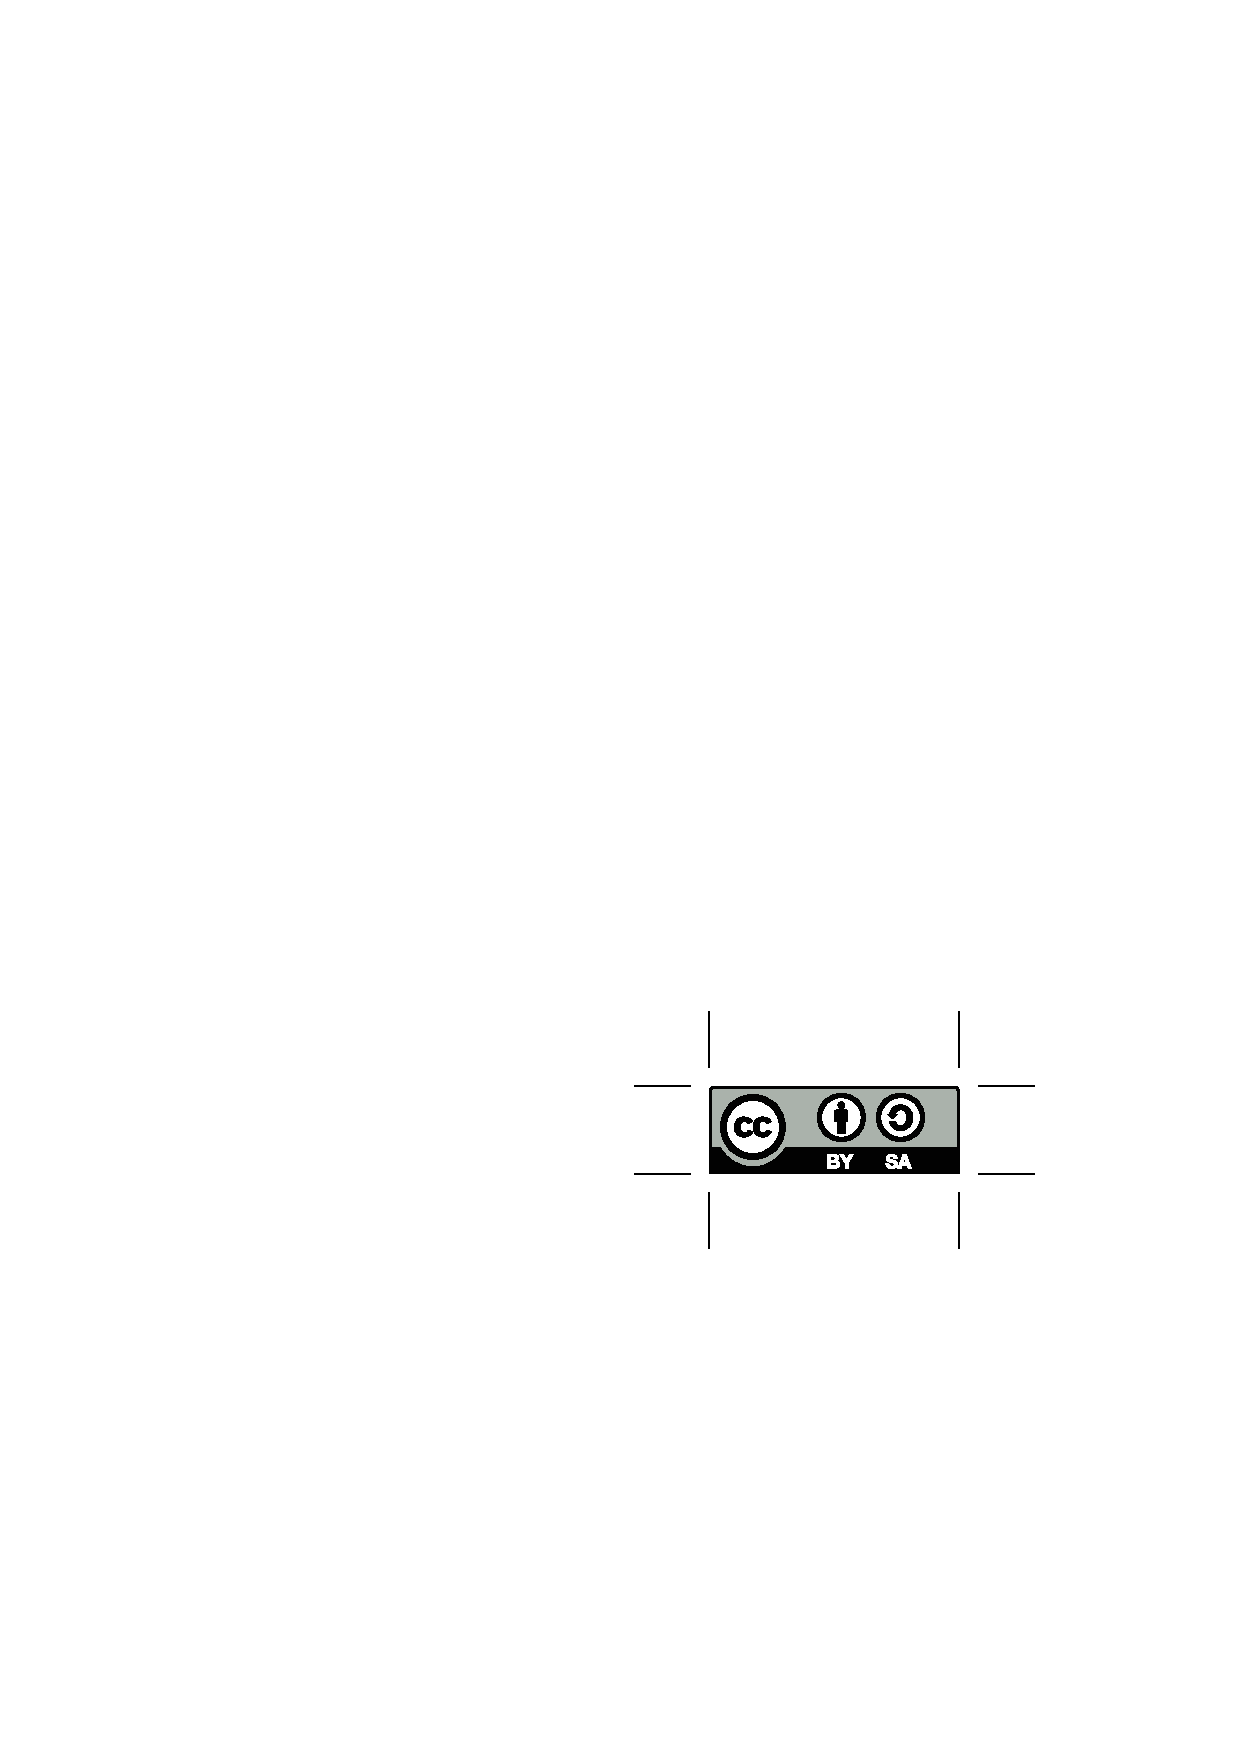
\includegraphics[width=.15\textwidth]{by-sa}
\doublespacing
% }}}

% Contents {{{
\cleardoublepage
\phantomsection
\addcontentsline{toc}{chapter}{\contentsname}
\tableofcontents
% %}}}

% List of figures {{{
\cleardoublepage
\phantomsection
\addcontentsline{toc}{chapter}{\listfigurename}
\listoffigures
%}}}

% List of tables {{{
\cleardoublepage
\phantomsection
\addcontentsline{toc}{chapter}{\listtablename}
\listoftables
% }}}

\chapter{Acknowledgements} %{{{

%}}}

\mainmatter

\chapter{Introduction} % {{{

\section{Certified systems at scale} %{{{
\label{ssec:certsys}

% preamble {{{

Certified software~\citep{shao10}
is software accompanied by
a mechanized, machine-checkable proof of correctness.
To construct a certified program,
we must not only write its code in a given programming language,
but also formally specify its intended behavior.
Then,
we must use specialized tools
to construct evidence that the program
indeed conforms to the specification.

%To achieve this,
%we need formal models of
%the languages in which
%the programs and other systems we wish to certify
%are described.
%The tools used to reason about them
%should be sound with respect to these models.
%Ideally,
%this will be demonstrated in an established,
%general-purpose proof assistant,
%diminishing the possibility that
%incorrect programs will be validated because of
%accidental or deliberate mistake
%in the software used to construct and check proofs.

The past decade has seen an explosion
in the scope and scale of practical software verification.
Researchers have been able to produce certified
compilers \citep{compcert},
program logics \citep{vst},
operating system kernels \citep{sel4,popl15},
file systems \citep{fscq},
processor designs \citep{safe,kami} and
more,
often introducing new techniques
and mathematical models.
In this context,
there has been increasing interest in
making these components
interoperable,
with the goal of
combining them---and their proofs of correctness---%
into larger certified systems.

%}}}

\subsection{The DeepSpec project} %{{{

For example, the DeepSpec project \citep{deepspec}
seeks to connect various components
specified and verified in the Coq proof assistant.
The key idea behind DeepSpec
is to use specifications as \emph{interfaces}
between components.
When a component providing a certain interface
has been verified,
client components can rely on this
for their own proofs of correctness.
Standardizing this process would make it possible
to construct large-scale certified systems
by assembling off-the-shelf certified components.

This approach promises benefits
beyond the potential increase in the scale of
certified systems.
As it stands,
a certified system is only
as trustworthy as its specification.
Indeed,
it is possible to prove a buggy system correct
with respect to a buggy specification.
If the specification is only validated by
a human expert subjecting it to careful examination,
these bugs could go unnoticed
and persist in the final system.
By contrast,
if the same specification is used as a premise
in the correctness proof of a client component,
its deficiencies will become apparent,
making it impossible to carry out this second proof.

Moreover,
internal specifications used
as intermediate steps
in the verification of a complex system
disappear from its external characterization
and no longer need to be trusted.
This reduces the ratio between the size of the system
and the size of the trusted specification.
%which must be trusted and understood
%to establish guarantees about the overall system.

%}}}

\subsection{CompCert} %{{{

To an extent,
these principles are already demonstrated in the structure of the
certified C compiler CompCert \citep{compcert}.
CompCert can emit assembly code
for PowerPC, ARM, RISC-V and x86 processors,
and supports an extensive subset of ISO C99
as its source language.
As a \emph{certified} compiler,
CompCert includes
language semantics for the source and target language,
and a proof of correctness relating the behaviors of
the source and target programs.

CompCert is often interfaced with source-level verification tools.
In that context,
the \kw{Clight} intermediate language
is often used as the source language.
\kw{Clight} is a simplified dialect of C
more amenable to formal reasoning.
The architecture-specific assembly language
targeted by CompCert is known as \kw{Asm}.

Like all components used in the DeepSpec project,
CompCert was specified and verified
in the Coq proof assistant.
The proof shows that if the compiler successfully transforms
a source program $p$ into a target program $p'$,
then the behavior of the target program
\emph{refines} that of the source program:
\[
  \begin{prooftree}
    \hypo{\kw{CompCert}(p) = p'}
    \infer1{\kw{Clight}[p] \supseteq \kw{Asm}[p']}
  \end{prooftree}
\]
In the statement above,
the semantics of the source and target programs
are expressed as the sets of traces
$\kw{Clight}[p]$ and $\kw{Asm}[p']$.
Each trace records a possible execution of the corresponding program
as a sequence of events.
The trace containment property
$\kw{Clight}[p] \supseteq \kw{Asm}[p']$
expresses that any possible behavior of
the target program~$p'$
is a possible behavior of the source program~$p$.

The key to this achievement
was the decomposition of CompCert
into compilation passes,
which were then verified individually.
When passes are composed to obtain the overall
C-to-assembly compiler
(Figure~\ref{fig:compcert}),
their correctness proofs can be composed as well
to establish the compiler's overall correctness theorem.
The final theorem does not mention the intermediate
programs or language semantics,
so that a user only needs to trust
the accuracy of the \kw{Clight} and \kw{Asm} semantics,
and the soundness of the proof assistant.

\begin{figure}
  \[
    \begin{prooftree}
      \hypo{p}
      \infer1[$\kw{Clight}$]{\module{\kw{SimplLocals}} }
      \infer1[$\kw{Clight}$]{\module{\kw{Cshmgen}} }
      \infer1[$\kw{Csharpminor}$]{\rule[-1em]{0pt}{3em}\vdots}
      \infer1[$\kw{Linear}$]{\module{\kw{Linarize}} }
      \infer1[$\kw{Mach}$]{\module{\kw{Asmgen}} }
      \infer1[$\kw{Asm}$]{p'}
    \end{prooftree}
    \qquad \Rightarrow \qquad
    \begin{prooftree}
      \hypo{p}
      \infer1[$\kw{Clight}$]{\module{\rule[-5em]{0pt}{11em}\kw{CompCert}} }
      \infer1[$\kw{Asm}$]{p'}
    \end{prooftree}
  \]
  \caption[Structure of the certified compiler CompCert]%
   {Structure of the certified compiler CompCert.
    The source program $p$ is progressively transformed
    into the target program $p'$ by successive compilation passes,
    depicted here as rectangular boxes.
    The horizontal line above each compilation pass
    depicts its source language,
    and the one below it depicts its target language.
    Two passes %and their semantic preservation properties
    can be composed when the target language of the first one
    corresponds to the source language of the second one.
    See also Table~\ref{tbl:passes}.}
  \label{fig:compcert}
\end{figure}

The introduction of CompCert in 2008
represented a breakthrough
in the scale and feasability of
certified software.
Since then,
CompCert itself
has been used as a platform other projects have built upon.
For example,
verification tools have been created with soundness proofs
connecting to CompCert \citep{vst,verasco}, and
the composition techniques used to verify CompCert
have been extended in various directions
\citep{compcompcert,sepcompcert,compcertm}.

%}}}

\subsection{CertiKOS} %{{{

The techniques used in CompCert
also provided a blueprint for the verification of
the operating system kernel CertiKOS
\citep{popl15,ccal,osdi16}
developed in the Yale FLINT group.
(I joined the FLINT group shortly before the effort
to verify a complete version of CertiKOS started.)

CertiKOS is divided into
several dozen \emph{certified abstraction layers},
which were specified and verified individually.
\emph{Layer interfaces} provide
an abstract view of a layer's functionality,
hiding the procedural details and low-level data representations
involved in its implementation.
A layer interface
enumerates the primitives implemented by a layer
and specifies their expected behavior.
Client code can then be verified in terms of
this abstract view
in order to build higher-level layers.

To make this possible,
we parametrized CompCert semantics
by a layer interface:
the expression $\kw{Asm}_L[C]$
denotes the set of traces generated by the client program $C$
running on top of the layer interface $L$.
Then a layer $M$
implements an \emph{overlay} interface $L_2$
on top of an \emph{underlay} interface $L_1$
when the following \emph{contextual refinement}
property holds:
\[
  \forall \, C \, \bdot \,
    \kw{Asm}_{L_2}[C] \supseteq \kw{Asm}_{L_1}[C + M] \,.
\]
Here,
the execution of the client code $C$ on top of the overlay $L_2$
serves as the specification.
The property shows that this specification
can be implemented
by running $C$ together with the layer implementation $M$
on top of the underlay interface $L_1$.

\begin{figure} % fig:certikos {{{
  \[
    \begin{prooftree}
      \hypo{C}
      \infer1[$\kw{TSyscall}$]{\module{M_n}}
      \infer1[$\kw{TTrap}$]{\module{M_{n-1}} }
      \infer1[$\kw{TTrapArg}$]{\rule[-1em]{0pt}{3em}\vdots}
      \infer1[$\kw{MATOp}$]{\module{M_2}}
      \infer1[$\kw{MATIntro}$]{\module{M_1}}
      \infer1[$\kw{PreInit}$]{C + M_n + \cdots + M_1}
    \end{prooftree}
    \qquad \Rightarrow \qquad
    \begin{prooftree}
      \hypo{C}
      \infer1[$\kw{TSyscall}$]{\module{\rule[-5em]{0pt}{11em}\kw{CertiKOS}} }
      \infer1[$\kw{PreInit}$]{C + \kw{CertiKOS}}
    \end{prooftree}
  \]
  \caption[Structure of the certified OS kernel CertiKOS]%
   {Structure of the certified OS kernel CertiKOS.
    Here, boxes represent certified abstraction layers
    and horizontal lines represent layer interfaces.
    The high-level client program $C$ is transformed
    into the complete low-level program $C + \kw{CertiKOS}$
    by linking it with the successive certified abstraction layers
    of CertiKOS.
    As before, the correctness properties of layers can be composed
    to derive a correctness property for the whole system.}
  \label{fig:certikos}
\end{figure}
%}}}

Certified abstraction layers
with compatible interfaces can then be chained together,
in the same way passes of a compiler
can be composed when the target language of one
corresponds to the source language of another.
This allows us to derive a contextual refinement property
for the whole kernel (Figure~\ref{fig:certikos}).
The system call interface of CertiKOS is specified
by the topmost layer interface $\kw{TSyscall}$,
and the basic facilities offered by the hardware
are formalized as the base layer interface $\kw{PreInit}$.
Then, by decomposing $\kw{CertiKOS} = M_n + \cdots + M_1$
into 37 certified abstraction layers,
we were able to derive the overall theorem:
\[
  \forall \, C \, \bdot \,
    \kw{Asm}_{\kw{TSyscall}}[C]
    \supseteq
    \kw{Asm}_{\kw{PreInit}}[C + \kw{CertiKOS}] \,.
\]

%}}}

\subsection{Horizontal composition} %{{{

In addition to
the \emph{vertical} composition principles outlined above,
CompCert and CertiKOS provide limited forms of
\emph{horizontal} composition,
which allow individual programs and layer implementations
to be decomposed futher.

In CompCert,
this is used to model \emph{separate compilation}.
The original correctness theorem of CompCert
only characterized the compilation of a whole program,
but in practice C programs usually consist of
several \texttt{.c} files, known as \emph{compilation units}.
These components are compiled independently,
and the results are combined through \emph{linking} to build
an executable image.
To reflect this,
\citet{sepcompcert}
introduced a notion of program linking ($+$), and
generalized the correctness theorem of CompCert
to the separate compilation property:
\[
  \begin{prooftree}
    \hypo{\forall \, 1 \le i \le k \, \bdot \,
      \kw{CompCert}(p_i) = p_i'}
    \infer1{\kw{Clight}[p_1 + \cdots + p_k] \supseteq
      \kw{Asm}[p_1' + \cdots + p_k']}
  \end{prooftree}
\]

Likewise,
in CertiKOS the verification of a given layer
can be decomposed into
the verification of the individual functions
which constitute its implementation.
This is achived through the \emph{layer calculus}
presented in Chapter~\ref{sec:cal}.

%}}}

\subsection{Challenges} %{{{

The vertical and horizontal composition principles
used in CompCert and CertiKOS
enabled the construction of certified systems
of significant size.
However, extending them to build large-scale certified systems
out of disparate certified components
is difficult.
A key aspect enabling composition in CompCert and CertiKOS
is the uniformity of the models underlying
their language semantics and correctness proofs.
By contrast,
across certified software projects
there exists a great diversity
of semantic models and verification techniques.
This makes it difficult to formulate
specifications for interfacing specific projects,
let alone devise a general method
for connecting certified components.

Worse yet,
this diversity is not simply a historical accident.
The semantic models
used in the context of individual verification projects
are often carefully chosen
to make the verification task tractable.
The semantic model used in CompCert alone
has changed multiple times,
addressing new requirements and techniques
which were introduced alongside
new compiler features and optimizations~\citep{compsem}.

Given the difficulty of verification,
it is essential
to preserve this flexibility in the choice of models
used to verify individual components.
To make it possible to link components
verified using a variety of paradigms,
we must then identify a model
expressive enough to embed
the semantics, specifications and correctness proofs
of all these paradigms.
The model should provide
high-level composition and reasoning principles,
allowing us to construct large-scale certified systems.

%}}}

%}}}

\section{General models for system behaviors} %{{{
\label{ssec:genmodel}

Fortunately,
there is a wealth of semantics research to draw from
as we attempt to design general models for certified components.
I outline some of it below.

\subsection{Symmetric monoidal categories} %{{{

As a whole,
category theory provides
a general taxonomy of
compositional structures found
across mathematics.
In a category,
two components (morphisms) can be chained together when
the interface which the first one provides
(its target object)
matches the interface which the second one relies on
(its source object).
For example,
as described above,
compilation passes and certified abstraction layers
both constitute categories.

Categories can be equipped with additional structure.
In particular,
\emph{symmetric monoidal categories}
allow components to be connected
not only in series~($\circ$)
but also in parallel~($\otimes$),
as illustrated by the following rules:
\[
  \begin{prooftree}
    \hypo{f : A \rightarrow B}
    \hypo{g : B \rightarrow C}
    \infer2{g \circ f : A \rightarrow C}
  \end{prooftree}
  \qquad
  \qquad
  \begin{prooftree}
    \hypo{f_1 : A_1 \rightarrow B_1}
    \hypo{f_2 : A_2 \rightarrow B_2}
    \infer2{f_1 \otimes f_2 : A_1 \otimes A_2 \rightarrow B_1 \otimes B_2}
  \end{prooftree}
\]
Many kinds of systems and processes
exhibit this structure \citep{rosetta}.
The basic setup can be refined by introducing additional constructions,
for instance modeling
feedback loops (traced monoidal categories) or allowing
wires to run in both directions
($*$-autonomous categories).

Symmetric monoidal categories appear in different forms
in many approaches to logic and programming language semantics.
For example,
\emph{cartesian closed} categories
correspond
to models of the simply typed lambda calculus,
and are a special case of symmetric monoidal categories.
However,
%in contrast with the stronger notion of
%cartesian closed category,
symmetric monoidal categories in general do not require
multiple components to be able to connect to the same interface
($\Delta : A \rightarrow A \otimes A$),
giving us more flexibility when modeling resources.
In the same way the simply-typed lambda calculus provides
an internal language for cartesian closed categories,
various fragments of \emph{linear logic} provide
internal languages for various kinds of symmetric monoidal categories.

In general,
the theory of symmetric monoidal categories
constitutes a repository of algebraic structures
formalizing the compositional aspects of
all kinds of systems,
and can guide the design
of general models.

%}}}

\subsection{Game semantics} %{{{

A specific way to construct symmetric monoidal categories
is \emph{game semantics} \citep{cspgs},
which uses two-player \emph{games} to describe
the possible interactions between
program components and their environment,
and uses \emph{strategies} for these games
to represent the externally observable behavior
of components.
%(\S\ref{sec:bg:gamesem}).

Game semantics is a synthesis
of various approaches to programming language semantics.
It is a form of \emph{denotational semantics},
defining the behavior of complex programs
in terms of the behavior of their components.
However,
since it models components
by describing their interactions across time,
game semantics also exhibits a strong \emph{operational} flavor.
Finally,
the usual construction of strategies used in game semantics
is a variation on the \emph{trace semantics}
used in the context of process algebras
and concurrent semantics.

An early success of game semantics
was the formulation of the first satisfactory
fully complete models for
the programming language PCF \citep{pcfajm,pcfho}.
Since then,
game semantics have provided fully complete models
for a wide variety of languages,
incorporating features such as
state \citep{gsia},
control \citep{gscontrol},
general references \citep{gsgr},
concurrency \citep{gsconcur}
and more.

There are deep connections between
game semantics and linear logic \citep{gsnecessary},
and hence symmetric monoidal categories,
hinting at its promise
as a general approach for modeling
various kinds of systems and processes.
In particular,
the typed aspect of many game models
makes them well-suited for
describing the behavior of heterogeneous systems.
However,
the generality of game models
often translates to a fair amount of complexity,
which imposes a high barrier to entry for practitioners
and makes them difficult to formalize in a proof assistant.

%}}}

\subsection{Algebraic effects} %{{{

While more restricted,
the framework of \emph{algebraic effects} \citep{effadq}
is sufficient for many modeling tasks,
fits within the well-known monadic approach
to effectful and interactive computations,
and can be seen as a particularly simple version
of game semantics.

In this framework,
computations are modeled as \emph{terms}
in an algebra whose operations correspond to
the available effects. %(\S\ref{sec:eff}).
The computation proceeds inward,
with each function symbol representing an occurence of an effect,
and each argument representing a possible way
for the computation to be continued
after the effect has occurred.

An advantage of this approach is that
the methods and results of universal algebra
become available to reason about effectful computations.
Equational theories can be used to characterize
the behavior of effects, and interpretations
of one effect algebra into another model
\emph{effect handlers} \citep{eff}.
The \emph{free monad} associated to an algebra
can be used to recover the more familiar
monadic model of computational effects \citep{monads}.
Along these lines,
\emph{interaction trees} \citep{itree}
have been developed
and formalized in the Coq proof assistant
for use in and across
several DeepSpec projects.

Alegbraic effects can also be understood as
a limited form of game semantics:
signatures can be interpreted as simple games,
and the abstract syntax trees of terms
can be interpreted as strategies.
However,
their restriction to first-order computation
make them easier to formalize and reason about
than more general notions of games.

%\section{General formulations for correctness proofs}
%\label{ssec:genform}

%}}}

\subsection{The refinement calculus} %{{{

%Finally,
While game semantics
and effect systems
have been proposed
for a wide variety of programming languages,
there has been comparatively less focus
on specifications and correctness properties
for game semantics and algebraic effects.
By contrast,
the general approach of \emph{stepwise refinement},
suggests a uniform treatment of programs and specifications.
It has been studied extensively in the context of
Dijkstra's predicate transformer semantics \citep{gc}, and
in the framework known as the \emph{refinement calculus} \citep{refcal}.

In refinement-based approaches,
programs and specifications are expressed in a common language,
and a certified program is constructed in an incremental manner,
by applying a series of correctness-preserving transformation
to the (abstract and declarative) specification
until we obtain a (concrete and executable) program.
Correctness preservation is expressed
by a reflexive and transitive \emph{refinement} relation.
Language constructions are monotonic with respect to this relation,
so that elementary refinement rules
can be applied congruently within any program context.

To make it possible to express specifications,
the language is extended with non-executable constructions.
In particular,
the refinement calculus includes infinitary versions of both
\emph{angelic} and \emph{demonic} nondeterministic choice operators.
In its modern presentation,
the refinement calculus is formulated in a lattice-theoretic framework
where joins ($\sqcup$) and meets ($\sqcap$)
correspond respectively to angelic and demonic choices.
The resulting language is remarkably expressive
and requires very few additional primitive constructions.
The duality inherent in this approach
also lends itself to game-theoretic interpretations,
and indeed the semantics of the refinement calculus
can be expressed as a two-player game between
the angel and the demon.

%Like all approaches in the lineage of Hoare logic
%and predicate transformer semantics,
%the refinement calculus is limited to
%modeling imperative programs.
%[However,
%M\&T propose to extend it to terms and functional programming
%by constructing the FCD blah blah.]
%
%[Also: describe the idea of the \emph{refinement calculus hierarchy}
%(general and difficult <-> specific and easy to reason about
%and string properties).
%More than one level of ``semantics''
%Notions of ``syntax'' and ``semantics'' are relative concepts.]

%}}}

%}}}

\section{Compiling certified components} %{{{

There are two ways to look at CompCert
in the context of software verification:
as a certified system
with an interesting structure,
or as a tool
we can use to build certified programs.

\subsection{CompCert as a certified system}

Until now,
I have mostly discussed
CompCert as an example of certified system,
describing the compositional structures used in
its construction as a precedent for the development of
certified systems of significant size.

From this point of view,
the language semantics
formalized alongside the compiler's code
are components of its specification,
used to express the behavior expected of
a C compiler
and to formulate the compiler's correctness theorem.
The long-standing effort to refine and generalize
these semantics and proofs
can be understood as
an attempt to model real-world compiler usage
more accurately,
preventing bugs in the compiler
from making it through the verification process
due to simplifications in its specification.

Connecting CompCert with other components
could mean combining the correctness proof of CompCert
with that of a certified assembler
and certified linker,
perhaps even with a certified processor design.
By verifying a larger portion of the toolchain end-to-end,
this would provide a stronger guarantee
that the source programs written by the user
will ultimately be executed in a way that conforms to
the C standard.
Work in this direction includes \cite{stackaware}.

\subsection{CompCert as a tool for building certified systems}

CompCert is also used as a tool
for constructing other certified systems.
For example,
CertiKOS uses the assembly semantics formalized in CompCert
to model the execution of the kernel's code
and to express the correctness property
which it must satisfy.
In addition,
CompCert is used to compile the portions of the kernel
which are written in C,
and the compiler's correctness theorem
allows us to use code proofs carried out
with respect to the source code
to prove the compiled assembly code correct.

CompCert serves in this case as
a rudimentary \emph{framework} for the construction of
certified C and assembly programs
in the Coq proof assisant.
From this point of view,
efforts to increase the precision and flexibility
of the compiler's correctness theorem
have made this framework more general and compositional.

\subsection{Intergrating CompCert into a general-purpose model}

Given the specialized nature
of CompCert's semantics and proofs,
it is difficult to imagine
that ``CompCert as a framework'' itself
could be extended
to allow the construction of general certified systems
spanning a wide range of abstraction levels.
Still,
given the importance of compilers in
the construction of present-day computer systems,
and the importance of CompCert in the formal methods landscape,
its integration into any framework
attempting to tackle end-to-end verification
should be a litmus test,
and would provide immediate benefits:
\begin{itemize}
  \item
    CompCert uses transition systems to define language semantics.
    Embedding these transition systems
    into a general model
    would immediately augment that model with
    a semantics for C and assembly programs.
    If we use a version of CompCert transition systems
    which can express the behavior of individual translation units,
    this would also give us the ability to
    formally interface, at a granular level,
    program components with components of different kinds,
    for example
    file systems, network services, or hardware devices.
  \item
    Then,
    in conjunction with a sufficiently precise
    correctness theorem,
    CompCert would not simply provide
    a certified compiler,
    but in fact
    a \emph{compiler of certified program components}.
    Correctness proofs characterizing
    the interactions of a component's source code with the environment
    could be transferred in a systematic way
    to the compiled code.
\end{itemize}

Unfortunately,
despite the abundance of research
extending CompCert in this direction,
no current extension is flexible enough to be used in this way
(\S\ref{sec:compcertlim}).
As noted by \citet{next700},
the problem of certified compositional compilation
is extremely complex and challenging,
lacking even a commonly accepted definition.
In fact,
as illustrated by the connections between
certified abstraction layers and
certified compilation,
the very extensive form of
compositional certified compilation
which I describe above
is almost as challenging to address
as the broader problem of
modeling heterogenous certified components.

On the other hand,
this means that the techniques and conceptual framework
developed in this thesis
are well-suited
for understanding and tackling this problem,
and indeed the culmination of my work
is a version of CompCert
which solves this challenge.

%}}}

\section{Contributions} %{{{
\label{ssec:contrib}

The central claim of this dissertation is that a synthesis
of %the existing research on
game semantics, algebraic effects, and the refinement calculus
can be used to construct a hierarchy of semantic models
suitable for constructing large-scale, heterogeneous certified systems:
\begin{itemize}
  \item
    Part~\ref{part:prelim} introduces relevant background
    and the general approach of
    \emph{refinement-based game semantics}.
    A reexamination of the fundamentals of game semantics
    under the lens of dual nondeterminism
    invites us to regard plays as \emph{elementary specifications}
    for the behaviors of interactive systems.
    The completion of plays
    with arbitrary angelic and demonic choices
    yields a notion of \emph{strategy specification},
    which provides support for
    stepwise refinement and data abstraction
    in the context of game semantics.
  \item
    Part~\ref{part:rbgs} demonstrates the use of this approach
    in the context of certified abstraction layers.
    Starting from the layer calculus of CertiKOS,
    I construct increasingly expressive models
    where layer interfaces, layer implementations and
    simulation relations
    can be treated in a uniform and compositional way.
  \item
    Part~\ref{part:compcerto}
    presents my work on the certified compiler CompCert.
    I examine existing models and techniques
    under the lens of refinement-based game semantics,
    and articulate why none of the existing
    CompCert extensions can be integrated within
    the framework in a completely satisfactory way.
    I then introduce CompCertO,
    the first extension of CompCert suitable
    for this use,
    which nevertheless avoids much of the complexity
    found in previous approaches.
\end{itemize}

Most of this work has been formalized in the Coq proof assistant.
As I am writing this,
the beginning of a Coq library
for refinement-based game semantics
is available at:
\begin{center}
  \url{https://github.com/CertiKOS/rbgs/}
\end{center}
A complete implementation of CompCertO
can also be found at the following address:
\begin{center}
  \url{https://github.com/CertiKOS/compcert/tree/compcerto}
\end{center}

%}}}

%They could be embedded in turn
%into more general game models, for instance where concurrency
%could be expressed in a more natural way.

%}}}

\part{Preliminaries} \label{part:prelim}

\chapter{Background} % {{{

Refinement-based game semantics combines
several lines of research.
This chapter aims to provide a short introduction to each one,
and give the reader a sense of how they relate to one another.

I begin
by outlining in \S\ref{sec:principles} general principles
which can be used in the construction of certified systems.
In the following sections,
I present
the \emph{refinement calculus} (\S\ref{sec:refcal}),
\emph{logical relations} (\S\ref{sec:lr}),
\emph{game semantics} (\S\ref{sec:bg:gamesem}),
\emph{algebraic effects} (\S\ref{sec:eff}) and
\emph{monads} (\S\ref{sec:eff:mon}).

\section{Building certified systems} \label{sec:principles} %{{{

\subsection{Semantic domains} %{{{

The goal of certified system design is
to create a formal description of
the system to be constructed (the program),
while ensuring
through careful analysis
that the system
will behave properly.
To this end,
we assign
to every system $p \in P$
a mathematical object $\llbracket p \rrbracket \in \mathbb{D}$
representing its behavior.
I will call the set $\mathbb{D}$ a \emph{semantic domain}.

\begin{example}[Trace semantics] \label{ex:trsem} %{{{
In CompCert,
the behaviors of programs are ultimately expressed
as sets of traces.
Each trace records a possible execution of the program,
as a finite or infinite sequence of externally observable events
taken from a set $\mathbb{E}$.
The program may then
terminate with an exit status $r \in \kw{int}$,
exhibit an undefined behavior ($\lightning$)
or silently diverge ($\Uparrow$).
The corresponding semantic domain can be defined as:
\[
  \mathbb{D}_\kw{CompCert} :=
    \mathcal{P}
      (\mathbb{E}^*\kw{int} +
       \mathbb{E}^*{\lightning} +
       \mathbb{E}^*{\Uparrow} +
       \mathbb{E}^\omega)
  \,.
\]
\end{example}
%}}}

In the remainder of this section I elucidate
the structure and properties of $\mathbb{D}$
necessary to the process of building
large-scale certified systems.

%}}}

\subsection{Specifications and refinement} %{{{

System design starts with a set of requirements
on the behavior of the system to be constructed
(the specification).
These requirements do not capture every detail
of the eventual system,
but delineate a range of acceptable behaviors.

In refinement-based approaches,
programs and specifications are interpreted in the same
semantic domain $\mathbb{D}$,
which is equipped with a \emph{refinement} preorder
${\refby} \subseteq \mathbb{D} \times \mathbb{D}$.
The proposition $\sigma_1 \refby \sigma_2$
asserts that $\sigma_1$ is refined by $\sigma_2$.
The correctness of a system description $p \in P$
with respect to a specification $\sigma \in \mathbb{D}$
can then be formulated as
$\sigma \refby \llbracket p \rrbracket$.

Refinement is intended to be a correctness-preserving relation.
For a set
$\mathbb{P} \subseteq \mathcal{P}(\mathbb{D})$
of properties of interest
and for two semantic objects $\sigma_1, \sigma_2 \in \mathbb{D}$,
the following property holds:
\[
  \sigma_1 \refby \sigma_2 \:\Rightarrow\:
  \forall P \in \mathbb{P} \bdot
    P(\sigma_1) \Rightarrow P(\sigma_2) \,.
\]
Note that in particular,
the property $P_\sigma(x) \: := \: \sigma \refby x$
is always preserved in this way.

\begin{example}[Trace containment]
In the trace semantics of CompCert,
the set of traces associated with the source program
is understood as a set of \emph{permissible} behaviors
for the target program.
As a first approximation,
the corresponding notion of refinement is
\emph{trace containment},
expressed by the superset relation $\supseteq$,
so that for example
$\kw{Clight}[p] \in \mathbb{D}_\kw{CompCert}$
is refined by
$\kw{Asm}[p'] \in \mathbb{D}_\kw{CompCert}$
when
$
  \kw{Clight}[p] \supseteq \kw{Asm}[p']
$.
Any property $P(\sigma)$
asserting that \emph{all} traces
$t \in \sigma \in \mathbb{D}_\kw{CompCert}$
satisfy a given condition
will be preserved by trace containment.

In fact,
CompCert also allows undefined behaviors
to be refined by more specific ones,
which makes the refinement relation
slightly more sophisticated.
See Chapter~\ref{sec:compcert-sem} for details.
\end{example}

%}}}

\subsection{Compositionality} %{{{

Complex systems are built by assembling components
whose behavior is understood,
such that their interaction achieves a desired effect.
The syntactic constructions of
the language used to describe systems
correspond to the ways in which they can be composed.

To enable compositional reasoning,
a suitable model must provide an account of
the behavior of a system
in terms of the behavior of its parts.
For instance,
if the language contains a binary operator
${+} : P \times P \rightarrow P$,
then the semantic domain should be equipped with
a corresponding operation
${\oplus} : \mathbb{D} \times \mathbb{D} \rightarrow \mathbb{D}$.
Ideally,
the operation $\oplus$
will characterize $+$ exactly:
\begin{equation}
  \llbracket p_1 \rrbracket \oplus \llbracket p_2 \rrbracket
  =
  \llbracket p_1 + p_2 \rrbracket
  \,.
  \label{eqn:compositionality}
\end{equation}

\begin{example}
Denotational semantics are compositional by nature.
The behavior of program components
is defined recursively on their structure,
so that (\ref{eqn:compositionality}) holds \emph{by definition}.
\end{example}

In the context of refinement-based verification,
we can regard $\oplus$ as a \emph{specification} for $+$,
and it is sufficient to establish that:
\begin{equation}
  \llbracket p_1 \rrbracket \oplus \llbracket p_2 \rrbracket
  \refby
  \llbracket p_1 + p_2 \rrbracket \,.
  \label{eqn:compositional-correctness}
\end{equation}

\begin{example}[Linking]
CompCert approximates \emph{linking}
as an operator $+$ which merges programs.
In CompCertO,
the semantic model is equipped with a
\emph{horizontal composition} operation $\oplus$,
which provides a specification for the linking operator.
In particular, the correctness of assembly linking
is established in Thm.~\ref{thm:asmlinking} as
$
  \kw{Asm}(p_1) \oplus \kw{Asm}(p_2) \refby
  \kw{Asm}(p_1 + p_2)
$.
\end{example}

%}}}

\subsection{Monotonicity} %{{{

Once a component has been shown to conform to a given specification,
we want to abstract it as a ``black box''
so that further reasoning can be done in terms of
the component's specification rather than its implementation details.
To support this,
we must establish that semantic composition operators
are compatible with refinement:
\[
  \begin{prooftree}
    \hypo{\sigma_1 \refby \sigma_1'}
    \hypo{\sigma_2 \refby \sigma_2'}
    \infer2{\sigma_1 \oplus \sigma_2 \refby \sigma_1' \oplus \sigma_2'}
  \end{prooftree}
\]
For example,
suppose we have two components $p_1$ and $p_2$,
where $p_2$ relies on $p_1$ for its operation,
and we want to verify that their combination $p_1 + p_2$
satisfies a specification $\sigma$.
Once we verify $p_1$ against its own specification
$\sigma_1 \refby \llbracket p_1 \rrbracket$,
by the monotonicity of ${\oplus}$ it is sufficient to show that
$\sigma \refby \sigma_1 \oplus \llbracket p_2 \rrbracket$:
\[
   \sigma \:\refby\:
   \sigma_1 \oplus \llbracket p_2 \rrbracket \:\refby\:
   \llbracket p_1 \rrbracket \oplus \llbracket p_2 \rrbracket \:\refby\:
   \llbracket p_1 + p_2 \rrbracket \,.
\]

%}}}

\subsection{Types} %{{{

In many cases,
systems are built out of components of various types
which can only be composed when their types are compatible.
Different semantic domains can then be used
to interpret components of different types.

As discussed in Chapter~\ref{chap:ct},
categories offer a systematic framework
to realize this separation.
Instead of a single set $\mathbb{D}$,
we use a category $\mathbf{D}$.
The objects $A \in \mathbf{D}$ correspond to
the possible types or interfaces alongside which
components can be connected.
A component which
uses an interface $A$ to
implement an interface $B$
can be modeled as a morphism
of type $A \rightarrow B$.
Categorical constructions can then be used
to formulate and characterize typed composition principles,
and the theory of \emph{enriched categories}
can be used to explore how these composition principles
interact with the structure of the semantic domains
$\mathbf{D}(A, B)$.

\begin{example}[Signatures] %{{{
The models introduced in this thesis use \emph{signatures},
discussed in \S\ref{sec:eff},
to enumerate the operations used and provided by program components.
Consequently,
the semantics of components are often expressed in categories
whose objects are signatures.
Morphisms of type $E \rightarrow F$
describe the behavior of components
which use the operations of the signature $E$
to implement the operations of the signature $F$.
Categorical products and other monoidal structures
can then be used to describe various
horizontal composition principles.
\end{example}
%}}}

%}}}

\subsection{Abstraction} %{{{

Large-scale systems operate across multiple levels of abstraction.
Each abstraction level brings its own understanding of the interaction
between a component and its environment.
To reason across abstraction layers we need to give
an explicit account of how these different views
of a component's behavior
correspond to one another.

This is studied extensively
in the context of abstract interpretation \citep{aif}.
Suppose $\mathbb{D}_1$ is the concrete domain
and $\mathbb{D}_2$ is the abstract one.
To establish a correspondence between them,
the most general approach is to define a \emph{soundness relation}
$\rho \subseteq \mathbb{D}_2 \times \mathbb{D}_1$.
We expect $\rho$
to be compatible with refinement:
\[
  \begin{prooftree}
    \hypo{\sigma_2' \refby_2 \sigma_2}
    \hypo{\sigma_2 \mathrel{\rho} \sigma_1}
    \hypo{\sigma_1 \refby_1 \sigma_1'}
    \infer3{\sigma_2' \mathrel{\rho} \sigma_1'}
  \end{prooftree}
\]
In other words,
if $\sigma_2$ is an abstraction which soundly approximates
a concrete semantic object $\sigma_1$,
we can make $\sigma_2$ less precise or $\sigma_1$ more precise
and preserve this relationship.

Often there will be a more elementary description
of the correspondence,
based on the construction of the semantic domains,
as illustrated by the following example.

\begin{example} % CAL {{{
In the model of \emph{certified abstraction layers}
presented in Chapter~\ref{sec:cal},
the semantic domain used to model a layer interface
is built from a set of abstract states $S$.
To compare a layer interface formulated in terms of
a more concrete set of states $S_1$ with
a layer interface formulated in terms of
a more abstract set of states $S_2$,
we will use a relation $R \subseteq S_2 \times S_1$.
This relation can then be extended to the level of layer interfaces
as a soundness relation
${\le_R} \subseteq \mathbb{D}[S_2] \times \mathbb{D}[S_1]$,
asserting that $R$ is a simulation relation between
a layer interface in $\mathbb{D}[S_2]$ and
a layer interface in $\mathbb{D}[S_1]$.
\end{example}
%}}}

In the case of categorical semantics
where $\mathbb{D}_1 = \mathbf{D}(A_1, B_1)$
and $\mathbb{D}_2 = \mathbf{D}(A_2, B_2)$
are homsets,
the constituents of the soundness relation
may themselves be organized as a category
with the same objects as $\mathbf{D}$.
This induces a double category structure,
where horizontal morphisms are the semantic objects,
vertical morphisms are abstraction relationships,
and 2-cells correspond to the soundness relation.

\begin{example}[Simulation conventions in CompCertO] %{{{
Interactions between C compilation units
are understood very differently
from interactions betwen assembly-language components.
At the level of C,
cross-module interactions are defined in terms of
function calls;
invoking a function means assigning values
to the function's parameters,
initializing a new stack frame,
and finally executing the function's body.
At the assembly level, cross-module
interactions simply consist in branching to an address
outside of the current module with
a certain register state.
The \emph{calling convention} used by a compiler
specifies the correspondence between the two.

In the model used in CompCertO,
\emph{language interfaces}
describe the form of cross-component interactions
for a class of languages.
They play the role of objects,
and semantic domains are assigned a type $A \rightarrow B$
where $A$ and $B$ are the language interfaces
respectively used by outgoing and incoming calls.
In addition,
a \emph{simulation convention}
$\mathbb{R}_A : A_1 \Leftrightarrow A_2$
is used to formulate the correspondence between
the high-level language interface $A_1$ and
the low-level language interface $A_2$.
A simulation property can then be depicted as the 2-cell:
\[
  \begin{tikzpicture}[scale=0.8]
    \node (A1) at (-1,  2) {$A_1$};
    \node (A2) at (-1,  0) {$A_2$};
    \node (B1) at ( 1,  2) {$B_1$};
    \node (B2) at ( 1,  0) {$B_2$};
    \draw (A1) edge[->] node[auto] {$L_1$} (B1);
    \draw (A2) edge[->] node[below] {$L_2$} (B2);
    \begin{scope}[double equal sign distance, {Implies[]}-{Implies[]}]
      \draw (A1) edge[double] node[auto,swap] {$\mathbb{R}_A$} (A2);
      \draw (B1) edge[double] node[auto] {$\mathbb{R}_B$} (B2);
    \end{scope}
  \end{tikzpicture}
\]
\end{example}
%}}}

When semantic domains are rich enough,
there may be a most precise
abstraction $\sigma_2 \in \mathbb{D}_1$
for each concrete semantic object
$\sigma_1 \in \mathbb{D}_1$,
defining an abstraction function
$\alpha : \mathbb{D}_1 \rightarrow \mathbb{D}_2$
such that:
\[
  \sigma_2' \mathrel{\rho} \sigma_1
  \: \Leftrightarrow \:
  \sigma_2' \refby_2 \alpha(\sigma_1)
\]
Conversely,
there may be a most general $\sigma_1$
corresponding to each $\sigma_2$,
defining
a concretization function
$\gamma : \mathbb{D}_2 \rightarrow \mathbb{D}_1$
such that:
\[
  \gamma(\sigma_2) \refby_1 \sigma_1'
  \: \Leftrightarrow \:
  \sigma_2 \mathrel{\rho} \sigma_1'
\]
When both an abstraction and concretization function exist,
they are related by the property:
\[
  \gamma(\sigma_2) \refby_1 \sigma_1
  \: \Leftrightarrow \:
  \sigma_2 \refby_2 \alpha(\sigma_1)
\]
This corresponds to
the original formulation of abstract interpretation \citep{absint}
in terms of Galois connections \citep{pgc}.

%}}}

\subsection{Embedding} \label{sec:bg:embed} %{{{

It is often useful to first interpret the semantics of a component
in a restricted domain,
then embed this domain into a more general one:
\[
    p \in P
    \: \xrightarrow{\llbracket - \rrbracket} \:
    \sigma \in \mathbb{D}
    \: \stackrel{|-|}{\longhookrightarrow} \:
    |\sigma| \in \mathbb{D}'
\]
The elements of the restricted domain $\mathbb{D}$
will often have stronger properties,
or be expressed in a way which makes certain
proof methods more tractable.
The more general domain $\mathbb{D}'$
can then provide more expressivity
and additional algebraic structures,
and may embed the behaviors of different kinds of components,
but may be less amenable to domain-specific reasoning.

In this situation,
we will want the embedding
$|-| : \mathbb{D} \hookrightarrow \mathbb{D}'$
to preserve any relevant structure present in both
$\mathbb{D}$ and $\mathbb{D}'$.
For example,
in the case of categorical semantics,
this embedding will be a (faithful) functor
of the appropriate kind.

\begin{example}[Transition systems and trace semantics in CompCert] %{{{
As mentioned in Example~\ref{ex:trsem},
CompCert semantics
ultimately characterize the behavior of programs
in terms of traces.
However,
they are first defined as labelled transition systems,
and the correctness properties of compilation passes
are first proved as simulations.
An embedding then assigns to each transition system $L$
the set of traces $|L|$ characterizing
its observable behavior,
and a soundness proof shows that
under certain conditions,
simulation properties $L_1 \le L_2$
imply trace containment $|L_1| \supseteq |L_2|$.
\end{example}
%}}}

\begin{example}[Certified abstraction layers] %{{{
The theory of certified abstraction layers
developped in Chapter~\ref{sec:cal}
describes deterministic layer interfaces
and implementations.
Abstraction is expressed using simulation relations.
Layer interfaces, layer implementations and simulation relations
are represented as three different kinds of objects.

In Chapter~\ref{sec:intspec},
I show how this theory of certified abstraction layers
can be embedded into a more general framework
which supports dual nondeterminism,
allowing layer interfaces, layer implementations and simulation relations
to be represented as morphisms in a uniform way,
at the cost of a more sophisticated notion of refinement.

Finally in Chapter~\ref{sec:gamesem},
I outline a framework where the layers' states
can be encapsulated and hidden from
the descriptions of the layers' behaviors,
and again provide an embedding of the previous theory
into this more general one.
Layer correctness can be expressed
without simulation relations,
but the cartesian products
of layers sharing states (\S\ref{sec:layerprod})
are no longer available.

Each of these embeddings preserves categorical composition,
refinement, and tensor products.
\end{example}
%}}}

%}}}

%}}}

\section{The refinement calculus} \label{sec:refcal} % {{{

% Preamble {{{

Correctness properties for imperative programs
are often stated as triples of the form $\htr{P}{C}{Q}$
asserting that
when the program $C$ is started in a state which
satisfies the predicate $P$ (the \emph{precondition}),
then the state in which $C$ terminates
will satisfy the predicate $Q$ (the \emph{postcondition}).
For example:
\[
    \htr{\text{$\kw{x}$ is odd}\,}{\kw{x := x * 2}}{\,\text{$\kw{x}$ is even}}
\]
In the \emph{axiomatic} approach
to programming language semantics~\citep{hoare69},
inference rules
corresponding to the different constructions of the language
determine which triples are valid,
and the meaning of a program is identified with
the set of properties $\htr{P}{-}{Q}$
which it satisfies.

%}}}

\subsection{Dual nondeterminism} %{{{

Axiomatic semantics
can accommodate nondeterminism in two different ways.

In the program $C_1 \sqcap C_2$,
a \emph{demon} will choose which of $C_1$ or $C_2$ is executed.
For example,
the program $\kw{x := 2 * x} \: \sqcap \: \kw{x := 0}$
may be executed arbitrarily as $\kw{x := 2 * x}$ or $\kw{x := 0}$,
with no guarantee as to which branch will be chosen.
The demon works against us,
so that if we want $C_1 \sqcap C_2$ to satisfy
a given correctness property,
we need to make sure we can deal with either choice:
\[
  \begin{prooftree}
    \hypo{\htr{P}{C_1}{Q}}
    \hypo{\htr{P}{C_2}{Q}}
    \infer2{\htr{P}{C_1 \sqcap C_2}{Q}}
  \end{prooftree}
\]

Conversely,
in the program $C_1 \sqcup C_2$,
an \emph{angel} will decide whether $C_1$ or $C_2$ is executed.
The statement $\kw{x := x * 2} \: \sqcup \: \kw{x := 0}$
is more difficult to interpret than its demonic counterpart,
but rougly speaking it magically behaves as
$\kw{x := x * 2}$ or $\kw{x := 0}$
depending on the needs of its user.
If possible,
the angel will make choices which validate
the correctness property.
Therefore:
\[
  \begin{prooftree}
    \hypo{\htr{P}{C_1}{Q}}
    \infer1{\htr{P}{C_1 \sqcup C_2}{Q}}
  \end{prooftree}
  \qquad
  \begin{prooftree}
    \hypo{\htr{P}{C_2}{Q}}
    \infer1{\htr{P}{C_1 \sqcup C_2}{Q}}
  \end{prooftree}
\]

More generally,
a triple $\htr{P}{C}{Q}$
can be interpreted as a \emph{game}
between the angel and the demon \citep[Chapter 14]{refcal}.
The angel resolves the $\sqcup$ choices,
whereas the demon resolves the $\sqcap$ choices.
The triple is valid if there is a strategy
for the angel
to validate the correctness property.

%}}}

\subsection{Distributivity} %{{{

Note that in this setup,
$\sqcap$ and $\sqcup$ distribute over each other.
More precisely, for all $P, C_1, C_2, C_3, Q$:
\begin{align*}
  \htr{P}{C_1 \sqcap (C_2 \sqcup C_3)}{Q} \: &\Leftrightarrow \:
    \htr{P}{(C_1 \sqcap C_2) \sqcup (C_1 \sqcap C_3)}{Q} \\
  \htr{P}{C_1 \sqcup (C_2 \sqcap C_3)}{Q} \: &\Leftrightarrow \:
    \htr{P}{(C_1 \sqcup C_2) \sqcap (C_1 \sqcup C_3)}{Q}
\end{align*}

Consider the first equivalence above.
For the angel to have a winning strategy for
the left-hand side triple,
they must be able to win both $\htr{P}{C_1}{Q}$
and either $\htr{P}{C_2}{Q}$ or $\htr{P}{C_3}{Q}$.
Although the right-hand side triple
reverses the order between the angel and the demon's choices,
the angel can preemptively choose the left or right
disjunct depending on whether they can win
$\htr{P}{C_2}{Q}$ or $\htr{P}{C_3}{Q}$.
Likewise, if the angel can win the right-hand side,
then they have a winning strategy for the left-hand side as well.
The second equivalence corresponds to a similar situation
where the angel and demon have been exchanged.

%}}}

\subsection{Program refinement} %{{{

Instead of proving program correctness in one go,
\emph{stepwise refinement} techniques use a more incremental approach
centered on the notion of program refinement.
A refinement $C_1 \sqsubseteq C_2$
means that any correctness property satisfied by $C_1$
will also be satisfied by $C_2$:
\[
    C_1 \sqsubseteq C_2 \: := \:
    \forall P Q \bdot
      \htr{P}{C_1}{Q} \Rightarrow
      \htr{P}{C_2}{Q}
\]
We say that $C_2$ refines $C_1$
or that $C_1$ is refined by $C_2$.

Typically,
under such approaches,
the language is extended with constructions
allowing the user to describe
abstract specifications as well as
concrete programs.
Then the goal is to establish
a sequence of refinements
$C_1 \sqsubseteq \cdots \sqsubseteq C_n$
to show that a program $C_n$
correctly implements a specification $C_1$.
The specification may be formulated in
abstract, declarative terms,
but the program should only use executable constructions.

If the language is sufficiently expressive,
then a correctness property $\htr{P}{-}{Q}$
can itself be encoded \citep{specstm} as
a specification statement $\langle{}P,Q{}\rangle$
such that:
\[
    \htr{P}{C}{Q} \: \Leftrightarrow \:
    \langle{}P,Q{}\rangle \sqsubseteq C \,.
\]
In the context of refinement,
the properties associated with demonic and angelic choice
become:
\[
  \begin{prooftree}
    \hypo{C \sqsubseteq C_1}
    \hypo{C \sqsubseteq C_2}
    \infer2{C \sqsubseteq C_1 \sqcap C_2}
  \end{prooftree}
  \qquad
  \begin{prooftree}
    \hypo{C \sqsubseteq C_1}
    \infer1{C \sqsubseteq C_1 \sqcup C_2}
  \end{prooftree}
  \qquad
  \begin{prooftree}
    \hypo{C \sqsubseteq C_2}
    \infer1{C \sqsubseteq C_1 \sqcup C_2}
  \end{prooftree}
\]
Given the duality between the demon and angel,
it is then natural to interpret demonic and angelic choices
respectively as meets and joins
of the refinement ordering.

\subsection{Nondeterministic choice in specifications}

Until this point,
we have discussed demonic ($\sqcap$) and angelic ($\sqcup$) choices
as implementation constructs
(appearing to the right of $\sqsubseteq$),
taking the point of view of a client
seeking to use the program to achieve a certain goal.
However,
in this work they are used primarily
as \emph{specification} constructs
(appearing to the left of $\sqsubseteq$),
and we are interested in what it means
for a system to implement them.
%
As a specification, $C_1 \sqcap C_2$
allows the system to refine either one of $C_1$ or $C_2$, while
$C_1 \sqcup C_2$ requires it to refine
\emph{both} of them:
\[
  \begin{prooftree}
    \hypo{C_1 \sqsubseteq C}
    \infer1{C_1 \sqcap C_2 \sqsubseteq C}
  \end{prooftree}
  \qquad
  \begin{prooftree}
    \hypo{C_2 \sqsubseteq C}
    \infer1{C_1 \sqcap C_2 \sqsubseteq C}
  \end{prooftree}
  \qquad
  \begin{prooftree}
    \hypo{C_1 \sqsubseteq C}
    \hypo{C_2 \sqsubseteq C}
    \infer2{C_1 \sqcup C_2 \sqsubseteq C}
  \end{prooftree}
\]
In other words,
demonic choices
give us more
implementation freedom,
whereas angelic choices make a specification
stronger and more difficult to implement.
%Intuitively,
%the \emph{user} of a specification
%will need to be ready to handle any demonic choice
%made in that specification.
%The specification's implementer
%will have more freedom because they \emph{are} the demon.
%Conversely,
%angelic choice requires the implementation
%to behave appropriately
%no matter which alternative the user decides to rely on.
%Therefore,
Therefore we can think of demonic choices as
choices of the \emph{system}, % we are considering,
and think of angelic choices as
choices of the \emph{environment}.

\begin{remark}
The work presented in this thesis
borrows from various lines of research;
one difficulty is that
the conventions and notations they use
are often different and sometimes inconsistent.

As the discussion above illustrates,
in the literature on Hoare logic,
the reader is often invited to identify with
a \emph{user} of the program (the environment)
trying to ascertain the program's properties,
and the terminology of ``angelic'' and ``demonic''
is used accordingly.
By contrast,
descriptions of game semantics are often narrated
from the point of view of the \emph{system},
and in that context the terminology
associated with dual nondeterminism
can be counter-intuitive at first.
\end{remark}

\begin{figure}
  \centering
  \begin{tabular}{c@{\hspace{4em}}c}
    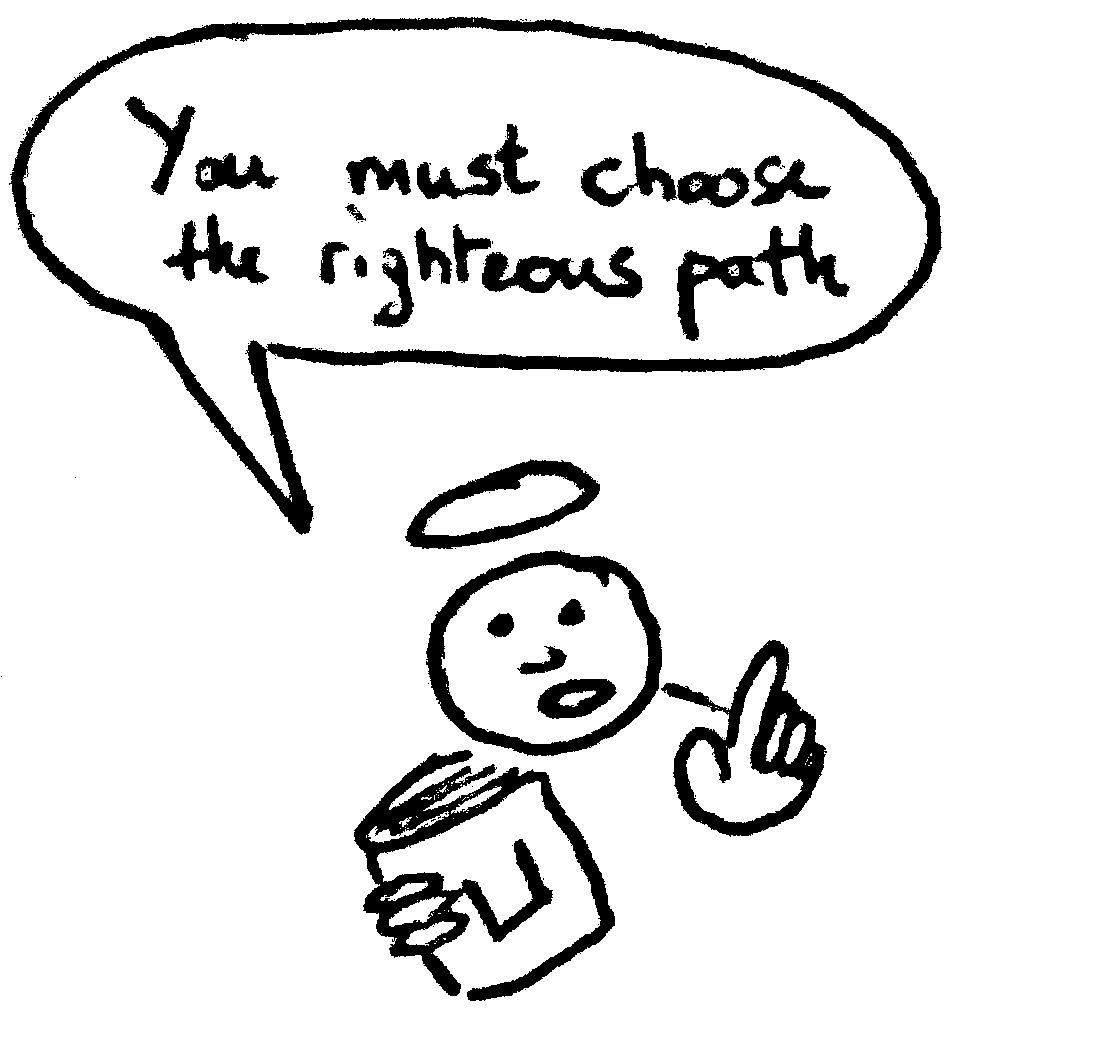
\includegraphics[scale=0.1]{angel} \hspace{1em} &
    \hspace{4em} \raisebox{0.66ex}{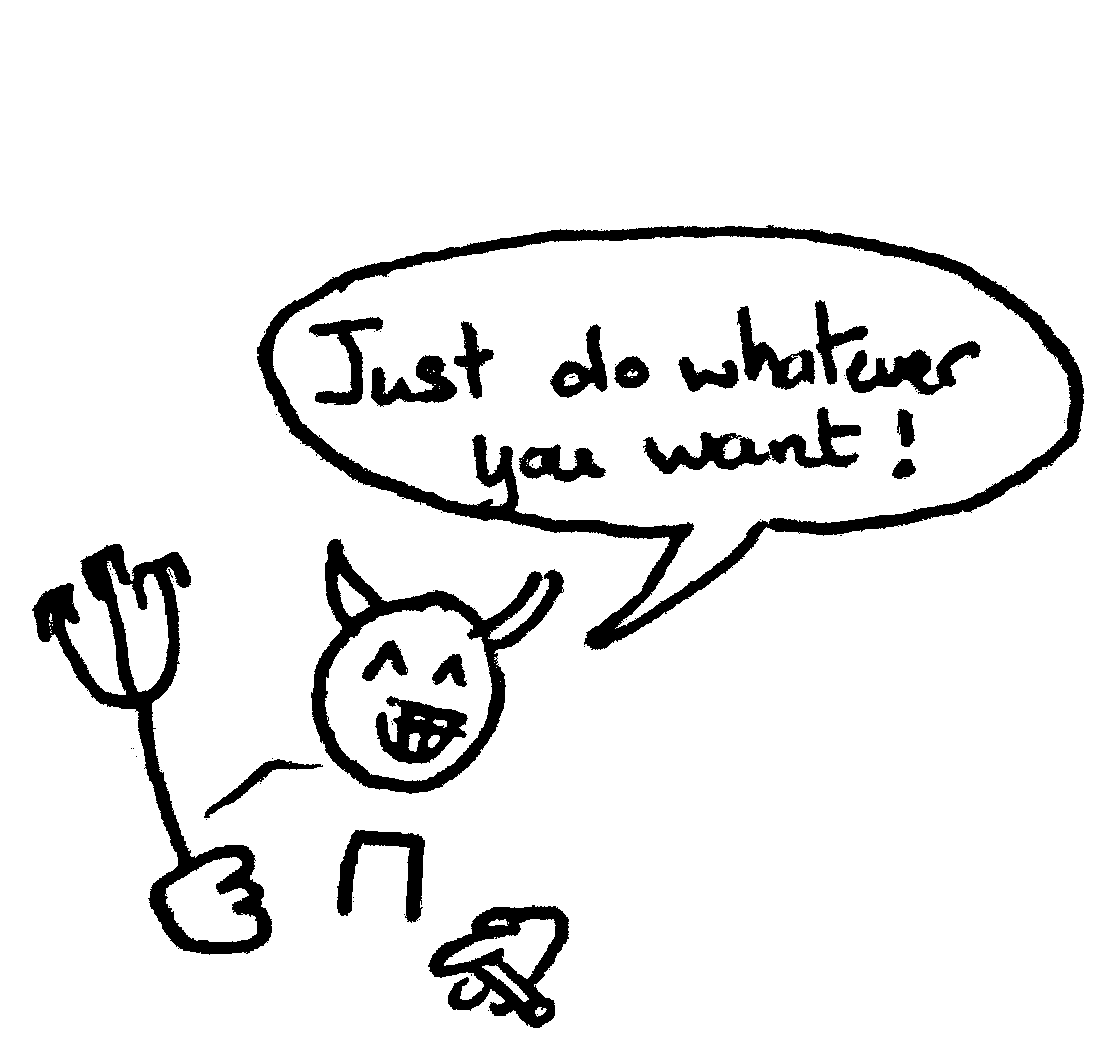
\includegraphics[scale=0.11]{demon}}
    \\
    (a) Angelic choice &
    (b) Demonic choice
  \end{tabular}
  \caption[Angelic and demonic choices in specifications]%
   {Angelic and demonic choices in specifications,
    from the perspective of the implementer.
    Life is hard when you're expected to behave like an angel!}
  \label{fig:angelspec}
\end{figure}

%}}}

\subsection{The refinement calculus} %{{{

The basic ingredients presented above have been studied systematically
in the \emph{refinement calculus},
dating back to Ralph-Johan Back's 1978 PhD thesis \citep{backthesis}.
In its modern incarnation,
the refinement calculus
subsumes programs and specifications with \emph{contracts}
featuring unbounded angelic and demonic choices \citep{refcal}.
These choice operators
constitute a \emph{completely distributive lattice}
with respect to the refinement ordering.

Dijkstra's \emph{predicate transformer} semantics \citep{gc}
is a natural fit for the refinement calculus,
but other approaches are possible.
For instance,
as mentioned above,
the understanding of contracts as a game between
the angel and the demon
can be formalized to provide a form of
game semantics for the refinement calculus.

In fact,
the refinement calculus can be presented as a \emph{hierarchy}
along the lines discussed in~\S\ref{sec:bg:embed},
whereby simpler models (state transformer functions, relations)
can be embedded into more general ones (predicate transformers)
in various structure-preserving ways.
This makes it possible to reason about simpler components
in a limited, stronger version of the framework,
while retaining the possibility of embedding them
in a setting
where more general constructions are available,
and where they can be composed with components
developed and analyzed in a different setting.
%This expressivity is highly desirable
%as a scalable approach to
%verifying heterogeneous systems.

However,
in its traditional formulation,
the refinement calculus only models imperative programs
with no side-effects beyond changes to the program state.
Recent research has attempted to extend the paradigm
to a broader setting,
and my work can be understood
as a step in this direction as well.

%}}}

%}}}

\section{Logical relations} \label{sec:lr} % {{{

Logical relations are structure-preserving relations
in the way homomorphisms are structure-preserving maps.
However,
logical relations are more compositional than homomorphisms,
because they do not suffer from the same problems
in the presence of mixed-variance constructions
like the function arrow %$\rightarrow$
\citep{lrp}.
In the context of typed languages,
this means that type-indexed logical relations
can be defined by recursion over the structure of types.

Logical relations have found widespread use in programming language theory.
For example,
unary logical relations can be used to establish
various properties of type systems:
a type-indexed predicate expressing a property of interest
is shown to be compatible with a language's reduction,
and to contain all of the well-typed terms of the language.
Binary logical relations can be used to capture
contextual equivalence between terms,
as well as notions such as non-interference or compiler correctness.
Relational models of type quantification yield
Reynold's well-known theory of relational parametricity,
and can be used to prove \emph{free theorems} that
all terms of a given generic type must satisfy.

For our purposes,
logical relations will provide a language to formulate
relationships between high-level and low-level behaviors,
or between specifications and implementations,
in a uniform and compositional way.


\subsection{Binary logical relations}

Logical relations can be of any arity,
but
I will focus on
binary logical relations.
Consider an algebraic structure $\mathcal{S}$.
A \emph{logical relation}
between two instances $S_1, S_2$ of $\mathcal{S}$
is a relation $R$
between their carrier sets,
such that the corresponding operations of $S_1$ and $S_2$
take related arguments to related results.
We write $R \in \mathcal{R}(S_1, S_2)$.

\begin{example}%[Logical relation of monoids] %{{{
\label{ex:monoid}
A monoid is a set with
an associative operation $\cdot$ and
an identity element $\epsilon$.
A~\emph{logical relation of monoids} between
$\langle A, \cdot_A, \epsilon_A \rangle$ and
$\langle B, \cdot_B, \epsilon_B \rangle$
is a relation $R \subseteq A \times B$
such that:
\begin{equation}
\label{eqn:monoidrel}
(u \mathrel{R} u' \wedge v \mathrel{R} v' \: \Rightarrow \:
 u \cdot_A v \: \mathrel{R} \: u' \cdot_B v')
\: \wedge \:
\epsilon_A \mathrel{R} \epsilon_B \,.
\end{equation}
\end{example}
%}}}

Logical relations used to reason about contextual equivalence
are often partial equivalence relations (PER).
By contrast, in the context of refinement,
most of the relations we use will not be symmetric.

\subsection{Relators} \label{sec:relators} %{{{

Logical relations between multisorted structures
consist of one relation for each sort,
between the corresponding carrier sets.
In the case of structures which include type operators,
we can associate to each base type $A$
a relation over its carrier set $\llbracket A \rrbracket$,
and to each type operator $T(A_1, \ldots, A_n)$
a corresponding \emph{relator}:
given relations $R_1, \ldots, R_n$ over
the carrier sets $\llbracket A_1 \rrbracket, \ldots, \llbracket A_n \rrbracket$,
the relator for $T$
will construct a relation $T(R_1, \ldots, R_n)$
over $\llbracket T(A_1, \ldots, A_n) \rrbracket$.
Relators for some common constructions are shown in Figure~\ref{fig:relators}.
Using them, the proposition (\ref{eqn:monoidrel}) can be reformulated as:
\[
  \cdot_A \ifr{R \times R \rightarrow R} \cdot_B
  \: \wedge \:
  \epsilon_A \mathrel{R} \epsilon_B \,.
\]

\begin{example} \label{ex:simrel} %{{{
Simulation relations are
logical relations of transition systems.
Consider the transition systems
$\alpha : A \rightarrow \mathcal{P}(A)$ and
$\beta : B \rightarrow \mathcal{P}(B)$.
A simulation relation $R \in \mathcal{R}(A, B)$
satisfies:
\[
  \begin{tikzcd}[scale=0.8]
    s_1 \arrow[r, "\alpha"]
        \arrow[d, dash, "R"'] &
    s_1' \arrow[d, dashed, dash, "R"] \\
    s_2 \arrow[r, dashed, "\beta"] &
    s_2'
  \end{tikzcd}
  \qquad
  \label{eqn:simrel}
  \begin{array}{r@{\,.\,}l}
    \forall s_1 \, s_2 \, s_1' &
      \alpha(s_1) \ni s_1' \wedge s_1 \mathrel{R} s_2 \Rightarrow
    \\[0.25ex]
    \exists s_2' &
      \beta(s_2) \ni s_2' \wedge s_1' \mathrel{R} s_2'
  \end{array}
\]
Using the relators in Figure~\ref{fig:relators},
we can express the same property
concisely and compositionally as:
\[
  \alpha \ifr{R \rightarrow \mathcal{P}^\le(R)} \beta \,.
\]
\end{example}
%}}}

\begin{figure} % fig:relators {{{
  \figsize
  \begin{align*}
    x \ifr{R_1 \times R_2} y \ \Leftrightarrow\  &
      \pi_1(x) \ifr{R_1} \pi_1(y) \wedge
      \pi_2(x) \ifr{R_2} \pi_2(y) \\
    x \ifr{R_1 + R_2} y \ \Leftrightarrow\  &
      (\exists \, x_1 \, y_1 \,.\,
        x_1 \ifr{R_1} y_1 \wedge
        x = i_1(x_1) \wedge
        y = i_1(y_1)) \\ \vee\ &
      (\exists \, x_2 \, y_2 \,.\,
        x_2 \ifr{R_2} y_2 \wedge
        x = i_2(x_2) \wedge
        y = i_2(y_2)) \\
    f \ifr{R_1 \rightarrow R_2} g \ \Leftrightarrow\  &
      \forall \, x \, y \,.\,
        x \ifr{R_1} y \Rightarrow
        f(x) \ifr{R_2} g(y) \\
    A \ifr{\mathcal{P}^\le(R)} B \ \Leftrightarrow\  &
      \forall \, x \in A \,.\,
      \exists \, y \in B \,.\,
      x \ifr{R} y \\
    A \ifr{\mathcal{P}^\ge(R)} B \ \Leftrightarrow\  &
      \forall \, y \in B \,.\,
      \exists \, x \in A \,.\,
      x \ifr{R} y
  \end{align*}
  \caption[A selection of relators]%
   {A selection of relators.
    The relators $\times$, $+$, $\rightarrow$ are standard.
    $\mathcal{P}^\le$ and $\mathcal{P}^\ge$ are asymmetric
    relators for the powerset type operator $\mathcal{P}$,
    which can be used to formulate simulations.
    }
  \label{fig:relators}
\end{figure}
%}}}

%}}}

\subsection{Kripke relations} \label{sec:klr} %{{{

Relations for stateful languages
often depend on the current state.
To address this,
Kripke logical relations
are parametrized over a set of state-dependent \emph{worlds}.
Components related at the same world
are guaranteed to be related in compatible ways.
We use the following notations.

\begin{definition} \label{def:klr} %{{{
A \emph{Kripke} relation is
a family of relations $(R_w)_{w \in W}$.
We write $R \in \mathcal{R}_W(A, B)$
for a Kripke relation between the sets $A$ and $B$.
For $w \in W$ I will write:
\[
\begin{array}{c@{\qquad}c}
    [w \Vdash R] \: := \: R_w &
    [\Vdash R] \: := \: \bigcap_{w} R_w
\end{array}
\]
\end{definition}
%}}}

A simple relation $R \in \mathcal{R}(A, B)$
can be promoted to a Kripke relation
$\lceil R \rceil \in \mathcal{R}_W(A, B)$
by defining $[w \Vdash \lceil R \rceil] := R$ for all $w \in W$.
More generally, for an $n$-ary relator $F$ we have:
\[
  \begin{prooftree}
  \hypo{
    F :
      \mathcal{R}(A_1, B_1) \,\times\,\cdots\,\times\,\mathcal{R}(A_n, B_n)
      \rightarrow \mathcal{R}(A, B)}
  \infer1{
    \lceil F \rceil :
      \mathcal{R}_W(A_1, B_1) \times \cdots \times \mathcal{R}_W(A_n, B_n)
      \rightarrow \mathcal{R}_W(A, B)}
  \end{prooftree}
\]
where for the Kripke relations $R_i \in \mathcal{R}_W(A_i, B_i)$:
\[
  [w \Vdash \lceil F \rceil (R_1, \ldots, R_n)] \: := \:
    F(w \Vdash R_1, \ldots, w \Vdash R_n)
\]
In the following,
I will use $\lceil - \rceil$ implicitly
when a relator appears in a context where
a Kripke logical relation is expected.
Since reasoning with logical relations
often involves self-relatedness,
I~will use the notation
$x :: R$ to denote $x \mathrel{R} x$.
For legibility, I also write
$w \Vdash x \mathrel{R} y$ for $x \ifr{w \Vdash R} y$
and $\Vdash x \mathrel{R} y$ for $x \ifr{\Vdash R} y$.

%}}}

\subsection{Modal relators} \label{sec:modrel} %{{{

Kripke logical relations are connected to
the Kripke semantics of modal logics.
In that context,
the set of world is used to index a model,
and the satisfaction of formulas may depend on
which world is considered.
The modality $\Diamond$ is then interpreted in terms of
an \emph{accessibility} relation, which I will write as $\leadsto$.
The formula $\Diamond P$ is satisfied in a world $w$
if there exists $w \leadsto w'$ such that $P$ is satisfied in $w'$.
Dually,
the formula $\Box P \equiv \neg (\Diamond \neg P)$
is satisfied in a world $w$
if $P$ is satisfied in \emph{all} worlds $w'$
accessible from $w$.

The accessibility relation essentially defines
a directed graph on the set of worlds,
and formulas constructed with $\Diamond$ and $\Box$
can explore the neighborhood of a given node.
A wide variety of complex data structures
can be seen as graphs;
modal logics and Kripke semantics
can be used to reason about such structures,
with countless applications in formal verification
\citep{modlog}.

Translating this approach to the setting of logical relations,
the modalities become relators.

\begin{definition} %{{{
A \emph{Kripke frame} is a tuple
$\langle W, {\leadsto} \rangle$, where
$W$ is a set of \emph{possible worlds} and
$\leadsto$ is a
binary \emph{accessibility relation} over $W$.
Then the Kripke relator $\Diamond$ is defined by:
\[
  w \Vdash x \ifr{\Diamond R} y \: \Leftrightarrow \:
    \exists \, w' \,.\, w \leadsto w' \wedge
      w' \Vdash x \mathrel{R} y
\]
\end{definition}
%}}}

%}}}

%}}}

\section{Game semantics} \label{sec:bg:gamesem} %{{{

% preamble {{{

Game semantics~\citep{gsll,gamesem99}
is a form of denotational semantics which
incorporates some operational aspects.
An early success of this approach was
the formulation of the first fully abstract models
of the programming language PCF \citep{pcfajm,pcfho}.
Typically,
game semantics interpret
types as two-player games
and terms as strategies for these games.
Games describe the form of the interaction
between a program component %of the corresponding type
(the \emph{system})
and its execution context
(the \emph{environment}).
Strategies
specify which move the system plays
for all relevant positions in the game.

Positions are usually identified with sequences of moves,
and strategies with the set of positions
a component can reach.
% depending on the possible behaviors of the environment
This representation makes
game semantics similar to
trace semantics of process algebras,
but it is distinguished
by a strong polarization between
actions of the system and the environment,
and between outputs and inputs.
This confers an inherent ``rely-guarantee'' flavor
to games which facilitates compositional reasoning
\citep{cspgs}.

For example,
in a simple game semantics resembling that of
Idealized Algol \citep{gsia},
sequences of moves corresponding to
the execution of $\kw{x := 2 * x}$
have the form:
\[
    \kw{run}\ph{run} \cdot
    \ul{\kw{read}_\kw{x}}\ph{rd} \cdot \pt{rd}n \cdot
    \ul{\kw{write}_\kw{x}[2n]}\ph{wr} \cdot \pt{wr}\kw{ok} \cdot
    \pt{run}\ul{\kw{done}} \quad (n \in \mathbb{N})
\]
The moves of the system have been underlined.
The environment initiates the execution with
the move $\kw{run}$.
The system move $\ul{\kw{read}_\kw{x}}$ then requests
the value of the variable $\kw{x}$,
communicated in response by the environment move $n$.
The system move $\ul{\kw{write}_\kw{x}[2n]}$ requests
storing the value $2n$ into the variable~$\kw{x}$,
and is acknowledged by the environment move $\kw{ok}$.
Finally, the system move $\ul{\kw{done}}$
expresses termination.
The gray arrows show the relationships
between questions and their corresponding answers,
but in the simple game models that I will consider
they are not part of the formalism.

%}}}

\subsection{Games} \label{sec:mainideas:gs:games} %{{{

A game is defined by a set of moves
players will choose from,
as well as a stipulation of which
sequences of moves are valid.
We focus on two-player, alternating games
where the environment plays first and
where the players
each contribute every other move.
As above, when typesetting examples,
we underline the moves of the system.

\begin{example}
In the game of chess,
moves are taken in the set $\{a1 \ldots h8\} \times \{a1 \ldots h8\}$.
From the perspective of the player
with black pieces,
a valid sequence of moves may look like:
\[ e2e4 \cdot \ul{c7c5} \cdot c2c3 \cdot \ul{d7d5} \cdots \]
\end{example}

%The games we use to model low-level components
%will rely on the following constructions.

Most game semantics
include additional structure
in the description of games.
The set of moves is usually partitioned
into system and environment moves ($M = M^\kw{O} \uplus M^\kw{P}$),
and into questions and answers ($M = M^\que \uplus M^\ans$).
Game models for high-order languages are often more complex,
and include \emph{justification pointers}
encoding the causal structure of the interaction.

%While the game $\mathcal{C}$
%is extremely simple,
The compositionality of game semantics
comes from the ways in which complex games can be derived from simple ones,
and used to interpret compound types.
For example,
in the game $A \times B$
the environment initially chooses whether to play
an instance of $A$ or an instance of $B$.
The game $A \rightarrow B$ usually consists of
an instance of $B$ played
together with instances of $A$
started at the discretion of the system,
where the roles of the players are reversed.
%and which correspond to
%the multiple accesses to the argument values
%allowed by most $\lambda$-calculi.

%}}}

\subsection{Strategies} \label{sec:bg:strat} %{{{

The \emph{plays} of a game are sequences of moves;
they both identify a position in the game
and describe the succession of actions that led to it.
Most game models of sequential computation
use \emph{alternating} plays,
in which
the system and environment each contribute
every other move.
It is also common to require the environment to play first
and to restrict plays to even lengths,
so that they specify which action the system took
in response to the latest environment move.
We write $P_G$ for the set of plays of the game $G$,
partially ordered by the prefix relation $\pref$.

Traditionally \citep{gamesem99},
strategies are defined as
prefix-closed sets of plays,
so that strategies $\sigma \in S_G$
for the game $G$ are downsets of $P_G$
satisfying certain requirements:
\[
    S_G \subseteq
    \mathcal{D}(P_G, {\pref})
\]
Prefix closure makes it possible both
to represent partially defined strategies,
and to represent infinite computations
using their finite prefixes.
Additional constraints
are carefully chosen to construct
strategy models
with the right properties
for a given application.

\subsection{Determinism}

A common constraint is that a strategy $\sigma \in S_G$
should not contain two plays $s m_1, s m_2 \in \sigma$
where $m_1$ and $m_2$ are distinct moves of the system.
This is usually understood as
enforcing \emph{determinism}:
given a set of environment choices,
there is only one possible behavior for the system.
Therefore,
relaxing this constraint has usually been understood
as the first step toward modeling nondeterministic systems
\citep{gsfnd}.
We will see in Chapter~\ref{sec:games-dnd}
that by approaching the question
from the point of view of dual nondeterminism,
we are led to a different interpretation and a different approach.

%Existing work on denotational game semantics of
%typed functional languages
%has not placed much emphasis on the notion of refinement,
%focusing instead on program equivalence and
%the problem of full abstraction.
%While there have been attempts to integrate nondeterminism
%to game semantics \citep{gsnondet,gsndsheaves},
%we believe that this work
%is limited by a lack of distinction between angelic and demonic
%nondeterminism.
%
%The distinction between system and environment actions
%present in game-theoretical approaches
%leads to a notion of \emph{alternating} refinement:
%a behavior $x$ refines a behavior $y$ if
%all \emph{system} actions in $x$ are also possible in $y$, and if
%all \emph{environment} actions in $y$ are also possible in $x$
%\citep{altref,gmos}.
%This makes it possible for specifications to
%constrain the environment as well as the system,
%and enables a rely-guarantee style of reasoning.

%}}}

%}}}

\section{Algebraic effects} \label{sec:eff} % {{{

% preamble {{{

The framework of \emph{algebraic effects}~\citep{effadq}
models computations as terms in an algebra
whose operations represent effects:
a term $m(x_1, \ldots x_n)$
represents a computation which first
triggers an effect $m$,
then continues as a computation derived from
the subcomputations $x_1, \ldots x_n$.
For example,
the term
\[
  w :=
    \kw{readbit}(
      \kw{print}[\text{``Hello''}](\kw{done}),
      \kw{print}[\text{``World''}](\kw{done}))
\]
could denote a computation which
first reads one bit of information,
then depending on the result
causes the words ``Hello'' or ``World'' to be output,
and finally terminates.
I will use $w$ in several examples below.

Note that somewhat surprisingly,
the \emph{arguments} of operations correspond to
the possible \emph{outcomes} of the associated effect.
For instance the $\kw{readbit}$ operation takes two arguments.
Moreover,
effects such as $\kw{print}$
which take parameters
are represented by \emph{families}
of operations indexed by the parameters' values,
so that there is a $\kw{print}[u]$
operation for every $u \in \kw{string}$.

%}}}

\subsection{Effects theories} %{{{

Under this approach,
effects can be described as algebraic theories:
a signature describes the set of operations together with their arities,
and a set of equations describes their behaviors
by specifying which computations are equivalent.
The example above uses a signature with the operations
$\kw{done}$ of arity $0$,
$\kw{readbit}$ of arity $2$,
and a family of operations $(\kw{print}[u])_{u \in \kw{string}}$
of arity $1$.
An equation for this signature is:
\[
    \kw{print}[u](\kw{print}[v](x)) =
    \kw{print}[uv](x) \,,
\]
which indicates that
printing the string $u$ followed by
printing the string $v$ is equivalent to
printing the string $uv$ in one go.

In this work,
I use effect signatures to represent
the possible external interactions
of a computation,
but I will not use equational theories.
It will however be possible to interpret effects
into another signature,
modeling a limited form of
\emph{effect handlers} \citep{eff}.

%}}}

\subsection{Effect signatures} %{{{

\begin{definition} \label{def:esig}
An \emph{effect signature}
is a set $E$ of operations
together with a mapping $\kw{ar}$,
which assigns to each operation $m \in E$ a set $\kw{ar}(m)$
called the \emph{arity} of $m$.
I will describe effect signatures using the notation
$E = \{ m_1 \mathbin: N_1, \: m_2 \mathbin: N_2, \: \ldots \}$,
where $N_i = \kw{ar}(m_i)$ is the arity of the corresponding operation $m_i$.
\end{definition}

Note that in this definition,
arities are \emph{sets} rather than natural numbers.
This allows the representation of effects
with a potentially infinite number of outcomes.
The examples above
use effects from the following signature:
\[
  E_\kw{io} :=
  \{ \kw{readbit} \mathbin: \mathbbm{2}, \:
     \kw{print}[u] \mathbin: \mathbbm{1}, \:
     \kw{done} \mathbin: \varnothing \mid
     u \in \kw{string} \}
  \,,
\]
where $\mathbbm{1} = \{ * \}$ and $\mathbbm{2} := \{ \kw{tt}, \kw{ff} \}$
are finite sets of the expected size.

Since the construction
$\{ m[x] : B \mid x \in A \}$
is used extensively,
I will use the syntactic sugar
$\{ m : A \rightarrow B \}$
so that for example the signature above can be described as:
\[
  E_\kw{io} =
  \{ \kw{readbit} : \mathbbm{2}, \:
     \kw{print} : \kw{string} \rightarrow \mathbbm{1}, \:
     \kw{done} : \varnothing \}
\]

%}}}

\subsection{Computations as terms} \label{sec:bg:terms} %{{{

The most direct way to interpret an effect signature
is the algebraic point of view,
in which it induces a set of terms
built out of the signature's operations.
A term represents a computation which proceeds inward
from the top-level operation
towards the leaves of the term.

The leaves are the constants $(c \mathbin: \varnothing) \in E$,
and in terms representing partial computations
they may be variables as well.
In that case,
the variables may be thought of as placeholders,
each one representing a possible intermediate outcome.
%Replacing variable by other terms
%will correspond to the sequential composition
%of computations.

Terms are defined below.
Since we are using infinite arities,
the argument tuple for an operation $m \mathbin: N$
will often be given as a family $(t_n)_{n \in N}$
indexed by $N$.
When it seems helpful,
I will use underlining
to prevent any confusion between
the operation $(m \mathbin: N) \in E$ itself
and the term constructor $\ul{m} : T_E(X)^N \rightarrow T_E(X)$
associated with it,
and prevent confusion between an element $v \in X$ of the set of variables
and the corresponding term $\ul{v} \in T_E(X)$.

\begin{definition}[Terms over a signature] %{{{
The set of \emph{terms} associated with
a signature $E$ and a set of variables $X$
is defined by the grammar:
\[
  t \in T_E(X) ::=
    \ul{m}(t_n)_{n \in N} \mid
    \ul{v}
  \qquad
  \text{where }
  \:
    (m : N) \in E, \:
    v \in X
\]
\end{definition}
%}}}

Consider an operation $m \mathbin: N$ in the signature $E$.
A term of the form $\ul{m}(t_n)_{n \in N}$
first triggers the corresponding effect.
The effect's outcome $n \in N$ then resumes the computation
as prescribed by the subterm $t_n \in T_E(X)$.
On the other hand,
terms of the form $\ul{v}$ correspond to computations
which immediately terminate with the outcome $v \in X$.
A variable substitution $f : X \rightarrow T_E(Y)$
can then specify how the computation is to be continued.

\begin{definition}[Variable substitution] %{{{
A substitution $f : X \rightarrow T_E(Y)$
can be \emph{applied} to a term $t \in T_E(X)$,
yielding the term $t f \in T_E(Y)$
defined recursively by:
\begin{align*}
  \ul{v} \, f &:= f(v) & v &\in X \\
  \ul{m}(t_n)_{n \in N} \, f &:=
    \ul{m}(t_n f)_{n \in N} & (m \mathbin: N) &\in E
\end{align*}
\end{definition}
%}}}

\begin{example} %{{{
The computation $w$ given above can be decomposed into
the term $t \in T_{E_\kw{io}}(\{x, y\})$ and
the substitution $f : \{x, y\} \rightarrow \varnothing$
defined as:
\begin{gather*}
  t := \ul{\kw{readbit}}(\ul{x}, \ul{y})
  \\
  f := \{
    x \mapsto \ul{\kw{print}[\text{\rm ``Hello''}]}(
                \ul{\kw{done}}), \:
    y \mapsto \ul{\kw{print}[\text{\rm ``World''}]}(
                \ul{\kw{done}})
  \}
  \,.
\end{gather*}
Then the term
$tf \in T_{E_\kw{io}}(\varnothing)$
obtained applying $f$ to $t$ is again:
\[
  t f =
    \kw{readbit}(
      \kw{print}[\text{\rm ``Hello''}](\kw{done}),
      \kw{print}[\text{\rm ``World''}](\kw{done}))
    = w
  \,.
\]
\end{example}
%}}}

%}}}

\subsection{Terms as strategies} \label{sec:bg:termstrat} %{{{

An effect signature can also be seen as
a particularly simple \emph{game},
in which the system
chooses a question $(m \mathbin{:} N) \in E$ and
the environment responds with an answer $n \in N$.
Then the terms induced by the signature
are \emph{strategies}
for an iterated version of this game.

For example, the abstract syntax tree of the term
$w \in T_{E_\kw{io}}(\varnothing)$
can be read as the strategy:
\[
  \begin{tikzpicture}
    %\node (W) at (0,0) {};
    \node (R) at (0,-1) {$\kw{readbit}$};
    \node (W0) at (-2,-2) {$\kw{print}[\text{``Hello''}]$};
    \node (W1) at (+2,-2) {$\kw{print}[\text{``World''}]$};
    \node (K0) at (-2,-3) {$\kw{done}$};
    \node (K1) at (+2,-3) {$\kw{done}$};
    %\path (W) edge node[auto,swap] {$*$} (R);
    \path (R) edge node[auto,swap] {0} (W0);
    \path (R) edge node[auto] {1} (W1);
    \path (W0) edge node[auto,swap] {$*$} (K0);
    \path (W1) edge node[auto,swap] {$*$} (K1);
  \end{tikzpicture}
\]
In this tree,
the nodes are labeled with operations of the signatures
and can be interpreted as moves of the systems.
The edges are labeled with elements of the arity sets
and can be interpreted as moves of the environment.
Represented as a set of plays,
the same strategy could be written as:
\[
  \begin{array}{rll}
    \omega = \{ &
    \ul{\kw{readbit}} \cdot 0 \cdot
    \ul{\kw{print}[\text{``Hello''}]} \cdot {*} \cdot
    \ul{\kw{done}}, \\ &
    \ul{\kw{readbit}} \cdot 1 \cdot
    \ul{\kw{print}[\text{``World''}]} \cdot {*} \cdot
    \ul{\kw{done}} &
    \} \,.
  \end{array}
\]

%}}}

\subsection{Interpreting effects} %{{{

To assign a semantics to the effects of $E$,
we can interpret the operations of the signature
in a domain $A$
by defining for each $(m \mathbin{:} N) \in E$
a corresponding function $\alpha^m : A^N \rightarrow A$.
When equational theories are used,
we need to make sure that the corresponding equations hold.
In our limited setting we can use the simple definition below.

\begin{definition} \label{def:algebra} %{{{
An \emph{algebra}
for the effect signature $E$
is a \emph{carrier} set $A$
together with a function
$\alpha^m : A^N \rightarrow A$
for each operation $(m \mathbin{:} N) \in E$.
We can then interpret
a term $t \in T_E(A)$
as an element $t^\alpha \in A$ of the carrier set,
defined recursively by:
\begin{align*}
  \ul{v}^\alpha &:= v & v &\in A \\
  \ul{m}(t_n)_{n \in N}^\alpha &:=
    \alpha^m(t_n^\alpha)_{n \in N} & (m \mathbin{:} N) &\in E
\end{align*}
\end{definition}
%}}}

\begin{example}[Trace semantics for $E_\kw{io}$] %{{{
The operations of $E_\kw{io}$ can be interpreted using traces
in the language $P = (\mathbbm{2} \cup \kw{str})^*$.
A trace $s \in P$ records a possible execution,
and sets of traces are used to characterize computations.
Hence the algebra $\pi$ uses the carrier $\mathcal{P}(P)$
and operations:
\begin{align*}
  \pi^\kw{readbit}(\sigma_0, \sigma_1) &:=
    \{ \kw{ff} \cdot s_0 \mid s_0 \in \sigma_0 \} \cup
    \{ \kw{tt} \cdot s_1 \mid s_1 \in \sigma_1 \}
  \\
  \pi^{\kw{print}[u]}(\sigma) &:=
    \{ u \cdot s \mid s \in \sigma \}
  \\
  \pi^{\kw{done}} &:=
    \{ \epsilon \}
\end{align*}
For instance, the recurring example $w$ yields the set:
\[
  w^\pi =
  \{ 0 \cdot \text{\rm ``Hello''}, \: 1 \cdot \text{\em ``World''} \}
  \,.
\]
Note that as presented,
the algebra does not respect the equation:
\[
  \kw{print}[u](\kw{print}[v](x)) = \kw{print}[uv](x)
  \,,
\]
since the left-hand side will add two events $u \cdot v$
at the beginning of the traces,
while the right-hand side will add a single event $uv$.
\end{example}
%}}}

We can define an algebra for $E$ on the set of terms $T_E(X)$ itself.
Each operation $(m \mathbin: N) \in E$ is interpreted
by the term constructor $c^m_X : T_E(X)^N \rightarrow T_E(X)$
defined as:
\[
  c^m_X(t_n)_{n \in N} := \ul{m}(t_n)_{n \in N}
  \,.
\]
Then the interpretation of a term $t \in T_E(T_E(X))$
will be a ``flattened'' term $t^c \in T_E(X)$ where any
variable occurence $\ul{v}$ is replaced by the term $v \in T_E(X)$.

%}}}

%}}}

\section{Monads} \label{sec:eff:mon} %{{{

Semantics of effectful computations
are often formulated using \emph{monads}.
There are deep connections between
monadic and algebraic effects,
which mirror the way monads have long been used
both for modeling effects and
in the categorical treatment of universal algebra.
This is explained in more detail in \S\ref{sec:freemon}.
Below, I give a brief introduction
free of categorical jargon.

\subsection{Motivation} %{{{

The notion of algebra
given in Definition~\ref{def:algebra}
does not provide a very sophisticated account
of terms with variables
(partial computations).
We did allow the interpreted terms to include ``variables''
taken directly from the algebra's underlying set $A$.
In fact, it is possible to interpret
terms with variables from an abritrary set $X$
if we provide an assignment $\rho : X \rightarrow A$,
by constructing a substitution $\hat{\rho}(x) := \ul{\rho(x)}$
and intepreting $t \in T_E(X)$ as $(t \hat{\rho})^\alpha \in A$.

However,
to be able to interpret open terms
independently of any assignment,
we need a notion of algebra which is \emph{parametric}
in the set of variables we use.
Instead of using a single carrier set,
we will specify for every possible
set $X$ of variables:
\begin{itemize}
  \item A carrier set $T(X)$ for the corresponding algebra.
  \item A function $\eta_X : X \rightarrow T(X)$
    providing the interpretations of variables;
  \item For every ``semantic substitution''
    $f : X \rightarrow T(Y)$,
    a map $f^\dagger : T(X) \rightarrow T(Y)$
    applying the substitution to the elements of $T(X)$.
\end{itemize}
These data can be interpreted in computational terms as follows:
\begin{itemize}
  \item
    A semantic object $\tau \in T(X)$
    is a partial computation
    with an intermediate result in $X$.
  \item
    The computation $\eta_X(v) \in T(X)$
    immediately yields the intermediate result $v \in X$.
  \item
    A \emph{continuation} $f : X \rightarrow T(Y)$
    is activated with a value $v \in X$
    to produce a computation with outcomes in $Y$.
    Its extension $f^\dagger(\tau)$
    is the sequential composition
    of $\tau \in T(X)$
    with the continuation $f$,
    sometimes written
    $v \mathbin{\leftarrow} \tau \mathbin{;} f(v)$.
\end{itemize}
When they behave consistently with each other,
these constructions define a monad.

\begin{definition} \label{def:setmonad}
A \emph{monad} $\langle T, \eta, (-)^\dagger \rangle$
is given as above,
and must satisfy
for all $f : X \rightarrow T(Y)$ and
$g : Y \rightarrow T(Z)$
the following properties:
\[
  \eta_Y^\dagger \circ f \, = \,
  f^\dagger \circ \eta_X \, = \,
  f
  \qquad \qquad
  (g^\dagger \circ f)^\dagger \, = \,
  g^\dagger \circ f^\dagger
  \,.
\]
The family $\eta$
is called the monad's \emph{unit},
and $f^\dagger$
is called the \emph{Kleisli extension} of $f$.
\end{definition}

Written in a more computational style,
the monad laws given above
can be reformulated as:
\begin{align*}
  v \mathbin\leftarrow \tau \mathbin; \eta_X(v) \:&=\: \tau
  \\
  v \mathbin\leftarrow \eta_X(x) \mathbin; f(v) \:&=\: f(x)
  \\
  v \mathbin\leftarrow
    (u \mathbin\leftarrow \tau \mathbin; f(u))
      \mathbin; g(v) \:&=\:
  u \mathbin\leftarrow \tau \mathbin;
    v \mathbin\leftarrow f(u) \mathbin;
      g(v)
\end{align*}

%}}}

\subsection{Interpreting effects} %{{{

To assign a meaning to the operations of a signature $E$
in the context of a monad $T$,
we assign
to each operation $(m \mathbin: N) \in E$
a computation $\sigma^m \in T(N)$.
Then for every set $X$ of variables,
we can define a corresponding algebra $\langle T(X), \sigma_X \rangle$
where $\sigma_X^m : T(X)^N \rightarrow T(X)$
is defined as:
\[
  \sigma_X^m(\tau_n)_{n \in N} :=
    n \mathbin\leftarrow \sigma^m \mathbin; \tau_n
  \,.
\]

Note that this family of algebras
is compatible with the monadic structure,
in the sense that substituting the variables
within a computation
before or after interpreting
its outermost operation $m \mathbin: N$
yields the same result.
In other words,
for a family of arguments $(\tau_n)_{n \in N}$ taken in $T(X)$
and for a substitution $f : X \rightarrow T(Y)$,
the following property holds:
\begin{equation} \label{eqn:monadint}
  f^\dagger(\sigma_X^m(\tau_n)_{n \in N}) =
  \sigma_Y^m(f^\dagger(\tau_n))_{n \in N}
\end{equation}
In fact,
every set-indexed family of algebras which satisfies this property
can be specified in the computational
style we started from.
Specifically,
given the family of algebras $(\sigma_X^m)_X^{(m \mathbin: N) \in E}$,
we can define
$\sigma^m = \sigma_N^m(\eta_N(n))_{n \in N}$
as the computation associated with $m \mathbin: N$
and rederive the same algebras:
\[
  n \mathbin\leftarrow \sigma^N_m(\eta_N(n))_{n \in N} \mathbin; \tau_n
  \: = \:
  \sigma^m_X(n' \mathbin\leftarrow \eta_N(n) \mathbin; \tau_{n'})_{n \in N}
  \: = \:
  \sigma^m_X(\tau_n)_{n \in N}
\]

\begin{definition}[Interpretation into a monad] \label{def:monadint}
An \emph{interpretation} of the signature $E$ into the monad $T$
is a family $(\sigma^m)_{(m \mathbin: N) \in E}$
with $\sigma^m \in T(N)$ for all $(m \mathbin: N) \in E$.
Then the interpretation $t[\sigma] \in T(X)$
of a term $t \in T_E(X)$
can be recursively defined as:
\begin{align*}
  \ul{m}(t_n)_{n \in N}[\sigma] \: &:= \:
    n \mathbin\leftarrow \sigma^m \mathbin; t_n[\sigma]
    & (m \mathbin: N) &\in E
  \\
  \ul{v}[\sigma] \: &:= \: \eta_X(v)
    & v &\in X
\end{align*}
\end{definition}

Note that the functions
$(-)[\sigma] : T_E(X) \rightarrow T_E(X)$
map variables $\ul{v} \in T_E(X)$ to $\eta^T_X(v) \in T(X)$,
and syntactic substitutions $t f$
to the ``semantic substitutions'' expressed by $(-)^\dagger$ in $T$:
\begin{equation} \label{eqn:substint}
  \ul{v}[\sigma] = \eta^T_X(v)
  \qquad \qquad
  (t f)[\sigma] = v \mathbin\leftarrow t[\sigma] \mathbin; f(v)[\sigma]
\end{equation}
In that case $(-)[\sigma]$ is called a
\emph{monad homomorphisms} (see Definition~\ref{def:setmonhom} below).

\begin{remark} %{{{
In the context of universal algebra,
monads are usually understood
as algebraic theories themselves
rather than as a kind of model,
although we may perhaps interpret a theory
into another using a monad homomorphism.
We will see in the remainder of this section that
the \emph{free monad} for a signature
bridges the gap between these two views.

For my purposes it is useful to retain signatures
as the starting point for constructing models,
in particular in view of their interpretations as games
outlined in \S\ref{sec:bg:termstrat}.
For example,
Chapter~\ref{sec:intspec}
describes a monad which adds
a lattice structure to signatures in a systematic way,
constructed by borrowing ideas from game semantics.
The presentation above also
reveals more clearly the connections between effect signatures
and the practical use of monads in functional programming,
where the additional operations associated with a specific monad
are often given in the style I have used.
\end{remark}
%}}}

%}}}

\subsection{Free monad} \label{sec:eff:freemon} %{{{

The terms generated by a signature $E$
%and the corresponding notion of substitution
%given in \S\ref{sec:bg:terms}
can themselves be presented as a monad
equipped with an ``identity'' interpretation of $E$.

\begin{definition}[Free monad for a signature]
The \emph{free monad} for a signature $E$
is given by the triple $\langle T_E, \eta^E, (-)^\dagger \rangle$
whose components are defined as follows:
\begin{align*}
  \eta^E_X(v) &:= \ul{v} && v \in X
  \\
  f^\dagger(t) &:= t f &&
    t \in T_E(X), \:
    f : X \rightarrow T_E(Y)
\end{align*}
The canonical interpretation of $E$ into $T_E$
is given by the family $(c^m)_{(m \mathbin: N) \in E}$,
where for each operation $m \mathbin: N$
in the signature $E$,
the elementary term $c^m \in T_E(N)$
is defined by:
\[
  c^m := \ul{m}(\ul{n})_{n \in N}
  \,.
\]
Note that in the associated algebras,
$c^m_X : T_E(X)^N \rightarrow T_E(X)$
inteprets the operation $m \mathbin: N$
as the corresponding term constructor;
in other words $c^m_X = \ul{m}$ and $t[c] = t$.
\end{definition}

%}}}

\subsection{Monad homomorphisms} \label{sec:eff:monhom} %{{{

The free monad gives us a different way to present
monadic interpretations of effect signatures.
Note that for
an intepretation $\sigma$ of the signature $E$ into the monad $T$,
the family of functions
$(-)[\sigma] : T_E(X) \rightarrow T(X)$
preserves the monadic structure in the following way:
\begin{align*}
  \eta^E_X(v) \, [\sigma] &= \eta^T_X(v)
    && v \in X
  \\
  (v \mathbin\leftarrow t \mathbin; f(v))[\sigma] &=
  v \mathbin\leftarrow t[\sigma] \mathbin; f(v)[\sigma]
    && t \in T_E(X), \: f : X \rightarrow T_E(Y)
\end{align*}
In other words,
it is a monad homomorphism in the following sense.

\begin{definition} \label{def:setmonhom}
A \emph{monad homomorphism} between
from $\langle T, \eta^T, (-)^\dagger \rangle$
to $\langle U, \eta^U. (-)^\star \rangle$
is a family of functions
$\phi_X : T(X) \rightarrow U(X)$
satisfying
for all $f : X \rightarrow T(Y)$
the following properties:
\[
  \phi_X \circ \eta^T_X = \eta^U_X
  \qquad \qquad
  \phi_Y \circ f^\dagger = (\phi_Y \circ f)^\star \circ \phi_X
\]
\end{definition}

Conversely,
any monad homomorphism $\phi : T_E \rightarrow T$
out of the free monad $T_E$
is uniquely defined by an interpretation of $E$
into the monad $T$,
which uses $\phi^m := \phi_N(c^m) \in T(N)$
to interpret each operation $(m \mathbin: N) \in E$.
By induction on $t \in T_E(X)$:
\begin{align*}
  \ul{v}[\phi] &= \eta^T_X(v) &
  \ul{m}(t_n)_{n \in N} [\phi]
    &= n \mathbin\leftarrow \phi_N(c^m) \mathbin; \phi_X(t_n)
  \\
    &= \phi(\ul{v}) &
    &= \phi_X(n \mathbin\leftarrow c^m \mathbin; t_n)
  \\
    &&
    &= \phi_X(\ul{m}(t_n)_{n \in N})
\end{align*}

Since monad homomorphisms compose,
this means that
an intepretation of $F$ into a free monad $T_E$
can be combined with an intepretation of $E$ into
an arbitrary monad $T$
to obtain an intepretation of $F$ into $T$.
\[
  \begin{tikzcd}[row sep=large]
    T_F \ar[r, "{(-)[\tau]}"] \ar[dr, dashed, "{(-)[\tau \circ \sigma]}"'] &
    T_E \ar[d, "{(-)[\sigma]}"] \\
    & T
  \end{tikzcd}
\]
This makes interpretations into free monads special.

\begin{definition}[Interpretation into another signature]
An interpretation $\tau$ of the signature $F$
into the free monad $T_E$
is also called an interpretation of $F$ into the signature $E$,
and labeled as $\tau : E \rightarrow F$.
The interpretation $\tau$ can be composed with
an interpretation $\sigma$ of $E$ into an arbitrary monad $T$
to yield the interpretation $\tau \circ \sigma$
of $F$ into $T$ defined in the following way:
\[
  (\tau \circ \sigma)^m := \tau^m[\sigma]
  \qquad \qquad
  (m \mathbin: N) \in F
\]
\end{definition}

The interpretation $\tau$ \emph{uses}
terms over the signature $E$
to \emph{provide} an implementation for the operations of $F$.
When $T$ is itself of the form $T_D$ for a signature $D$
so that $\sigma : D \rightarrow E$,
the composite has type $\tau \circ \sigma : D \rightarrow F$.
This justifies the choice of the notation $\circ$
which is somewhat abusive in the general case.
Note that $t[\tau \circ \sigma] = t[\tau][\sigma]$
for all terms $t \in T_F(X)$.

%}}}

\subsection{Interpretations as strategies} \label{sec:monadstrat} %{{{

As discussed in \S\ref{sec:bg:termstrat},
signatures can be understood as simple games,
and terms in a signature
can be understood as a certain kind of strategy for
the associated game.

Likewise,
an interpretation $\sigma : E \rightarrow F$
defines a strategy in a version of the game
$E \rightarrow F$.
The plays for this game are of the form
\[
  m\ph{m} \cdot
  \ul{m_1}\ph{m1} \cdot \pt{m1}n_1 \cdots
  \ul{m_j}\ph{mj} \cdot \pt{mj}n_j \cdot
  \pt{m}\ul{n}
  \,.
\]
The environment opens with a question $(m \mathbin: N) \in F$.
The system then plays according to the term $\sigma^m \in T_E(N)$,
asking a series of questions $m_1 \ldots m_j$ in $E$
which the environment answers with $n_1 \ldots n_j$.
If a variable $\ul{n}$ is reached within $\sigma^m$,
the corresponding value $n \in N$ is used to answer
the environment's initial question $m$.

%\begin{remark}[Free monad as an exponential modality]
%In game semantics,
%the game $A \rightarrow B$ is often derived
%from the more primitive constructions ${!A} \multimap B$.
%
%The game $A \multimap B$
%behaves like $A \rightarrow B$,
%but only a single instance of $A$ is played,
%so that in our context the plays of $E \multimap B$
%would be of the form:
%\[
%  m_F\ph{mf} \cdot \ul{m_E}\ph{me} \cdot \pt{me}n_E \cdot \pt{mf}\ul{n_F}
%  \,,
%\]
%where
%$(m_F \mathbin: N_F) \in F$ is a question of the environment,
%$(m_E \mathbin: N_E) \in E$ is a question of the system,
%and $n_E \in N_E$, $n_F \in N_F$ are the corresponding answers.
%
%In addition,
%the game $!A$ allows $A$ to be iterated.
%The details vary depending on the precise model
%and the kind of strategies which are considered,
%but in our context plays for $!E$
%would be of the form:
%\[
%  m_1\ph{m1} \cdot \pt{m1}\ul{n_1} \cdot
%  m_2\ph{m2} \cdot \pt{m2}\ul{n_2} \cdots
%  m_k\ph{mk} \cdot \pt{mk}\ul{n_k}
%\]
%where $(m_i \mathbin: N_i) \in E$
%is a question of the environment and
%$n_i \in N_i$ is the corresponding answer.
%
%Paul-Andr\'e Melli\`es and L\'eo Stefanesco
%have suggested in private communication
%that it may be possible
%to define a $!$ construction on signatures,
%whereby the environment would specify its whole strategy in advance
%as a single question.
%Then the game $E \multimap F$
%could then be formulated as a simpler form of $E \rightarrow F$
%where each player would give a single question and answer
%as outlined above.
%
%\[ {!E} := \{ m : N \mid m \in T(N) \} \]
%
%
%
%but the system can only play a single instance of $A$
%
%\end{remark}

%}}}

%}}}

%}}}

\chapter{A refresher on category theory} \label{chap:ct} %{{{

% preamble {{{

In general,
to keep the exposition
as accessible as possible,
I will avoid relying on category theory
to describe the constructions and methods
I use.
A reader unfamiliar with category theory
should be able to skip this chapter
and understand the bulk of the work presented
in the remainder of this thesis.

Nevertheless,
category theory
helps us understand
in a common language
the high-level structures
exhibited by various theories.
Given the unifying ambition behind
refinement-based game semantics,
this is a valuable resource
to guide the design of general-purpose models.
Therefore,
whenever possible I will mention the categorical structures
underlying the constructions I describe.

This chapter is a brief summary of the concepts and definitions
of category theory I will use for this purpose,
but is not a self-contained introduction.
For a more complete and careful treatment,
you may want to use following resources:
\begin{itemize}
  \item
    a short introduction to category theory for computer scientists
    is given in \citet{ctcs};
  \item
    a modern textbook covering the basics is provided by \cite{awodeyct};
  \item
    a standard reference is \cite{maclane}.
\end{itemize}

%}}}

\section{Motivation} %{{{

Ultimately,
refinement-based game semantics seeks
to provide general methods for
constructing heterogenous certified systems,
by integrating a wide range of
semantic models and verification techniques.
Category theory allows us to
understand the commonalities and differences
between these models
in a unified and systematic way.
By describing the compositional structure of a model
in categorical terms,
we can step back from the details of its construction
and focus instead on
the abstract, high-level facilities which the model provides.
Formulated
in the universal language of categories,
they can be readily compared with those of similar models,
or reveal connections between
seemingly unrelated phenomena across
distant fields of mathematics.

In many cases,
a condensed description of
a model's high-level categorical properties
will be enough to characterize it
up to isomorphism,
without reference to the details of its construction.
In the context of formal verification,
this can be a very useful \emph{proof engineering} device.
In addition,
a characterization along these lines
will provide evidence that
the model is in fact the most general one
exhibiting a certain structure,
and demonstrate that its construction is free of arbitrary choices
which may prove unadvisable at a later point.

Formalizing category theory itself
in a proof assistant like Coq
can be useful \citep{math-classes},
but it is a challenging undertaking
involving sophisticated techniques,
and can steepen the learning curve
for users of a code base.
A more mundane approach
is to simply spell out
the categorical characterization of a given structure.
This will give a compact specification
which we can nonetheless trust to be complete,
with universal properties
providing
representation-independent reasoning principles
for the structure of interest.

Regardless,
category theory allows us
to develop an understanding of abstract compositional structures
in and of themselves,
independently of the context in which they may show up.
This makes it possible to transfer intuition
and apply general, abstract forms of reasoning
across a variety of mathematical settings.

%The most basic example of this kind of structure
%is function composition.
%Two functions $f : A \rightarrow B$ and $g : B \rightarrow C$
%such that
%the codomain of the first coincides with
%the domain of the second
%can be combined to obtain a composite function:
%$g \circ f : A \rightarrow C$.
%This compositional structure is formalized
%by the notion of a \emph{category}, where:
%\begin{itemize}
%  \item a set of \emph{objects} (sets in the example above);
%  \item a set of \emph{morphisms} between any two objects (functions);
%  \item a \emph{composition} operation $\circ$
%    for morphisms whose source and target objects
%    coincide.
%\end{itemize}
%Sets and functions constitute the specific category
%called $\mathbf{Set}$,
%but this basic structure shows up in
%countless other contexts:
%\begin{itemize}
%  \item
%    In the context of abstract algebra,
%    objects correspond to instances of a particular structure
%    (say, a specific monoid),
%    and morphisms correspond to homomorphisms
%    (say, monoid homomorphisms).
%  \item
%    In the context of programming language semantics,
%    objects correspond to types
%    morphisms correspond to terms.
%  \item
%    In the context of system construction,
%    objects correspond to interfaces and
%    morphisms correspond to components
%    which \emph{use} one interface to \emph{provide} another.
%\end{itemize}
%
%In most cases,
%categories contain additional structure.
%For instance,
%given two sets $A$ and $B$
%we can construct the set of pairs $A \times B$
%or the set $B^A$ of functions from $A$ to $B$.
%Category theory formalizes this kind of structures
%in abstract terms involving only
%objects and morphisms,
%which can be given meaning in categories
%representing a broad range of mathematical structures.
%For example,
%the notion of \emph{cartesian closed category}
%gives a general formalization of tupling and exponentiation,
%which in the case of the category $\mathbf{Set}$
%characterizes set of pairs and sets of functions.

%}}}

\section{Basic definitions} %{{{

\subsection{Categories} %{{{

\begin{definition} % Category {{{
A \emph{category} $\mathbf{C}$
is a collection of \emph{objects} $A \in \mathbf{C}$
together with a collection of \emph{morphisms} $\mathbf{C}(A,B)$
between any two objects $A, B \in \mathbf{C}$.
We write $f : A \rightarrow B$
whenever $f \in \mathbf{C}(A,B)$ is a morphism from $A$ to $B$.
For every object $A \in \mathbf{C}$
there is an \emph{identity} morphism $\kw{id}_A : A \rightarrow A$,
and whenever $f : A \rightarrow B$ and $g : B \rightarrow C$
there is a \emph{composite} morphism $g \circ f : A \rightarrow C$

Composition is associative
and admits identities as units.
In other words,
for all morphisms
$f : A \rightarrow B, \:
 g : B \rightarrow C, \:
 h : C \rightarrow D$,
the following properties hold:
\[
  \kw{id_B} \circ f = f \circ \kw{id}_A = f
  \qquad
  (h \circ g) \circ f = h \circ (g \circ f)
  \,.
\]
\end{definition}
%}}}

Categories are often named after their objects and morphisms,
and assigned a short name based on their objects,
as in ``the category $\mathbf{Vect}$ of vector spaces and linear maps''.
The prototypical example is the category $\mathbf{Set}$
of sets and functions.

\begin{example} \label{ex:set} %{{{
$\mathbf{Set}$ is the category whose objects are sets in a given universe,
and whose morphisms of type $A \rightarrow B$
are the functions from $A$ to $B$.
The identity for $A \in \mathbf{Set}$
is the function $\kw{id}_A : A \rightarrow A$
defined by $\kw{id}_A(a) := a$.
The composite of the functions $f : A \rightarrow B$ and
$g : B \rightarrow C$
is the function $g \circ f : A \rightarrow C$
defined by $(g \circ f)(a) := g(f(a))$.
\end{example}
%}}}

Many categories use
sets equipped with some additional structure as objects,
and structure-preserving functions as morphisms.
Categories of this form are known as \emph{concrete categories}.

\begin{example} \label{ex:mon} %{{{
In the category $\mathbf{Mon}$ of
monoids and monoid homomorphisms:
\begin{itemize}
  \item The objects are \emph{monoids},
    in other words tuples $\langle A, {\cdot}, \epsilon \rangle$
    where $A$ is a set and
    where the binary operation
    ${\cdot} : A \times A \rightarrow A$ is associative and
    admits $\epsilon \in A$ as a unit.
  \item The morphisms are \emph{monoid homomorphisms}.
    A monoid homomorphism from
    $\langle A, {\cdot_A}, \epsilon_A \rangle$ to
    $\langle B, {\cdot_B}, \epsilon_B \rangle$ is
    a function $f : A \rightarrow B$ such that
    $f(x \cdot_A y) = f(x) \cdot_B f(y)$ and
    $f(\epsilon_A) = \epsilon_B$.
\end{itemize}
It is easy to verify that the identity function
is a monoid homomorphism and that
the composition of two monoid homomorphisms
is again a monoid homomorphism.
\end{example}
%}}}

\begin{table} % tbl:cats {{{
  \centering
  \begin{tabular}{lllc@{ }cc}
    \hline
    Category & Objects & Morphisms &
      \multicolumn{2}{c}{Mon.} & See also \\
    \hline
    $\mathbf{Set}$ &
      Sets & Functions &
      $[\times]$ & &
      Ex.~\ref{ex:set} \\
    $\mathbf{Pos}$ &
      Partially ordered sets & Monotonic functions &
      $[\times]$ & \\
    $\mathbf{Mon}$ &
      Monoids & Monoid homomorphisms &
      $\times$ & &
      Ex.~\ref{ex:mon} \\
    $\mathbf{Sup}$ &
      Complete lattices & Preserve all sups &
      $\times$ & $[\otimes]$ & \S\ref{sec:sup} \\
    $\mathbf{CDLat}$ &
      Completely distributive lattices & Complete homomorphisms &
      $\times$ & $\otimes$ \\
    \hline
    $\mathbf{CAL}$ &
      Layer interfaces & Certified abstraction layers &
      & $\otimes$ &
      Chap.~\ref{sec:cal} \\
    $\gcat^{ib}$ &
      Effect signatures & Innocent strategies &
      $\times$ & &
      Chap.~\ref{sec:intspec} \\
    $\gcat^{b}$ &
      Effect signatures & Reentrant strategies &
      & $\otimes$ & Chap.~\ref{sec:gamesem} \\
    \hline
  \end{tabular}
  \caption[A selection of categories relevant to my work]%
   {A selection of categories relevant to my work.
    Categories listed in the upper part of the table
    are standard;
    the ones in the lower part are described in following
    chapters.
    A cartesian category is indicated by $\times$,
    with cartesian closure labeled $[\times]$.
    Categories with tensor products are indicated by $\otimes$,
    or $[\otimes]$ when I know them to be monoidal closed with respect
    to the tensor structure.}
  \label{tbl:cats}
\end{table}
%}}}

Table~\ref{tbl:cats} lists some categories I will use
together with some of their properties.

%}}}

\subsection{Products} \label{sec:ct:prod} %{{{

\begin{definition} \label{def:prod}
A \emph{product} of a collection $(A_i)_{i \in I}$
of objects $A_i \in \mathbf{C}$
is an object $A \in \mathbf{C}$
together with a collection of morphisms
$(\pi_i : A \rightarrow A_i)_{i \in I}$
satisfying the following property:
for any $X \in \mathbf{C}$ and collection of morphisms
$(f_i : X \rightarrow A_i)_{i \in I}$,
there exists a unique morphism
$\langle f_j \rangle_{j \in I} : X \rightarrow A$
such that
$f_i = \pi_i \circ \langle f_j \rangle_{j \in I}$
for all $i \in I$.
A category with all finite products is called \emph{cartesian}.
\end{definition}

A nullary product is called a \emph{terminal object} and written $1$.
The definition boils down to the existence of
a unique morphism $\langle \rangle : X \rightarrow 1$
for each object $X \in \mathbf{C}$:
\[
  \begin{tikzcd}[sep=large]
    X \ar[d, dashed, "\langle \rangle"] \\ 1
  \end{tikzcd}
\]
The unary product of an object $A$ is just itself,
with the morphism $\kw{id}_A$ as the sole ``projection'':
\[
  \begin{tikzcd}[sep=large]
    \hspace{0.7em}
    & X \ar[d, dashed] \ar[dr, "f"] & \\
    & A \ar[r, "\kw{id}"'] & A
  \end{tikzcd}
\]
Binary products are written $A \times B$,
and satisfy the following property:
\[
  \begin{tikzcd}[sep=large]
    &
    X \ar[dl, "f"'] \ar[dr, "g"]
      \ar[d, dashed, "{\langle f, g \rangle}"] &
    \\
    A &
    A \times B \ar[l, "\pi_1"] \ar[r, "\pi_2"'] &
    B
  \end{tikzcd}
\]
More generally,
we can write a finite product $\prod_{1 \le i \le n} A_i$
as $A_1 \times \cdots \times A_n$.

When they exist, products are unique up to isomorphism,
so we can talk about \emph{the} product of $(A_i)_{i \in I}$ and
refer to the corresponding object as
$
  \prod_{i \in I} A_i
$,
or in the finitary case use the notations
mentioned above.
Note that:
\[
  1 \times X \cong X \times 1 \cong X
  \qquad
  X \times Y \cong Y \times X
  \qquad
  (X \times Y) \times Z \cong X \times (Y \times Z)
\]
In other words,
$\langle \mathbf{C} / {\cong}, {\times}, 1 \rangle$
behaves like a commutative monoid,
so we do not need to be too careful about parentheses.


\begin{example}[Products in $\mathbf{Set}$ and $\mathbf{Mon}$] %{{{
In $\mathbf{Set}$,
singletons like the unit set $\mathbbm{1} = \{ * \}$
are terminal objects,
and the morphism $\langle \rangle : A \rightarrow \mathbbm{1}$
is the only possible function into $\mathbbm{1}$,
defined by $\langle \rangle(a) := *$.
Binary products are given by sets of pairs:
\[
  A \times B := \{ (a, b) \mid a \in A \wedge b \in B \}
  \qquad
  \pi_1(a, b) := a
  \qquad
  \pi_2(a, b) := b
\]
Products in $\mathbf{Mon}$ extend the definitions above
to provide a monoid structure on the underlying sets.
The terminal monoid uses $\mathbbm{1}$ as its underlying set
with the monoid structure
defined by ${*} \cdot_1 {*} := {*}$ and $\epsilon_1 := {*}$.
Similarly,
the monoid structure on $A \times B$ is defined componentwise as:
\[
  (x_1, x_2) \cdot_{A \times B} (y_1, y_2) :=
    (x_1 \cdot_A y_1, \: x_2 \cdot_B y_2)
  \qquad
  \epsilon_{A \times B} :=
    (\epsilon_A, \epsilon_B)
\]
A similar approach can be used for products of arbitrary arities.
\end{example}
%}}}

The categories listed
in the upper part of Table~\ref{tbl:cats} are all cartesian.
The construction of their products is similar to
the one used for $\mathbf{Mon}$:
we start with the product of the underlying sets,
and define the appropriate structure componentwise.

%}}}

\subsection{Generalized elements} %{{{

Terminal objects are useful for representing elements as morphisms.
For example in $\mathbf{Set}$,
there is a one-to-one correspondence between the morphism
$e : 1 \rightarrow A$ and the element $e(*) \in A$.
Combining this with the terminal morphism $\langle \rangle : X \rightarrow 1$,
we can define the constant function
$e \circ \langle \rangle : X \rightarrow A$
mapping all elements of a domain set $X$
to the element $e(*)$ of $A$.
More generally,
products can be used to represent functions
of $n$ arguments as morphisms of type
$f : A_1 \times \cdots \times A_n \rightarrow B$.
We can then compose $f$ with a family
$(f_i : X \rightarrow A_i)_{1 \le i \le n}$
of functions producing arguments of $f$
as $f \circ \langle f_1, \ldots, f_n \rangle : X \rightarrow B$.

In a category with a terminal object $1$,
the morphisms of type $1 \rightarrow A$ are known as
the \emph{global elements} of $A$,
but in fact we can extend this intuition to \emph{any}
morphism $e : X \rightarrow A$
by viewing it as a \emph{generalized} element of $A$
in the context of $X$.
This point of view is used quite literally
in categorical models of type theories.

\begin{example}[Categorical semantics] \label{ex:ttcc} %{{{
Consider a simple type theory,
for example the simply-typed lambda calculus,
built around a typing judgement of the form:
\[
  x_1 : A_1, \: \ldots, \: x_n : A_n \vdash M : B
  \,,
\]
which asserts that the term $M$ has type $B$
in a context where each variable $x_i$
has type $A_i$.

To interpret a type theory of this kind in
a cartesian category $\mathbf{C}$,
we can assign to each type $A$
an object $\llbracket A \rrbracket \in \mathbf{C}$,
and to each well-typed term a morphism of type:
\[
  \llbracket x_1 : A_1, \: \ldots, \: x_n : A_n \vdash M : B \rrbracket
  \: : \:
  \llbracket A_1 \rrbracket \times \cdots \times
  \llbracket A_n \rrbracket \rightarrow
  \llbracket B \rrbracket
  \,.
\]
The syntactic constructions of the language
can then be interpreted in terms of
categorical constructions.
In particular,
given the well-typed terms:
\[
  \Gamma, \: x : A \vdash M : B
  \qquad \qquad
  \Gamma \vdash N : A
  \,,
\]
the substitution $M[x/N]$ of $x$ by $N$ in $M$
will be interpreted as:
\[
  \llbracket \Gamma \vdash M[x/N] : B \rrbracket
  :
  \llbracket \Gamma \rrbracket \rightarrow \llbracket B \rrbracket
  \: := \:
  \llbracket \Gamma, x:A \vdash M : A \rrbracket \circ
  \langle
    \kw{id}_\Gamma,
    \llbracket \Gamma \vdash N : A \rrbracket
  \rangle
  \,.
\]
In addition,
the language may contain product types,
usually defined by the typing rules:
\[
  \begin{prooftree}
    \hypo{\Gamma \vdash M : A}
    \hypo{\Gamma \vdash N : B}
    \infer2{\Gamma \vdash (M, N) : A \times B}
  \end{prooftree}
  \qquad
  \begin{prooftree}
    \hypo{\Gamma \vdash M : A \times B}
    \infer1{\Gamma \vdash \kw{fst}(M) : A}
  \end{prooftree}
  \qquad
  \begin{prooftree}
    \hypo{\Gamma \vdash M : A \times B}
    \infer1{\Gamma \vdash \kw{snd}(M) : B}
  \end{prooftree}
\]
and the reduction rules:
\[
  \kw{fst}(x, y) \leadsto x
  \qquad
  \kw{snd}(x, y) \leadsto y
  \qquad
  (\kw{fst}(z), \kw{snd}(z)) \leadsto z
\]
Since these rules correspond to the categorical notion of product,
we can use the interpretation:
\begin{align*}
  \llbracket A \times B \rrbracket &:=
    \llbracket A \rrbracket \times \llbracket B \rrbracket \\
  \llbracket \Gamma \vdash (M, N) : A \times B \rrbracket &:=
    \langle \,
      \llbracket \Gamma \vdash M : A \rrbracket, \:
      \llbracket \Gamma \vdash N : B \rrbracket \,
    \rangle \\
  \llbracket \Gamma \vdash \kw{fst}(M) : A \rrbracket &:=
    \pi_1 \circ \llbracket \Gamma \vdash M : A \times B \rrbracket \\
  \llbracket \Gamma \vdash \kw{snd}(M) : B \rrbracket &:=
    \pi_2 \circ \llbracket \Gamma \vdash M : A \times B \rrbracket
  \,.
\end{align*}
\end{example}
%}}}

%\begin{example}[Denotational semantics of type theories]
%Categorical semantics of type theories
%usually interpret types and typing contexts as objects,
%and terms and substitutions as morphisms.
%For instance,
%consider a calculus with a base type $\mathbb{N}$
%and a built-in addition operation
%associated with the typing rule:
%\[
%  x : \mathbb{N}, y : \mathbb{N} \vdash x + y : \mathbb{N} \,.
%\]
%To give a semantics to the calculus,
%we must first choose a category $\mathbf{C}$ with finite products.
%Products are used to interpret contexts with multiple variables
%($x : \mathbb{N}, y : \mathbb{N}$)
%as well as product types when they are available
%($\mathbb{N} \times \mathbb{N}$).
%We then give an object
%$\llbracket \mathbb{N} \rrbracket \in \mathbf{D}$
%to interpret the type $\mathbb{N}$,
%and a morphism
%$\kw{plus} :
% \llbracket \mathbb{N} \rrbracket \times
% \llbracket \mathbb{N} \rrbracket \rightarrow
% \llbracket \mathbb{N} \rrbracket$
%to interpret the $+$ operation.
%\end{example}

Defining categorical semantics for programming languages in this way
establishes general principles
for interpreting a language in any category
with the required structure.
%Conversely, it characterizes the categorical structure
%that any model of the language must provide.
For example,
the $\kappa$-calculus
\citep{kappa}
can be interpreted
along the lines of Example~\ref{ex:ttcc}
in any cartesian category.
As such it gives a computational,
variable-based syntax
which we can use to define morphisms
in $\mathbf{Set}$, $\mathbf{Mon}$,
and many other categories.

%}}}

%}}}

\section{Adjunctions} %{{{

\subsection{Functors} %{{{

Categories are mathematical structures in their own right,
and come with a natural notion of
structure-preserving maps.
These ``homomorphisms of categories'' are known as \emph{functors}.

\begin{definition}[Functor] \label{def:functor} %{{{
For two categories $\mathbf{C}$ and $\mathbf{D}$,
a \emph{functor} $F$ from $\mathbf{C}$ to $\mathbf{D}$
associates:
\begin{itemize}
  \item
    to each object $X \in \mathbf{C}$ an object $F X \in \mathbf{D}$;
  \item
    to each morphism $f : A \rightarrow B$ in $\mathbf{C}$,
    a morphism $F f : F A \rightarrow F B$ in $\mathbf{D}$.
\end{itemize}
Functors must preserve identity and composition,
so that for
$f : A \rightarrow B$ and
$g : B \rightarrow C$ in $\mathbf{C}$:
\[
  F (\kw{id}_A) = \kw{id}_{F A}
  \qquad
  F (g \circ f) = F g \circ F f
  \,.
\]
I will write $F : \mathbf{C} \rightarrow \mathbf{D}$
when $F$ is a functor from $\mathbf{C}$ to $\mathbf{D}$.
\end{definition}
%}}}

The following constructions on categories
are useful to define functors in several variables,
as well as contravariant functors.

\begin{definition}[Product and opposite categories] %{{{
  The \emph{product} of the categories $\mathbf{C}$ and $\mathbf{D}$
  is the category $\mathbf{C} \times \mathbf{D}$.
  Its objects are pairs $(X, Y)$ with $X \in \mathbf{C}$ and $Y \in \mathbf{D}$.
  The morphisms from $(A, B)$ to $(C, D)$
  are pairs $(f, g)$ with $f \in \mathbf{C}(A, C)$ and $g \in \mathbf{D}(B, D)$.
  The composites and identities are defined componentwise.

  The \emph{opposite} of a category $\mathbf{C}$
  is the category $\mathbf{C}^\kw{op}$
  where the morphisms are reversed:
  $\mathbf{C}^\kw{op}$ has the same objects as $\mathbf{C}$
  and a morphism $f^\kw{op} \in \mathbf{C}^\kw{op}(B, A)$
  for every morphism $f \in \mathbf{C}(A, B)$.
  The identity for $A \in \mathbf{C}^\kw{op}$ is
  $\kw{id}_A^\kw{op} : A \rightarrow A$,
  and the composite of $f^\kw{op} : A \rightarrow B$ and
  $g^\kw{op} : B \rightarrow C$ is
  the morphism $(f \circ g)^\kw{op} : A \rightarrow C$.
\end{definition}
%}}}

\begin{remark} %{{{
Using these constructions,
we can define the \emph{homset} functor
for a category $\mathbf{C}$,
which consists of a functor
$\mathbf{C}(-, -) :
 \mathbf{C}^\kw{op} \times \mathbf{C} \rightarrow
 \mathbf{Set}$
mapping:
\begin{itemize}
  \item an object $(X, Y) \in \mathbf{C}^\kw{op} \times \mathbf{C}$
    to the homset $\mathbf{C}(X, Y) \in \mathbf{Set}$, and
  \item a morphism $(f^\kw{op}, g) : (A, B) \rightarrow (C, D)$
    to the function
    $\mathbf{C}(f^\kw{op}, g) : \mathbf{C}(A, B) \rightarrow \mathbf{C}(C, D)$
    which takes $h \in \mathbf{C}(A, B)$
    to $g \circ h \circ f \in \mathbf{C}(C, D)$.
\end{itemize}
\end{remark}
%}}}

With some care,
it is possible to define a category $\mathbf{Cat}$
whose objects are categories and whose morphisms
are the functors between two categories.
We can in fact go one step further,
and define a notion of \emph{natural transformation}
between two functors of the same type.

%}}}

\subsection{Natural transformations} %{{{

One way to think about functors is
to consider the source category as a ``shape'',
and to think of the functor as
selecting an instance of this shape in the target category.
This point of view is used for example
to formalize commutative diagrams as functors,
and in the context of other constructions such as limits and colimits.

Under this interpretation,
two functors $F, G : \mathbf{C} \rightarrow \mathbf{D}$
give instances of the same shape $\mathbf{C}$
in the target category $\mathbf{D}$.
A natural transformation $\eta : F \rightarrow G$
defines edges between corresponding target objects,
connecting the two shapes as the two bases of a prism,
and requiring the diagrams formed by each face to commute.
For example, suppose the category $\mathbf{C}$ has three objects,
and the following morphisms in addition to identities:
\[
  \begin{tikzcd}
    A \ar[rr, "g \circ f"] \ar[rd, "f"'] & & C \\
    & B \ar[ur, "g"']
  \end{tikzcd}
\]
Then a natural transformation $\eta : F \rightarrow G$
will induce the following commutative diagram in the category $\mathbf{D}$:
\[
  \begin{tikzcd}
    F A \ar[dd, "\eta_A"'] \ar[rr, "F (g \circ f)"] \ar[rd, "F f"'] & &
    F C \ar[dd, "\eta_B"] \\
    & F B \ar[ur, "F g"'] \\
    G A \ar[rr] \ar[rd, "G f"'] & & G C \\
    & G B \ar[ur, "G g"'] \ar[uu, <-, crossing over, near end, "\eta_C"]
  \end{tikzcd}
\]

\begin{definition} \label{def:nattrans} %{{{
A \emph{natural transformation} $\eta : F \rightarrow G$ between
the functors $F, G : \mathbf{C} \rightarrow \mathbf{D}$
is a family of morphisms $\eta_X : F X \rightarrow G X$ in ${\mathbf{D}}$,
indexed by $X \in \mathbf{C}$,
such that for all morphisms
$f : X \rightarrow Y$ in $\mathbf{C}$,
the \emph{naturality} condition
$\eta_Y \circ F f = G f \circ \eta_X$
holds:
\[
  \begin{tikzcd}[row sep=large]
    F X \ar[r, "F f"] \ar[d, "\eta_X"'] & F Y \ar[d, "\eta_Y"] \\
    G X \ar[r, "G f"'] & G Y
  \end{tikzcd}
\]
\end{definition}
%}}}

Another way to gain intuition about natural transformations,
especially relevant in the context of programming languages,
is to think of them as parametric functions.
This relies on the correspondence summarized in Table~\ref{tbl:catpl}.
If we think of $\mathbf{D}$ as a category of types and functions,
then a functor
$F : \mathbf{C} \rightarrow \mathbf{D}$,
can be thought of as a \emph{generic type}
parametrized by the objects of $\mathbf{C}$.
A natural transformation $\eta : F \rightarrow G$
corresponds to a generic \emph{function} of type:
\[
  \eta : \forall X \bdot
    F X \rightarrow G X
  \,,
\]
where the naturality condition
enforces a form of \emph{parametricity}.

\begin{table} % tbl:catpl {{{
  \centering
  \begin{tabular}{cc}
    \hline
    Category theory & Programming \\
    \hline
    Object & Type \\
    Morphism & Function \\
    Functor & Generic type \\
    Natural tranformation & Parametric function \\
    Adjunction & Introduction and elimination rules \\
    \hline
  \end{tabular}
  \caption{Informal correspondence between category theory and
    programming concepts}
  \label{tbl:catpl}
\end{table}
%}}}

\begin{example}[Lists]
Consider the case where
$\mathbf{C} = \mathbf{D} = \mathbf{Set}$.
The functor $(-)^* : \mathbf{Set} \rightarrow \mathbf{Set}$
maps a set $A$ to the corresponding set of lists $A^*$.
Its action on a function  $f : A \rightarrow B$
yields the function $f^* : A^* \rightarrow B^*$
which applies $f$ independently to every element in a list.
In other words:
\[
  f^*(\vec{a}) := \kw{map}(f, \vec{a})
  \,.
\]

The generic function
$
  \kw{length} : \forall \, A \, \bdot \, A^* \rightarrow \mathbb{N}
$
corresponds to a natural transformation
$\eta : (-)^* \rightarrow \mathbb{N}$,
where $\mathbb{N}$ is understood as the constant functor
mapping all objects to $\mathbb{N}$ and all functions to $\kw{id}_\mathbb{N}$.
Then the naturality condition:
\[
  \begin{tikzcd}[sep=large]
    A^* \ar[r, "f^*"] \ar[d, "\eta_A"'] & B^* \ar[d, "\eta_B"] \\
    \mathbb{N} \ar[r, "\kw{id}"] & \mathbb{N}
  \end{tikzcd}
\]
expresses that \kw{length},
and all parametric functions of the same type,
satisfy the property:
\[
  \kw{length}(\kw{map}(f, \vec{x})) = \kw{length}(\vec{x})
  \,.
\]
\end{example}

%}}}

\subsection{Hom-set adjunction} %{{{

An adjunction between the categories $\mathbf{C}$ and $\mathbf{D}$
establishes a correspondence between
morphisms \emph{out of} certain objects of $\mathbf{C}$ and
morphisms \emph{into} certain objects of $\mathbf{D}$.
More precisely:
\begin{itemize}
  \item
    A functor $F : \mathbf{D} \rightarrow \mathbf{C}$
    picks out the objects of interest in $\mathbf{C}$;
  \item
    A functor $G : \mathbf{C} \rightarrow \mathbf{D}$
    picks out the objects of interest in $\mathbf{D}$.
\end{itemize}
The correspondence takes the form of a natural bijection
which can be described informally as:
\[
  \forall X Y \bdot \mathbf{C}(F X, Y) \cong \mathbf{D}(X, G Y)
  \,.
\]
The notation $F \dashv G$ is often used
when $F$ and $G$ are \emph{adjoint functors}
in the way outlined above.

%  \qquad
%  \begin{tikzcd}
%    \mathbf{C} \ar[r, "G"', shift right] &
%    \mathbf{D} \ar[l, "F"', shift right]
%  \end{tikzcd}
%  \qquad
%  \begin{prooftree}
%    \hypo{FX \rightarrow Y}
%    \infer[double]1{X \rightarrow GY}
%  \end{prooftree}

\begin{example}[Cartesian closure in $\mathbf{Set}$] \label{ex:ccset} %{{{
Given two sets $A, B \in \mathbf{Set}$,
the function space $B^A$
is itself a set;
in other words, $B^A$ is an object in $\mathbf{Set}$.
In fact, there exists a one-to-one correspondence
between the morphisms of type $A \rightarrow B$
and the global elements of $B^A$:
\[
  \mathbf{Set}(A, B)
  \: \cong \:
  \mathbf{Set}(1, B^A)
\]
More generally,
there is a correpondence
between the morphisms of type
$\Gamma \times A \rightarrow B$
and the generalized elements
$\Gamma \rightarrow A^B$:
\[
  \mathbf{Set}(\Gamma \times A, \: B)
  \: \cong \:
  \mathbf{Set}(\Gamma, A^B)
\]
This correspondence is known as \emph{currying},
and is in fact
an adjunction
$
  - \times A \: \dashv \: (-)^A
$
between:
\begin{itemize}
  \item the functor ${-} \times A$,
    which maps an object $X$ to the product $X \times A$,
    and $f : X \rightarrow Y$ to the morphism
    $f \times \kw{id}_A : X \times A \rightarrow Y \times A$;
  \item the functor $(-)^A$,
    which maps an object $X$ to the function space $X^A$
    and $f : X \rightarrow Y$ to the morphism
    $f^A : X^A \rightarrow Y^A$
    which maps $(x_i)_{i \in A}$
    to $(y_i)_{i \in A}$
    where $y_i := f(x_i)$ for all $i \in A$.
\end{itemize}
\end{example}
%}}}

When they exist,
adjoint functors determine each other.
$F$ is called the left adjoint of $G$ and
conversely
$G$ is called the right adjoint of $F$.
If many constructions found across mathematics
can be characterized succintly in the language of category theory,
many construction in category theory
can in turn be characterized succintly in terms of adjunctions.

While the definition of adjunction sketched above
is fairly compact,
much structure can be extracted from it,
as summarized in Figure~\ref{fig:adjunction}.
This allows us to look at adjunctions
from different points of view,
which give rise to various alternative definitions.

%}}}

\subsection{Universal morphisms} %{{{

I have mentioned in passing the \emph{naturality}
of the bijection associated with an adjunction $F \dashv G$,
defined for all $X \in \mathbf{D}$ and $Y \in \mathbf{C}$ as
a function:
\[
  \phi_{X, Y} : \mathbf{C}(F X, Y) \rightarrow \mathbf{D}(X, G Y)
\]
Once we spell out the details,
naturality in this case boils down to the following property:
\[
  \begin{prooftree}
    \hypo{x : X' \rightarrow X \in \mathbf{D}}
    \hypo{f : F X \rightarrow Y \in \mathbf{C}}
    \hypo{y : Y \rightarrow Y' \in \mathbf{C}}
    \infer3{\phi_{X',Y'}(y \circ f \circ F x) =
            G y \circ \phi_{X,Y}(f) \circ x}
  \end{prooftree}
\]
This means in particular that:
\[
  g = \phi_{X,Y}(f)
    = G f \circ \phi_{X,FX}(\kw{id}_{F X})
  \qquad
  f = \phi_{X,Y}^{-1}(g)
    = \phi_{GY,Y}^{-1}(\kw{id}_{G Y}) \circ F g
\]
The morphism
$\eta_X := \phi_{X,FX}(\kw{id}_{F X}) : X \rightarrow GFX$
defines a natural transformation
called the adjunction's \emph{unit},
and the morphism
$\varepsilon_Y := \phi_{GY,Y}^{-1}(\kw{id}_{G Y}) : FGY \rightarrow Y$
defines the \emph{counit}.
They satisfy the universal properties shown in
Figure~\ref{fig:adjunction}.

\begin{figure} % fig:adjunction {{{
  \[
    \begin{tikzcd}[row sep=large]
      X \ar[d, "g"', dashed] &
      FX \ar[d, "F g"'] \ar[dr, "f"] &
      \\
      G Y &
      F G Y \ar[r, "\varepsilon_Y"'] &
      Y
    \end{tikzcd}
    \qquad \Leftrightarrow \qquad
    \begin{tikzcd}[row sep=large]
      X \ar[r, "\eta_X"] \ar[dr, "g"'] &
      G F X \ar[d, "G f"] &
      F X \ar[d, "f", dashed]
      \\ &
      G Y & Y
    \end{tikzcd}
  \]
  \caption[Adjunctions in terms of universal morphisms]%
   {Adjunctions in terms of universal morphisms.
    In each pair of diagram,
    the left-hand side is a diagram in $\mathbf{D}$ and
    the right-hand side is a diagram in $\mathbf{C}$.}
  \label{fig:adjunction}
\end{figure}
%}}}

\begin{example}[Universal property of exponentials] \label{ex:upexp} %{{{
In the case of the adjunction $- \times A \dashv (-)^A$,
the universal property of the counit
is particularly interesting:
\[
  \begin{tikzcd}[row sep=large]
    \Gamma
      \ar[d, "g"', dashed] &
    \Gamma \times A
      \ar[d, "g \times A"']
      \ar[dr, "f"] &
    \\
    B^A &
    B^A \times A
      \ar[r, "\varepsilon_B"'] &
    B
  \end{tikzcd}
\]
The counit $\varepsilon_B : B^A \times A \rightarrow B$
is called an \emph{evaluation map}.
It applies a function in $B^A$ to an element of $A$
and returns the result in $B$.
\end{example}
%}}}

The universal properties
of the unit and counit
each suffice to characterize the adjunction.
We give a definition below
in terms of the universal property of the unit.

\begin{definition}[Adjoint functors] \label{def:adj} %{{{
The functors $F : \mathbf{D} \rightarrow \mathbf{C}$
and $G : \mathbf{C} \rightarrow \mathbf{D}$
define an adjunction
when there is a natural transformation
$\eta : 1 \rightarrow GF$
with the following property:
for all $g : X \rightarrow G Y$ in $\mathbf{D}$,
there is a unique $f : F X \rightarrow Y$ in $\mathbf{C}$
such that $g = G f \circ \eta_X$:
\[
  \begin{tikzcd}[row sep=large]
    X \ar[r, "\eta_X"] \ar[dr, "g"'] &
    G F X \ar[d, "G f"] &
    F X \ar[d, "f", dashed]
    \\ &
    G Y & Y
  \end{tikzcd}
\]
\end{definition}
%}}}

This definition is particularly useful
to characterize \emph{free} functors,
which are left adjoints
of \emph{forgetful} functors.

\begin{example}[Free objects] %{{{
Consider the functor $U : \mathbf{Mon} \rightarrow \mathbf{Set}$
which forgets the structure of a monoid
to retain only the underlying set.
Likewise,
$U$ forgets the properties of monoid homomorphism
to retain only the underlying function.
Given explicitly,
\[
  U \langle Y, {\cdot}, \epsilon \rangle := Y
  \qquad \qquad
  U f := f
  \,.
\]
This functor has a left adjoint
$F : \mathbf{Set} \rightarrow \mathbf{Mon}$,
which for a set $X$
constructs the corresponding monoid of lists.
The action of $F$ on a function $f : X \rightarrow Y$
is given by the $\kw{map}$ operation,
which applies $f$ independently
to each element of the list.
\[
  F X := \langle X^*, {+\!+}, \kw{nil} \rangle
  \qquad \qquad
  F f := \lambda \vec{x} \bdot \kw{map}(f, \vec{x})
  \,.
\]

The monoid $F X$ is the \emph{free monoid}
generated by the elements of $X$.
Lists correspond to arbitrary monoid expressions
built from these generators,
identified up to
the associativity and unit laws
which monoids must obey.
This makes $F A$ unique:
it is in a sense the most general monoid
containing $A$.

The unit $\eta_X : X \rightarrow F X$
embeds the generator $x \in X$ as the single-element list
$\eta_X(x) = x :: \kw{nil}$.
The defining property of the free monoid is that
a function $f : X \rightarrow U \langle Y, {\cdot}, \epsilon \rangle$
can be uniquely extended to a monoid homomorphism
$f^\dagger : F X \rightarrow \langle Y, {\cdot}, \epsilon \rangle$
such that $U f^\dagger \circ \eta_X = f$,
namely:
\[
  \begin{tikzcd}
    X \ar[r, "\eta_X"] \ar[dr, "f"'] &
    X^* \ar[d, "U f^\dagger"] &
    \langle X^*, {+\!+}, \kw{nil} \rangle
      \ar[d, "f^\dagger", dashed] \\ &
    Y &
    \langle Y, {\cdot}, \epsilon \rangle
  \end{tikzcd}
\]
\[
  f^\dagger(x :: \vec{y}) := f(x) \cdot f^\dagger(\vec{y})
  \qquad
  f^\dagger(\kw{nil}) := \epsilon
\]
\end{example}
%}}}

%}}}

\subsection{Cartesian closure} %{{{

Generally speaking,
a category $\mathbf{C}$ is \emph{closed} when
its collections of morphisms $\mathbf{C}(X, Y)$
can be represented internally as an object of $\mathbf{C}$ itself.
In \emph{cartesian closed} categories,
this correspondence is expressed using products.
I discussed cartesian closure somewhat informally
in Examples~\ref{ex:ccset} and~\ref{ex:upexp}.
Armed with Definition~\ref{def:adj} we can formulate
the following characterization.

\begin{definition}[Cartesian closed category] \label{def:cc} %{{{
An object $A$ in a cartesian category $\mathbf{C}$
is called \emph{exponentiable}
if the functor ${-} \times A$ has a right adjoint $(-)^A$.
A cartesian category
where all objects are exponentiable
is called \emph{cartesian closed}.
\end{definition}
%}}}

Cartesian closure provides
a categorical notion of high-order functions
which can be introduced by currying
and eliminated through uncurrying.
Cartesian closed categories are the models
of the simply typed $\lambda$-calculus.

\begin{example}[Simply-typed $\lambda$-calculus] %{{{
In addition to the structures mentioned in Example~\ref{ex:ttcc},
the simply typed $\lambda$-calculus has types of the form
$A \rightarrow B$ with the associated rules:
\[
  \begin{prooftree}
    \hypo{\Gamma, x:A \vdash M : B}
    \infer1{\Gamma \vdash \lambda x \bdot M : A \rightarrow B}
  \end{prooftree}
  \qquad \qquad
  \begin{prooftree}
    \hypo{\Gamma \vdash f : A \rightarrow B}
    \hypo{\Gamma \vdash x : A}
    \infer2{\Gamma \vdash f \, x : B}
  \end{prooftree}
\]
and reductions:
\[
  (\lambda x \bdot M) \, N \leadsto M[x/N]
  \qquad \qquad
  (\lambda x \bdot f \, x) \leadsto f
\]
In a cartesian closed category,
we can give these constructions the following interpretation:
\begin{align*}
  \llbracket A \rightarrow B \rrbracket &:= B^A \\
  \llbracket \Gamma \vdash \lambda x \bdot M : A \rightarrow B \rrbracket
    &:= \llbracket \Gamma, x:A \vdash M : B \rrbracket^\dagger \\
  \llbracket \Gamma \vdash f \, x : B \rrbracket &:=
    \varepsilon_B \circ
    \langle \,
      \llbracket \Gamma \vdash f : A \rightarrow B \rrbracket , \:
      \llbracket \Gamma \vdash x : A \rrbracket
    \, \rangle
  \,.
\end{align*}
\end{example}
%}}}

%}}}

\subsection{Monads} \label{sec:freemon} %{{{

I have given in \S\ref{sec:eff:mon}
an overview of monads in $\mathbf{Set}$
and their connection with algebraic effects.
The general categorical formulation is the following.

\begin{definition}[Monad]
A monad in $\mathbf{C}$
is a triple $\langle T, \eta, \mu \rangle$
consisting of
a functor $T : \mathbf{C} \rightarrow \mathbf{C}$,
a natural transformations
$\eta : 1 \rightarrow T$
called the monad's \emph{unit},
and a natural transformation
$\mu : TT \rightarrow T$
called its \emph{multiplication},
which satisfy for all $X \in \mathbf{C}$
the following properties:
\[
  \begin{array}{c@{\hspace{4em}}c}
    \begin{tikzcd}
      T^3 X \ar[r, "\mu_{TX}"] \ar[d, "T \mu_X"'] &
      T^2 X \ar[d, "\mu_X"] \\
      T^2 X \ar[r, "\mu_X"'] &
      T X
    \end{tikzcd}
    &
    \begin{tikzcd}
      T X \ar[r, "\eta_{TX}"] \ar[d, "T \eta_X"'] &
      T^2 X \ar[d, "\mu_X"] \\
      T^2 X \ar[r, "\mu_X"'] &
      T X
    \end{tikzcd}
    \vspace{1ex}
    \\
    \mu_X \circ T \mu_X = \mu_X \circ \mu_{TX}
    &
    \mu_X \circ T \eta_X = \mu_X \circ \eta_{TX} = \kw{id}_{T X}
    \,.
  \end{array}
\]
\end{definition}

Note that a monad in the sense of Definition~\ref{def:setmonad}
corresponds to a monad in $\mathbf{Set}$
in the sense of the definition above:
\begin{itemize}
  \item
    The action of $T$ on a function $f : X \rightarrow Y$
    can be defined as $T f := (\eta_Y \circ f)^\dagger$.
  \item
    The multiplication is given as $\mu_X := \kw{id}_{T X}^\dagger$.
\end{itemize}
Conversely, for any monad $T$ and morphism $f : X \rightarrow TY$,
its Kleisli extension $f^\dagger : TX \rightarrow TY$ can be defined
as $f^\dagger := \mu \circ T f$.

Monads are in a sense ``flattened adjunctions''.
In particular, every adjunction $F \dashv G$ gives rise to a monad
$\langle GF, \eta, \mu \rangle$
where $\mu$ is defined from $\varepsilon$ as
$\mu_X := G \varepsilon_{F X}$.
A number of familiar monads can be obtained in this way
from the adjunctions that I have presented.
The adjunction associated with the cartesian closure of $\mathbf{Set}$
discussed in Example~\ref{ex:ccset}
gives rise to the \emph{state} monad $(- \times S)^S$.
The free monoid adjunction gives rise to
the \emph{list} monad $(-)^*$.
In the next section,
I discuss how the free monad $T_E$
presented in \S\ref{sec:eff:freemon}
arises from an adjunction between
the category $\mathbf{Set}$
and the category of algebras for the signature $E$.

%}}}

\subsection{Categorical algebra} %{{{

I discussed in \S\ref{sec:eff}
some basic concepts from universal algebra,
and their use in the context of algebraic effects.
These concepts admit
an elegant categorical formulation \citep{freemon},
allowing us to generalize them
to categories other than $\mathbf{Set}$,
and to establish a formal connection with
the monadic approach to modeling effectful computations.

Recall that an algebra for the signature $E$
is a set $A$ together with a function
$\alpha_m : A^N \rightarrow N$ for each operation
$(m \mathbin{:} N) \in E$.
Equivalently, we can give a single function
\[
  \alpha \: : \:
    \left( \sum_{(m \mathbin: N) \in E} A^N \right)
    \: \rightarrow \: A
  \,.
\]
For example,
an algebra for the signature
$E_\kw{io} =
\{ \kw{readbit} : \mathbbm{2}, \:
   \kw{print} : \kw{string} \rightarrow \mathbbm{1}, \:
   \kw{done} : \varnothing \}$
will have the following type:
\[
  \alpha \: : \:
    A \times A \: + \:
    \left( \sum_{s \in \kw{string}} A \right) \: + \:
    1 \: \rightarrow \: A
  \,,
\]
where in the domain of $\alpha$:
\begin{itemize}
  \item
    The first summand corresponds to the operation
    $\kw{readbit} : \mathbbm{2}$.
  \item
    The second one corresponds to the family of operations
    $\kw{print} : \kw{string} \rightarrow \mathbbm{1}$.
  \item
    The last one corresponds to $\kw{done} : \varnothing$.
\end{itemize}
In fact,
the ``shape'' of algebras for $E_\kw{io}$
can be captured by a functor
$\hat{E}_\kw{io} : \mathbf{Set} \rightarrow \mathbf{Set}$
defined as:
\[
  \hat{E}_\kw{io} X \: := \:
    X \times X \: + \:
    \left( \sum_{s \in \kw{str}} X \right) \: + \:
    1
\]
An algebra for $E_\kw{io}$ is then
a set $A$ with a function
$\alpha : \hat{E}_\kw{io} A \rightarrow A$.
This generalizes as follows.

\begin{definition}
The functor associated to an effect signature $E$
is $\hat{E} : \mathbf{Set} \rightarrow \mathbf{Set}$,
defined as:
\[
    \hat{E} X := \sum_{(m : N) \in E} X^N \,.
\]
\end{definition}

Once a signature has been encoded as a functor,
we can use the following notion of algbra
to represent the associated structure.

\begin{definition}[$F$-algebras]
An algebra for the functor
$F : \mathbf{C} \rightarrow \mathbf{C}$
or \emph{$F$-algebra}
is an object $A \in \mathbf{C}$
together with a morphism $\alpha : F A \rightarrow A$.
$F$-algebras form a category $F \mathbf{Alg}$
in the following way.
An object of $F \mathbf{Alg}$
is a pair $\langle A, \alpha \rangle$ as above.
A \emph{homomorphism} of $F$-algebras
from $\langle A, \alpha \rangle$ to $\langle B, \beta \rangle$
is a morphism $f : A \rightarrow B$ of $\mathbf{C}$
such that $f \circ \alpha = \beta \circ F f$.
\[
  \begin{tikzcd}[row sep=large]
    \hat{E} A \ar[r, "\alpha"] \ar[d, "F f"'] & A \ar[d, "f"] \\
    \hat{E} B \ar[r, "\beta"']                & B
  \end{tikzcd}
\]
The identities of $\mathbf{C}$
are identity homomorphisms of $F$-algebras.
Homomorphisms of $F$-algebras likewise compose as expected.
\end{definition}

For a signature $E$,
an algebra homomorphisms
between the $\hat{E}$-algebras
$\langle A, \alpha \rangle$ and
$\langle B, \beta \rangle$
is a function $f : A \rightarrow B$ such that
for all operations $(m \mathbin{:} N) \in E$
and argument tuples $x \in A^N$:
\[
  f(\alpha_m(x_n)_{n \in N}) = \beta_m(f(x_n))_{n \in N} \,.
\]

\begin{example}[Algebra of closed terms]
The set of terms for a signature $E$
can be used to define an algebra
$\langle T_E(\varnothing), e \rangle$,
where for all $(m \mathbin{:} N) \in E$ and
family of closed terms $(t_n)_{n \in N}$,
we define:
\[
  e_m(t_n)_{n \in N} := \ul{m}(t_n)_{n \in N}
  \,.
\]
Terms are interpreted as themselves;
in other words, $t^e = t$ for all $t \in T_E(\varnothing)$.
This algebra is in fact the \emph{initial object}
in the category $\hat{E} \mathbf{Alg}$:
for any other
$\langle A, \alpha \rangle \in \hat{E} \mathbf{Alg}$,
the interpretation function
$(-)^\alpha : T_E(\varnothing) \rightarrow A$
defines the unique $\hat{E}$-algebra homomorphism
from $\langle T_E(\varnothing), e \rangle$ to
$\langle A, \alpha \rangle$.
\end{example}

More generally,
note that for any functor $F : \mathbf{C} \rightarrow \mathbf{C}$,
we can define a forgetful functor
$U_F : F \mathbf{Alg} \rightarrow \mathbf{C}$.
Its action on algebras is
$U_F \langle A, \alpha \rangle := A$,
retaining only the underlying object of an $F$-algebra.
Likewise,
its action on algebra homomorphisms
retains only the underlying morphism of $\mathbf{C}$.
In the case of $\hat{E}$-algbras,
$T_E$ can be characterized as the left adjoint of $U_E$.

\begin{example}[$T_E$ as a left adjoint] %{{{
The set $T_E(X)$ of terms on a signature $E$ with variables in $X$
can be used to define a functor
$F_E : \mathbf{Set} \rightarrow \hat{E} \mathbf{Alg}$
with $F_E X := \langle T_E(X), e \rangle$,
where the function
$e : \hat{E} \, T_E(X) \rightarrow T_E(X)$
is defined as above by:
\[
  e_m(t_n)_{n \in N} := \ul{m}(t_n)_{n \in N}
  \qquad
  (m \mathbin{:} N) \in E
  \,.
\]
The action of $F_E$ on a function $g : X \rightarrow Y$
gives a $\hat{E}$-algebra homomorphism
$\hat{g} : F_E X \rightarrow F_E Y$
which applies $g$ to all variables in a term:
\[
  \hat{g}(\ul{m}(t_n)_{n \in N}) := \ul{m}(\hat{g}(t_n))_{n \in N}
  \qquad
  \hat{g}(\ul{x}) := \ul{g(x)}
\]
There is an adjunction $F_E \dashv U_E$
with the following components:
\[
  \begin{tikzcd}[row sep=large]
    X \ar[d, "g"', dashed] &
    F_E X \ar[d, "F_E \, g"'] \ar[dr, "f"] &
    &
    X \ar[r, "\eta_X"] \ar[dr, "g"'] &
    T_E(X) \ar[d, "f"] &
    F_E X \ar[d, "f", dashed]
    \\
    A &
    F_E A \ar[r, "\varepsilon_\alpha"'] &
    \langle A, \alpha \rangle &
    &
    A &
    \langle A, \alpha \rangle
  \end{tikzcd}
\]

In other words,
there is a one-to-one correspondence between
the variable assignments
$g : X \rightarrow A$
and algebra homomorphisms of the form
$f : F_E X \rightarrow \langle A, \alpha \rangle$
which map open terms with variables in $X$ to
the carrier set $A$
and satisfy
the following homomorphism property:
\[
  f(\ul{m}(t_n)_{n \in N}) = \alpha_m(f(t_n))_{n \in N}
  \,.
\]
This property determines the behavior of $f$ on operations.
The behavior on variables
is defined by the property $f(\ul{v}) = g(v)$.
The adjunction's unit maps $v \in X$ to $\ul{v} \in T_E(X)$,
and the counit maps a term $t \in T_E(A)$
to its interpretation $t^\alpha \in A$.
\end{example}
%}}}

%but an effect signature can also be used
%for describing the interface of a monad $T$.
%In that context,
%each effect $(m : N) \in E$ corresponds to
%a monadic operation $m \in T(N)$.
%Presented as a monadic expression of type $T(\varnothing)$,
%the example above corresponds to:
%\[
%  b \leftarrow \kw{readbit} \: ; \:
%  \kw{print}[s_b] \: ; \:
%  \kw{done}
%\]
%where $s_0 = "\text{Hello}"$ and $s_1 = "\text{World}"$.
%
%\begin{definition}
%A \emph{monadic interpretation}
%for the effect signature $E$
%is a monad $(T, \eta, \mu)$
%together with a family of operations:
%\[
%    \phi_m^A : T(A)^N \rightarrow T(A)
%\]
%\end{definition}
%
%Monads which offer this structure
%include the \emph{free monad} on the signature $E$,
%which leaves effects entirely uninterpreted;
%roughly, its computations of type $A$
%correspond to terms over the signature
%$E \uplus \{ v : \varnothing \mid v \in A \}$.
%%\zhong{Should we use a more distinct syntax such as the retv($v$) event?}
%%\jk{Since this is a throw-away remark and
%%  never used again, I am reluctant to introduce new syntax
%%  which the user might attempt to understand / remember.
%%  We could just remove this remark if this is confusing.}
%The interaction specification monad $\mathcal{I}_E$
%presented in \S\ref{sec:intspec} is a version of the free monad
%which combines the dual nondeterminism of $\mathrm{FCD}$ with
%uninterpreted effects taken in the signature $E$.
%
%The defining property of the free monad
%is that for any other monad $T$
%equipped with an interpretation
%$f^m \in T(N)$ for each $(m : N) \in E$,
%there is a unique transformation
%$[f] : \mathcal{F} \rightarrow T$
%which preserves the monadic structure.
%In particular:
%\[
%  \begin{tikzcd}[sep=large]
%    A \ar[dr, "\eta_T"'] \ar[r, "\eta_\mathcal{F}"] &
%    \mathcal{F}(A) \ar[d, dashed, "{[f]_A}"] \\
%    & T(A)
%  \end{tikzcd}
%\]
%I will write $x[f] \in T(A)$
%for the image by $[f]$ of $x \in \mathcal{F}(A)$.
%This transformation uses the interpretation
%and the monad's multiplication
%to replace every operation $m$ in the term $x$
%by its interpretation $f^m$,
%and the monad's unit every variable $v \in A$
%by $\eta_T(v)$:

%}}}

%}}}

\section{Monoidal structures} %{{{

\subsection{Motivation} %{{{

In categories with
products, systems
which use and provide multiple interfaces
can be represented
as morphisms of type:
\[
  f : A_1 \times \cdots \times A_n \rightarrow
      B_1 \times \cdots \times B_m
  \,.
\]
In particular,
two morphisms
$f_1 : A_1 \rightarrow B_1$ and
$f_2 : A_2 \rightarrow B_2$
can be combined side-by-side
as:
\[
  f_1 \times f_2 :=
  \langle f_1 \circ \pi_1, f_2 \circ \pi_2 \rangle :
  A_1 \times A_2 \rightarrow B_1 \times B_2
  \,.
\]

As noted in \S\ref{sec:ct:prod},
products essentially behave as a commutative monoid
on the objects of a category.
In the ``systems'' interpretation,
this means that a multiset of interfaces
can be combined to define a larger interface.
The properties of products
correspond to that of ``wiring diagrams'',
allowing systems to be combined in series
through the usual composition of morphisms,
and in parallel through the operation $\times$
shown above.

However,
products also come with additional structure and properties
which are not always appropriate
when modeling systems.
For example,
for every object $A \in \mathbf{C}$,
there is a morphism:
\[
  \Delta_A := \langle \kw{id}_A, \kw{id}_A \rangle :
    A \rightarrow A \times A
\]
with the property that
$\pi_1 \circ \Delta_A = \pi_2 \circ \Delta_A = \kw{id}_A$.
This means that every interface can be duplicated
and shared between several clients with no interference.
This is appropriate for some simple systems;
for instance the value produced by a function
can be duplicated or discarded at will
and used as an input by an arbitrary number of other functions.
However,
systems which are stateful or manipulate resources
do not usually behave in this way.
For instance,
invoking the primitives of an abstraction layer
will transform its state.
Two clients accessing the same layer interface
may interfere with each other;
because of this it is not possible in general
to duplicate a layer interface
in a transparent way
(see also \S\ref{sec:layerprod} and \S\ref{sec:layermon}).

%}}}

\subsection{Example: nondeterministic functions} \label{sec:sup} %{{{

Below I illustrate how these phenomena
are expressed in the context of the category $\mathbf{Sup}$
of sup-lattices and their homomorphisms.
This category is particularly relevant
to the work presented in this thesis
because it provides
a possible model of unbounded nondeterminism
and nondeterministic functions.

\begin{definition} % sup-lattice {{{
A \emph{sup-lattice} is a poset $L$
with all least upper bounds.
In other words,
for every family $(x_i)_{i \in I}$
of elements of $L$,
there is an element
$\bigvee_{i \in I} x_i \in L$
with the property that:
\[
  \forall \, i \, \bdot \, x_i \le y
  \quad \Leftrightarrow \quad
  \bigvee_{i \in I} x_i \: \le \: y
\]
A sup-lattice homomorphism
from $\langle L, {\le}, {\bigvee} \rangle$
to $\langle M, {\sqsubseteq}, {\bigsqcup} \rangle$
is a function $f : L \rightarrow M$
such that:
\[
  f \left( \bigvee_i x_i \right) =
  \bigsqcup_i f(x_i)
  \,.
\]
I will write $\mathbf{Sup}$ for
the category of sup-lattices and their homomorphisms.
\end{definition}
%}}}

In any sup-lattice $\langle L, {\le}, {\bigvee} \rangle$,
we can compute the least upper bound
of a subset $X \subseteq L$
as the supremum $\bigvee X = \bigvee_{x \in X} x$.
Binary joins are computed as $x \vee y = \bigvee \{ x, y \}$.
Every sup-lattice $L$ has
a least element $\bot = \bigvee \varnothing$ and
a greatest element $\top = \bigvee L$.
Note that sup-lattice homomorphisms
preserve binary joins and $\bot$,
but do not necessarily preserve $\top$
because the image of $L$ may not be the entire target lattice.
Since
$x \le y \, \Leftrightarrow \, x \vee y = y$,
sup-lattice homomorphisms are always monotone.

Sup-lattices are in fact \emph{complete lattices},
since arbitrary meets can be computed in any sup-lattice as
$
  \bigwedge_{i \in I} x_i =
  \bigvee \{ x \mid \forall i \in I \bdot x \le x_i \}
$.
However,
complete lattices are usually associated with
\emph{complete homomorphisms},
which preserve both arbitrary joins and arbitrary meets,
whereas viewing complete lattices as a sup-lattices
yields the weaker notion of sup-lattice homomorphism
used to define the category $\mathbf{Sup}$.

\paragraph{Free sup-lattice and powerset monad} %{{{

There is a forgetful functor
$U : \mathbf{Sup} \rightarrow \mathbf{Set}$
which maps a sup-lattice $\langle L, {\le}, {\bigvee} \rangle$
to its underlying set $L$.
This functor has a left adjoint
$F : \mathbf{Set} \rightarrow \mathbf{Sup}$
which maps a set $X$ to the sup-lattice
$F X = \langle \mathcal{P}(X), {\subseteq}, {\bigcup} \rangle$
of subsets of $X$ ordered by inclusion.
The action of $F$ on a function $f : X \rightarrow Y$
is defined by the image $f[A] = \{ f(a) \mid a \in A \}$
of a subset $A \in \mathcal{P}(X)$ under $f$.
The components of the adjunction are summarized
in Figure~\ref{fig:pow}.

%}}}

\begin{figure} % fig:pow powerset adjunction {{{
  \[
    \begin{tikzcd}[row sep=large]
      X \ar[d, "g"', dashed] &
      F X \ar[d, "{g[-]}"'] \ar[dr, "f"] &
      &
      X \ar[r, "\{ - \}"] \ar[dr, "g"'] &
      \mathcal{P}(X) \ar[d, "f"] &
      F X \ar[d, "f", dashed]
      \\
      L &
      F L \ar[r, "{\bigvee}"'] &
      \langle L, {\le}, {\bigvee} \rangle &
      &
      L &
      \langle L, {\le}, {\bigvee} \rangle
    \end{tikzcd}
  \]
  \caption[Adjunction for the free sup-lattice]%
   {Adjunction for the free sup-lattice
    $F X = \langle \mathcal{P}(X), {\subseteq}, {\bigcup} \rangle$.
    The unit maps $x \in X$
    to the singleton set $\{ x \} \in \mathcal{P}(X)$.
    The counit ``evaluates'' a subset $A \subseteq L$
    of the sup-lattice $\langle L, {\le}, {\bigvee} \rangle$
    to its least upper bound $\bigvee A \in L$.}
  \label{fig:pow}
\end{figure}
%}}}

\paragraph{Cartesian structure} %{{{

The category $\mathbf{Sup}$ has all products
$\prod_{i \in I} \langle L_i, {\le_i}, \bigvee \rangle$.
The underlying set of a product
is the cartesian product $\prod_{i \in I} L_i$
of underlying sets,
so that its elements have the form $(x_i)_{i \in I}$
with $x_i \in L_i$.
Their ordering is defined componentwise by
\[
  (x_i)_{i \in I} \le (y_i)_{i \in I}
  \: \Leftrightarrow \:
  \forall i \in I \bdot x_i \le_i y_i
  \,,
\]
and joins can likewise be computed as follows:
\[
  \bigvee_{j \in J} (x_i^j)_{i \in I}
  \: = \:
  \left( \bigvee_{j \in J} x_i^j \right)_{i \in I}
\]
In particular,
the bottom element of a product
is the tuple $\bot = (\bot_i)_{i \in I}$.
The terminal object
of $\mathbf{Sup}$ is the trivial sup-lattice $1 = \{ \bot \}$,
and the terminal sup-lattice homomorphism
$\langle \rangle_L : L \rightarrow 1$
maps every element of $L$ to $\bot$.

Products in $\mathbf{Sup}$
behave in a rather unexpected way.
For example,
a global element $e : 1 \rightarrow L$
carries no information,
because as a sup-lattice homomorphism $e$
can only map $\bot \in 1$ to $\bot \in L$.
A related phenomenon is that
within the sup-lattice $L_1 \times L_2$,
the tupling operation $(-, -)$
is only a sup-lattice homomorphism
jointly in the two variables:
although $(\bot, \bot) = \bot$,
in general $(\bot, x_2) \ne \bot$ and $(x_1, \bot) \ne \bot$.
If the global elements behaved in the usual way,
this would be a paradox because
it would be possible to construct a morphism
$\kw{id} \times e_2 : L_1 \times 1 \rightarrow L_1 \times L_2$
which would not be a sup-lattice homomorphism.
But since $e_2 : 1 \rightarrow L_2$
can only represent the element $\bot \in L_2$
this is not a problem.

The following, related phenomenon also occurs.
The hom-sets $\mathbf{Sup}(X, Y)$
can be equipped with a sup-lattice structure,
where the ordering and joins are defined pointwise as:
\[
  f \le g \Leftrightarrow \forall x \in X \bdot f(x) \le g(x)
  \qquad
  \left( \bigvee_{i \in I} f_i \right)(x) = \bigvee_{i \in I} f_i(x)
\]
Therefore,
we expect $\mathbf{Sup}$
to be \emph{closed} in some way, with
$[X, Y] = \langle \mathbf{Sup}(X, Y), {\le}, {\bigvee} \rangle$
as defined above representing the hom-set
$\mathbf{Sup}(X, Y)$ as an object in the category $\mathbf{Sup}$ itself.
However,
$\mathbf{Sup}$ cannot be \emph{cartesian} closed
with respect to $[X, Y]$.
For example there cannot be in general
a correspondence between the single morphism of type
$1 \rightarrow [X, Y]$
and the potentially many morphisms of type
$X \rightarrow Y$.

%}}}

While the cartesian structure of $\mathbf{Sup}$
does not support elements and closure in the
expected way,
it turns out we can recover them by using alternative constructions
which behave similarly in some aspects.
This alternative \emph{monoidal} structure on $\mathbf{Sup}$
can be defined using the \emph{tensor product}
of sup-lattices \citep[Chapter I]{egg}.

\paragraph{Tensor product} %{{{

Tensor products were first studied in the context of linear algebra,
but they can be defined for many structures other than vector spaces,
and they admit a general categorical description.
Tensor products of vector spaces
emerge from the notion of \emph{bilinear} maps.
Likewise,
the more general notion of tensor product
emerges from notion of \emph{bimorphism} \citep{tpbm}.

In the context of $\mathbf{Sup}$,
a \emph{bimorphisms}
from the sup-lattices $L_1$ and $L_2$
to the sup-lattice $M$
is a function $f : U L_1 \times U L_2 \rightarrow U M$
in $\mathbf{Set}$,
which satisfies the following properties:
\begin{align*}
  f(\bigvee_{i \in I} x_i, \, y) \, &= \, \bigvee_{i \in I} f(x_i, y) \\
  f(x, \, \bigvee_{i \in I} y_i) \, &= \, \bigvee_{i \in I} f(x, y_i)
  \,,
\end{align*}
Note that $f$ is not in general
a sup-lattice homomorphism.
The defining property of the tensor product $L_1 \otimes L_2$
is the existence of a bimorphism
$h : U L_1 \times U L_2 \rightarrow U (L_1 \otimes L_2)$,
universal in the sense that all bimorphisms
out of $U L_1 \times U L_2$
factor through $h$ in the following way:
\begin{equation} \label{eqn:tensor}
  \begin{tikzcd}[row sep=huge]
    U L_1 \times U L_2 \ar[r, "h"] \ar[dr, "f"'] &
    U (L_1 \otimes L_2) \ar[d, "U f^\dagger"] &
    L_1 \otimes L_2 \ar[d, "f^\dagger", dashed] \\
    & U M & M
  \end{tikzcd}
\end{equation}
This means in particular that
bimorphisms are in one-to-one correspondance with
homomorphisms out of the corresponding tensor object.

One way to construct the tensor product
is to start from the free sup-lattice $F (U L_1 \times U L_2)$
with $h(x, y) = \{ (x, y) \}$,
then identify elements of $L_1 \otimes L_2$
to make $h$ into a bimorphism.
Often, the notation $\otimes$ is used for elements
of the tensor product as well as the object,
in other words $h(x, y)$ is written as
$x \otimes y \in L_1 \otimes L_2$.
A sup-lattice homomorphism $f^\dagger$
out of the tensor product $L_1 \otimes L_2$
can be defined by giving its action on
elements of the form $x \otimes y$,
and verifying that
$f^\dagger(- \otimes y)$ and
$f^\dagger(x \otimes -)$ 
are sup-lattice homomorphisms.

%}}}

\paragraph{Monoidal structure}

The tensor product is in fact a \emph{functor}
${\otimes} :
 \mathbf{Sup} \times \mathbf{Sup} \rightarrow \mathbf{Sup}$.
To define its action
$f \otimes g : L_1 \otimes L_2 \rightarrow M_1 \otimes M_2$
on the morphisms
$f : L_1 \rightarrow M_1$ and
$g : L_2 \rightarrow M_2$,
it suffices to specify
\[
  (f \otimes g)(x \otimes y) := f(x) \otimes g(x)
  \,.
\]
Note that since $f$ and $g$ are sup-lattice homomorphisms
and $\otimes$ is a bimorphism,
$f(x) \otimes g(y)$
is a sup-lattice homomorphism separately in $x$ and $y$.

The tensor product $\otimes$ shares
various characteristics
with the cartesian product $\times$
besides its functoriality.
In particular,
the sup-lattice $I = \{ \bot, * \}$ 
serves as a unit for $\otimes$,
which satisfies the following isomorphisms:
\[
  I \otimes X \cong X \otimes I \cong X
  \qquad
  X \otimes Y \cong Y \otimes X
  \qquad
  (X \otimes Y) \otimes Z \cong X \otimes (Y \otimes Z)
\]

Finally,
the tensor product in $\mathbf{Sup}$
has some of the characteristics
which the cartesian product failed to deliver.
For example,
the global elements $e : I \rightarrow L$
are in one-to-one correspondence
with the elements $e(*) \in L$.
Moreover,
there is an adjunction
$- \otimes A \dashv [A, -]$
which allows us to recover a tensor version
of the cartesian closed structure
present for example in $\mathbf{Set}$.
This also provides an alternative characterization
of the tensor product.

The properties of $\mathbf{Sup}$
illustrate a more general phenomenon.
In categories like $\mathbf{Set}$ and $\mathbf{Pos}$,
all morphisms out of a product $A \times B$
are ``bifunctions'' or ``bimonotonic functions''.
Because of this,
the notion of tensor product collapses into
the usual cartesian product.
By contrast,
in $\mathbf{Sup}$ morphisms and bimorphisms
are two very different things,
giving rise to a richer setting
where these two structures
interact in interesting ways.
These structures mirror those found in linear algebra
and are captured by various fragments of linear logic.

%}}}

\subsection{Symmetric monoidal categories} %{{{

Generalizing from the cartesian and tensor products,
the notion of symmetric monoidal category
is defined as follows.

\begin{definition}
A \emph{symmetric monoidal} category $\mathbf{C}$
is equipped with a functor
${\otimes} : \mathbf{C} \times \mathbf{C} \rightarrow \mathbf{C}$,
a \emph{unit object} $I \in \mathbf{C}$
and the following natural isomorphisms:
\begin{itemize}
  \item a \emph{left unitor} $\lambda_X : I \otimes X \cong X$ and
          \emph{right unitor} $\rho_X : X \otimes I \cong X$;
  \item a \emph{braiding} $\gamma_{X,Y} : X \otimes Y \cong Y \otimes X$
    such that $\gamma_{Y,X} = \gamma_{X,Y}^{-1}$;
  \item an \emph{associator}
    $\alpha_{X,Y,Z} : (X \otimes Y) \otimes Z \cong X \otimes (Y \otimes Z)$.
\end{itemize}
The unitors and braiding must be compatible in the
sense that $\rho_X \circ \gamma_{I, X} = \lambda_X$.
\[
  \begin{tikzcd}[row sep=large]
    I \otimes X \ar[d, "\lambda"'] \ar[r, "\gamma"] &
    X \otimes I \ar[d, "\rho"] \\
    X \ar[r, dash, double] &
    X
  \end{tikzcd}
\]
The associator must obey
$(\kw{id}_W \otimes \alpha_{X,Y,Z}) \circ
 \alpha_{W, X \otimes Y, Z} \circ
 (\alpha_{W,X,Y} \otimes \kw{id}_Z) =
 \alpha_{W, X, Y \otimes Z} \circ
 \alpha_{W \otimes X, Y, Z}$.
\[
  \begin{tikzcd}[row sep=large]
    ((W \otimes X) \otimes Y) \otimes Z
      \ar[r, "\alpha"]
      \ar[d, "\alpha \otimes \kw{id}"']
    &
    (W \otimes X) \otimes (Y \otimes Z)
      \ar[r, "\alpha"]
    &
    W \otimes (X \otimes (Y \otimes Z))
    \\
    (W \otimes (X \otimes Y)) \otimes Z
      \ar[rr, "\alpha"]
    & &
    W \otimes ((X \otimes Y) \otimes X)
      \ar[u, "\kw{id} \otimes \alpha"']
  \end{tikzcd}
\]
Finally,
the braiding and associator must be compatible
in the sense that
\[
  (\kw{id}_Y \otimes \gamma_{X,Z}) \circ
  \alpha_{Y,X,Z} \circ
  (\gamma_{X,Y} \otimes \kw{id}_Z) =
  \alpha_{Y,Z,X} \circ \gamma_{X,Y \otimes Z} \circ \alpha_{X,Y,Z}
  \,.
\]
\[
  \begin{tikzcd}[row sep=large]
    (X \otimes Y) \otimes Z
      \ar[r, "\alpha"]
      \ar[d, "\gamma \otimes \kw{id}"']
    &
    X \otimes (Y \otimes Z)
      \ar[r, "\gamma"]
    &
    (Y \otimes Z) \otimes X
      \ar[d, "\alpha"]
    \\
    (Y \otimes X) \otimes Z
      \ar[r, "\alpha"]
    &
    Y \otimes (X \otimes Z)
      \ar[r, "\kw{id} \otimes \gamma"]
    &
    Y \otimes (Z \otimes X)
  \end{tikzcd}
\]
\end{definition}

\subsection{Monoidal closure}

In the context of symmetric monoidal categories,
Definition~\ref{def:cc} generalizes as follows.

\begin{definition}[Monoidal closed category]
A symmetric monoidal category $\mathbf{C}$ is \emph{closed}
when for every object $A \in \mathbf{C}$
the functor ${-} \otimes A$
has a right adjoint $[A, {-}]$.
\end{definition}

%}}}

%}}}

%}}}

\part{Refinement-based game semantics} \label{part:rbgs}

\chapter{Certified abstraction layers} \label{sec:cal} %{{{

\section{Introduction} %{{{

This chapter describes
the theory of certified abstraction layers
used in the verification of
the certified operating system kernel CertiKOS.

\subsection{Abstraction layers} %{{{

Software is constructed in layers.
The basic, concrete facilities provided by the programming environment
are used to implement abstract data structures and operations.
The programmer can then forget the implementation details
of these data structures and operations,
and instead think of them as \emph{primitives}
when building the next layer of code.

This core principle is especially relevant
in the context of system code,
where abstraction layers
may transform the programming model significantly.
For example,
at the level of the bare metal,
the memory address space must be manipulated explicitly.
For higher-level code,
the operating system's memory management layers
abstract away the hardware's low-level details and
provide a much more convenient view of the memory.

This illustrates a conceptual similarity between
abstraction layers and compilers.
As is the case for abstraction layers,
the purpose of a compiler is to use a lower-level programming model
(like assembly code)
to provide a more abstract, higher-level model
(for example the C programming language).
For abstraction layers,
the transformation of client code
is less expansive,
consisting only of linking with a layer's code.
Nevertheless compilers and abstraction layers
can be understood as specific instances
of a more general phenomenon.

%}}}

\subsection{Certified abstraction layers in CertiKOS} %{{{

The analogy between compilers and abstraction layers
can be extended to cover correctness and verification techniques.
This is illustrated by the \emph{certified abstraction layers}
of CertiKOS and their connection to CompCert.
The verification of CertiKOS builds on CompCert
in two different ways:
\begin{itemize}
\item
  In terms of functionality,
  CompCert provides C and assembly semantics
  mechanized in the Coq proof assistant,
  and its correctness theorem
  allows us to use proofs about the kernel's C code
  to verify the compiled assembly code.
\item
  Additionally,
  many of the patterns and techniques used
  to verify CompCert
  serve as a starting point for
  the formulation of certified abstraction layers
  (Table~\ref{tbl:compccal}).
\end{itemize}

\begin{table}
  \centering
  \begin{tabular}{c@{\qquad}c}
    \hline
    CompCert & CertiKOS \\
    \hline
    Language semantics & Layer interface \\
    Source language & Overlay interface \\
    Compilation pass & Abstraction layer \\
    Target language & Underlay interface \\
    Pass correctness & Layer correctness \\
    \hline
  \end{tabular}
  \caption{
    Correspondence between certified compilation
    and certified abstraction layers
  }
  \label{tbl:compccal}
\end{table}

The CertiKOS kernel is divided into several dozen abstraction layers,
which are specified and verified individually.
Specifications of abstraction layers
are called \emph{layer interfaces}.
They extend CompCert semantics
to provide a set of \emph{primitives},
which can be invoked as
external functions.
The behavior of primitives is described in terms of
an \emph{abstract state},
maintained alongside CompCert's memory state
but only updated by primitive invocations.

A layer implementation
realizes the primitives described by an \emph{overlay} interface
as client code for an \emph{underlay} interface.
A layer $M$ implementing the overlay interface $L_2$
on top of the underlay interface $L_1$ can be depicted as follows:
\[
  \begin{prooftree}
    \infer0[$L_2$]{\fbox{\qquad M \qquad}}
    \infer1[$L_1$]{}
  \end{prooftree}
\]
The correctness of $M$ is formulated as
the contextual refinement property:
\[
  \forall \, C \, . \,
  \llbracket C \rrbracket_{L_2} \refby
  \llbracket C + M \rrbracket_{L_1}
\]
expressing that the behavior of the client code $C$
running alongside $M$ on top of the underlay interface $L_1$
refines the behavior of $C$
evaluated on top of the overlay interface $L_2$.
Then,
when the underlay interface of one layer
corresponds to the overlay interface of another
contextual refinement properties can be combined
to obtain the composite certified layer:
\[
  \begin{prooftree}
    \infer0[$L_3$]{\fbox{\qquad N \qquad}}
    \infer1[$L_2$]{\fbox{\qquad M \qquad}}
    \infer1[$L_1$]{}
  \end{prooftree}
  \qquad
  \Rightarrow
  \qquad
  \begin{prooftree}
    \infer0[$L_3$]{\fbox{\qquad M + N \qquad}}
    \infer1[$L_1$]{}
  \end{prooftree}
\]
This is similar to the way the passes of CompCert
can be composed when the target language of one corresponds to
the source language of another.

%}}}

\subsection{Contributions} %{{{

In our original design \citep{popl15},
the formalization of certified abstraction layers
was closely tied with
the semantic infrastructure of CompCert.
Indeed,
we introduced the variant CompCertX discussed in \S\ref{sec:compcertx}
to make it possible for language semantics
to use arbitrary underlay interfaces and
express the behavior of layer implementations.

As we proceeded to verify the 37 layers of CertiKOS
in the framework outlined above,
it quickly became apparent that
the common structures found in the verification of each layer
were a source of excessive redundancy in our proofs.
This prompted my work on the \emph{layer calculus} of CertiKOS,
which became the starting point for the research
presented in this thesis.

This chapter
presents a modernized version of the layer calculus
decoupled from CompCert.
The new version avoids the complications of the original model
but captures its essential features.
Through a series of embeddings,
the new model could be interfaced with
CompCertO (\S\ref{sec:compcerto})
to provide the capabilities of the original model
and more.

%}}}

%}}}

\section{Layer model} %{{{

A layer interface $L$ has three components.
First, a \emph{signature} $E$ enumerates
primitive operations together with their types
(see Def.~\ref{def:esig}).
Second,
the set $S$ contains the \emph{abstract states} of the layer interface.
Finally, for each operation $m \mathbin: N$ in the signature $E$,
a \emph{specification}
is given as a function:
\[
  L.m : S \rightarrow \mathcal{P}^1( N \times S) \,.
\]
Throughout this thesis,
the notation $v@k \in V \times S$ is used for a pair
containing the value $v \in V$ and the state $k \in S$.

\subsection{Specification monad} %{{{

In the type of $L.m$ above,
$\mathcal{P}^1$ corresponds to the \emph{maybe} monad:
\[
  \mathcal{P}^1(X) := \{ x \subseteq X : |x| \le 1 \} \,,
\]
where a terminating computation producing
the value $v \in X$ is represented as the singleton:
\[
  \eta^\mathcal{P}_X(v) := \{ v \} \,,
\]
and where the empty set $\varnothing \in \mathcal{P}^1(X)$
specifies an undefined computation,
which is free to silently diverge, crash, or
produce any possible outcome.
When two computations are sequentially composed,
both must be successful for the result to be defined.
For $x \in \mathcal{P}^1(\mathcal{P}^1(X))$,
the multiplication $\mu^\mathcal{P}(x) \in \mathcal{P}^1(X)$
is defined by:
\[
  \mu^\mathcal{P}_X(x) :=
    \{ v \in X \mid
       \exists \, y \in \mathcal{P}^1(X) \bdot x \ni y \ni v \} =
    \bigcup x
  \,.
\]
Equivalentaly,
for $x \in \mathcal{P}^1(X)$ and $f : X \rightarrow \mathcal{P}^1(Y)$,
the Kleisli extension
$f^\dagger : \mathcal{P}^1(X) \rightarrow \mathcal{P}^1(Y)$
is defined by:
\[
  f^\dagger(x)
    = \{ v \in Y \mid \exists \, u \in \mathcal{P}^1(X) \bdot x \ni u \:\wedge\: f(u) \ni v \}
    = \bigcup_{u \in x} f(u)
  \,.
\]
The notion of refinement associated with this monad is set inclusion,
which allows an unspecified computation to be refined by
a computation with a definite outcome:
\[
  \varnothing \subseteq \{ v \} \,.
\]

To account for state,
we combine $\mathcal{P}^1$ with the state monad transformer.
For a set of states $S$,
we obtain the monad:
\[
  \mathcal{L}_S(X) :=
    \mathcal{P}^1(X \times S)^S \,,
\]
equipped with the structure:
\begin{gather*}
  \eta^\mathcal{L}(v) :=
    \lambda \, k \bdot \{ v@k \} \\
  \mu^\mathcal{L}(x) :=
    \lambda \, k \bdot \{ v@k'' \mid
      \exists \, y \, k' \bdot x(k) \ni y@k' \wedge y(k') \ni v@k'' \}
  \,.
\end{gather*}
Then in a layer interface $L$
using abstract states in the set $S$,
the primitives $m \mathbin: N$
will be given specifications
of type $L.m \in \mathcal{L}_S(N)$.

\begin{remark}
Our version of the \emph{maybe} monad $\mathcal{P}^1$
arises from an adjunction $\mathcal{P}^1 \dashv U$
between the category $\mathbf{Pos}_\bot$
of lower-bounded posets
and the category $\mathbf{Set}$,
enriching our model with a notion of failure $\bot$
and an associated partial order.
Likewise,
the state monad arises from the adjunction
$- \times S \dashv (-)^S$
introduced in Example~\ref{ex:ccset}.
The left adjoint allows computations to produce a state,
and the right adjoint allows them to consume one.
The monad $\mathcal{L}_S$ corresponds to the composition:
\[
  \begin{tikzcd}
    \mathbf{Pos}_\bot
      \ar[r, "U"', shift right] &
    \mathbf{Set}
      \ar[l, "\mathcal{P}^1"', shift right]
      \ar[r, "(-)^S"', shift right] &
    \mathbf{Set}
      \ar[l, "- \times S"', shift right]
   \end{tikzcd}
  \,.
\]
% Not true
Since $\mathbf{Pos}_\bot$ is monoidal closed,
these two aspects of $\mathcal{L}_S$
could be combined in the opposite way:
\[
  \begin{tikzcd}
    \mathbf{Pos}_\bot
      \ar[r, "{[S, {-}]}"', shift right] &
    \mathbf{Pos}_\bot
      \ar[l, "{-} \otimes S"', shift right]
      \ar[r, "U"', shift right] &
    \mathbf{Set}
      \ar[l, "\mathcal{P}^1"', shift right]
   \end{tikzcd}
  \,.
\]
Under this approach,
from a \emph{lower-bounded, partially ordered}
set of states $S$, we would construct a monad $\mathcal{L}'$
consisting of the \emph{monotonic, $\bot$-preserving} functions:
\[
  \mathcal{L}'(A) := S \xrightarrow{\mathbf{Pos}_\bot} \mathcal{P}^1(A) \otimes S
\]
Since the tensor product $\mathcal{P}^1(A) \otimes S$ identifies
the posets' lower bounds,
$\mathcal{L}'$ is largely equivalent to $\mathcal{L}$.
However, $S$ can now be an arbitrary bounded poset,
allowing states with partial information.
\end{remark}

%}}}

\subsection{Layer interfaces} %{{{

\begin{definition} % layer interface {{{
A \emph{layer interface} is a tuple
$L = \langle E, S, \sigma \rangle$,
where $E$ is an effect signature,
$S$ is a set of states,
and $\sigma$ assigns to each operation
$(m \mathbin: N) \in E$
a specification
$\sigma^m \in \mathcal{L}_S(N)$.
I will sometimes use the notation $L.m$
to refer to $\sigma^m$.
\end{definition}
%}}}

As a running example,
I will use the certified layer
described in Figure~\ref{fig:cal},
which implements a bounded queue with at most $N$ elements
using a circular buffer.
We outline the construction of
the correponding layer interfaces below.

\begin{figure} % fig:cal {{{
  \small
    \begin{align*}
      %
      % Overlay
      %
      & \fbox{$L_\kw{bq}$} &
        S_\kw{bq} &:= V^* \\
      \kw{enq} &: V \rightarrow \mathbbm{1} &
        L_\kw{bq}.\kw{enq}[v] &:=
          \lambda \, \vec{q} \bdot \{ * @ \vec{q} v \mid |\vec{q}| < N \} \\
      \kw{deq} &: \mathbbm{1} \rightarrow V &
        L_\kw{bq}.\kw{deq} &:=
          \lambda \, \vec{q} \bdot \{ v @ \vec{p} \: \mid \vec{q} = v \vec{p} \}
      \\[1em]
      %
      % Implementation
      %
      & \fbox{$M_\kw{bq}$} &
        R &\subseteq S_\kw{bq} \times S_\kw{rb} \\
      M_\kw{bq}.\kw{enq}[v] &:= i \leftarrow \kw{inc}_2 ; \: \kw{set}(i, v) \!\!\!\! &
        \vec{q} \mathrel{R} (f, &c_1, c_2) \Leftrightarrow
           (c_1 \le c_2 < N \wedge
            \vec{q} = f_{c_1} \cdots f_{c_2-1}) \vee {}
      \\
      M_\kw{bq}.\kw{deq} &:= i \leftarrow \kw{inc}_1 ; \: \kw{get}(i) &
           &\phantom{c_1, c_2) \Leftrightarrow {}}
           (c_2 \le c_1 < N \wedge
            \vec{q} = f_{c_1} \cdots f_{N-1} f_0 \cdots f_{c_2 - 1})
      \\[1em]
      %
      % Underlay
      %
      & \fbox{$L_\kw{rb}$} &
        S_\kw{rb} &:= V^N \times \mathbb{N} \times \mathbb{N}
      \\
      \kw{set} &: \mathbb{N} \times V \rightarrow \mathbbm{1} &
        L_\kw{rb}.\kw{set}[i, v] &:=
          \lambda (f, c_1, c_2) \bdot
          \{ *@(f', c_1, c_2) \mid i < N \wedge f' = f[i := v] \}
      \\
      \kw{get} &: \mathbb{N} \rightarrow V &
        L_\kw{rb}.\kw{get}[i] &:=
          \lambda (f, c_1, c_2) \bdot
          \{ f_i@(f, c_1, c_2) \mid i < N \}
      \\
      \kw{inc}_1 &: \mathbbm{1} \rightarrow \mathbb{N} &
        L_\kw{rb}.\kw{inc}_1 &:=
          \lambda (f, c_1, c_2) \bdot
          \{ c_1@(f, c_1', c_2) \mid
             c_1' = (c_1 + 1) \mathbin{\mathrm{mod}} N \}
      \\
      \kw{inc}_2 &: \mathbbm{1} \rightarrow \mathbb{N} &
        L_\kw{rb}.\kw{inc}_2 &:=
          \lambda (f, c_1, c_2) \bdot
          \{ c_2@(f, c_1, c_2') \mid
             c_2' = (c_2 + 1) \mathbin{\mathrm{mod}} N \}
    \end{align*}
  \caption[Certified abstraction layer implementing a bounded queue]%
   {A certified abstraction layer
    $L_\kw{rb} \vdash_R M_\kw{bq} : L_\kw{bq}$
    implementing a bounded queue of size $N$
    using a ring buffer.
    The left-hand side of the figure shows
    the signatures of the overlay and underlay interfaces,
    and the code associated with the layer.
    The right-hand side shows primitive specifications
    and the simulation relation used by the correctness proof.}
  \label{fig:cal}
\end{figure}
%}}}

\begin{example}[Bounded queue and ring buffer interfaces] %{{{
The layer interface
$L_\kw{rb} = \langle E_\kw{rb}, S_\kw{rb}, \sigma_\kw{rb} \rangle$
describes a bounded queue.
Its states are sequences of values,
expected to contain at most $N$ elements.
The two primitives
$\kw{enq}$ and $\kw{deq}$
respectively add a new element to the queue
and remove the oldest element.
If we attempt to add an element
which would overflow the queue's capacity $N$,
or remove an element from an empty queue,
the result is $\varnothing$ (i.e., the operation aborts).

I will demonstrate how the bounded queue interface
can be implemented in terms of a circular buffer
described by the layer interface
$L_\kw{bq} = \langle E_\kw{bq}, S_\kw{bq}, \sigma_\kw{bq} \rangle$.
The states of $L_\kw{rb}$
contain an array $f \in V^N$
storing $N$ values of type $V$,
and two counters
taking values in the interval $0 \le c_1, c_2 < N$.
The array can be accessed through the primitives
$\kw{get}$ and $\kw{set}$;
the primitives $\kw{inc}_1$ and $\kw{inc}_2$
increment the corresponding counter
and return the counter's old value.
\end{example}
%}}}

%}}}

\subsection{Client code} \label{sec:cal:cli} %{{{

We can use the free monad $T_E$ on the signature $E$
as a general representation for client code for
an underlay interface $L = \langle E, S, \sigma \rangle$.
The monad homomorphism $(-)[\sigma] : T_E \rightarrow \mathcal{L}_S$
can then be used to evaluate client programs.

More explicitly,
as discussed in \S\ref{sec:eff:mon},
a client program $C \in T_E(X)$
is a term on the signature~$E$ with variables in $X$,
or equivalently a monadic expression built using
the operations in $E$, with a result in $X$.
A client program $C \in T_E(A)$
can be interpreted as
a computation $C[L] \in \mathcal{L}_S(A)$ in the following way:
\[
  \begin{array}{c@{\qquad}c}
    \ul{m}(t_n)_{n \in N}[L] \: = \:
      (n \mathbin\leftarrow m \mathbin; t_n)[L] \: = \:
      n \mathbin\leftarrow \sigma^m \mathbin; t_n[L] &
      (m \mathbin: N) \in E \\
    \ul{v}[L] \: = \:
      \eta^E_A(v)[L] \: = \:
      \eta^\mathcal{L}_A(v) &
      v \in A
  \end{array}
\]
In other words, in $C[L] \in \mathcal{L}_S(A)$,
occurences of the operations of $E$
have been replaced by their specification given in $\sigma$
to interpret the program in terms of state transitions.

\begin{example}[Queue rotation]
The following client program for the signature $E_\kw{bq}$
rotates a queue and returns the rotated value:
\[
  C_\kw{rot} :=
    v \mathbin\leftarrow \kw{deq} \mathbin; \kw{enq}[v] \mathbin; \eta(v)
\]
Using $L_\kw{bq}$ as an underlay interface,
we can evaluate it to
\[
  C_\kw{rot}[L_\kw{bq}] :=
    \lambda \, \vec{q} \bdot
    \{ \vec{p}v@v \mid \vec{q} = v\vec{p} \wedge |\vec{p}| < N \}
  \,.
\]
\end{example}

%}}}

\subsection{Layer implementations} \label{sec:cal:impl} %{{{

A layer implementation provides underlay client code
for each operation of the overlay interface.
In other words,
it is an interpretation of the overlay's signature
into the underlay's signature.

\begin{definition}
A \emph{layer implementation}
for an underlay signature $E$ and
an overlay signature $F$
is a family $(M^q)_{(q \mathbin: R) \in F}$
with $M^q \in T_E(R)$.
As before I will write $M : E \rightarrow F$, and
sometimes use the notation $M.q$
to refer to $M^q$.
Then,
for an underlay interface $L = \langle E, S, \sigma \rangle$,
the \emph{evaluation} of $M$ over $L$ is
the layer interface
$
  M \circ L := \langle F, S, \tau \rangle
$
with $\tau^q := M^q[L]$.
\end{definition}

Similarly to layer interfaces,
a layer implementation $M : E \rightarrow F$ is
associated with a monad homomorphism $(-)[M] : T_F \rightarrow T_E$.
The monad homomorphism associated with the evaluated
layer interface $M \circ L$
is then the composite
$(-)[L] \circ (-)[M] : T_F \rightarrow \mathcal{L}_S$.

\begin{example} \label{ex:bqimpl} %{{{
The layer implementation $M_\kw{bq}$ 
stores the queue's elements into the array,
between the indices given by the counters' values.
This is expressed by the simulation relation $R$
given in Figure~\ref{fig:cal},
which explains how overlay states are realized by $M_\kw{bq}$ 
in terms of underlay states.

The code of $M_\kw{bq}$ can be interpreted in the monad
$
    S_\kw{rb} \rightarrow \mathcal{P}^1(- \times S_\kw{rb})
$,
with calls to primitives of $L_\kw{rb}$
replaced by their specifications,
to obtain the layer interface $M_\kw{rb}[L_\kw{bq}]$.
Concretely,
the behaviors of $M_\kw{bq}.\kw{enq}[v]$ and $M_\kw{bq}.\kw{deq}$
running on the underlay interface $L_\kw{rb}$
evaluate to:
\begin{align*}
  (M_\kw{bq} \circ L_\kw{rb}).{\kw{enq}[v]}
    &= i \leftarrow L_\kw{rb}.\kw{inc}_2 \mathbin{;}
        L_\kw{rb}.\kw{set}[i, v] \\
    &= \lambda \, (f, c_1, c_2) \bdot
       L_\kw{rb}.\kw{set}[c_2, v](f, c_1, (c_2+1) \mathbin{\mathrm{mod}} N) \\
    &= \lambda \, (f, c_1, c_2) \bdot
       \{ *@(f[c_2 := v], c_1, (c_2+1) \mathbin{\mathrm{mod}} N) \mid c_2 < N \}
  \\[1em]
  (M_\kw{bq} \circ L_\kw{rb}).\kw{deq}
    &= i \leftarrow L_\kw{rb}.\kw{inc}_1 \mathbin{;}
        L_\kw{rb}.\kw{get}[i] \\
    &= \lambda \, (f, c_1, c_2) \bdot
       L_\kw{rb}.\kw{get}[c_1](f,
          (c_1 + 1) \mathbin{\mathrm{mod}} N,
          c_2) \\
    &= \lambda \, (f, c_1, c_2) \bdot
       \{ f_{c_1}@(f, 
          (c_1 + 1) \mathbin{\mathrm{mod}} N,
          c_2) \mid
          c_1 < N \}
\end{align*}
\end{example}
%}}}

%}}}

\subsection{Correctness} %{{{

Consider an underlay interface $L_1$,
an overlay interface $L_2$,
and a corresponding layer implementation $M$.
The layer interface $M \circ L_1$
shares a signature with $L_2$,
but its behavior is described in terms of
the states of $L_1$.
To establish correctness,
we need to provide a simulation relation
$R \subseteq S_2 \times S_1$
explaining the correspondence between
the more abstract states of $L_2$ and
the more concrete states of $L_1$.
Using the relators $\rightarrow$, $\times$, $\mathcal{P}^\le$
presented in \S\ref{sec:relators},
the associated simulation property can be defined as follows.

\begin{definition}[Simulation of layer interfaces] %{{{
For a relation $R \subseteq S_2 \times S_1$
and two computations
$\tau_2 \in \mathcal{L}_{S_2}(A)$ and
$\tau_1 \in \mathcal{L}_{S_1}(A)$,
we say that $\tau_2$ is \emph{simulated by} $\tau_1$
and write $\tau_2 \le_R \tau_1$
when:
\begin{equation} \label{eqn:sim}
  \tau_2
  \: \mathrel{[R \rightarrow \mathcal{P}^\le({=} \times R)]} \:
  \tau_1
\end{equation}
Likewise,
given two layer interfaces
$L_1 = \langle E, S_1, \sigma_1 \rangle$ and
$L_2 = \langle E, S_2, \sigma_2 \rangle$
sharing a signature,
we say that $L_2$ is \emph{simulated by} $L_1$
and write $L_2 \le_R L_1$ when
the following simulation property holds
for each operation $(m \mathbin: N) \in E$:
\begin{equation}
  \label{eqn:layersim}
  L_2.m \le_R L_1.m
  \,.
\end{equation}
\end{definition}
%}}}

The properties (\ref{eqn:sim}) and (\ref{eqn:layersim})
correspond to the following simulation diagram,
which asserts that if the computation $L_2.m$
started in a state $k_1$ succeeds,
then the computation $L_1.m$
started in a related state $k_2$ must produce
the same result
while maintaining the relation between states:
\[
  \begin{tikzcd}[sep=large]
    k_1 \ar[r, "L_2.m"] \ar[d, "R"', dash] &
    v@k_1' \ar[d, "{=} \times R", dash, dashed] \\
    k_2 \ar[r, "L_1.m", dashed] &
    v@k_2'
  \end{tikzcd}
\]
Layer correctness is established by showing
a simulation between the overlay interface
and the layer implementation.

\begin{definition}[Certified abstraction layer] %{{{
For an underlay interface $L_1 = \langle E_1, S_1, \sigma_1 \rangle$,
a layer implementation $M : E_1 \rightarrow E_2$ and
an overlay interface $L_2 = \langle E_2, S_2, \sigma_2 \rangle$,
we say that $M$
\emph{correctly implements $L_2$ on top of $L_1$}
when there is a simulation relation $R \subseteq S_2 \times S_1$
such that:
\[
  L_2 \le_R M \circ L_1 \,.
\]
We say that $L_1$, $M$, $L_2$ together
constitute a \emph{certified abstraction layer}
and write $L_1 \vdash_R M : L_2$.
\end{definition}
%}}}

\begin{example}[Correctness of the bounded queue implementation] %{{{
I will prove the correctness of
the layer implementation $M_\kw{bq}$
with respect to the relation $R$
shown in Figure~\ref{fig:cal}.

First,
we can write $[f]_{c_1}^{c_2}$
for the set of possible sequences of values
read between indices $c_1$ and $c_2$
within the array $f$.
More precisely:
\[
  [f]_{c_1}^{c_2} :=
    \{ f_{c_1} \ldots f_{c_2 - 1} \mid c_1 \le c_2 < N \} \cup
    \{ f_{c_1} \ldots f_{N-1} f_0 \ldots f_{c_2} \mid c_2 \le c_1 < N \}
  \,.
\]
Then the simulation relation can be formulated as:
\[
  \vec{q} \mathrel{R} (f, c_1, c_2)
  \: \Leftrightarrow \:
  \vec{q} \in [f]_{c_1}^{c_2}
  \,.
\]
To show the correctness property
$
  L_\kw{rb} \vdash_R M_\kw{bq} : L_\kw{bq}
$,
we then need to prove that:
\[
  L_\kw{bq} \le_R M_\kw{bq} \circ L_\kw{rb}
  \,.
\]
To this end,
consider the related states
$\vec{q} \mathrel{R} (f, c_1, c_2)$.
We know in particular that $c_1, c_2 < N$.
Hence, from the calculation
carried out in Example~\ref{ex:bqimpl}:
\begin{align*}
  (M_\kw{bq} \circ L_\kw{rb}).{\kw{enq}[v]}(f, c_1, c_2)
    &= \{ *@(f[c_2 := v], \:
          c_1, \:
          (c_2 + 1) \mathbin{\mathrm{mod}} N) \}
  \\
  (M_\kw{bq} \circ L_\kw{rb}).\kw{deq}(f, c_1, c_2)
    &= \{ f_{c_1}@(f, \:
          (c_1 + 1) \mathbin{\mathrm{mod}} N, \:
          c_2) \}
\end{align*}
Since the operations are specified as:
\begin{align*}
  L_\kw{bq}.\kw{enq}[v](\vec{q}) &=
    \{ * @ \vec{q} v \mid |\vec{q}| < N \}
  \\
  L_\kw{bq}.\kw{deq}(\vec{q}) &=
    \{ v @ \vec{p} \: \mid \vec{q} = v \vec{p} \}
  \,,
\end{align*}
we need to show that whenever
$|\vec{q}| < N$,
the following relations hold:
\[
  {*} = {*}
  \: \wedge \:
  \vec{q}v \mathrel{R}
    (f[c_2 := v], c_1, (c_2 + 1) \mathbin{\mathrm{mod}} N)
  \,,
\]
and that whenever $\vec{q} = v\vec{p}$,
the following relations hold:
\[
  v = f_{c_1}
  \: \wedge \:
  \vec{p} \mathrel{R}
    (f, \:
     (c_1 + 1) \mathbin{\mathrm{mod}} N, \:
     c_2)
  \,.
\]
This is straightforward to check,
using the constraints on the length of the queue
to verify that:
\begin{align*}
  \vec{q} \in [f]_{c_1}^{c_2}
    \: &\Rightarrow \:
    \vec{q}v \in [f[c_2 := v]]_{c_1}^{(c_2+1) \mathbin{\mathrm{mod}} N}
  \\
  v\vec{p} \in [f]_{c_1}^{c_2}
    \: &\Rightarrow \:
    \vec{p} \in [f]_{(c_1+1) \mathbin{\mathrm{mod}} N}^{c_2}
  \,.
\end{align*}
\end{example}
%}}}

\begin{remark} %{{{
Note that we place no restriction
on the relations we use
beyond the simulation property.
In particular, in the example above
$R$ is neither one-to-many nor many-to-one.

On one hand,
there are many low-level ring buffer states corresponding to
a given high-level queue state:
the implementation is free to choose the position $c_1$
where the queue's first element is stored,
and arbitrary values for the $N - |\vec{q}|$
array locations which are not in use.

On the other hand,
a low-level state where $c_1 = c_2$
can be interpreted in two different ways,
as the empty queue $\epsilon$ or
as the full queue $f_{c_1} \ldots f_{N-1} f_0 \ldots f_{c_2 - 1}$.
This would make it impossible to implement
an operation specified as
$L_\kw{bq}.\kw{len}(\vec{q}) := \{ |\vec{q}|@\vec{q} \}$:
when $c_1 = c_2$,
the implementation
would have to simulataneously
return $0$ and $N$.
However,
this is not an issue for $\kw{enq}$ and $\kw{deq}$ because
for both interpretations,
one of the specifications is undefined:
\[
  L_\kw{bq}.\kw{enq}[v](f_{c_1} \ldots f_{N-1} f_0 \ldots f_{c_2 - 1})
  =
  \varnothing
  \qquad
  L_\kw{bq}.\kw{deq}(\epsilon)
  =
  \varnothing
  \,.
\]
The implementation can satisfy both specifications
under both interpretations,
because in each case one of
the specification does not actually place
any constraints on the implementation.
This allows
$M_\kw{bq}.\kw{enq}$ to be correct
by using the ``empty'' interpretation, and
$M_\kw{bq}.\kw{deq}$ to be correct
by using the ``full'' interpretation.
\end{remark}
%}}}

Once we have shown an abstraction layer correct,
we will be able to reason about any client code
in terms of the layer's overlay interface
rather than its low-level implementation.
This is enabled by the following property.

\begin{theorem}[Soundness] %{{{
For a certified abstraction layer $L_1 \vdash_R M : L_2$
and a client program $C$ of $L_2$,
the following \emph{contextual refinement} property holds:
\[
  C[L_2] \: \le_R \: C[M \circ L_1]
\]
\begin{proof}
We need to show that $C[-]$ preserves $\le_R$.
In essence,
as $C$ executes successive operations of
the two layer interfaces,
we can follow along with the corresponding
simulation diagrams,
and paste them horizontally to derive a simulation
for the whole execution.
More formally,
we can proceed
by structural induction on the term $C$:
\begin{itemize}
  \item
    If the term $C$ is of the form $\ul{v} = \eta^E(v)$,
    then it is interpreted as $\lambda k \bdot \{v@k\}$
    in any layer,
    and we get the simulation property:
    \[
      \begin{tikzcd}[sep=large]
        k_1 \ar[r, "{C[L_2]}"] \ar[d, "R"', dash] &
        v@k_1 \ar[d, "{=} \times R", dash, dashed] \\
        k_2 \ar[r, "{C[M \circ L_1]}", dashed] &
        v@k_2
      \end{tikzcd}
    \]
  \item
    Now suppose $C$ is of the form
    $\ul{m}(C_n)_{n \in N} = n \mathbin\leftarrow m \mathbin; C_n$.
    We know from the correctness property of $M$ and
    from the induction hypothesis that:
    \[
      \begin{tikzcd}[sep=large]
        k_1 \ar[r, "L_2.m"] \ar[d, "R"', dash] &
        n@k_1' \ar[d, "{=} \times R", dash, dashed] \\
        k_2 \ar[r, "(M \circ L_1).m", dashed] &
        n@k_2'
      \end{tikzcd}
      \qquad \qquad
      \begin{tikzcd}[sep=large]
        k_1' \ar[r, "{C_n[L_2]}"] \ar[d, "R"', dash] &
        v@k_1'' \ar[d, "{=} \times R", dash, dashed] \\
        k_2' \ar[r, "{C_n[M \circ L_1]}", dashed] &
        v@k_2''
      \end{tikzcd}
    \]
    By pasting the two diagrams horizontally,
    we can conclude that:
    \[
      \begin{tikzcd}[sep=large]
        k_1 \ar[r, "{C[L_2]}"] \ar[d, "R"', dash] &
        v@k_1'' \ar[d, "{=} \times R", dash, dashed] \\
        k_2 \ar[r, "{C[M \circ L_1]}", dashed] &
        v@k_2''
      \end{tikzcd}
    \]
\end{itemize}
\end{proof}
\end{theorem}
%}}}

%}}}

\subsection{Composing certified abstraction layers} %{{{

Layer implementations can be composed
as explained in \S\ref{sec:eff:monhom}.
Given the layer implementations
$M : E_1 \rightarrow E_2$ and $N : E_2 \rightarrow E_3$,
the layer implementation $N \circ M$
replaces the operations of $E_2$ in $N$
by their interpretation given by $M$:
\[
  (N \circ M)^m := N^m[M]
  \,.
\]
The soundness theorem for the certified abstraction layer
$L_1 \vdash_R M : L_2$
can be easily extended from individual client programs
to complete layer implementations,
so that:
\[
  \begin{prooftree}
    \hypo{L_1 \vdash_R M : L_2}
    \infer1{N \circ L_2 \: \le_R N \: \circ M \circ L_1}
  \end{prooftree}
\]
More generally,
if $N$ defines a certified abstraction layer
with underlay $L_2$,
then its correctness property can be combined with that of $M$
to build a composite certified abstraction layer.

\begin{theorem}[Vertical composition] \label{thm:vcomp} %{{{
Certified abstraction layers compose in the following way:
\[
  \begin{prooftree}
    \hypo{L_1 \vdash_R M : L_2}
    \hypo{L_2 \vdash_S N : L_3}
    \infer2{L_1 \vdash_{R \circ S} N \circ M : L_3}
  \end{prooftree}
\]
\begin{proof}
Simulation properties can be composed
by vertically pasting the simulations diagrams:
\[
  \begin{prooftree}
    \hypo{\tau_3 \le_S \tau_2}
    \hypo{\tau_2 \le_R \tau_1}
    \infer2{\tau_3 \le_{R \circ S} \tau_2}
  \end{prooftree}
\]
This can be easily extended to layer interfaces.
Then,
the theorem can be proved by
combining this property with the soundness theorem for $M$
as follows:
\[
  \begin{prooftree}
    \hypo{L_3 \le_S N \circ L_2}
    \hypo{N \circ L_2 \le_R N \circ M \circ L_1}
    \infer2{L_3 \le_{R \circ S} N \circ M \circ L_1}
  \end{prooftree}
\]
\end{proof}
\end{theorem}
%}}}

Theorem~\ref{thm:vcomp} allows us to decompose a large system
into multiple abstraction layers,
verify their correctness individually,
then derive a correctness property for the whole system.
Note that for every layer interface
$L = \langle E, S, \sigma \rangle$,
the identity interpretation $e : E \rightarrow E$
is a correct implementation $L \vdash_{=} e : L$
of the layer interface $L$ itself.
In other words,
layer interfaces and certified layer implementation
define a category $\mathbf{CAL}$

%}}}

%}}}

\section{Horizontal composition} %{{{

While vertical composition is quite useful,
individual abstraction layers can themselves be fairly complex
and involve a significant number of operations.
We would like to verify them one by one,
and build layers out of elementary components
in a systematic way.

Moreover,
abstraction layers do not always depend on each other
in a purely linear fashion;
often two independent subsystems will rely on the same underlay.
We would like to be able to verify them in isolation
but retain the ability to build higher-level code
based on their combined functionality.

In this section I present \emph{horizontal} composition principles
which we can use to achieve this.
It will then be possible to combine layers
side-by-side in addition to stacking them
on top of one another.

\subsection{Signatures} \label{sec:hcomp:sig} %{{{

To describe horizontal compositions of layers
we must first combine signatures.
When layers are placed side-by-side,
a client program will have access to
the operations of both.
The result is essentially
the disjoint union of the two layers' signatures,
and can be constructed as follows.

\begin{definition} \label{def:sigsum}
The \emph{sum} of a family of effect signatures $(E_i)_{i \in I}$
is defined as:
\[
  \bigoplus_{i \in I} E_i :=
    \{ \iota_i(m) \mathbin: N \mid i \in I, (m \mathbin: N) \in E_i \}
\]
The finitary case $\bigoplus_{1 \le i \le n} E_i$
can be writted as $E_1 \oplus \cdots \oplus E_n$.
\end{definition}

On one hand,
this allows us to compute
the operations offered by a collection of layers.
For instance,
if we combine an implementation of $L_\kw{bq}$
with an implementation of the I/O operations
used an example in \S\ref{sec:eff},
the signature of the result will be $E_\kw{bq} \oplus E_\kw{io}$.
Conversely,
this also allows us to decompose the signature
of a single layer into signatures associated with
individual operations,
for instance:
\[
  E_\kw{bq} \cong
    \{ \kw{deq} : V \} \oplus \{ \kw{enq} : V \rightarrow \mathbbm{1} \}
  \,.
\]

\begin{remark}
In the categories of monads and monad homomorphisms,
the signature $E_1 \oplus E_2$ defines the coproduct
of the free monads $T_{E_1}$ and $T_{E_2}$.
This means that intepreting $T_{E \oplus F}$ into a monad $T$
is the same thing as giving independent intepretations
of $T_E$ and $T_F$:
\[
  \begin{tikzcd}[row sep=large]
    T_{E_1} \ar[r, "\iota_1"] \ar[dr, "\phi_1"'] &
    T_{E_1 \oplus E_2}
      \ar[d, "{[\phi_1, \phi_2]}", dashed, near start] &
    T_{E_2} \ar[l, "\iota_2"'] \ar[dl, "\phi_2"]
    \\
    & T &
  \end{tikzcd}
\]
In terms of interpretations,
the combined monad homomorphism $[\phi_1, \phi_2]$
can be described as:
\begin{align*}
  [\phi_1, \phi_2]^{\iota_1(m)} &= \phi_1^m \in T(N)
    & (m \mathbin: N) &\in E_1 \\
  [\phi_1, \phi_2]^{\iota_2(m)} &= \phi_2^m \in T(N)
    & (m \mathbin: N) &\in E_2
\end{align*}
This immediately suggests composition principles
for layer interfaces and layer implementations:
\begin{itemize}
  \item
    When $T$ is of the form $\mathcal{L}_S$,
    this characterizes horizontal composition for layer interfaces
    expressed in terms of a common set of abstract states $S$.
  \item
    When $T$ is itself a free monad of the form $T_E$,
    this gives a horizontal composition principle
    for layer implementations.
\end{itemize}
\end{remark}

%}}}

\subsection{Layer implementations} %{{{

It is straightforward
to combine layer implementations
of the individual signatures $E_1$ and $E_2$
into an implementation of $E_1 \oplus E_2$.

\begin{definition}
The layer implementations
$M_1 : E \rightarrow E_1$ and
$M_2 : E \rightarrow E_2$
can be combined into
$\langle M_1, M_2 \rangle : E \rightarrow E_1 \oplus E_2$
as follows:
\begin{align*}
  \langle M_1, M_2 \rangle^{\iota_1(m)} &:= M_1^m \in T_E(N) &
    (m \mathbin: N) &\in E_1 \\
  \langle M_1, M_2 \rangle^{\iota_2(m)} &:= M_2^m \in T_E(N) &
    (m \mathbin: N) &\in E_2
\end{align*}
In addition,
we can define the layer implementations:
\begin{align*}
  \pi_1 &: E_1 \oplus E_2 \rightarrow E_1 &
  \pi_1^m &:= e^{\iota_1(m)} \in T_{E_1 \oplus E_2}(N) &
  (m \mathbin: M) &\in E_1
  \\
  \pi_2 &: E_1 \oplus E_2 \rightarrow E_2 &
  \pi_2^m &:= e^{\iota_2(m)} \in T_{E_1 \oplus E_2}(N) &
  (m \mathbin: M) &\in E_2
\end{align*}
which discard the operations of one of the summands.
\end{definition}

Given a client program
formulated in terms of the operations of $E_1$,
the projections allow $C \in T_{E_1}(A)$
to be lifted to $C[\pi_1] \in T_{E_1 \oplus E_2}(A)$,
so that it can be connected
to underlay interfaces and implementations
which provide the larger signature.
A layer implementation
$M : E_1 \rightarrow F$
can likewise be lifted to
$M \circ \pi_1 : E_1 \oplus E_2 \rightarrow F$.

Conversely,
tupling allows us to construct a layer implementations
for the signature $F_1 \oplus F_2$
out of components implementing $F_1$ and $F_2$.
Combined with projections,
this means in particular that
two layer implementations $M_1 : E_1 \rightarrow F_1$
and $M_2 : E_2 \rightarrow F_2$
can be composed side-by-side as
$M_1 \oplus M_2 : E_1 \oplus E_2 \rightarrow F_1 \oplus F_2$,
where
$M_1 \oplus M_2 := \langle M_1 \circ \pi_1, M_2 \circ \pi_2 \rangle$.

Moreover,
we can break down any signature $F = \sum_i F_i$ into elementary
components of the form $F_i = \{ m_i : A_i \rightarrow B_i \}$
containing a single $A_i$-indexed family of operations of arity $B_i$.
Likewise,
we can break down any layer implementation into
elementary components of type $E \rightarrow F_i$.
If the operation $m_i[a]$
is interpreted by $C_a \in T_E(B_i)$ for all $a \in A$,
we can write
\[
  (m_i[a] \mapsto C_a) : E \rightarrow F_i
\]
for the corresponding elementary layer implementation.
Tupling can be used to reconstruct complete layer implementations
from these elementary components.

%\begin{example}
%Recalling the decomposition
%$E_\kw{bq} \cong
% \{ \kw{enq} : V \rightarrow \mathbbm{1} \} \oplus \{ \kw{deq} : V \}$,
%we can write
%$M_\kw{bq} : E_\kw{rb} \rightarrow E_\kw{bq}$
%as:
%\[
%  M_\kw{bq} \cong
%  \big\langle
%    \kw{enq}[v] \mapsto
%      (i \mathbin\leftarrow \kw{inc}_2 \mathbin; \kw{set}[i, v]),
%    \:\:
%    \kw{deq} \mapsto
%      (i \mathbin\leftarrow \kw{inc}_1 \mathbin; \kw{get}[i])
%  \big\rangle
%\]
%\end{example}

\begin{example}[Decomposition of $M_\kw{bq}$]
The signature $E_\kw{bq}$ and layer implementation $M_\kw{bq}$
can be decomposed into the elementary components:
\begin{align*}
  E_\kw{enq} &:= \{ \kw{enq} : V \rightarrow \mathbbm{1} \} &
  M_\kw{enq} : E_\kw{rb} \rightarrow E_\kw{enq} \: &:= \:
    \kw{enq}[v] \: \mapsto \:
     (i \mathbin{\leftarrow} \kw{inc}_2 \mathbin{;}
      \kw{set}[i, v]) \\
  E_\kw{deq} &:= \{ \kw{deq} : \mathbbm{1} \rightarrow V \} &
  M_\kw{deq} : E_\kw{rb} \rightarrow E_\kw{deq} \: &:= \:
    \kw{deq}[*] \:\mapsto\:
     (i \mathbin{\leftarrow} \kw{inc}_1 \mathbin{;}
      \kw{get}[i])
\end{align*}
Then:
\begin{align*}
  E_\kw{bq} &\cong E_\kw{enq} \oplus E_\kw{deq} &
  M_\kw{bq} &\cong \langle M_\kw{enq}, M_\kw{deq} \rangle \,.
\end{align*}
\end{example}

Since layer implementations are defined operation-wise,
there is not much substance to this reshuffling.
However,
it will allows us to verify certified abstraction layers
by verifying their elementary components one by one.

%}}}

\subsection{Layer interfaces sharing state} \label{sec:layerprod} %{{{

Layer interfaces can likewise be built from elementary components.
For a signature $\{ m : A \rightarrow B \}$,
a set of states $S$,
and a specification $\sigma_a \in \mathcal{L}_S(B)$ for all $a \in A$,
we can write:
\begin{align*}
  (m[a] \mapsto \sigma_a) &:=
  \langle
    \{ m : A \rightarrow B \}, \:
    S, \:
    \hat{\sigma}
  \rangle
  &
  \hat{\sigma}^{m[a]} &:= \sigma_a
\end{align*}
Going one step further,
we can build elementary certified abstraction layers
by using the property:
\[
  \begin{prooftree}
    \hypo{\forall a \in A \bdot \tau_a \le_R C_a[L]}
    \infer1{L \vdash_R (m[a] \mapsto C_a) : (m[a] \mapsto \tau_a)}
  \end{prooftree}
\]
These elementary layers
can then be composed in the following way.

\begin{definition}
When two layer interfaces
$L_1 = \langle E_1, S, \sigma_1 \rangle$ and
$L_2 = \langle E_2, S, \sigma_2 \rangle$
share a common set of abstract states,
their product can be defined as:
\[
  L_1 \times L_2 :=
    \langle
      E_1 \oplus E_2, \:
      S, \:
      \langle \sigma_1, \sigma_2 \rangle
    \rangle \,,
  \qquad
  \text{where}
  \quad
  \langle \sigma_1, \sigma_2 \rangle^{\iota_i(m)} := \sigma_i^m \,.
\]
\end{definition}

\begin{theorem}
When the product of layer interfaces is defined,
the tupling of layer implementations
preserves correctness in the following sense:
\[
  \begin{prooftree}
    \hypo{L \vdash_R M_1 : L_1}
    \hypo{L \vdash_R M_2 : L_2}
    \infer2{L \vdash_R \langle M_1, M_2 \rangle : L_1 \times L_2}
  \end{prooftree}
\]
Moreover, the projections satisfy the following correctness properties:
\[
   L_1 \times L_2 \vdash_{=} \pi_1 : L_1 \qquad \qquad
   L_1 \times L_2 \vdash_{=} \pi_2 : L_2
\]
\begin{proof}
From the reflexivity of $\le_=$ and
the operation-wise definition of correctness.
\end{proof}
\end{theorem}

\begin{example}[Decomposition of $L_\kw{bq}$]
The specification and verification of
our bounded queue implementation can be decomposed
in the following way:
\[
  \begin{prooftree}
    \hypo{L_\kw{rb} \vdash_{R_\kw{bq}} M_\kw{enq} : L_\kw{enq}}
    \hypo{L_\kw{rb} \vdash_{R_\kw{bq}} M_\kw{deq} : L_\kw{deq}}
    \infer2{L_\kw{rb} \vdash M_\kw{bq} : L_\kw{bq}}
  \end{prooftree}
\]
where:
\begin{align*}
  L_\kw{enq} &:=
    \langle E_\kw{enq}, S_\kw{bq},
      (\kw{enq}[v] \mapsto L_\kw{bq}.\kw{enq}[v]) \rangle \\
  L_\kw{deq} &:=
    \langle E_\kw{deq}, S_\kw{bq},
      (\kw{deq}[v] \mapsto L_\kw{bq}.\kw{deq}[v]) \rangle
\end{align*}
\end{example}

To summarize,
the constructions I have presented so far
provide a language to build
complex certified abstraction layers
by verifying elementary components.
With vertical composition,
this is the essence of the \emph{layer calculus}
we used in our initial verification of CertiKOS
\citep{popl15}.

However,
under this approach the components of a given layers
must still be designed around a common notion of abstract state,
and it is not possible to horizontally compose
layers which have been designed and verified independently.
A related phenomenon is
that the diagonal morphism:
\[
  L \vdash_{=} \Delta : L \times L
\]
does not duplicate any of the resources implemented by $L$.
That is, in the layer:
\[
  \begin{prooftree}
    \hypo{L_\kw{rb} \vdash_{R_\kw{bq}} M_\kw{bq} : L_\kw{bq}}
    \hypo{L_\kw{rb} \vdash_{R_\kw{bq}} M_\kw{bq} : L_\kw{bq}}
    \infer2{L_\kw{rb} \vdash_{R_\kw{bq}}
      \langle M_\kw{bq}, M_\kw{bq} \rangle :
      L_\kw{bq} \times L_\kw{bq}}
  \end{prooftree}
\]
we have simply duplicated the code for each of the queue operations.
But each copy uses the same underlying ring buffer,
and the layer still implements a single queue.

%}}}

\subsection{Tensor product} \label{sec:layermon} %{{{

In this section,
I present a more general form of horizontal composition
which lets two layers operate independently of one another.
In particular, the layers do not share state.

\begin{definition}
The \emph{tensor product} of
$L_1 = \langle E_1, S_1, \sigma_1 \rangle$ and
$L_2 = \langle E_2, S_2, \sigma_2 \rangle$
is defined as:
\[
  L_1 \otimes L_2 := \langle
    E_1 \oplus E_2, \:
    S_1 \times S_2, \:
    \langle \hat{\sigma}_1, \hat{\sigma}_2 \rangle
  \rangle \,,
\]
where $\hat{\sigma}_1$ and $\hat{\sigma}_2$
act on their respective halves of the state:
\begin{gather*}
  \hat{\sigma}_1^{m@(k_1, k_2)} :=
    \{ v@(k_1', k_2) \mid \sigma_1^{m@k_1} \ni v@k_1' \} \\
  \hat{\sigma}_2^{m@(k_1, k_2)} :=
    \{ v@(k_1, k_2') \mid \sigma_2^{m@k_2} \ni v@k_2' \}
\end{gather*}
\end{definition}

The corresponding monoidal structure is not cartesian.
In particular, two certified abstraction layers
$L \vdash_{R_1} M_1 : L_1$ and
$L \vdash_{R_2} M_2 : L_2$
cannot be composed as
\[
  L \vdash_{\langle R_1, R_2 \rangle} \langle M_1, M_2 \rangle : L_1 \otimes L_2
  \,,
\]
because the operations of one layer could update the underlay state
in a way that breaks the simulation relation for the other layer.
However, layers can be composed side-by-side
when they act on two independent underlay interfaces.

\begin{theorem}[Tensor product of certified abstraction layers]
Two certified abstraction layers can be composed as follows:
\[
  \begin{prooftree}
    \hypo{L_1 \vdash_{R_1} M_1 : L_1'}
    \hypo{L_2 \vdash_{R_2} M_2 : L_2'}
    \infer2{L_1 \otimes L_2 \vdash_{R_1 \times R_2}
      M_1 \times M_2 : L_1' \otimes L_2'}
  \end{prooftree}
\]
\begin{proof}
Each abstraction layer
will act on its half of the state
with no interference from the other.
Hence the correctness properties
of the premises
can be used almost directly
to establish those of the composite layer.
\end{proof}
\end{theorem}

To enable two independent
certified abstraction layers
to rely on a common underlay $L$,
we must first show that the resources of $L$
can be multiplexed
by introducing a third component
$L \vdash_R M : L \otimes L$.

\begin{example}[Multiplexing a memory allocator]
Suppose the layer interface $L_\kw{mm}$
offers an operation $\kw{alloc} : \mathbbm{1} \rightarrow \kw{pageno}$
which allocates a page of memory from a pool
and returns its identifier.
In a practical system,
memory allocators can be used concurrently
by any number of subsystems,
which will only access pages
that have been allocated to them.
To reflect this,
we need to introduce a component
\[
  L_\kw{mm} \vdash_R \Delta : L_\kw{mm} \otimes L_\kw{mm}
  \,,
\]
where the simulation relation $R$
explicates how the \emph{client views}
of the allocator's state
add up consistently to make up the global state,
such that the clients won't interfere with each other
when they execute operations based on their view.
The layer implementation
$\Delta = \langle \pi_1, \pi_2 \rangle$
simply passes through the calls of each client
unchanged to the underlay.

This presents several challenges.
For instance,
unless the allocator's interface
describes an idealized allocator which always succeeds
(a convenient but unimplementable abstraction),
the state will need to keep track of a finite number of
available pages.
Since $R$ cannot duplicate these pages,
we may need to add a parameter $n$ to the layer interface $L_\kw{mm}^n$
indicating the total number of available pages.
Then the multiplexing component could be weakened to
take the form:
\[
  L_\kw{mm}^{n_1 + n_2} \vdash_R \Delta : L_\kw{mm}^{n_1} \otimes L_\kw{mm}^{n_2}
  \,.
\]

Another issue is that the model presented in this chapter
can only express \emph{deterministic} interfaces.
In the case of a memory allocator,
this means the allocator's abstract state
should contain enough details to predict
the specific identity of
every page handed out by the allocator.
This is possible in the global view,
but when multiple clients are accessing the allocator,
the sequences of page identifiers handed out to each client
will depend on how their requests interleave with that of other clients.
This limitation, among others,
is addressed by the models
presented in Chapters~\ref{sec:intspec} and~\ref{sec:gamesem}
\end{example}

%}}}

%}}}

\section{CompCertX} \label{sec:cal:compcertx} %{{{

Our original definition of certified abstraction layers
was tightly coupled with the semantic model of CompCert
\citep{popl15}.
In that context,
layer specifications are defined to operate
on a CompCert memory state component as well as
the layer-specific abstract state.
%Abstract layer interfaces 
%leave this component unchanged,
%acting only on the abstract state.
%However,
%the intermediate layer interfaces
%used to define the semantics of layer implementations---%
%and corresponding low-level specifications---%
%can modify both components of the state.

The overall structure of
the layer calculus used in CertiKOS is very similar
to the one I have described so far.
In this section,
I briefly touch on some of the differences between the two systems,
and the ways in which the system is integrated with CompCert.

The version of CompCert we used for this purpose
is called CompCertX.
It was designed to support certified abstraction layers,
and allow CompCert programs
to play the role of layer implementations.
CompCertX itself was largely designed and implemented
by Tahina Ramananandro
during his time in the Yale FLINT group.

\subsection{Layer interfaces} %{{{

Roughly speaking,
\emph{external calls} in CompCert
can be understood as effects in a signature
\[
  \tilde{\mathcal{C}}_D =
  \{ f : \kw{val}^* \rightarrow \kw{val} \mid
    f \in D \subseteq \kw{ident} \}
  \,.
\]
In an external call $f[\vec{v}]$,
the identifier $f$ designates the function to be called
and $\vec{v} \in \kw{val}^*$ gives its actual parameters;
the corresponding outcome $v' \in \kw{val}$
is the value returned by the function.

In CertiKOS,
we use these signatures
to construct layer interfaces of the form
\[
  L =
  \langle \tilde{\mathcal{C}}_D, \: S \times \kw{mem}, \: \sigma \rangle
  \,.
\]
The set $D$ is the layer's \emph{domain},
in other words the set of primitives which it implements.
The set $S$ is a layer-specific set of abstract states,
and is combined with the set $\kw{mem}$ of memory states
used to define the language semantics of CompCert.

%}}}

\subsection{Client code} %{{{

Traditional CompCert semantics use a parameter
$\chi$
common to all languages,
which describes the behavior of external functions.
Schematically,
$\kw{Clight}_\chi[p]$
describes the semantics of the \kw{Clight} program $p$,
where
$\chi^{f[\vec{v}]} \in
 \mathcal{L}_\kw{mem}(\kw{val})$
describes the behavior of
the external call $f[\vec{v}]$.
This can be understood as a rudimentary underlay interface
$\langle \tilde{C}_\kw{ident}, \kw{mem}, \chi \rangle$
on top of which \kw{Clight} programs
are evaluated.

To enable the use of richer underlay interfaces,
we extend this facility as follows.
Given a CertiKOS layer interface
$L = \langle \mathcal{C}_D, \: S \times \kw{mem}, \: \sigma \rangle$,
the semantics $\kw{Clight}_L[p]$
will maintain an abstract state $k \in S$
alongside the memory state,
and use the family of specifications
$\sigma^{f[\vec{v}]} \in \mathcal{L}_{S \times \kw{mem}}(\kw{val})$
to interpret external calls.
This allows us to evaluate client code
with $L$ as underlay.

%}}}

\subsection{Layer implementations} %{{{

To make it possible to evaluate CompCert modules
as complete layer \emph{implementations},
CompCertX also extends the \emph{incoming} interface
of language semantics.
Traditional CompCert semantics only model the top-level
invocation of $\kw{main}[\epsilon]$.
In CompCertX,
we make it possible to evaluate
any incoming call $f[\vec{v}]$
and describe its action in terms of
the combined abstract and memory states:
\[
  \kw{Clight_L}[M]^{f[\vec{v}]} \in
    \mathcal{L}_{S \times \kw{mem}}(\kw{val})
  \,.
\]
Then evaluating $M$ on the underlay
$L =
 \langle \tilde{\mathcal{C}}_D, \: S \times \kw{mem}, \: \sigma \rangle$
yields the layer interface:
\[
  M[L] :=
    \langle
      \tilde{\mathcal{C}}_{\kw{dom}(M)}, \,
      S \times \kw{mem}, \,
      \kw{Clight}_L[M]
    \rangle
  \,.
\]

%}}}

\subsection{Simulation relations} %{{{

Using CompCertX to compile layer implementations
to assembly
introduces \emph{memory injections},
written $\iota \Vdash m_1 \hookrightarrow m_2$,
which reflect the change in structure
between a source memory state $m_1$
and a corresponding target memory state $m_2$.
Moreover,
the certified abstraction layers used in CertiKOS
follow a common pattern,
where abstract data is progressively
realized in lower layers
as global variables stored in the CompCert memory state.

To make our certified abstraction layers compatible
with injections and to capture this pattern,
the simulation relations are specified by two components
indexed by a memory injection $\iota$:
\begin{align*}
  R^\kw{r}_\iota &\subseteq S_2 \times S_1 \\
  R^\kw{m}_\iota &\subseteq S_2 \times \kw{mem}
  \,.
\end{align*}
The overlay abstract states of $S_2$
will retain some of the underlay's abstract data in $S_1$.
This is formalized by
the component $R^\kw{m}$.
On the other hand,
$S_2$ may also contain newly abstracted data,
stored in the underlay as part of the memory states.
This is formalized by the component $R^\kw{r}$.
From this description,
we can derive the layer's simulation relation
as:
\[
  (k_2, m_2) \mathrel{R} (k_1, m_1)
  \: \Leftrightarrow \:
  \exists \, \iota \:\bdot\:
    k_2 \mathrel{R^\kw{r}_\iota} k_1 \:\wedge\:
    k_2 \mathrel{R^\kw{m}_\iota} m_1 \:\wedge\:
    \iota \Vdash m_2 \hookrightarrow m_1
\]
\[
  \begin{tikzcd}[row sep=large]
    k_2 \ar[d, "R^\kw{r}_\iota"']
        \ar[dr, "R^\kw{m}_\iota"'] &
    m_2 \ar[d, hook, "\iota"] \\
    k_1 & m_1
  \end{tikzcd}
\]

Describing simulation relations in this way
allows us to take advantage of the pattern
when we develop proof principles for
individual layers,
especially when it comes to
making sure our simulation
relations are compatible with
compilation by CompCertX.
Unfortunately,
simulation relations described in this way
do not directly compose.
To see why,
consider the following diagram:
\[
  \begin{tikzcd}
    k_3 \ar[d] \ar[dr] & m_3 \ar[d, hook] \\
    k_2 \ar[d] \ar[dr] & m_2 \ar[d, hook] \\
    k_1 & m_1
  \end{tikzcd}
\]
Injections compose as expected,
in the sense that
$(\iota \circ \iota' \Vdash {\hookrightarrow}) =
 (\iota \Vdash {\hookrightarrow}) \circ
 (\iota' \Vdash {\hookrightarrow})$.
We also place restrictions on the component
relations
which guarantee that they composes with memory injections
in the appropriate way.
However,
to formulate the composite $R^\kw{m}$,
we must existentially quantify
over the intermediate memory state.
Because there is no way to guarantee consistency between
the $m_2$ involved in
$(\iota \Vdash {\hookrightarrow}) \circ
 (\iota \Vdash {\hookrightarrow})$
and in the composite $R^\kw{m}$,
the composition does not behave as expected.

To work around this issue,
we can use formal sequences of
$(R^\kw{r}, R^\kw{m})$ pairs to describe the
simulation relation used by vertically composable
CertiKOS layers.
We can then compose 
the overall simulation relations derived from
individual components
when we formulate the soundness proof.
Another approach is to generalize our pattern
so that it still provides the same advantages
but behaves in a better way
with respect to composition.
This was the original motivation
for my work on
CompCert Kripke logical relations
(\S\ref{sec:cklr}).


%}}}

\section{Conclusion} %{{{

The new presentation of certified abstraction layers
laid out in this chapter
eliminates some of the complexity found in the original code
by decoupling the model from CompCert semantics.
In doing so,
the new exposition makes precise the underlying mathematical structures
and some of the challenges involved in
our approach to layered verification.

In particular,
the categorical structures behind the layer calculus
are made explicit.
The distinctions between our restricted form of product
and the more general monoidal structure
hints at the connections between our framework
and linear logic,
where cartesian and tensor products cohabitate
and work together.

%}}}

%}}}

%}}}

\chapter{Games and dual nondeterminism} \label{sec:games-dnd} %{{{

This chapter presents my general approach
to dual nondeterminism in game semantics,
leading to the construction of \emph{strategy specifications}
featuring dual nondeterminism and a form of alternating refinement.
This approach decouples the nature of nondeterminism
from the structure of plays,
leading to a more uniform and tractable theory.

I outline the issues in \S\ref{sec:fspec}
in the context of a simple model of \emph{function specifications},
then articulate in \S\ref{sec:refgs}
how they carry over to the context of games and strategies.
In \S\ref{sec:fcd} I introduce the construction used by \citet{augtyp}
to extend the refinement calculus to functional programming,
and show in \S\ref{sec:dnds} that it can be used
to construct strategy specifications.

\section{Example: function specifications} \label{sec:fspec} %{{{

To illustrate the use of dual nondeterminism
in the context of specifications and refinement,
I will use functions on integers.
A function $f : \mathbb{Z} \rightarrow \mathbb{Z}$
can be seen as a simple system,
which accepts a single input and produces a single output:
\[
  \begin{tikzpicture}[scale=0.5]
    \draw (-3, -1) rectangle (3, 1);
    \node at (0,0) {$f : \mathbb{Z} \rightarrow \mathbb{Z}$};
    \draw[->] (-5,0) -- node[above] {$x$} (-3,0);
    \draw[->] (3,0) -- node[above] {$y$} (5,0);
  \end{tikzpicture}
\]

\subsection{Elementary function specifications} %{{{

To constrain the behavior of such a system,
we can use an elementary specification of the form:
\[
  x \mapsto y
\]
The specification above asserts that
whenever the function's input is $x \in \mathbb{Z}$,
it should produce the output $y \in \mathbb{Z}$;
in other words, $f(x) = y$.
Table~\ref{tbl:funspec}
shows some simple functions
and elementary specifications
which I will use for illustration.
For example,
the function defined by $f(x) := 2x$
satisfies the specifications
$0 \mapsto 0$ and $1 \mapsto 2$
but does not satisfy $-1 \mapsto 0$ or $0 \mapsto 1$.

\begin{table}
  \centering
  \begin{tabular}{r@{}lcccc}
    \hline & &
      $-1 \mapsto 0$ &
      $0 \mapsto 0$ &
      $0 \mapsto 1$ &
      $1 \mapsto 2$ \\
    \hline
      $f(x)$ & ${} := 2x$ & & $\checkmark$ & & $\checkmark$ \\
      $g(x)$ & ${} := x + 1$ & $\checkmark$ & & $\checkmark$ & $\checkmark$ \\
      $h(x)$ & ${} := 2 \lceil x / 2 \rceil$ & $\checkmark$ & $\checkmark$ & & $\checkmark$ \\
    \hline
  \end{tabular}
  \caption}}

\subsection{Angelic and demonic choices} %{{{

Angelic choice allows us to range over
various possible choices of the environment,
placing more constraints on the function and
making the specification stronger.
For example,
the specification:
\[
    -1 \mapsto 0
    \: \sqcup \:
    1 \mapsto 2
\]
is satisfied by both of the functions
$g(x) := x + 1$ and $h(x) := 2 \lceil x / 2 \rceil$,
but not by $f$ which only satisfies the right-hand side component.
Infinite choice allows us to formulate
richer specifications.
For example, the following specification
characterizes the function $f$ exactly:
\[
  \hat{f} := \bigsqcup_{x \in \mathbb{Z}} x \mapsto 2x
\]
This allows $f$ itself to be represented as the specification $\hat{f}$.
The fact that $f$ satisfes $1 \mapsto 2$ can then be expressed as:
\[
  1 \mapsto 2
  \: \sqsubseteq \:
  \bigsqcup_{x \in \mathbb{Z}} x \mapsto 2x
  \: = \:
  \hat{f}
  \,.
\]
This also illustrates that
a specification can be made stronger
and more precise by adding more angelic choices,
although if we go too far it may not be possible to implement it;
for example, no function satisfies
the following specification:
\[
  0 \mapsto 0 \: \sqcup \: 0 \mapsto 1
  \,.
\]

Conversely,
demonic choices
make specifications weaker,
allowing us to express implementation freedom.
For example, the following specification:
\[
    0 \mapsto 0 \: \sqcap \: 0 \mapsto 1
\]
is satisfied the each one of the functions $f$, $g$, $h$.
Using infinite choice,
the specification:
\[
    \bigsqcap_{x \in \mathbb{Z}} \: x \mapsto x
\]
expresses that there must be \emph{at least one} $x$
which the function maps to itself.
It can be refined by narrowing down the range
of demonic choices, for example:
\[
  \bigsqcap_{x \in \mathbb{Z}} \: x \mapsto x + 1
  \: \refby \:
  -1 \mapsto -1
  \: \sqcap \:
  0 \mapsto 0
  \: \sqcap \:
  1 \mapsto 1
  \,.
\]
This specification is satisfied by $f$ and $h$,
but not by $g$.

Angelic and demonic choices become even more powerful
when they are used together.
For example the specification
\[
  \bigsqcup_{x \text{ odd}} \:
  \bigsqcap_{y \text{ even}} \:
  x \mapsto y
\]
expresses the constraint that \emph{all} odd inputs 
must be mapped to \emph{some} even output.
All of the functions $f$, $g$, $h$ satisfy this specification.
A counter-example is the constant function $u(x) := 1$.

To summarize,
adding arbitrary angelic and demonic choices
to a specification framework
allows us to gain a significant amount of expressivity.
When used in specifications,
angelic choice corresponds to
the logical conjunction and the \emph{for all} quantifier,
while demonic choice correponds to
disjunction and \emph{there exists}.

%}}}

\subsection{Data abstraction} \label{sec:fspec-ab} %{{{

To illustrate the expressivity of the resulting model,
consider the usual construction of integers
as pairs of natural numbers.

An integer is represented by a pair
$n = (n_1, n_2) \in \mathbb{N} \times \mathbb{N}$,
where
$n_1$ is understood as the positive component,
$n_2$ is understood as the negative component,
and two integers $n = (n_1, n_2)$ and $m = (m_1, m_2)$
in this form
are considered equal when
$n_1 + m_2 = n_2 + m_1$.
The canonical embedding of natural numbers into integers
can be realized as $n \mapsto (n, 0)$, and
the standard arithmetic operations can be defined as:
\begin{align*}
  n + m &:= (n_1 + m_1, \: n_2 + m_2) \\
  n - m &:= (n_1 + m_2, \: n_2 + m_1) \\
  n \times m &:= (n_1 \times m_1 + n_2 \times m_2, \:
    n_1 \times m_2 + n_2 \times m_1)
  \,.
\end{align*}

This ``low-level'' representation can be connected
to the more usual and abstract notion of integer
by the relation
$\rho \subseteq \mathbb{Z} \times (\mathbb{N} \times \mathbb{N})$
defined by:
\[
  x \mathrel{\rho} (n_1, n_2)
  \: \Leftrightarrow \:
  x = n_1 - n_2
  \,.
\]
Then a natural question is:
given a function
$g : \mathbb{N} \times \mathbb{N} \rightarrow
     \mathbb{N} \times \mathbb{N}$
on the concrete representation,
and a function
$f : \mathbb{Z} \rightarrow \mathbb{Z}$
expressed in the more abstract representation,
what does it mean for $g$ to be a correct implementation of $f$?
This situation is depicted by the simulation diagram below.
Given related inputs $x \mathrel{\rho} n$,
the functions $f$ and $g$ are expected to produce
related outputs $f(x) \mathrel{\rho} g(n)$:
\[
  \begin{tikzcd}
    x \ar[r, "f"] \ar[d, "(\forall) \qquad \rho"', dash] &
    f(x) \ar[d, "\rho \qquad (\exists)", dash, dashed] \\
    n \ar[r, "g"'] &
    g(n)
  \end{tikzcd}
  \qquad \qquad \qquad
  f \ifr{\rho \rightarrow \rho} g
\]
However,
since this involves objects of two different types,
it is not immediately obvious how this property can be formulated
in the context of refinement.
In fact, dual nondeterminism makes it possible to define
the concretization and abstraction functions:
\[
  \begin{array}{rcccc}
    \gamma(f) := &
      \displaystyle
      \bigsqcup_{\mbox{$n \in \mathbb{N} \times \mathbb{N}$}} &
      \displaystyle
      \bigsqcup_{\mbox{$x \in \mathbb{Z} \mid x \mathrel{\rho} n$}} &
      \displaystyle
      \bigsqcap_{\mbox{$m \in \mathbb{N} \times \mathbb{N} \mid
                 f(x) \mathrel{\rho} m$}} &
      n \mapsto m
    \vspace{0.6em}
    \\
    \alpha(g) := &
      \displaystyle
      \bigsqcup_{\mbox{$x \in \mathbb{Z}$}} &
      \displaystyle
      \bigsqcap_{\mbox{$n \in \mathbb{N} \times \mathbb{N} \mid
        x \mathrel{\rho} n$}} &
      \displaystyle
      \bigsqcup_{\mbox{$y \in \mathbb{Z} \mid
        y \mathrel{\rho} g(n)$}} &
      x \mapsto y
  \end{array}
\]
such that the correspondence of $f$ and $g$ can be stated as:
\[
  \gamma(f) \sqsubseteq \hat{g}
  \quad \Leftrightarrow \quad
  \hat{f} \refby \alpha(g)
  \,.
\]

%}}}

%}}}

\section{Refinement in game semantics} \label{sec:refgs} %{{{

Game semantics represents strategies as sets of plays.
Each play records a possible interaction between
the system and the environment.
For instance,
if we interpret the elementary function specification
$x \mapsto y$
as a simple play
containing one move of the environment ($x$)
followed by one move of the system ($y$),
the strategy associated to $f : \mathbb{Z} \rightarrow \mathbb{Z}$
can be represented as:
\[
  \sigma := \{ x \mapsto f(x) \mid x \in \mathbb{Z} \}
  \,.
\]

\subsection{Strategies and refinement} %{{{

In most game models,
there are restrictions on the contents of $\sigma$.
One common restriction is
the exclusion of nondeterminitic choice
involving moves of the system.
In the context of function specifications,
this translates to the following property:
\begin{equation}
  x \mapsto y_1 \in \sigma \: \wedge \: x \mapsto y_2 \in \sigma
  \quad \Rightarrow \quad
  y_1 = y_2
  \label{eqn:det-strat}
\end{equation}
Another common requirement is
for $\sigma$ to range over all possible behaviors of the environment:
\begin{equation}
  \forall \, x \in \mathbb{Z} \, \bdot \,
  \exists \, y \in \mathbb{Z} \, \bdot \,
  x \mapsto y \in \sigma
  \,.
  \label{eqn:comp-strat}
\end{equation}
In our setting,
these constraints correspond to
strategies which precisely describe functions.

To obtain a richer model,
we can relax these restrictions,
allowing strategies such as:
\[
  \sigma' :=
  \{ 0 \mapsto 0, \: 1 \mapsto 1 , \: 1 \mapsto -1 \}
  \,.
\]
On one hand,
the relaxation of (\ref{eqn:det-strat})
permits some form of nondeterminism,
for example between the elementary specifications
$1 \mapsto 1$ and $1 \mapsto -1$
in the example above.
Indeed this is the approach taken in early work
on nondeterminism in game semantics \citep{gsfnd}.
On the other hand,
the relaxation of (\ref{eqn:comp-strat})
allows strategies which which do not
cover the entire domain.

Yet even after these constraints have been relaxed,
we need to choose how
this nondeterminism should be interpreted,
which will in particular determine
how strategy refinement works:
\begin{itemize}
  \item We can use an \emph{angelic} interpretation of nondeterminism
    and accordingly define refinement as set inclusion ($\subseteq$).
    This fits with the original formulation of strategies
    and allows us to choose
    which elements of the domain to constrain.
    However, under this approach it is not possible
    to express a specification
    allowing different outputs for a given input.
    For example, the subset
    $\{ 1 \mapsto 1, \: 1 \mapsto -1 \} \subseteq \sigma'$
    results in an unimplementable specification,
    since it requires both
    $f(1) = 1$ and $f(1) = -1$.
  \item If we use a \emph{demonic} interpretation
    and define refinement as set containment ($\supseteq$),
    we cannot formulate any specification
    stronger than a single $x \mapsto y$.
    In particular, under this approach a function can no longer be
    completely characterized.
    A function $f$
    which satisfies \emph{any one} of the conditions
    $f(0) = 0$, $f(1) = 1$ or $f(1) = -1$ will
    match $\sigma'$.
  \item
    To address these issues,
    we can use an \emph{alternating} interpretation
    \citep{altref},
    which takes into account the polarity of moves,
    so that $\sigma'$ above is interpreted as:
    \[
      0 \mapsto 0 \: \sqcup \:
      (1 \mapsto 1 \: \sqcap 1 \mapsto -1)
      \,,
    \]
    requiring that the function
    map $0$ to $0$ and
    map $1$ to either $-1$ or $1$.
\end{itemize}

The alternating interpretation of strategy nondeterminism
is the one most in line with our goals.
In the context of games,
choices of the system and the environment must be distinguished,
and it is natural to use the polarity of moves
to make this distinction.
However,
the resulting refinement ordering
is complex and unintuitive.
For example,
in the case of function specifications,
we get the following ordering:
\[
  \{ 0 \mapsto 0 \}
  \: \sqsubseteq \:
  \{ 0 \mapsto 0, \: 1 \mapsto 1, \: 1 \mapsto -1 \}
  \: \sqsubseteq \:
  \{ 0 \mapsto 0, \: 1 \mapsto 1 \}
\]
In the more general case where plays consist of
an unbounded alternation of input and outputs,
the refinement ordering becomes even more
complex to describe.

Another issue with the alternating interpretation
of nondeterminism is its incompleteness.
For example, the nondeterministic choices:
\[
  \{ 0 \mapsto 1 \} \sqcup \{ 0 \mapsto -1 \}
  \qquad
  \{ 1 \mapsto 0 \} \sqcap \{ -1 \mapsto 0 \}
\]
cannot be represented in the model proposed above.
This restriction may at first seem harmless.
After all,
the first specification above is unimplementable,
and the second one is so weak
that it is unclear whether
it could ever find any practical use.
However,
from an algebraic point of view
the loss of completeness is a significant shortcoming.
It breaks the uniformity of the model
and imposes a proliferation of side-conditions
which the user must establish.

Consider for example
data abstraction as discussed in \S\ref{sec:fspec-ab}.
The completely distributive lattice structure
associated with dual nondeterminism
allows us to use arbitrary abstraction relations.
If the relation makes a high-level specification
impossible to implement,
for instance because it involves abstract data
with no concrete representation,
or concrete data with an ambiguous high-level interpretation,
the associated concretization function $\gamma$
will simply generate an unimplementable
low-level specification.

If this is not possible because
unimplementable low-level specifications cannot be represented,
we need instead to formulate, prove and track various restrictions
on the abstraction relation or specification of interest.
This is a particular concern in the context of
formal proofs mechanized in a proof assistant,
where even simple and intuitive side-conditions
may interfere with usability.

%}}}

\subsection{Strategy specifications} \label{sec:strategyspec} %{{{

Formulating an appropriate notion of refinement
for strategies appears challenging,
so I will use a different approach.
Instead of retrofitting nondeterminism and refinement
onto the usual notion of strategy,
I reexamine their construction altogether:
\begin{itemize}
  \item Individual plays are understood as
    elementary specifications.
    Like the elementary function specifications of \S\ref{sec:fspec},
    they indicate how the system may react
    to a specific behavior of the environment.
    The prefix relation on plays
    can be understood as a notion of refinement,
    with longer plays placing more precise constraints
    on the system.
  \item Sets of plays (strategies)
    allow us to range over the possible choices of the \emph{environment},
    understood as angelic nondeterminism.
    They are ordered by inclusion ($\subseteq$).
    By requiring them to be prefix-closed,
    we can make sure they incorporate and preserve the refinement
    ordering of plays.
  \item Sets of strategies (strategy specifications)
    permit choices of the \emph{system} as well,
    understood as demonic nondeterminism.
    They are ordered by containment ($\supseteq$).
    By requiring them to be upward closed with respect to strategy inclusion,
    we can once again incorporate strategy refinement
    into this ordering.
\end{itemize}
Under this approach,
dual nondeterminism is built into
the construction of strategy specifications,
allowing us to avoid the pitfalls of previous approaches.
The model outlined above is complete and general
in a precise way:
this construction
corresponds to the free completely distributive lattice
generated by the underlying poset of plays.

%}}}

%}}}

\section{Free completely distributive completions} \label{sec:fcd} %{{{

Historically,
dual nondeterminism in the refinement calculus
only operates at the level of statements,
in the context of imperative programming.
More recently,
Morris and Tyrrell were able to extend
the lattice-theoretic approach used in the refinement calculus
to functional programming
\citep{augtyp,dndf,cspdnd}.

In essence,
their approach works by
capturing dual nondeterminism as a \emph{monad}
constructing free completely distributive lattices.
Importantly,
this monad operates on \emph{partially ordered sets}
and can incorporate
a ``ground-level'' notion of refinement.
This allows dual nondeterminism to be used
in a variety of new contexts.

\begin{definition} \label{def:fcd}
A completely distributive lattice $L$ is a
\emph{free completely distributive completion} of
a poset $C$ if there is
a monotonic function $\phi : C \rightarrow L$
such that
for any completely distributive lattice $M$
and monotonic function $f : C \rightarrow M$,
there exists a unique complete homomorphism
$f^\dagger : L \rightarrow M$
such that
$f^\dagger \circ \phi = f$:
\[
  \begin{tikzcd}[sep=large]
    C \arrow[r, "\phi"] \arrow[rd, "f"'] &
    L \arrow[d, "f^\dagger", dashed] \\ & M
  \end{tikzcd}
\]
A free completely distributive completion of a poset
always exists and is unique up to isomorphism.
We write $\mathrm{FCD}(C)$ for
the free completely distributive completion of $C$.
\end{definition}

\subsection{Construction} %{{{

\citet{augtyp} gives the following constructions for
the free completely distributive completion of
a partially ordered set $(A, \le)$:
\begin{align*}
  \mathrm{FCD}(A, {\le}) &:= \mathcal{D} \mathcal{U}(A, {\le}) &
  \mathrm{FCD}(A, {\le}) &:= \mathcal{U} \mathcal{D}(A, {\le}) \\
  \phi(a) &:= {\downarrow}{\uparrow} a &
  \phi(a) &:= {\uparrow}{\downarrow} a \,.
\end{align*}
In the expressions above,
$\mathcal{D}$ and $\mathcal{U}$
are themselves completions.
A \emph{downset} of a poset $(A, {\le})$
is a subset $x \subseteq A$ satisfying
the \emph{downward closure} property:
\[
  \forall \, a, b \in A \bdot
          a \le b \wedge b \in x \Rightarrow a \in x \,.
\]
Unions and intersections preserve downward closure,
giving rise to the \emph{downset lattice} $\mathcal{D}(A, {\le})$.
Its elements are the downsets of $(A, {\le})$,
ordered by set inclusion (${\subseteq}$) with
unions as joins and intersections as meets.
The dual \emph{upset lattice} $\mathcal{U}(A, {\le})$
is ordered by set containment (${\supseteq}$) with
intersections as joins and unions as meets.

%}}}

\subsection{Categorical characterization} %{{{

Categorically speaking,
$\mathrm{FCD} : \mathbf{Pos} \rightarrow \mathbf{CDLat}$
is the left adjoint to the forgetful functor
$U : \mathbf{CDLat} \rightarrow \mathbf{Pos}$
from the category $\mathbf{CDLat}$
of completely distributive lattices and complete homomorphisms
to the category $\mathbf{Pos}$
of partially ordered sets and monotonic functions.
\[
  \begin{tikzcd}[row sep=large]
    C \ar[d, "f"', dashed] &
    \mathrm{FCD}(C) \ar[d, "\mathrm{FCD}(f)"'] \ar[dr, "f^\dagger"] &
    &
    C \ar[r, "\phi_C"] \ar[dr, "f"'] &
    U \mathrm{FCD}(C) \ar[d, "U f^\dagger"] &
    \mathrm{FCD}(C) \ar[d, "f^\dagger", dashed]
    \\
    U L &
    \mathrm{FCD}(U L) \ar[r, "\varepsilon_L"'] &
    L & & U L & L
  \end{tikzcd}
\]
In other words,
there is a correspondence:
\[
  \forall C M \bdot
  \mathbf{CDLat}(\mathrm{FCD}(C), M) \cong
  \mathbf{Pos}(C, U M)
\]
whereby complete homomorphisms out of a
free completely distributive lattice
are characterized by
the image of its generators.

The adjunction's unit corresponds to the function $\phi$
in Def.~\ref{def:fcd},
and embeds the poset $C$ of generators into
its free completely distributive completion $\mathrm{FCD}(C)$.
The counit $\varepsilon_L$ flattens an element of $\mathrm{FCD}(U L)$
by using the inner joins and meets of $L$ to interpret
the outer joins and meets added by $\mathrm{FCD}$.

Since $\mathrm{FCD} \dashv U$ are adjoint functors,
the composite $U \mathrm{FCD}$
is a monad in $\mathbf{Pos}$,
which can be used to model dual nondeterminism
as an effect.
The monad's unit is given by $\phi$,
its Kleisli extension is given by $(-)^\dagger$,
and its multiplication can be described as
$\mu_C := U \varepsilon_{\mathrm{FCD}(C)}$.
In the following,
I will often identify $\mathrm{FCD}$ with
the monad $U \mathrm{FCD}$,
and refer to the complete homomorphism
$f^\dagger$ as the $\mathrm{FCD}$ extension of $f$.

%}}}

\subsection{Computational interpretation}

Computationally,
the $\mathrm{FCD}$ monad can be used to model
dual nondeterminism as an effect.
The computation
$\phi(a) \in \mathrm{FCD}(A)$
terminates immediately with the outcome $a \in A$.
%We will sometimes simply write $a$ for $\phi(a)$,
%regarding values in the poset as
%the corresponding elements of the completion.
For a computation $x \in \mathrm{FCD}(A)$
and for $f : A \rightarrow \mathrm{FCD}(B)$,
the computation $f^\dagger(x) \in \mathrm{FCD}(B)$
replaces
any outcome $a$ of $x$ with the computation $f(a)$.
%We will sometimes extend $f$ implicitly and write $f(x)$.
As with other monads,
I will use the notation
$a \leftarrow x ; f(a)$ for $f^\dagger(x)$,
or simply $x ; y$ when $f$ is constant with $f(a) = y$.

A computation $x \in \mathrm{FCD}(A)$
can be understood as
a \emph{structured} collection of possible outcomes.
More precisely,
each element $x \in \mathrm{FCD}(A)$ can be written as
$
    x = \bigsqcap_{i \in I} \bigsqcup_{j \in J_i} \phi(a_{ij})
$
where
the index $i \in I$ ranges over the possible demonic choices,
the index $j \in J_i$ ranges over possible angelic choices,
and $a_{ij} \in A$ is the corresponding outcome of the computation.
Note that
$f^\dagger(x) = \bigsqcap_{i \in I} \bigsqcup_{j \in J_i} f(a_{ij})$.

The commutativity and associativity of meets and joins
mean that the model is insensitive to \emph{branching}.
Complete distributivity:
\[
    \bigsqcap_{i \in I} \bigsqcup_{j \in J_i} x_{i,j} =
    \bigsqcup_{f \in (\prod_i J_i)} \bigsqcap_{i \in I} x_{i, f_i}
\]
further allows angelic and demonic choices to commute,
and the status of $f^\dagger$ as a complete homomorphism
enables the following properties,
where $M$ is any expression monotonic in the variables
bound by the left arrows:
\begin{align*}
    a \leftarrow \left( \bigsqcup_{i \in I} x_i \right) \mathbin{;} M \: &= \:
      \bigsqcup_{i \in I} (a \leftarrow x_i \mathbin{;} M)
    \\
    a \leftarrow \left( \bigsqcap_{i \in I} x_i \right) \mathbin{;} M \: &= \:
      \bigsqcap_{i \in I} (a \leftarrow x_i \mathbin{;} M)
    \\
    a \leftarrow x \mathbin{;} b \leftarrow y \mathbin{;} M \: &= \:
    b \leftarrow y \mathbin{;} a \leftarrow x \mathbin{;} M
\end{align*}

The least element $\bot := \bigsqcup \varnothing$,
traditionally called $\kw{abort}$,
merits some discussion.
As a specification construct,
it places no constraint on the implementation
(it is refined by every element).
As an implementation construct,
we use it indiscriminately to interpret
failure, silent divergence,
and any other behavior
which we want to exclude (it refines only itself).

Writing again $\mathbbm{1} = \{ * \}$ for the unit set,
the \emph{assertion} $\{P\} \in \mathrm{FCD}(\mathbbm{1})$ of a proposition $P$
evaluates to the unit value $\phi(*)$ when the proposition is true
and to $\bot$ otherwise.
I will use it to formulate guards
blocking a subset of angelic choices.

Note that the complete homomorphism properties of $f^\dagger$
outlined above
mean that failure as denoted by $\bot$ is \emph{global},
in the sense that a computation that fails at any point
simply fails overall without yielding any partial result.
This is an important point to consider when using $\mathrm{FCD}$
to construct models for interactive computations.

%}}}

\section{Dually nondeterministic strategies} \label{sec:dnds} %{{{

\subsection{Angelic choices} %{{{

As mentioned in \S\ref{sec:bg:strat},
in game semantics strategies are usually constructed as
prefix-closed sets of plays.
In other words,
they are downsets over a set of plays $P$
partially ordered under the prefix relation $\pref$.
From the perspective outlined in \S\ref{sec:strategyspec},
this corresponds to the angelic interpretation
of stratgies.
A play $s \in P$ can be promoted to an elementary strategy
${\downarrow} s \in \mathcal{D}(P, {\pref})$:
\[
    {\downarrow} s := \{ t \in P \mid t \pref s \}
\]
Set inclusion ($\subseteq$) corresponds to strategy refinement,
and the downset completion augments $P$ with
arbitrary angelic choices ($\cup$)
allowing us to describe more precise behaviors.

Angelic nondeterminism
allows us to range over all possible choices of the environment
and record the resulting plays.
Recall the game intepretation of the statement
$\kw{x := 2 * x}$
mentionned at the beginning of \S\ref{sec:bg:gamesem}.
The strategy associated with this statement
is the following prefix-closed set of even-length plays:
\begin{align*}
  \sigma \: := \: \llbracket \kw{x := 2 * x} \rrbracket \: &= \:
    \bigcup_{n \in \mathbb{N}} {\downarrow}(
      \kw{run} \cdot
      \ul{\kw{read}_\kw{x}} \cdot n \cdot
      \ul{\kw{write}_\kw{x}[2n]} \cdot \kw{ok} \cdot
      \ul{\kw{done}})
  \\
  &\begin{array}{@{}r@{}l}
     \phantom:= \: \{ \epsilon, \: {}
     &\kw{run} \cdot
        \ul{\kw{read}_\kw{x}} , \\
     &\kw{run} \cdot
        \ul{\kw{read}_\kw{x}} \cdot n \cdot
        \ul{\kw{write}_\kw{x}[2n]} , \\
     &\kw{run} \cdot
        \ul{\kw{read}_\kw{x}} \cdot n \cdot
        \ul{\kw{write}_\kw{x}[2n]} \cdot \kw{ok} \cdot
        \ul{\kw{done}}
        \: \mid \: n \in \mathbb{N} \}
   \end{array}
\end{align*}
Note that this strategy admits refinements
containing much more angelic nondeterminism,
including with respect to moves of the system.
For instance:
\[
  \sigma \: \subseteq \:
    \bigcup_{n \in \mathbb{N}} \:
    \bigcup_{-1 \le \delta \le 1}
    {\downarrow}(
      \kw{run} \cdot
      \ul{\kw{read}_\kw{x}} \cdot n \cdot
      \ul{\kw{write}_\kw{x}[2n + \delta]} \cdot \kw{ok} \cdot
      \ul{\kw{done}})
\]
These refinements do not correspond to interpretations
of concrete programs,
and in game models which seek to achieve definability
they are usually excluded.
For our purposes,
retaining them is algebraically important,
and they can in fact appear as intermediate terms
in some applications.
In the construction above,
although $\delta$ appears in a system move,
it is still associated with an \emph{angelic} choice,
in other words a choice of the environment
which is not directly observed
(perhaps as a result of abstraction),
but which nonetheless influences the behavior of the system.

\begin{remark}[System nondeterminism \emph{vs} environment determinacy] %{{{
As mentioned earlier,
the situation described above is usually excluded
by requiring that strategies
do not contain two plays $s m_1$ and $s m_2$
where $m_1$ and $m_2$ are distinct moves of the system.
This is usually understood as enforcing \emph{system determinism}.
However,
in the present context
it corresponds instead to \emph{environment determinacy}:
all choices of the environment
should be directly observed and recorded in plays.
\end{remark}
%}}}

%}}}

\subsection{Demonic choices} %{{{

If we wish to allow the \emph{system}
to choose an answer in the interval $[2n - 1, \, 2n + 1]$,
we must use a demonic choice instead.
The model and refinement lattice presented above
are insufficient
to express such a specification,
because downsets do not add enough meets,
forcing the would-be demonic specification to become
much coarser:
\[
    \bigcup_{n \in \mathbb{N}} \:
    \bigcap_{-1 \le \delta \le 1}
    {\downarrow}(
      \kw{run} \cdot
      \ul{\kw{read}_\kw{x}} \cdot n \cdot
      \ul{\kw{write}_\kw{x}[2n + \delta]} \cdot \kw{ok} \cdot
      \ul{\kw{done}}) =
      \{ \epsilon,  \: \kw{run} \cdot \ul{\kw{read}_\kw{x}} \}
    \,.
\]

My approach to dual nondeterminism in game semantics
will be to replace $\mathcal{D}$ with $\mathrm{FCD}$
in the construction of strategies presented earlier. 
The permissive \emph{strategy specification}
which we attempted to construct above
can then be expressed precisely as:
\[
  \tilde{\sigma} :=
    \bigsqcup_{n \in \mathbb{N}}
    \bigsqcap_{-1 \le \delta \le 1}
    \phi \big(
        \kw{run} \cdot
        \ul{\kw{read}_\kw{x}} \cdot n \cdot
        \ul{\kw{write}_\kw{x}[2n + \delta]} \cdot \kw{ok} \cdot
        \ul{\kw{done}} \big)
\]
Because of the properties of $\mathrm{FCD}$,
the strategy specification $\sigma'$ will retain
not only angelic choices,
but demonic choices as well,
%corresponding to the possible behaviors
expressing possible behaviors
of the system.

For the construction $\mathrm{FCD} := \mathcal{U} \mathcal{D}$,
strategy specifications correspond to
sets of traditional strategies,
ordered by containment ($\supseteq$).
This outer set ranges over demonic choices.
Writing
$
  s_{n,\delta} :=
        \kw{run} \cdot
        \ul{\kw{read}_\kw{x}} \cdot n \cdot
        \ul{\kw{write}_\kw{x}[2n + \delta]} \cdot \kw{ok} \cdot
        \ul{\kw{done}} %\,,
$,
the strategy specification $\tilde{\sigma}$
will be encoded as:
\[
  \tilde{\sigma} =
  \{ \sigma \in \mathcal{D}(P) \mid
     \forall n \in \mathbb{N} \bdot
     \exists \delta \in [-1,1] \bdot
     s_{n,\delta} \in \sigma \}
  \in \mathcal{UD}(P)
  \,.
\]
Upward closure ensures that a strategy specification
which contains a strategy $\sigma$
contains all of its refinements as well.
For instance,
the only strategy specification
containing the completely undefined strategy
$\varnothing \in \mathcal{D}(P)$
is the maximally permissive strategy specification
containing all possible strategies
$\bot = \mathcal{D}(P) \in \mathcal{UD}(P)$.

%}}}

%}}}

%}}}

\chapter{The interaction specification monad} \label{sec:intspec} %{{{

\section{Introduction} %{{{

Chapter~\ref{sec:cal} presented
the theory of certified abstraction layers
used to verify CertiKOS,
articulating in particular
how various components of the theory
can be understood
in terms of monads and monad homomorphisms:
\begin{itemize}
  \item client code is expressed in a monad $T_E$;
  \item layer specifications are expressed in a monad $\mathcal{L}_S$;
  \item layer implementations define monad homomorphisms from $T_F$ to $T_E$;
  \item layer interfaces define monad homomorphism from $T_E$ to $\mathcal{L}_S$.
\end{itemize}
In this chapter,
I switch to the point of view of refinement-based game semantics
to construct the \emph{interaction specification} monad $\mathcal{I}_E$,
a variation on the free monad for the effect signature $E$
which incorporates dual nondeterminism and refinement.

The correspondence
between the primarily monadic view taken in Chapter~\ref{sec:cal}
and the game semantics view taken in this chapter
follows the pattern suggested in \S\ref{sec:eff:mon}.
The interaction specification monad
generalizes the various monads used in Chapter~\ref{sec:cal}
along the following lines:
\begin{itemize}
  \item
    As a richer version of the free monad,
    $\mathcal{I}_E$ can represent
    both client code and layer implementations
    in a straightforward way.
  \item
    The refinement ordering induced by
    the component $\mathcal{P}^1$ of the monad $\mathcal{L}_S$
    is generalized by a completely distributive lattice structure
    on $\mathcal{I}_E(X)$.
  \item
    The state component of $\mathcal{L}_S$
    is addressed by extending the signature $E$
    to a signature $E@S$ where
    every question and answer is annotated by
    a state component in $S$.
\end{itemize}
The resulting model is remarkably expressive.
It can be used to construct
a category of games and strategies along the lines suggested in
\S\ref{sec:monadstrat},
and to formulate a theory of certified abstraction
layers in which
layer interfaces, layer implementations, and simulation relations
are treated uniformly and compositionally.
In addition,
it can embed the \emph{interaction trees}
used in various DeepSpec projects \citep{itree}
and can be used to formulate game semantics
for the compiler CompCertO
presented in Part~\ref{part:compcerto} of this thesis.

\begin{remark}
Note that rather than providing
denotational semantics for specific programming
languages, our models are intended as a coarse-grained composition
``glue'' between components developed and verified in their own
languages, each equipped with their own internal semantics.
In this context,
the models' restriction to first-order computation
applies only to cross-component interactions,
but individual components can still make use of
high-order languages and reasoning techniques
\citep{hosl-fo}.
%and conforms to our interest in connecting
%low-level system components.
\end{remark}

%}}}

\section{Overview} %{{{

I follow the general approach
to refinement-based game semantics
outlined in Chapter~\ref{sec:games-dnd}.
Given an effect signature $E$,
we can construct a prefix-ordered set of plays $\bar{P}_E(X)$
corresponding to the possible interactions between
a computation with effects in $E$
and its environment.
These interactions include the computation's ultimate outcome in $X$.
The interaction specification monad $\mathcal{I}_E(X)$ is then obtained
as the free completely distributive completion of the poset $\bar{P}_E(X)$.

For each effect $(m \mathbin: N) \in E$,
the interaction specification monad
has an elementary operation
$\mathbf{I}_E^m \in \mathcal{I}_E(N)$
which triggers an instance of $m$ and returns its outcome.
Given a second effect signature $F$,
a family $(f^m)_{(m \mathbin: N) \in F}$ of computations
$f^m \in \mathcal{I}_E(N)$
can be used to interpret the effects of $F$
into the signature $E$.
This is achieved by a \emph{substitution} operator $(-)[f]$,
which transforms a computation $x \in \mathcal{I}_F(A)$
into the computation $x[f] \in \mathcal{I}_E(A)$,
where each occurrence of an effect $(m \mathbin: N) \in F$
is replaced by the corresponding computation $f^m \in \mathcal{I}_E(N)$.

Effect signatures are seen as
simple games,
and a family $(f^m)_{m \in F}$ as described above
can be interpreted as
a certain kind of
dually nondeterministic strategy for the game $E \rightarrow F$.
I use this approach to define
a first category of games and strategy specifications $\gcat^{ib}$,
where $\mathbf{I}_E$ is %used as
the identity morphism for $E$ and
the substitution operator
%substitution
is used to define composition.

%}}}

\section{Plays} \label{sec:intm:plays} %{{{

I first introduce the partially ordered sets of plays
which we use to construct the interaction specification monad.
Since the monad is intended to describe \emph{active} computations,
I use \emph{odd}-length plays which start with \emph{system} moves,
by contrast with the more common approach
presented in \S\ref{sec:bg:strat}.

\begin{definition}
The set $\bar{P}_E(A)$ of \emph{interactions}
for an effect signature $E$ and a set of values $A$
is defined inductively:
\[
  s \in \bar{P}_E(A) ::=
    \ul{v} \mid
    \ul{m} \mid
    \ul{m} n s \,,
\]
where $v \in A$, $(m \mathbin: N) \in E$ and $n \in N$.
The set $\bar{P}_E(A)$ is ordered by the prefix relation
${\sqsubseteq} \subseteq \bar{P}_E(A) \times \bar{P}_E(A)$,
defined
as the smallest relation satisfying:
\[
  \ul{v} \sqsubseteq \ul{v} \,, \qquad
  \ul{m} \sqsubseteq \ul{m} \,, \qquad
  \ul{m} \sqsubseteq \ul{m} n t \,, \qquad
  \begin{prooftree}
    \hypo{s \sqsubseteq t}
    \infer1{\ul{m} n s \sqsubseteq \ul{m} n t}
  \end{prooftree} \,.
\]
\end{definition}

A play corresponds to a finite observation of
an interaction between the system and the environment.
At any point in such an interaction,
the system can terminate the interaction with a given value ($\ul{v}$),
or it can trigger an effect $(m \mathbin: N) \in E$ and
wait to be resumed by
an answer $n \in N$ of the environment
($\ul{m} n s$).
%
A play which ends before
the environment answers a query from the system ($\ul{m}$)
denotes that no information has been observed after that point.
It can be refined by a longer observation
of an interaction which begins with the same sequence of
questions and answers.

%
%\zhong{Add a comment why the play here is odd length but the one
%  in Section 2.2 is even length.}
%\jk{There is a comment before the definition but we could move it
%  if needed, and possibly draw the contrast with 2.2 more explicitly}
%

%}}}

\section{Interaction specifications} %{{{

The interaction specification monad
can now be defined as the free completely distributive completion
of the corresponding poset of plays.
For the sake of conciseness and clarity,
I will use the order embedding associated with $\mathrm{FCD}$
implicitly,
so that an element of a poset $s \in P$
can also be regarded as an element of
its completion $s \in \mathrm{FCD}(P)$.
Likewise,
for a completely distributive lattice $M$,
we can implicitly
promote a monotonic function
$f : P \rightarrow M$
to its extension
$f : \mathrm{FCD}(P) \rightarrow M$.
%as given by the universal property of
%the free completely distributive lattice completion of $P$.
These~conventions are at work
in the following definition.

\begin{definition} \label{def:intm} % Interaction specification monad {{{
The \emph{interaction specification monad}
for an effect signature $E$
maps a set $A$
to the free completely distributive completion
of the corresponding poset of plays:
\[
    \mathcal{I}_E(A) :=
      \mathrm{FCD}(\bar{P}_E(A))
\]
An element $x \in \mathcal{I}_E(A)$ is called
an \emph{interaction specification}.

The monad's action on a function $f : A \rightarrow B$
replaces the values in
an interaction specification with their image by $f$:
\begin{align*}
  \mathcal{I}_E(f)(\ul{v}) &:= \ul{f(v)} \\
  \mathcal{I}_E(f)(\ul{m}) &:= \ul{m} \\
  \mathcal{I}_E(f)(\ul{m} n s) &:=
    \ul{m} n \, \mathcal{I}_E(f)(s) \,.
\end{align*}
The monad's unit
$\eta^E_A : A \rightarrow \mathcal{I}_E(A)$
is the embedding of a single play
consisting only of the given value:
\[
    \eta^E_A(v) := \ul{v}
\]
Finally, the multiplication
$\mu^E_A : \mathcal{I}_E(\mathcal{I}_E(A)) \rightarrow \mathcal{I}_E(A)$
carries out the outer computation and
sequences it with any computation it evaluates to:
\begin{align*}
  \mu^E_A(\ul{x}) &:= x \\
  \mu^E_A(\ul{m}) &:= \ul{m} \\
  \mu^E_A(\ul{m} n s) &:=
    \ul{m} \sqcup \ul{m} n \mu^E_A(s) \,.
\end{align*}
\end{definition}

%\zhong{What are you proving here? please state the theorem explicitly.}
%\jk{Added a sentence at the beginning}
%
%\begin{proof} %{{{
%We can verify as follows that
%$(\mathcal{I}_E, \eta_E, \mu_E)$
%does define a monad.
%From the definitions above and
%the fact that $\mathrm{FCD}$ is itself a monad,
%we can show that
%for all functions $f : A \rightarrow B$,
%\[
%    \eta^E_B \circ f = \mathcal{I}_E(f) \circ \eta^E_A \,.
%\]
%By inductions on plays, we can also show that:
%\[
%    \mu^E_B \circ \mathcal{I}_E(\mathcal{I}_E(f)) =
%      \mathcal{I}_E(f) \circ \mu^E_A \,.
%\]
%This establishes that $\eta^E$ and $\mu^E$
%are natural transformations.
%By a similar approach,
%we can show for a set $X$ that:
%\begin{align*}
%  \mu^E_X \circ \mathcal{I}_E(\mu^E_X) &=
%    \mu^E_X \circ \mu^E_{\mathcal{I}_E(X)} \\
%  \mu^E_X \circ \mathcal{I}_E(\eta^E_X) &=
%    \mu^E_X \circ \eta^E_{\mathcal{I}_E(X)} \,.
%\end{align*}
%\end{proof}
%}}}

%}}}

The most subtle aspect of Definition~\ref{def:intm}
is the case for $\mu^E_A(\ul{m} n s)$,
which includes $\ul{m}$ as well as $\ul{m} n \mu^E_A(s)$.
This is both
to ensure that the effects of the first computation are preserved
when the second computation is $\bot$, and
to ensure the monotonicity of the underlying function
used to define $\mu^E_A$.
Consider for example
$\ul{m} \sqsubseteq
 \ul{m} n \ul{\bot} \in \bar{P}_E(\mathcal{I}_E(A))$.
Since $\mu^E_A(\ul{\bot}) = \bot$ and
the $\mathrm{FCD}$ extension
of the function $s \mapsto \ul{m} n s$
preserves $\bot$,
it is not the case that
$\mu^E_A(\ul{m}) = \ul{m} \sqsubseteq
 \ul{m} n \mu^E_A(\ul{\bot})$.
%even though
%$\ul{m} \sqsubseteq \ul{m} n \ul{\bot}$.

As usual,
the Kleisli extension of a function $f : A \rightarrow \mathcal{I}_E(B)$
is the function $f^\dagger = \mu^E_B \circ \mathcal{I}_E(f)$.
It can also be given directly as:
\begin{align*}
  f^\dagger(\ul{v}) &:= f(v) \\
  f^\dagger(\ul{m}) &:= \ul{m} \\
  f^\dagger(\ul{m} n s) &:=
    \ul{m} \sqcup \ul{m} n f^\dagger(s)
\end{align*}
I will extend the notations used for $\mathrm{FCD}$
to the monad $\mathcal{I}_E$.

%}}}

\section{Interaction primitives} %{{{

The operations of an effect signature $E$
can be promoted to elementary interaction specifications in $\mathcal{I}_E$
in the following way.

\begin{definition}[Interaction primitive]
For an effect signature $E$ and
an operation $m \in E$,
the interaction specification
$\mathbf{I}_E^m \in \mathcal{I}_E(\kw{ar}(m))$
is defined as:
\[
  \mathbf{I}_E^m :=
    \bigsqcup_{n \in \kw{ar}(m)} \ul{m} n \ul{n}
\]
%If the context permits,
%we can write $\mathbf{I}_E^m$ simply as $m$.
%\jk{does that ever actually happen?}
\end{definition}
Note that in the play $\ul{m} n \ul{n}$,
the first occurrence of $n$ is the environment's answer,
whereas the second occurrence is the value returned by $\mathbf{I}_E^m$.

To model effect handling for a signature $F$,
we can use a family of interaction specifications
$(f^m)_{(m \mathbin: N) \in F}$
providing an interpretation $f^m \in \mathcal{I}_E(N)$
of each effect $(m \mathbin: N) \in F$
in terms of another effect signature $E$.
This allows us to transform an interaction specification
$x \in \mathcal{I}_F(A)$
into an interaction specification
$x[f] \in \mathcal{I}_E(A)$,
defined as follows.
The constructions $\bot$ and $\{P\}$ were discussed in \S\ref{sec:refcal}
in the context of free completely distributive lattices;
they carry similar meanings in the context of the
interaction specification monad.

\begin{definition}[Interaction substitution]
Given the effect signatures $E, F$ and the set $A$,
for an interaction specification $x \in \mathcal{I}_F(A)$
and a family $(f^m)_{(m \mathbin: N) \in F}$
with $f^m \in \mathcal{I}_E(N)$,
the \emph{interaction substitution} $x[f] \in \mathcal{I}_E(A)$
is defined by:
\begin{align*}
  \ul{v}[f] &:= \ul{v} \\
  \ul{m}[f] &:= r \leftarrow f^m ; \bot \\
  \ul{m}ns[f] &:= r \leftarrow f^m ; \{r = n\} ; s[f] \,.
\end{align*}
\end{definition}

%\zhong{Where is the definition of $\bot$?}
%\jk{Now addressed in \S2.1 and in the sentence preceding the definition}

The outcome of the interaction specification is left unchanged,
but effects are replaced by their interpretation.
Whenever that interpretation produces an outcome $r$,
the substitution process resumes with the remainder of any
matching plays of the original computation.

%}}}

\section{Categorical structure} \label{sec:intm:cat} %{{{

As presented so far,
the interaction specification monad
can be seen as an extension of the refinement calculus
able to model effectful computations
for a given signature.
We now shift our point of view to game semantics
and show how interaction substitutions
can be used to define a simple category of games and strategies
featuring dual nondeterminism and alternating refinement.

\begin{definition}[Morphisms]
Consider the effect signatures $E$, $F$ and $G$.
I will write $f : E \rightarrow F$
whenever $(f^m)_{(m \mathbin: N) \in F}$ is a family of interactive computations
such that $f^m \in \mathcal{I}_E(N)$.
For the morphisms $f : E \rightarrow F$ and $g : F \rightarrow G$,
their composite $g \circ f : E \rightarrow G$ can be defined as:
\[ (g \circ f)^m = g^m[f] \,. \]
The completely distributive lattice structure
of $\mathcal{I}_F(-)$ can be extended pointwise
to morphisms.
For a family $(f_i)_{i \in I}$
with $f_i : E \rightarrow F$,
the morphisms
$\big( \bigsqcup_{i \in I} f_i \big) : E \rightarrow F$ and
$\big( \bigsqcap_{i \in I} f_i \big) : E \rightarrow F$
are defined as:
\[
  \left( \bigsqcup_{i \in I} f_i \right)^m :=
    \bigsqcup_{i \in I} f_i^m
  \qquad
  \qquad
  \left( \bigsqcap_{i \in I} f_i \right)^m :=
    \bigsqcap_{i \in I} f_i^m \,,
\]
For $f, g : E \rightarrow F$
refinement is defined as:
\[
    f \sqsubseteq g \: \Leftrightarrow \:
    \forall m \in F \bdot f^m \sqsubseteq g^m \,.
\]
\end{definition}

A morphism $f : E \rightarrow F$
can be interpreted as a \emph{well-bracketed} strategy for the game
${!E} \multimap F$.
In this game,
the environment first plays a move $m \in F$.
The system can then ask a series of questions
$q_1, \ldots q_k \in E$
to which the environment will reply with
answers $r_i \in \kw{ar}(q_i)$,
and finally produce an answer $n \in \kw{ar}(m)$
to the environment's initial question $m$.
The plays of ${!E} \multimap F$
are restricted to a single top-level question $m$.
In addition, the well-bracketing requirement
imposes that at any point,
only the most recent pending question
may be answered.

Compared with the usual notion of strategy,
the model presented here introduces arbitrary demonic choices and
relaxes all constraints over angelic choices.
The definition of $g \circ f$ given above
otherwise corresponds to the traditional
definition of strategy composition.
The identity strategy is given by $\mathbf{I}_E : E \rightarrow E$.

\begin{lemma}
Consider the effect signatures $E, F, G, H$ and
the morphisms
$f : E \rightarrow F$,
$g : F \rightarrow G$ and
$h : G \rightarrow H$.
The following properties hold:
\begin{gather*}
  \mathbf{I}_F \circ f = f \circ \mathbf{I}_E = f \\
  h \circ (g \circ f) = (h \circ g) \circ f
\end{gather*}
Composition preserves all extrema on the left,
and all non-empty extrema on the right.
\begin{proof}
Using properties of $\mathrm{FCD}$
and inductions on plays.
\end{proof}
\end{lemma}

Having established the relevant properties,
we can define a category of games and strategies.

\begin{definition}
The category $\gcat^{ib}$ has effect signatures as objects.
Morphisms, identities and composition have been defined above.
The hom-sets $\gcat^{ib}(E, F)$
are completely distributive lattices,
with composition preserving all extrema on the left,
and all non-empty extrema on the right.
\end{definition}

%}}}

\section{Products} %{{{

Definition~\ref{def:sigsum} in \S\ref{sec:hcomp:sig}
introduces the \emph{sum} $\bigoplus_{i \in I} E_i$
of a family of signatures $(E_i)_{i \in I}$.
As demonstrated below,
this construction can be used to define
products in the category $\gcat^{ib}$.

\begin{theorem}
The category $\gcat^{ib}$ has all products.
Objects are given by the
sum of signatures, so that
\[
  \prod_{i \in I} E_i \: := \: \bigoplus_{i \in I} E_i
  \,.
\]
Projection arrows are
given for each $i \in I$ by
the morphism defined as:
\begin{align*}
  \pi_i \: &: \: \prod_{j \in I} E_j \rightarrow E_i
  &
  \pi_i^m &:= (i, m) \,.
\end{align*}
\begin{proof}
We need to show that for an effect signature $X$
and a collections of morphisms $(f_i)_{i \in I}$ with
$f_i : X \rightarrow E_i$,
there is a unique
$\langle f_i \rangle_{i \in I} : X \rightarrow \prod{i \in I} E_i$
such that for all $i \in I$:
\[
    f_i = \pi_i \circ \langle f_j \rangle_{j \in I} \,.
\]
Note that for $x : X \rightarrow \prod{i \in I} E_i$,
$i \in I$ and $m \in E_i$, we have:
\[
    (\pi_i \circ x)^m = \pi_i^m[x] = (i, m) [x] = x^{(i, m)}
\]
Hence, $\langle f_i \rangle_{i \in I}$ is uniquely defined as:
\[
    \langle f_i \rangle_{i \in I}^{(j, m)} := f_j^m \,.
\]
\end{proof}
\end{theorem}

Note in particular that the empty signature $\varnothing$
is the terminal object.
Hence,
I will write $1$ when I refer to the empty signature
as an object of~$\gcat^{ib}$.

%}}}

\section{Certified abstraction layers} \label{sec:intspec:cal} %{{{

Certified abstraction layers can be embedded into
the category $\gcat^{ib}$ as follows.

\subsection{Layer implementations} %{{{

A layer implementation $M$ with
an underlay signature $E$ and
an overlay signature $F$
can be interpreted as a strategy
$\llbracket M \rrbracket : E \rightarrow F$
in $\gcat^{ib}$
in a straightforward manner:
\[
  \llbracket M \rrbracket^m \: := \: M.m[\mathbf{I}_E]
\]
Expanding slightly,
the computation $M.m \in T_E(N)$
is mapped to $(M.m)[\mathbf{I}_E] \in \mathcal{I}_E$
using the monad homomorphism
$(-)[\mathbf{I}_E] : T_E \rightarrow \mathcal{I}_E$
described by:
\begin{align*}
  \ul{m}(t_n)_{n \in N}[\mathbf{I}_E] &:=
    n \mathbin\leftarrow \mathbf{I}_E^m \mathbin; t_n[\mathbf{I}_E]
    \in \mathcal{I}_E(N) &
    (m \mathbin: N) &\in E
\end{align*}

\begin{remark}
A strategy $f : E \rightarrow F$ in $\gcat^{ib}$
corresponds to a monad homomorphism $T_F \rightarrow \mathcal{I}_E$.
Above,
the strategy $\llbracket M \rrbracket$
is obtained as the composite monad homomorphism
$\mathbf{I}_E \circ M$,
where $\mathbf{I}_E$ is seen as
a monad homomorphism of type $T_E \rightarrow \mathcal{I}_E$
and $M$ is seen as $T_F \rightarrow T_E$.
\end{remark}

%}}}

\subsection{Layer interfaces} %{{{

To embed layer interfaces,
we need to make their abstract states
visible in the interaction
by extending signatures in the following way:
\[
  E@S :=
    \{ m@k : N \times S \mid
       (m \mathbin: N) \in E, k \in S \}
\]
Since the specifications in a layer interface
$L = \langle E, S, \sigma \rangle$
have the type $\sigma^m : S \rightarrow \mathcal{P}^1(N \times S)$,
they then be interpreted as
a morphism $\llbracket L \rrbracket : 1 \rightarrow E@S$
almost directly,
using the join operation in $\mathcal{I}_\varnothing(N \times S)$
to intepret $\varnothing$ as $\bot$
and a singleton $\{ n@k' \}$ as the corresponding outcome:
\[
  \llbracket L \rrbracket^{m@k} :=
    \bigsqcup_{n@k' \in \sigma^m(k)} n@k'
\]

%}}}

\subsection{Keeping state} %{{{

For a morphism $f : E \rightarrow F$,
we construct $f@S : E@S \rightarrow F@S$
which keeps updating a state $k \in S$
as it performs effects in $E@S$,
then adjoins the final state to any answer
returned by $f$.
For a set $A$, we first define
$-\#- : \bar{P}_E(A) \times S \rightarrow \mathcal{I}_{E@S}(A \times S)$:
\begin{align*}
  \ul{v}\#k &:= \ul{v@k} \\
  \ul{m}\#k &:= \ul{m@k} \\
  \ul{m}ns\#k &:=
    \bigsqcup_{k' \in S} \, \ul{m@k} \,\, n@k' \, s\#k' \,,
\end{align*}
and extend it to morphisms as $(f@S)^{m@k} := f^m\#k$.
Then in particular,
running a layer implementation
$\llbracket M \rrbracket : E \rightarrow F$
on top of a layer interface
$\llbracket L \rrbracket : 1 \rightarrow E@S$
yields the morphism
$\llbracket M \rrbracket @ S \circ \llbracket L \rrbracket :
 1 \rightarrow F@S$.

Note that
$(g \circ f)@S = g@S \circ f@S$ and
$\mathbf{I}_E@S = \mathbf{I}_{E@S}$,
so that $-@S : \gcat^{ib} \rightarrow \gcat^{ib}$
is in fact a functor.

%}}}

\subsection{Simulation relations} %{{{

The most interesting aspect of our embedding
is the representation of simulation relations.
We will see that dual nondeterminism
allows us to represent them as regular morphisms.

Recall the definition of
the judgment $L_1 \vdash_R M : L_2$,
which means that a layer implementation $M$
correctly implements $L_2$ on top of $L_1$
through a simulation relation $R \subseteq S_2 \times S_1$.
If we write
$L_1' := \llbracket M \rrbracket @ S_1 \circ \llbracket L_1 \rrbracket$
for the layer interface obtained
by interpreting $M$ on top of $L_1$,
then:
\[
  L_1 \vdash_R M : L_2 \:\Leftrightarrow\:
  \forall m \in E_2 \bdot
    L_2^m
    \mathrel{[R \rightarrow \mathcal{P}^\le({=} \times R)]}
    {L_1'}^m
\]
I will use the families of morphisms
$R^*_E : E@S_2 \rightarrow E@S_1$ and
$R_*^E : E@S_1 \rightarrow E@S_2$
to encode this judgment:
\[
  {\everymath={\displaystyle}
  \begin{array}{r@{\:}c@{\:}c@{\:}c@{\:}l}
  (R^*_E)^{m@k_1} := &
    \bigsqcup_{k_2 \in R^{-1}(k_1)} &
    n@k_2' \leftarrow \mathbf{I}^{m@k_2}_{E@S_2} ; &
    \bigsqcap_{k_1' \in R(k_2')} &
    n@k_1' \\[4ex]
  (R_*^E)^{m@k_2} := &
    \bigsqcap_{k_1 \in R(k_2)} &
    n@k_1' \leftarrow \mathbf{I}^{m@k_1}_{E@S_1} ; &
    \bigsqcup_{k_2' \in R^{-1}(k_1')} &
    n@k_2'
  \end{array}}
\]
They yield two equivalent ways to encode
layer correctness as refinement properties.

In the first case,
$R^*_E$ is intended to translate
a high-level specification $\sigma$
which uses overlay states $k_2, k_2' \in S_2$
into a low-level specification $R^*_E \circ \sigma$
which uses underlay states
$k_1, k_1' \in S_1$.
The client calls into $R^*_E$
with an underlay state $k_1$,
with the expectation that if there is \emph{any}
corresponding overlay state,
then $R^*_E \circ \sigma$ will behave accordingly
(it is angelic with respect to its choice of $k_2$).
On the other hand,
$R^*_E \circ \sigma$ is free to choose any underlay representation
$k_1'$
for the outcome $k_2'$ produced by $\sigma$,
and the client must be ready to accept it
(it is demonic with respect to its choice of $k_1'$).

In the second case,
$R_*^E \circ \tau$ is %intended as
the strongest high-level specification
which a low-level component $\tau$ implements
with respect to $R$.
For an overlay state $k_2 \in S_2$,
$\tau$ may behave in various ways
depending on the corresponding underlay state $k_1 \in S_1$
it is invoked with,
and so the specification must allow them using demonic choice.
On the other hand,
when $\tau$ returns with a new underlay state $k_1'$,
the environment is free to choose
how to interpret it as an overlay state $k_2'$.

%\begin{lemma}
%Given the relation $R \subseteq S_1 \times S_2$,
%the effect signatures $E, F$, and
%the morphisms
%$\sigma : E \rightarrow F@S_1$ and
%$\tau : E \rightarrow F@S_2$,
%the following property holds:
%\[
%  R^*_F \circ \sigma \sqsubseteq \tau
%  \Leftrightarrow
%  \sigma \sqsubseteq R_*^F \circ \tau
%\]
%\end{lemma}

\begin{theorem}
For
$\sigma := \llbracket L_2 \rrbracket$ and
$\tau := \llbracket M \rrbracket @ S_1 \circ \llbracket L_1 \rrbracket$:
\[
  R^*_{E_2} \!\circ \sigma \sqsubseteq \tau
  \: \Leftrightarrow \:
  L_1 \vdash_R M : L_2
  \: \Leftrightarrow \:
  \sigma \sqsubseteq R_*^{E_2} \!\circ \tau \,.
\]
\begin{proof}
The proof is straightforward but requires
Thm.~5.3 from \citet{dndf}.
\end{proof}
\end{theorem}

%}}}

%}}}

%}}}

\chapter{Stateful and reentrant strategies} \label{sec:gamesem} %{{{

The model presented in Chapter~\ref{sec:intspec}
is designed to be simple but
general enough to embed CompCert semantics, certified
abstraction layers, and interaction trees.
I now sketch a more general model
which allows strategies to retain state
across successive activations.
I explain how the new model $\gcat^b$ can embed
the morphisms of $\gcat^{ib}$,
and how it can be used to characterize
certified abstraction layers
independently of the states used in their description.

\section{Overview} %{{{
\label{sec:arrow}

As discussed in \S\ref{sec:intm:cat},
the morphisms of $\gcat^{ib}(E, F)$
correspond to the well-bracketed strategies
for the game ${!E} \multimap F$.
As such, they can be promoted to well-bracketed strategies for
the more general game ${!E} \multimap {!F}$,
which allows the environment to ask
multiple question of $F$ in a row,
and to ask nested questions
whenever it is in control.

More precisely,
strategies promoted in this way
correspond to the \emph{innocent} well-bracketed strategies for
${!E} \multimap {!F}$,
meaning that they will behave in the same way
in response to the same question,
regardless of the history of the computation.
The model we introduce in this section
relaxes this constraint,
allowing strategies to maintain internal state.

After outlining the construction of a new category $\gcat^b$
of games and strategies
(\S\ref{sec:gamesem:games}--\S\ref{sec:gamesem:cat}),
we define an embedding of
$\gcat^{ib}$ into $\gcat^b$
(\S\ref{sec:gamesem:emb}),
and show how the states used by a strategy
$\sigma : E@S \rightarrow F@S$
can be internalized and
hidden from its interactions
(\S\ref{sec:gamesem:pack}).

%}}}

\section{Games} \label{sec:gamesem:games} %{{{

To facilitate reasoning,
and make it easier to describe operators on strategies
in a systematic way,
we describe games as a specific kind of graph
where vertices represent players
and edges determine which questions can be asked
by one player to another.
%Operations on plays and strategies
%can then be specified in terms of
%their action on individual questions.
Generalizing from effect signatures,
questions are assigned an arity
which gives the type of the answer.

\begin{definition}
A \emph{game signature} $\Gamma$
is a set of players with a distinguished element $\kw{O}$,
together with an effect signature $\Gamma(u, v)$
for all $u, v \in \Gamma$.
The operations $(m \mathbin: N) \in \Gamma(u, v)$ are called
the \emph{questions} of $u$ to $v$,
and the elements $n \in N$ are called
\emph{answers} to the question $m$.
\end{definition}

We depict game signatures as directed graphs
where vertices are the players and
where edges are labeled by the corresponding effect signature.
Missing edges correspond to the empty signature.
For example,
%an effect signature $E$ corresponds to
%the single-player game signature:
%\[
%  [E] =
%  \begin{tikzpicture}[baseline=(O.base)]
%    \node[circle,double,draw] (O) at (0,0) {$\kw{O}$};
%    \path[->] (O) edge[loop right] node[auto] {E} (O);
%  \end{tikzpicture} \,,
%\]
%and
the game ${!E} \multimap {!F}$ is generated by
the game signature:
\[
  [E,F] =
  \begin{tikzpicture}[baseline=(O.base),scale=1.5]
    \node[circle,draw,double] (O) at (0,0) {$\kw{O}$};
    \node[circle,draw] (P) at (-1,0) {$\kw{P}$};
    \path[->] (P) edge[bend left] node[above] {$E$} (O);
    \path[->] (O) edge[bend left] node[below] {$F$} (P);
  \end{tikzpicture}
\]

When we consider the ways in which questions propagate
through a game signature, % system such as the one above,
the distinguished player $\kw{O}$ serves the role
of both a source and sink.
As such, it is visually useful
to depict $\kw{O}$ as two nodes,
one capturing the incoming edges of $\kw{O}$, and
one capturing its outgoing edges.
For example,
the following game signature
generates the global interaction sequences
used to define the composition
of the strategies
$\sigma : E \rightarrow F$ and $\tau : F \rightarrow G$.
The player $\kw{P}_1$ corresponds to $\sigma$,
the player $\kw{P}_2$ corresponds to $\tau$,
and the strategies are made to interact
over the intermediate game $F$:
\[
  [E,F,G] =
  \begin{tikzpicture}[baseline=(O1.base),scale=1.5]
    \node[circle,double,draw] (O1) at (0,0) {$\kw{O}$};
    \node[circle,draw] (P1) at (-1,0) {$\kw{P}_2$};
    \node[circle,draw] (P2) at (-2,0) {$\kw{P}_1$};
    \node[circle,double,draw] (O2) at (-3,0) {$\kw{O}$};
    \path[->] (O1) edge node[above] {$G$} (P1);
    \path[->] (P1) edge node[above] {$F$} (P2);
    \path[->] (P2) edge node[above] {$E$} (O2);
  \end{tikzpicture}
\]

As another example of a game signature,
a situation where
$\sigma_1 : E_1 \rightarrow F_1$ and
$\sigma_2 : E_2 \rightarrow F_2$
interact with the environment
independently of one another
can be described as:
\[
  [E_1,F_1] \vee [E_2,F_2] =
  \begin{tikzpicture}[baseline=(O.base),xscale=1.5]
    \node[circle,draw,double] (O1) at (+1,0) {$\kw{O}$};
    \node[circle,draw,double] (O2) at (-1,0) {$\kw{O}$};
    \node[circle,draw] (P1) at (0,+1) {$\kw{P}_1$};
    \node[circle,draw] (P2) at (0,-1) {$\kw{P}_2$};
    \path[->] (O1) edge node[auto=right] {$F_1$} (P1);
    \path[->] (P1) edge node[auto=right] {$E_1$} (O2);
    \path[->] (O1) edge node[auto=left] {$F_2$} (P2);
    \path[->] (P2) edge node[auto=left] {$E_2$} (O2);
  \end{tikzpicture}
\]
The signature above will be used to compute
tensor products of strategies.
These constructions generalize as follows.

\begin{definition}[Constructions on game signatures]
For a collection of effect signature $(E_i)_{1 \le i \le n}$
and an effect signature $F$,
the game signature $[ E_1, \ldots, E_n, F ]$
has the players
$\kw{O}, \kw{P}_1, \ldots, \kw{P}_n$
and the following edges:
\[
  [E_1, \ldots, E_n, F] :=
  \begin{tikzpicture}[scale=1.5,baseline=(O.base)]
    \node[circle,draw,double] (O1) at (0,0) {$\kw{O}$};
    \node[circle,draw] (P1) at (1,0) {$\kw{P}_1$};
    \node (D) at (2,0) {$\ldots$};
    \node[circle,draw] (Pn) at (3,0) {$\kw{P}_n$};
    \node[circle,draw,double] (O2) at (4,0) {$\kw{O}$};
    \path[->] (P1) edge node[above] {$E_1$} (O1);
    \path[->] (D) edge node[above] {$E_2$} (P1);
    \path[->] (Pn) edge node[above] {$E_n$} (D);
    \path[->] (O2) edge node[above] {$F$} (Pn);
  \end{tikzpicture}
\]
For a collection of game signatures $(\Gamma_i)_{i \in I}$,
the \emph{wedge sum} $\bigvee_{i \in I} \Gamma_i$ has the players:
\[
    \{ \kw{O} \} \cup
    \{ (i, p) \mid i \in I \wedge p \in \Gamma_i \setminus \{ \kw{O} \} \}
\]
For $i \in I$ and $p \in \Gamma_i$, the corresponding player in
$\bigvee_{j \in I} \Gamma_j$ is:
\[
  \iota_i(p) := \begin{cases}
    \kw{O} & \text{if } p = \kw{O} \\
    (i, p) & \text{otherwise.}
  \end{cases}
\]
Then for each question $m : u \rightarrow v$ in $\Gamma_i$,
the wedge sum has a corresponding question
$\iota_i(m) : \iota_i(u) \rightarrow \iota_i(v)$.
\end{definition}

%Note that the empty game signature $0$ can be
%described in the following way:
%\[
%  0 := \bigvee \varnothing =
%  \begin{tikzpicture}[baseline=(O.base)]
%    \node[circle,draw,double] {$\kw{O}$};
%  \end{tikzpicture}
%\]

%}}}

\section{Plays and strategies} %{{{

The well-bracketing requirement
enforces a kind of \emph{stack discipline}
on the succession of questions and answers.
A well-bracketed play
can be interpreted as an activation tree,
where questions are understood as function calls
and answers are understood as corresponding returns.
At any point in a play over a signature $\Gamma$,
its possible evolutions
are characterized by the stack of pending questions.

\begin{definition}
For a game signature $\Gamma$ and a player $p \in \Gamma$,
a \emph{$p$-stack} over $\Gamma$ is a path:
\[
  \kw{O} = p_0 \xrightarrow{m_1} p_1 \xrightarrow{m_2} \cdots
             \xrightarrow{m_n} p_n = p
\]
where $p_i \in \Gamma$ and $m_i \in \Gamma(p_{i-1}, p_i)$.
We will write this path as
$\kappa = m_1' \cdots m_n' : \kw{O} \twoheadrightarrow p
 \in \Gamma$.
\end{definition}

Such stacks can in turn be arranged in a graph $\hat{\Gamma}$
over which the game associated with $\Gamma$ will be played.

\begin{definition}[Strategy specifications] %{{{
For a signature $\Gamma$,
the graph $\hat{\Gamma}$ is defined as follows.
The vertices of $\hat{\Gamma}$ are pairs $(u, \kappa)$
in which $u \in \Gamma$ and $\kappa$ is a $u$-stack.
For each question $(m \mathbin: N) \in \Gamma(u,v)$
and stack $\kappa : \kw{O} \twoheadrightarrow u$,
there is an edge:
\[
    m : (u, \kappa) \rightarrow (v, \kappa m) \in \hat{\Gamma} \,.
\]
Then, for each answer $n \in N$
there is an edge:
\[
    n : (v, \kappa m) \rightarrow (u, \kappa) \in \hat{\Gamma} \,.
\]
The \emph{plays} over $\Gamma$
are paths of type
$(\kw{O}, \epsilon) \twoheadrightarrow (\kw{O}, \kappa)
 \in \hat{\Gamma}$,
where $\kappa : \kw{O} \twoheadrightarrow \kw{O} \in \Gamma$
is an $\kw{O}$-stack.
We will write
$P \, \Gamma$
for the poset of plays over $\Gamma$
under the prefix ordering.
The \emph{strategy specifications} for $\Gamma$
are given by the completion:
\[
    S \, \Gamma := \mathrm{FCD}(P \, \Gamma) \,.
\]
\end{definition}
%}}}

%}}}

\section{Operations on strategies} %{{{

\begin{definition}
A \emph{transformation}
from the game signature $\Gamma_1$
to the game signature $\Gamma_2$
associates to each player $p \in \Gamma_1$ a player $f(p) \in \Gamma_2$
with $f(\kw{O}) = \kw{O}$,
and to each question $m \in \Gamma_1(u,v)$
a \emph{path} of questions in $\Gamma_2$:
\[
  f(u) = p_0 \xrightarrow{m_1'} p_1 \xrightarrow{m_2'} \cdots
             \xrightarrow{m_n'} p_n = f(v) \,,
\]
written as
$f(m) = m_1' m_2' \cdots m_n' : f(u) \twoheadrightarrow f(v)$, and
such that
$\kw{ar}(m_1') = \cdots = \kw{ar}(m_n') = \kw{ar}(m)$.
We extend $f$ itself to the paths in $\Gamma_1$
by taking the image of $m_1 \cdots m_n : u \twoheadrightarrow v$
to be:
\[
  f(m_1 \cdots m_n) := f(m_1) \cdots f(m_n) :
    f(u) \twoheadrightarrow f(v) \,.
\]
Game signatures and transformations form a category.
\end{definition}

In other words,
a transformation
is a structure-preserving map on paths.
Transformations can be extended to plays.

\begin{definition}[Action on plays]
A transformation
$f : \Gamma_1 \rightarrow \Gamma_2$
induces a monotonic function
$P f  : P \, \Gamma_1 \rightarrow P \, \Gamma_2$
as follows.
For each operation $(m \mathbin: N) \in \Gamma(u, v)$
and for a stack $\kappa : \kw{O} \twoheadrightarrow u$,
the image of the move
$m : (u, \kappa) \rightarrow (v, \kappa m)$
is the path:
\[
 f(m) : (f(u), f(\kappa)) \twoheadrightarrow
        (f(v), f(\kappa) f(m)) \,.
\]
Then for $n \in N$,
the image of
$n : (v, \kappa m) \rightarrow (u, \kappa)$
is the path:
\[
 n^{|f(m)|} : (f(v), f(\kappa) f(m)) \twoheadrightarrow
              (f(u), f(\kappa)) \,,
\]
where the notation $n^{|f(m)|}$
corresponds to a sequence $nn \cdots n$
of copies of the answer $n \in N$
of same length as the path $f(m)$.
\end{definition}

Operators on strategies will generally be defined
by a game signature of global \emph{interaction sequences},
and will use transformations to project out
the corresponding plays of the arguments and the result.

\subsection{Composition} %{{{

When composing the strategy specifications
$\sigma \in S \, [E, F]$ and
$\tau \in S \, [F, G]$
to obtain $\tau \circ \sigma \in S \, [E, G]$,
we will use the transformation
$\psi^c_X : [E,F,G] \rightarrow [E,G]$
to describe the externally observable behavior
of interaction sequences in $[E,F,G]$:
\begin{gather*}
  \psi^c_X(\kw{P}_1) = \psi^c_X(\kw{P}_2) = \kw{P} \qquad
  \psi^c_X(\kw{O}) = \kw{O}
  \\
  \psi^c_X(m) = \begin{cases}
    \epsilon & \text{if } m \in F \\
    m & \text{otherwise}
  \end{cases}
\end{gather*}
This can be described concisely as
$\psi^c_X = [1,0,1]$,
with:
\begin{align*}
  \psi^c_1 &:= [1,1,0] :
    [E,F,G] \rightarrow [E,F] \\
  \psi^c_2 &:= [0,1,1] :
     [E,F,G] \rightarrow [F,G]
\end{align*}
defined similarly.

We can now formulate the composition of strategy specifications as follows.
The ``footprint'' of the plays $s_1 \in P \, [E,F]$ and $s_2 \in P \, [F,G]$
can be defined as:
\[
  \psi^c(s_1, s_2) :=
    \bigsqcup_{s \in P [E,F,G]}
    \{ \psi^c_1(s) \sqsubseteq s_1 \wedge \psi^c_2(s) \sqsubseteq s_2 \} ;
    \psi^c_X(s) \,.
\]
In other words,
the angel chooses a global play $s$
matching $s_1$ and $s_2$
and produces its external view.
By extending $\psi^c$ to strategy specifications
in the expected way, we obtain:
\[
  \tau \circ \sigma =
    s \leftarrow \sigma ;
    t \leftarrow \tau ;
    \psi^c(s, t) \,.
\]

%}}}

\subsection{Identity} %{{{

The strategy $\mathrm{id}_E \in S \, [E,E]$
uses the signature:
\[
  [E] =
  \begin{tikzpicture}[baseline=(O.base)]
    \node[circle,draw,double] (O) at (0,0) {$\kw{O}$};
    \path[->] (O) edge[loop left] node[auto] {$E$} (O);
  \end{tikzpicture}
\]
and the transformation:
\begin{gather*}
  \psi^\mathrm{id}_X := [2] : [E] \rightarrow [E,E] \\
  \psi^\mathrm{id}_X(\kw{O}) := \kw{O} \qquad
  \psi^\mathrm{id}_X(m) := mm
\end{gather*}
Then $\mathrm{id}_E$ is defined as:
\[
  \mathrm{id}_E :=
    \bigsqcup_{s \in P [E]} \psi^\mathrm{id}_X(s) \,.
\]

%}}}

\subsection{Tensor} %{{{

The tensor product of the strategies
$\sigma_1 \in S\,[E_1,F_1]$ and
$\sigma_2 \in S\,[E_2,F_2]$
is a strategy
$\sigma_1 \otimes \sigma_2 \in S\,[E_1 \oplus E_2, \: F_1 \oplus F_2]$
defined using interaction sequences in
$\Gamma = [E_1,F_1] \vee [E_2,F_2]$.
The external projection
$\psi^\otimes_X : \Gamma \rightarrow [E_1 \oplus E_2, \: F_1 \oplus F_2]$
is:
\begin{gather*}
  \psi^\otimes_X(\kw{O}) = \kw{O} \qquad
  \psi^\otimes_X(\kw{P}_1) = \psi^\otimes_X(\kw{P}_2) = \kw{P} \\
  \psi^\otimes_X(\iota_i(m)) = \iota_i(m)
\end{gather*}
The internal projections
$\psi^\otimes_i : \Gamma \rightarrow [E_i, F_i]$
are given by:
\begin{align*}
  \psi^\otimes_i(p) &= \begin{cases}
    \kw{P} & \text{if } p = \kw{P}_i \\
    \kw{O} & \text{otherwise}
  \end{cases} \\
  \psi^\otimes_i(\iota_j(m)) &= \begin{cases}
    m & \text{if } i = j \\
    \epsilon & \text{otherwise}
  \end{cases}
\end{align*}
The footprint of the plays
$s_1 \in P [E_1,F_1]$ and $s_2 \in P [E_2, F_2]$
is:
\[
  \psi^\otimes(s_1, s_2) :=
  \bigsqcup_{s \in P \Gamma}
  \{ \psi^\otimes_1(s) \sqsubseteq s_1 \wedge
     \psi^\otimes_2(s) \sqsubseteq s_2 \} ;
  \psi^\otimes_X(s)
\]
The tensor product can then be defined as:
\[
  \sigma_1 \otimes \sigma_2 :=
  s_1 \leftarrow \sigma_1 ;
  s_2 \leftarrow \sigma_2 ;
  \psi^\otimes(s_1, s_2)
\]

%}}}

%}}}

\section{Category} \label{sec:gamesem:cat} %{{{

The category $\gcat^b$
has effect signatures as objects,
and has the elements of $S \, [E,F]$
as morphisms $\sigma : E \rightarrow F$.
The categorical structure is
defined in the previous section.

The associator, unitor and braiding
associated with $\otimes$
can be obtained by embedding
the corresponding morphisms of $\gcat^{ib}$
using the process outlined in \S\ref{sec:gamesem:emb} below.
Note however that unlike that of $\gcat^{ib}$,
the symmetric monoidal structure of $\gcat^{ib}$
is not cartesian,
because the interactions of a strategy
$\sigma : E \rightarrow F_1 \otimes F_2$
which involve only one of the games $F_1$ and $F_2$
are not sufficient to characterize the behavior of $\sigma$
in interactions that involve both of them.

%}}}

\section{Embedding $\gcat^{ib}$} \label{sec:gamesem:emb} %{{{

Since a morphism $f \in \gcat^{ib}(E,F)$
defined using the interaction specification monad
only describes the behavior of a component
for a single environment question,
to construct a corresponding strategy $W f \in \gcat^b(E,F)$
we must duplicate the component's behavior,
compounding the angelic and demonic choices of each copy.

We proceed as follows.
For a stack
$\kappa : \kw{O} \twoheadrightarrow \kw{O}$,
the set $P^\kappa_\Gamma$ contains
partial plays of type
$(\kw{O}, \kappa) \twoheadrightarrow (\kw{O}, \kappa')
 \in \hat{\Gamma}$,
and for a question $q \in F$,
the set $\bar{P}^{\kappa q}_\Gamma$ contains
partial plays of type
$(\kw{P}, \kappa q) \twoheadrightarrow (\kw{O}, \kappa')
 \in \hat{\Gamma}$.
We will define an operator
\[
  \omega^\kappa :
    P^\kappa_\Gamma \rightarrow
    \mathrm{FCD}(P^\kappa_\Gamma)
\]
which \emph{prepends} an arbitrary number of copies of $f$
to a play of $P^\kappa_\Gamma$.
Starting with
$\omega^\kappa_0(t) := t$,
we construct a series of approximations:
\[
  \omega^\kappa_{i+1}(t) :=
    t \: \sqcup \:
    \bigsqcup_{q \in F} \,
      q \, \bar{\omega}^{\kappa q}_i(f^q, \omega^\kappa_i(t))
\]
For $(q \mathbin: R) \in F$,
the auxiliary construction $\bar{\omega}^{\kappa q}$ of type
\[
  \bar{\omega}^{\kappa q} :
    \bar{P}_E(R) \times P^{\kappa}_\Gamma \rightarrow
    \mathrm{FCD}(\bar{P}^{\kappa q}_\Gamma)
\]
embeds an interaction $s \in \bar{P}_E(R)$,
inserting reentrant calls as appropriate,
and continues with the play $t$
if $s$ terminates:
\begin{align*}
  \bar{\omega}^{\kappa q}_i(\ul v, t) &=
    v t
  \\
  \bar{\omega}^{\kappa q}_i(\ul m, t) &=
    m \, \omega^{\kappa q m}_i(\epsilon)
  \\
  \bar{\omega}^{\kappa q}_i(\ul m n s, t) &=
    m \, \omega^{\kappa q m}_i(n \, \bar{\omega}^{\kappa q}_i(s, t))
\end{align*}
The index $i$ limits both the number of
sequential and reentrant copies of $f$
which are instantiated.
The strategy specification associated to $f$
in $\gcat^{b}$ is:
\[
    W f := \bigsqcup_{i \in \mathbb{N}} \omega_i(\epsilon) \,.
\]

%}}}

\section{Hiding state} \label{sec:gamesem:pack} %{{{

The functor
$W : \gcat^{ib} \rightarrow \gcat^b$
can be used to embed the layer theory
defined in \S\ref{sec:intspec:cal} as-is.
In addition, the \emph{state} of layer interfaces
can be propagated across consecutive calls and
eliminated from the representation.
%For layer interfaces defined in the interaction specification monad,
%this can be extended to support reentrant calls.

\begin{definition}
The \emph{state-free observation} at $k_0 \in S$
of a partial play
$s : (O, \kappa) \twoheadrightarrow (O, \kappa')$
over the signature $[E@S, F@S]$
is written $s/k_0$ and defined recursively as:
\begin{align*}
    \epsilon / k_0 &:= \epsilon \\
    (m@k_1 \, n@k_2 \, s) / k_0 &:=
      \{ k_0 = k_1 \} ; m n (s / k_2)
\end{align*}
For $\sigma : E@S \rightarrow F@S$,
the strategy $\sigma / k_0 : E \rightarrow F$
is obtained using the $\mathrm{FCD}$ extension
of the operator above.
\end{definition}

When the strategy $\sigma / k_0$ is first activated,
$\sigma$ is passed the initial state $k_0$.
Then, whenever $\sigma$ makes a move $m@k$,
$\sigma / k_0$ removes $k$ from the visible interaction,
but remember it in order to adjoin it to the next incoming move.

%}}}

%}}}

\part{Compiling certified open components} \label{part:compcerto}

\chapter{Semantics in CompCert} \label{sec:compcert-sem} %{{{

This chapter describes the semantic model
used in CompCert \citep{compcert},
as well as extensions which have been proposed
to make it more compositional.
There is no novelty in the technical material presented,
however
game semantics and dual nondeterminism
provide a powerful lens
through which the existing design and extensions
can be examined
and their more sophisticated aspects understood.

Going beyond the idea of a
\emph{certified compiler},
I then identify a set of requirements
for using CompCert as a
\emph{compiler of certified components}.

\section{Whole-program semantics in CompCert} \label{sec:sem:closed} %{{{

% preamble {{{

The semantics of CompCert languages
are given in terms of a simple notion of process behavior.
By \emph{process}, I mean a self-contained computation
which can be characterized by
the sequence of system calls it performs.
%Several steps are involved to go
%from a source program to an executing process;
%these steps are modeled by CompCert
%with varying degrees of sophistication and accuracy.
For a C program to be executed as a process,
its translation units must be compiled to object files,
then linked together
into an executable binary
loaded by the system.

\begin{figure} % fig:process {{{
  \centering
    \begin{tikzpicture}[scale=1.25]
        \tt
        \node (Ms) at (1.5, 1) {whole-program.s};
        \node (M1c) at (0, 3) {M1.c};
        \node (M2c) at (1, 3) {M2.c};
        \node (etc) at (2, 3) {\ldots};
        \node (Mnc) at (3, 3) {M$n$.c};
        \node (M1s) at (0, 2) {M1.s};
        \node (M2s) at (1, 2) {M2.s};
        \node (ets) at (2, 2) {\ldots};
        \node (Mns) at (3, 2) {M$n$.s};
        \draw (M1c) edge[->] (M1s);
        \draw (M2c) edge[->] (M2s);
        \draw (Mnc) edge[->] (Mns);
        \draw (M1s) edge[->] (Ms);
        \draw (M2s) edge[->] (Ms);
        \draw (Mns) edge[->] (Ms);
        \rm
        \node at (-1.3, 2.5) {Compilation};
        \node at (-1.3, 1.5) {Linking};

        %\node (Mb) at (1.5, 0) {Running process};
        %\node at (-1.3, 0.5) {Loading};
        %\draw (Ms) edge[->] (Mb);

        %\tt
        %\node (Mc) at (1.5, 4) {whole-program.c};
        %\draw (M1c) edge[->,dotted] (Mc);
        %\draw (M2c) edge[->,dotted] (Mc);
        %\draw (Mnc) edge[->,dotted] (Mc);
    \end{tikzpicture}
    \caption{CompCert's approximation of the C toolchain}
    \label{fig:process}
\end{figure}
%}}}

%Finally, the system loads the executable into memory
%where initialization code sets up the process
%and invokes the program's \texttt{main} function.
%Since CompCert is a compiler from C to assembly,
%but does not include an assembler or linker,
The model used for verifying CompCert accounts for this
in the way depicted in Figure~\ref{fig:process}.
%The lowest-level objects considered
%are CompCert \kw{Asm} programs.
Linking is approximated by
merging programs, seen as sets of global definitions.
The execution
of a program composed of the translation units
$\texttt{M1.c} \ldots \texttt{M$n$.c}$
which compile to
$\texttt{M1.s} \ldots \texttt{M$n$.s}$
is modeled as:
\[
    L_\kw{tgt} :=
    \kw{Asm}[\texttt{M1.s} +
             \cdots +
             \texttt{M$n$.s}] \,.
\]
Here,
$+$ denotes CompCert's linking operator and
$\kw{Asm}$ maps an assembly program to its semantics.
Note that the loading process is encoded
as part of the definition of $\kw{Asm}$,
which constructs a global environment
laying out the program's code and static data
into the runtime address space,
and models the conventional invocation of \texttt{main}.
To formulate compiler correctness,
we must also specify the behavior of the source program.
To this end,
CompCert defines a linking operator
and semantics
for the language $\kw{Clight}$,%
\footnote{
  Although CompCert features a frontend for a richer version
  of the C language,
  the simplified intermediate dialect \kw{Clight}
  is usually used as the source language
  when using CompCert to build certified artifacts.
  %In particular it is the target language of the
  %\texttt{clightgen} utility which
  %produces Coq code for a C program's AST,
  %which the user can then prove to be correct
  %either manually or with tools such as the VST program logic
  %\citep{vst}.
}
allowing the desired behavior to be specified as:
\[
    L_\kw{src} :=
    \kw{Clight}[\texttt{M1.c} + \cdots + \texttt{M$n$.c}] \,.
\]
Given an appropriate notion of refinement,
the correctness of CompCert
can then be stated as:
\[
  L_\kw{src} \refby L_\kw{tgt}
  \,.
\]

%}}}

\subsection{Transition systems} %{{{

Language semantics are
given as labelled transition systems (LTS),
which characterize a program's behavior in terms of
sequences of observable events
taken from a fixed set $\mathbb{E}$.

Schematically, a CompCert LTS
is a tuple
$L = \langle S, I, {\rightarrow}, F \rangle$
consisting of
a set of states $S$,
a subset $I \subseteq S$ of initial states,
a labelled transition relation
${\rightarrow} \subseteq S \times \mathbb{E}^* \times S$,
and a set
$F \subseteq S \times \kw{int}$
of final states associated with exit statuses.
The relation~$s \stackrel{t}{\rightarrow} s'$
indicates that the state $s$ may transition to the state $s'$
with the externally observable interaction $t \in \mathbb{E}^*$.

The execution of $L$ starts by selecting an initial state $s_0$,
the uses the transition relation to repeatedly update the state,
until a final state is reached:
\[
  I \ni s_0
  \xrightarrow{t_1} s_1
  \xrightarrow{\epsilon} s_2
  \xrightarrow{t_2} s_3
  \mathrel{F} r
\]
Roughly speaking,
the externally observable behavior of the program
consists of the sequence of events generated by transitions
($t_1 t_2$ in the execution above),
together with the exit status of the process
($r$ in the execution above).
See the next section for a more detailed account.

Note that nondeterministic choices
are potentially involved at every step of the execution:
the selection of an initial state from the set $I$,
the selection of a possible transition $\{ (t, s') \mid s \xrightarrow{t} s' \}$,
and the selection of an outcome $\{ r \mid s \mathrel{F} r \}$.
If there is a possible transition out of a final state $s$,
there will also be a choice of whether the execution should terminate
or continue.

The angelic, demonic, or mixed nature of these choices
is key to understanding CompCert's
notions of \emph{determinacy} and \emph{receptiveness}
of transition systems,
and the distinction and correspondence between
CompCert's notions of \emph{forward} and \emph{backward} simulations.

%}}}

\subsection{Trace semantics} %{{{

I outlined above the execution of a labelled transition system
in terms of terminating traces.
The model used in CompCert is more general:
\begin{itemize}
\item An execution reaching a final state is said to
    \emph{terminate}.
    For example,
    the following execution generates
    the event trace $t_1 t_2 \cdots t_{n-1}$
    and terminates with status $r$:
    \[
        I \ni s_1 \stackrel{t_1}{\rightarrow}
          s_2 \stackrel{t_2}{\rightarrow}
          \cdots \stackrel{t_{n-1}}{\rightarrow}
          s_n \mathrel{F} r \,.
    \]
    I will write this behavior as:
    \[
      t_1 t_2 \cdots t_{n-1} \Downarrow r
      \,.
    \]
\item An execution reaching
    an infinite sequence of $\epsilon$ transitions
    is said to \emph{silently diverge}.
    The following execution diverges after
    generating the trace $t_1 t_2 \cdots t_{n-1}$:
    \[
        I \ni s_1 \stackrel{t_1}{\rightarrow}
          s_2 \stackrel{t_2}{\rightarrow}
          \cdots \stackrel{t_{n-1}}{\rightarrow}
          s_n \stackrel{\epsilon}{\rightarrow}
          s_{n+1} \stackrel{\epsilon}{\rightarrow}
          \cdots
    \]
    I will write the corresponding behavior as:
    \[
      t_1 t_2 \cdots t_{n-1} \Uparrow
      \,.
    \]
\item By contrast,
    infinite executions which keep interacting
    are said to exhibit \emph{reactive} behavior.
    The following execution
    is reactive if and only if
    $\forall i \bdot \exists j \ge i \bdot t_j \ne \epsilon$:
    \[
        I \ni s_1 \stackrel{t_1}{\rightarrow}
          s_2 \stackrel{t_2}{\rightarrow}
          s_3 \stackrel{t_3}{\rightarrow}
          \cdots
    \]
    Then the behavior of the transition system
    is represented by the infinite sequence
    \[
      t_1 t_2 t_3 \cdots
      \,.
    \]
\item Finally, an execution which reaches a stuck state
    is said to \emph{go wrong}. It will have the shape
    \[
        I \ni s_1 \stackrel{t_1}{\rightarrow}
          s_2 \stackrel{t_2}{\rightarrow}
          \cdots \stackrel{t_{n-1}}{\rightarrow}
          s_n \,,
    \]
    with no $t, s'$ such that
    $s_n \stackrel{t}{\rightarrow} s'$.
    The corresponding, partially defined behavior is written
    \[
      t_1 t_2 \cdots t_{n-1} \lightning
      \,.
    \]
    It can be refined by any behavior
    admitting $t_1 t_2 \cdots t_{n-1}$ as a prefix.
\end{itemize}
A transition system with no initial state ($I = \varnothing$)
immediately goes wrong.
In this case,
the transition system will admit the single undefined behavior
$\epsilon \lightning$.

Summing up,
the traces used by CompCert to define
the possible behaviors of transition systems
are taken from the following language:
\[
  b \in \mathbb{B} =
    \mathbb{E}^*
      \{ {\Downarrow} r, {\Uparrow}, {\lightning} \mid r \in \kw{int} \}
      \cup
    \mathbb{E}^\omega
  \,.
\]
I will write
${\refby_\lightning} \subseteq \mathbb{B} \times \mathbb{B}$
for CompCert's notion of \emph{behavior improvement},
which allows behaviors which go wrong to
be refined by more defined ones.
It can be defined as:
\[
  {\refby_\lightning} := \{ (b, b) \mid b \in \mathbb{B} \}
    \cup \{ (t \lightning, t b) \mid
            t \in \mathbb{E}^*, b \in \mathbb{B} \}
  \,.
\]
Then the overall external behavior
of a transition system $L$
is characterized
as a set $\kw{Beh}(L) \subseteq \mathbb{B}$
of possible individual behaviors.
In the remainder of this section I will describe
the techniques used in CompCert to define and establish
corresponding notions of refinement.

%I will often simply write $b \in L$
%to mean that the transition system $L$
%admits the behavior $b$,
%overlooking the distinction between $L$
%and the set of behaviors it admits.

%}}}

\subsection{Events} %{{{

The events used in the traces above are taken from the following set:
\[
  e \in \mathbb{E} ::=
    \kw{syscall}[u, \vec{v}]/v \mid
    \kw{vload}[i, o]/v \mid
    \kw{vstore}[i, o, v] \mid
    \kw{annot}[u, \vec{v}]
\]
They correspond to system calls ($\kw{syscall}$),
volatile loads and stores ($\kw{vload}$, $\kw{vstore}$),
and annotations ($\kw{annot}$).
The data involved
are strings ($u \in \kw{str}$),
global identifiers ($i \in \kw{ident}$),
pointer offsets ($o \in \mathbb{Z}$) and
event values ($v \in \kw{eval}$, $\vec{v} \in \kw{eval}^*$).
Crucially,
these data are invariant between the source and target programs,
so that the corresponding traces can be compared directly.
For the purposes of this discussion,
the exact nature and use of these events
are not important,
but they correspond to the external interactions
which need to be preserved between the execution
of the source and target program.

Events involve both an output component,
chosen by the program and
written here to the left of the oblique bar ($/$),
and a (possibly trivial) input component,
chosen by the environment and written to the right of the oblique.
In CompCert,
this distinction is formulated as a ``$\kw{match\_traces}$'' relation
which identifies events that have the same output component.
It can be described as the smallest equivalence relation $\simeq$
containing:
\[
  \kw{syscall}[u, \vec{v}]/v_1' \simeq
  \kw{syscall}[u, \vec{v}]/v_2'
  \qquad
  \kw{vload}[i, o]/v_1 \simeq
  \kw{vload}[i, o]/v_2
\]
Equivalently,
the set of events can be described as an effect signature
and used to intepret the behaviors of transition systems
in terms of strategies.

%}}}

\subsection{Game semantics} %{{{

Although CompCert semantics
are not formulated explicitly as game semantics,
understanding them in that framework
will be useful
when we consider the extensions I present in \S\ref{sec:compcert-ext}
and in Chapter~\ref{sec:compcerto}.
In that context,
event traces correspond to an interaction
over the signature
\begin{align*}
  \mathcal{E} := \{ {}
    &\kw{syscall} :
      \kw{str} \times \kw{eval}^* \rightarrow \kw{eval},
      \\
    &\kw{vload} :
      \kw{ident} \times \mathbb{Z} \rightarrow \kw{eval},
      \\
    &\kw{vstore} :
      \kw{ident} \times \mathbb{Z} \times \kw{eval} \rightarrow \mathbbm{1},
      \\
    &\kw{annot} :
      \kw{str} \times \kw{eval}^* \rightarrow \mathbbm{1}
  \}
  \,.
\end{align*}
%The set of events can then be recovered as
%$
%  \mathbb{E} :=
%    \{ m / n \mid (m \mathbin: N) \in \mathcal{E} \wedge n \in N \}
%$.
Likewise,
the initial invocation of a program
and its ultimate outcome can
be understood as an interaction over the signature
$
  \mathcal{W} := \{
    {*} : \{ {\Downarrow} r, {\Uparrow} \mid r \in \kw{int} \}
  \}
$.
Overall,
the external behavior of
a CompCert transition system
corresponds to a strategy
for the game $\mathcal{E} \rightarrow \mathcal{W}$.

However,
the precise behavior of a transition system
as a strategy of this kind
depends on how nondeterminism is interpreted:
\begin{itemize}
  \item
    The angelic interpretation
    is used implicitly in the context of
    \emph{forward simulations},
    which entail a \emph{trace inclusion} property
    for the corresponding sets of behaviors.
  \item
    The demonic interpretation
    is used implicitly in the context of
    \emph{backward simulations},
    which entail
    under some \emph{receptiveness} assumptions
    a corresponding \emph{trace containment} property.
\end{itemize}
This is outlined in Table~\ref{tbl:compcertref}
and explained in the following sections.

\begin{table} %{{{
  \centering
  \begin{tabular}{ccc}
    \hline
    Nondeterminism
      & Transition systems
      & Sets of traces \\
    \hline
    Angelic interpretation
      & Forward simulations ($\le$)
      & Trace inclusion ($\mathcal{P}^\le(\refby_\lightning)$) \\
    Demonic interpretation
      & Backward simulations ($\ge$)
      & Trace containment ($\mathcal{P}^\ge(\refby_\lightning)$) \\
    \hline
  \end{tabular}
  \caption{Notions of refinement in CompCert semantics}
  \label{tbl:compcertref}
\end{table}
%}}}

%}}}

\subsection{Angelic interpretation} %{{{

Under an angelic interpretation of nondeterminism,
we look at the choice between two possible transitions
$
  s \stackrel{t_1}{\longrightarrow} s_1
$
and
$
  s \stackrel{t_2}{\longrightarrow} s_2
$
purely as a choice of the \emph{environment}.
In terms of sets of behaviors,
the corresponding notion of refinement
is the trace inclusion relation
$\mathcal{P}^\le({\refby_\lightning})$,
which guarantees that
all choices available to the environment in the source program
are available in the target program as well.

Formally speaking,
the angelic treatment of nondeterminism
yields a more homogenous theory
than its demonic counterpart.
A behavior $b \in \mathbb{B}$ can be interpreted
in $\mathcal{I}_\mathcal{E}$ as:
\begin{align*}
  \llbracket {\Downarrow}r \rrbracket &:= \eta({\Downarrow} r) &
  \llbracket {\lightning} \rrbracket &:= \bot \\
  \llbracket {\Uparrow} \rrbracket &:= \eta({\Uparrow}) &
  \llbracket m / n \cdot b \rrbracket &:=
    m n \llbracket b \rrbracket
\end{align*}
Then $\kw{Beh}(L)$ can be interpreted as a strategy
in $\mathcal{E} \rightarrow \mathcal{W}$ given by:
\[
  \llbracket \kw{Beh}(L) \rrbracket^* :=
    \bigsqcup_{b \in \kw{Beh}(L)} \llbracket b \rrbracket
  \,,
\]
and trace inclusion and refinement
coincide in the following way:
\[
  \kw{Beh}(L_1)
  \ifr{\mathcal{P}^\le({\refby_\lightning})}
  \kw{Beh}(L_2)
  \: \Leftrightarrow \:
  \llbracket \kw{Beh}(L_1) \rrbracket
  \refby
  \llbracket \kw{Beh}(L_2) \rrbracket
  \,.
\]

Often,
an angelic interpretation of nondeterminism
is also the most convenient one
when it comes to proving refinement between
two transition systems,
as in the case of correctness proofs for
a specific compiler pass.
For transition systems,
it can be proved using simulations of the following kind,
which assert that every transition of the source program
is matched by a corresponding transition sequence in the target program.
Note that the target sequence may be empty,
but in order to ensure the preservation of silent divergence,
we must ensure this happens for at most
finitely many steps in the source program.

\begin{definition}
A \emph{forward simulation}
of a transition system
$L_1 = \langle S_1, I_1, {\rightarrow}_1, F_1 \rangle$
by a transition system
$L_2 = \langle S_2, I_2, {\rightarrow}_2, F_2 \rangle$
is given by a relation $R \subseteq W \times S_1 \times S_2$
indexed by a well-founded order $(W, {<})$
such that the following properties hold:
\begin{itemize}
  \item For all $s_1 \in I_1$,
    there exist $i \in W$ and $s_2 \in I_2$
    such that $(i, s_1, s_2) \in R$.
  \item For all $(i, s_1, s_2) \in R$
    and for every transition
    $s_1 \mathrel{\smash{\stackrel{t}{\rightarrow}}_1} s_1'$,
    there exist $i' \in W$ and $s_2' \in S_2$
    such that $(i', s_1', s_2') \in R$ and either
    $s_2 \mathrel{\smash{\stackrel{t}{\rightarrow}}_2^+} s_2'$ or
    $s_2 = s_2' \:\wedge\: i' < i$.
  \item For all $(i, s_1, s_2) \in R$
    and every result $r$ such that $s_1 \mathrel{F_1} r$,
    there exists $s_2'$ such that
    $s_2 \mathrel{\smash{\stackrel{\epsilon}{\rightarrow}}_2^*} s_2'$ and
    $s_2' \mathrel{F_2} r$.
\end{itemize}
I will write $L_1 \le L_2$.
\end{definition}

CompCert also includes in \texttt{common/Smallstep.v}
a number of simplified formulations
which can be used to establish forward simulations
in simpler situations.
Forward simulations imply trace inclusion:
\[
  L_1 \le L_2
  \: \Rightarrow \:
  \kw{Beh}(L_1) \ifr{\mathcal{P}^\le(\refby_\lightning)} \kw{Beh}(L_2)
\]
This is proved as \texttt{forward\_simulation\_behavior\_improves}
in \texttt{common/Behaviors.v}.

While the angelic interpretation
of nondeterminism is the most convenient one to work with,
it does not correspond to the intended intepretation
of CompCert transition systems,
detailed in the next section,
where multiple possible transitions correspond
primarily to choices of the system.
However,
under some conditions
the two interpretations coincide,
making it possible to use forward simulations
to prove semantic preservation properties
for most of CompCert's compilation passes.

\subsection{Demonic interpretation} %{{{

Under a demonic interpretation of nondeterminism,
we look at the choice between two possible transitions
$s \stackrel{\epsilon}{\rightarrow} s_1$ and
$s \stackrel{\epsilon}{\rightarrow} s_2$
as a choice of the \emph{system}.
In terms of traces,
the corresponding notion of refinement
is the \emph{trace containment} relation
$\mathcal{P}^\ge({\refby_\lightning})$,
which guarantees that all possible behaviors of the target program
are permitted by the specification (source program).

This elegant story is complicated by two phenomena
involving angelic as well as demonic nondeterminism:
\begin{itemize}
  \item
    While the choice between multiple possible transitions
    should be interpreted as demonic,
    stuck states should still denote undefined behaviors.
    In other words,
    when there are \emph{no} possible transitions,
    the ``choice'' between them should be interpreted
    angelically as $\bot$,
    rather than demonically as $\top$.
  \item
    When interactions with the environment are involved
    in the form of non-empty event traces,
    \emph{outputs} should be interpreted as demonic,
    but \emph{inputs} should still correspond to
    choices of the environment.
\end{itemize}
The former phenomenon creates a discontinuity
in the interpretation of sets of possible actions,
as illustrated by the following example.

\begin{example} %{{{
Consider the following family of transition systems,
where the initial state $\kw{i}$ may admit zero, one, or more
transitions to the final state $\kw{f}$:
\begin{align*}
  S &:= \{ \kw{i}, \kw{f} \} &
  L_0 &:= \{ S, I, {\rightarrow_0}, F \} &
  {\rightarrow_0} &:= \varnothing \\
  I &:= \{ \kw{i} \} &
  L_1 &:= \{ S, I, {\rightarrow_1}, F \} &
  {\rightarrow_1} &:= {\rightarrow_0} \cup
    \{ (\kw{i}, e_1, \kw{f}) \} \\
  F &:= \{ (\kw{f}, 42) \} &
  L_2 &:= \{ S, I, {\rightarrow_2}, F \} &
  {\rightarrow_2} &:= {\rightarrow_1} \cup
    \{ (\kw{i}, e_2, \kw{f}) \} \\
  & & \vdots \: & & \vdots \:\:
\end{align*}
The corresponding sets of behaviors are as follows:
\begin{align*}
  \kw{Beh(L_0)} &= \{ \lightning \} \\
  \kw{Beh(L_1)} &= \{ e_1 \Downarrow 42 \} \\
  \kw{Beh(L_2)} &= \{ e_1 \Downarrow 42, \: e_2 \Downarrow 42 \} \\
  \vdots \quad & \hspace{9em} \ddots
\end{align*}
As a consequence of the discontinuity introduced by $\lightning$,
we obtain the ordering
\[
  L_0 \refby \cdots \refby L_3 \refby L_2 \refby L_1
\]
where $L_0$ is pushed to the bottom.
\end{example}
%}}}

While so far I have only mentioned
choices between transitions
introduced by the step relation $\rightarrow$,
this phenomenon involves initial and final states as well.
In more general terms,
we can consider the way CompCert interprets nondeterminism
in a set of possible actions $A$,
depending on the set's cardinality.
When $|A| \le 1$, nondeterminism is interpreted as angelic:
\[
  \bigsqcup A
\]
When $|A| \ge 1$, nondeterminism is interpreted as demonic:
\[
  \bigsqcap A
\]
In other words, CompCert uses the following form of
\emph{discontinuous choice}:
\[
  \bigoplus A \: := \:
  \begin{cases}
    \bot & \mbox{if } A = \varnothing \\
    \bigsqcap A & \mbox{otherwise}
  \end{cases}
\]
Concretely, this manifests in the form of additional
\emph{safety} clauses
in the definition of backward simulations
as given below.
A state $s \in S$
in a transition system $\langle S, I, {\rightarrow}, F \rangle$
is called \emph{safe}
if it does go wrong.
A state $s \in S$
\emph{goes wrong} if there exists
$s \mathrel{\smash{\stackrel{\epsilon}{\rightarrow}}^*} s'$
such that $s'$ is stuck
(it has no successor and is not a final state).

\begin{definition} %{{{
A \emph{backward simulation}
of a transition system
$L_1 = \langle S_1, I_1, {\rightarrow}_1, F_1 \rangle$
by a transition system
$L_2 = \langle S_2, I_2, {\rightarrow}_2, F_2 \rangle$
is given by a relation $R \subseteq W \times S_1 \times S_2$
indexed by a well-founded order $(W, {<})$
such that the following properties hold:
\begin{itemize}
  \item If $I_1 \ne \varnothing$, then $I_2 \ne \varnothing$.
  \item If $I_1 \ne \varnothing$ and $s_2 \in I_2$,
    there exist $i \in W$ and $s_1 \in I_1$
    such that $(i, s_1, s_2) \in R$.
  \item For all $(i, s_1, s_2) \in R$
    with $s_1$ a \emph{safe} state,
    $s_2$ either has a successor or
    is a final state.
  \item For all $(i, s_1, s_2) \in R$
    with $s_1$ a \emph{safe} state,
    and for every transition
    $s_2 \mathrel{\smash{\stackrel{t}{\rightarrow}}_2} s_2'$,
    there exist $i' \in W$ and $s_1' \in S_1$
    such that $(i', s_1', s_2') \in R$ and either
    $s_1 \mathrel{\smash{\stackrel{t}{\rightarrow}}_1^+} s_1'$ or
    $s_1 = s_1' \:\wedge\: i' < i$.
  \item For all $(i, s_1, s_2) \in R$
    with $s_1$ a \emph{safe} state,
    and every result $r$ such that $s_2 \mathrel{F_2} r$,
    there exists $s_1'$ such that
    $s_1 \mathrel{\smash{\stackrel{\epsilon}{\rightarrow}}_1^*} s_1'$ and
    $s_1' \mathrel{F_1} r$.
\end{itemize}
I will write $L_1 \ge L_2$.
\end{definition}
%}}}

As with forward simulations,
stronger but simplified versions
of these criteria
are provided in \texttt{common/Smallstep.v}.
Backward simulations imply trace containment:
\[
  L_1 \ge L_2
  \: \Rightarrow \:
  \kw{Beh}(L_1) \ifr{\mathcal{P}^\ge(\refby_\lightning)} \kw{Beh}(L_2)
\]
This is proved as \texttt{backward\_simulation\_behavior\_improves}
in \texttt{common/Behaviors.v}.

%}}}

\subsection{Dual interpretation}

To formulate a honest-to-god game semantics for
CompCert transition systems,
we must also address the distinction between
outputs and inputs mentioned
at the beginning of the previous section.
In fact,
this underscores that
neither one of the notions of refinement
formulated in CompCert
is entirely satisfactory:
\begin{itemize}
  \item
    The trace inclusion property
    $\kw{Beh}(L_1)
     \mathrel{\mathcal{P}^\le(\refby_\lightning)}
     \kw{Beh}(L_2)$
    is only appropriate when
    the target transition system $L_2$
    is \emph{determinate},
    in other words \emph{only} contains nondeterminism
    over environment inputs.
  \item
    The trace containment property
    $\kw{Beh}(L_1)
     \mathrel{\mathcal{P}^\ge(\refby_\lightning)}
     \kw{Beh}(L_2)$
    is only appropriate when
    the target transition system $L_2$
    is \emph{receptive},
    in other words is \emph{maximally} nondeterministic
    over environment inputs.
\end{itemize}
This prevents the corresponding trace refinement property
to be broken by a variation in the kind of nondeterminism which
must be refined in the opposite direction.

Expressing these properties at the level of individual states
is made complicated when transitions can include
traces of variable or mismatching length.
For this reason the corresponding definitions below
require transitions to have at most one event.

\begin{definition}
A transition system
$\langle S, I, {\rightarrow}, F \rangle$
has \emph{single-event transitions}
when $|t| \le 1$ for all $s \stackrel{t}{\rightarrow} s'$.

A single-event transition system is called
\emph{determinate}
if whenever
$s \stackrel{e_1}{\rightarrow} s_1$ and
$s \stackrel{e_2}{\rightarrow} s_2$
the property $e_1 \simeq e_2$ holds.

A single-event transition system is called
\emph{receptive}
if for all transistions $s \stackrel{e_1}{\rightarrow} s_1$
and all events $e_2 \simeq e_1$,
there exists $s_2$ such that
$s \stackrel{e_2}{\rightarrow} s_2$.
\end{definition}

When $L_1$ is receptive and $L_2$ is determinate,
a forward simulation $L_1 \le L_2$ can be converted
into a backward simulation $L_1 \ge L_2$.
Note that in this case,
the states of $L_2$ which correspond
to safe states of $L_1$ will be receptive as well,
so that the trace containment property we obtain
from the backward simulation
is an appropriate expression of refinement.

%\subsection{Refinement} %{{{
%
%Then, at the level of transition systems
%and sets of behaviors,
%CompCert uses the various notions of refinement
%outlined in Table~\ref{tbl:compcertref}.
%
%These notions of refinement are related in various ways.
%For example,
%most passes of CompCert are verified in terms of forward simulations.
%Because of properties of the languages involved,
%these forward simulations can be converted to backward simulations,
%which is the paradigm used to formulate
%the principal correctness theorem of CompCert.
%This backward simulation is then used to derive
%various consequences,
%including a trace containment property.
%
%The differences and relationships
%between these various forms of refinement
%are fairly subtle,
%as are the constraints on transition systems
%which are used in CompCert.
%However,
%the conceptual framework of
%game semantics and dual nondeterminism
%provides a useful lens
%through which to understand them.
%
%Refinement is defined mostly as trace containment,
%but the refinement of undefined behaviors
%must be taken into account as well.
%Writing the prefix relation between individual behaviors as
%${\pref} \subseteq \mathbb{B} \times \mathbb{B}$,
%this notion of refinement can be defined as:
%\[
%  L_1 \refby L_2
%  \: \Leftrightarrow \:
%  \forall b_2 \in L_2 \bdot
%  \exists b_1 \in L_1 \bdot
%  b_1 \pref b_2
%\]
%Every behavior $b_2 \in L_2$ of the target program
%refines a corresponding behavior $b_1 \in L_1$ of the source program.
%In other words,
%the behaviors of the target program must largely be contained
%within the behaviors of the source program,
%but when the source program goes wrong
%the target program is free to continue with any behavior.

%}}}

%\subsection{Nondeterminism} %{{{
%
%Although
%the interpretation of transition systems presented above
%is not typically stated in terms of angelic and demonic nondeterminism,
%it can be understood as exhibiting both.
%
%For the most part,
%the interpretation is demonic,
%as underscored by the trace containment aspect
%of the definition of $\refby$.
%However,
%undefined behaviors introduce a discontinuity in this model.
%
%As we will see,
%CompCert's forward simulations
%correspond to the angelic interpretation $\bigsqcup A$,
%whereas backward simulations
%correspond to the discontinuous intepretation $\bigoplus A$.
%This discontinuity is at the root of the \emph{safety} conditions
%found in CompCert's definition of backward simulations
%(\S\ref{sec:bsim}).
%For determinate transition systems,
%$A$ will always be of size at most $1$,
%so that the two interpretations coincide.
%
%%}}}

\subsection{Memory model} \label{sec:sem:mm} %{{{

The construction of states in CompCert language semantics
follows common patterns.
In particular,
all languages start with
the same notion of \emph{memory state}.

The CompCert memory model \citep{compcertmm,compcertmmv2}
is the core algebraic structure
underlying the semantics of CompCert's languages.
Some of its operations
are shown in Figure~\ref{fig:mm}.
The idealized version presented here
involves
the type of memory states \kw{mem},
the type of runtime values \kw{val}, and
the types of pointers \kw{ptr} and address ranges \kw{ptrrange}.
To keep our exposition concise and clear,
we gloss over the technical details
associated with modular arithmetic and overflow constraints.

\begin{figure} % fig:mm (The CompCert memory model) {{{
  \figsize
  \[
    v \in \kw{val} ::=
          \kw{undef} \mid
          \kw{int}(n) \mid
          \kw{long}(n) \mid
          \kw{float}(x) \mid
          \kw{single}(x) \mid
          \kw{vptr}(b, o)
  \]
  \[
    (b, o) \in \kw{ptr} =
      \kw{block} \times \mathbb{Z}
    \qquad
    (b, l, h) \in \kw{ptrrange} =
      \kw{block} \times \mathbb{Z} \times \mathbb{Z}
  \]
  \begin{align*}
    \kw{alloc} &:
      \kw{mem} \rightarrow \mathbb{Z} \rightarrow \mathbb{Z} \rightarrow
      \kw{mem} \times \kw{block}
    \\
    \kw{free} &:
      \kw{mem} \rightarrow
      \kw{ptrrange} \rightarrow
      \kw{option}(\kw{mem})
    \\
    \kw{load} &:
      \kw{mem} \rightarrow \kw{ptr} \rightarrow \kw{option}(\kw{val})
    \\
    \kw{store} &:
      \kw{mem} \rightarrow \kw{ptr} \rightarrow \kw{val} \rightarrow \kw{option}(\kw{mem})
%    \\
%    \kw{perm} &:
%      \kw{mem} \rightarrow \kw{ptr} \rightarrow \mathcal{P}(\kw{perm})
  \end{align*}
  \caption{Outline of the CompCert memory model}
  \label{fig:mm}
\end{figure}
%}}}

The memory is organized into a finite number of \emph{blocks}.
Each memory block has a unique identifier $b \in \kw{block}$
%represented as a positive integer,
and is equipped with its own linear address space.
Block identifiers and offsets are often manipulated together
as pointers $p = (b, o) \in \kw{ptr} = \kw{block} \times \mathbb{Z}$.
New blocks are created with prescribed boundaries
using the primitive $\kw{alloc}$.
A runtime value $v \in \kw{val}$ can be stored at
a given address using the primitive \kw{store},
and retreived using the primitive \kw{load}.
Values can be integers (\kw{int}, \kw{long}) and
floating point numbers (\kw{float}, \kw{single})
of different sizes,
as well as pointers (\kw{vptr}).
The special value \kw{undef}
represents an undefined value.
Simulation relations
often allow $\kw{undef}$
to be refined into a more concrete value;
we write value refinement as
${\vref} := \{(\kw{undef}, v), (v, v) \mid v \in \kw{val}\}$.

The memory model is shared by all of the languages in CompCert.
States always consist of
a memory component $m \in \kw{mem}$,
alongside language-specific components
which may contain additional values ($\kw{val}$).

%}}}

%}}}

\section{Compositional extensions} \label{sec:compcert-ext} %{{{

The model outlined above
makes no attempt to model interactions across components,
and only
describes the behavior of whole programs.
Likewise,
the compiler correctness property
described in \S\ref{sec:sem:closed}
only considers uses which follow
the pattern approximated in Figure~\ref{fig:process}.
This makes it challenging to reason about
the behavior of individual compilation units.
To formulate a more fine-grained and flexible
version of the correctness theorem of CompCert,
we need an account of
the behavior of individual translation units.

The model I introduce in \S\ref{sec:sem:open}
achives this by modeling control transfers explicitly
as part of the external behavior of components.
However,
there already exists multiple extensions
to the semantic model
and correctness theorem of CompCert
which address some of limitations
in the original approach.
I present some of them in this section.
The conceptual framework of games
can be used to classify these extensions.
By reinterpreting these models
in terms of games and strategies,
we can establish the taxonomy presented in
Table~\ref{tbl:compcerts}.

While I focus here on CompCert,
a more general survey,
discussion and synthesis of various
compositional compiler correctness results
is provided by \citet{next700}.

\subsection{CompCert and SepCompCert} %{{{

As noted in \S\ref{sec:mainideas:compcerto},
the whole-program semantics used by CompCert
express strategies for the game
$\mathbf{1} \twoheadrightarrow \mathcal{W}$.
CompCert's original correctness theorem
stated the refinement property
$\kw{C}_\kw{wp}(p) \refby \kw{Asm}_\kw{wp}(p')$,
where $\kw{C}_\kw{wp}$ and $\kw{Asm}_\kw{wp}$
denote the source and target whole-program semantics.
SepCompCert \citep{sepcompcert}
later introduced the linking operator $+$
and generalized the correctness theorem to
the form discussed in \S\ref{sec:sem:closed}.
%Our work uses the same notion of linking
%for target \kw{Asm} programs.

Since external calls are not accounted for explicitly
in this semantic model,
they are interpreted %in every language semantics
using a common global parameter $\chi$
specifying their behavior.
The correctness proof assumes that $\chi$ is deterministic
and that it satisfies a number of healthiness requirements
with respect to the memory transformations
used in CompCert's correctness proof,
corresponding roughly to self-simulation
under the CKLRs $\kw{ext}$ and $\kw{injp}$.

%}}}

\subsection{Contextual compilation} \label{sec:compcertx} %{{{

CompCertX \citep{popl15} and
Stack-Aware CompCert \citep{stackaware}
generalize
the incoming interface of programs
from $\mathcal{W}$ to $\mathcal{C}$,
and as such characterizes the behavior
not only of \texttt{main}
but of any function of the program,
called with any argument values.
This allows CompCertX and its correctness theorem
to be used in the layer-based verification of
the CertiKOS kernel:
once the code of a given abstraction layer has been verified
and compiled using CompCertX,
that layer's specification can be used as the new $\chi$
when the next layer is verified.
%This enabled the verification of CertiKOS ---
%an artifact of significant size ---
%at the level of assembly code,
%by integrating CompCert as part of its proof of correctness.
However,
this approach does not support
mutually recursive components,
and requires the healthiness conditions on $\chi$
to be proved before the next layer is added.

%}}}

\subsection{Compositional CompCert} %{{{

The \emph{interaction semantics} of
Compositional CompCert \citep{compcompcert}
are closer to our own model
but are limited to the language interface $\mathcal{C}$.
Likewise, the simulations used in Compositional CompCert
correspond to our notion of forward simulation
for a single convention called \emph{structured injections},
which we will write $\mathbb{SI}$.
Simulation proofs are updated to follow this model,
and the \emph{transitivity} of $\mathbb{SI}$ is established
($\mathbb{SI} \cdot \mathbb{SI} \equiv \mathbb{SI}$),
so that passes can be composed
to obtain a simulation for the whole compiler.

Compositional CompCert also introduced a notion of \emph{semantic linking}
similar to our horizontal composition
(\S\ref{sec:sem:linker}).
As in our case,
semantic linking is shown to preserve simulations
(Thm.~\ref{thm:fsim-hcomp}),
however semantic linking is not related to
syntactic linking of assembly programs,
and this was later shown to be problematic \citep{compcertm}.

Another limitation of Compositional CompCert
is the complexity of the theory
and the proof effort required.
Because of the use of a single simulation convention,
many assumptions naturally expressed as
relational invariants in the simulation relations of CompCert
must be either captured by $\mathbb{SI}$
or handled at the level of language semantics,
and simulation proofs
essentially had to be rewritten and adapted to
structured injections.

%}}}

\subsection{CompCertM} %{{{

The most recent extension of CompCert is CompCertM \citep{compcertm},
which shares common themes and was developped concurrently
with our work.
While its correctness
is ultimately stated in terms of closed semantics,
CompCertM uses a notion of open semantics
as an intermediate construction
to enable compositional compilation and verification.

The open semantics used in CompCertM
builds on interaction semantics
by incorporating an assembly language interface.
The resulting semantic model can be characterized as
$\mathcal{C} \times \mathcal{A} \twoheadrightarrow
 \mathcal{C} \times \mathcal{A}$.
%XXX or is it (C -> C) x (A -> A) ?
Simulations
are parametrized by Kripke relations similar to CKLRs (\S\ref{sec:cklr})
and predicates similar to our invariants (\S\ref{sec:inv}).
While simulations do not directly compose,
a new technique called \emph{refinement under self-related context}
(RUSC)
can nonetheless be used to derive a contextual refinement theorem
for the whole compiler with minimal overhead.

This approach has many advantages.
CompCertM avoids much of the complexity
of Compositional CompCert
when it comes to composing passes,
and the flexibility of the simulations used
makes updating the correctness proofs of passes much easier.
CompCertM also charts new ground in several directions.
The RUSC relation used to state the final theorem
is shown to be adequate with respect to the trace semantics
of closed programs.
CompCertM has improved support for static variables
%and module-local state,
%can be used to carry out compositional verification,
and the verification of
the assembly runtime function \texttt{utod} is demonstrated.

In other aspects,
CompCertM inherits the limitation of previous approaches
whereas CompCertO goes further.
Because the compiler correctness theorem
is not itself expressed as a simulation,
it fails requirement \#\ref{req:opensim}
laid out in \S\ref{sec:compcertreq}.
While it may be possible to accomodate \#\ref{req:openabs},
the parametrization of simulations
does not offer the same flexibility as
our full-blown notion of simulation convention.
As a consequence, a cascade of techniques
(\emph{repaired} interaction semantics,
\emph{enriched} memory injections,
the mixed simulations of \citep{pilsner})
need to be deployed to enforce invariants
which find a natural relational expression
under our appoach.

Therefore,
an interesting question for future investigation
will be to determine to what extent
the techniques used by CompCertM and CompCertO
could be integrated to combine
the strengths of both developments.

%}}}

%}}}

%}}}

\section{Limitations} \label{sec:compcertlim} %{{{

\subsection{Decomposing heterogenous systems} %{{{

Existing work turns CompCert
into a platform enabling compositional verification
(\S\ref{sec:compcert-ext}).
%\citep{compcompcert,sepcompcert,compcertm,vst,verasco}.
However, in most cases,
the horizon is a completed assembly program to be run as a user-level process.
%Indeed, while
%CompCertM allows the user to reason about components with C and assembly
%call interfaces in isolation and link them, its top-level correctness
%theorem only characterizes closed semantics where no calls to outside
%components remain.
%The line of work we are pursuing attempts to go beyond this horizon.
%We envision a verification infrastructure where,
%for example,
%software and hardware components could be freely combined and described
%at various levels of abstraction.
%In the context of the verification of heterogenous systems
%where software and hardware component
This becomes a limitation in the context of heterogenous systems.

For example,
consider the problem of verifying
a network interface card (NIC) driver.
The NIC and its driver are closely coupled,
but the details of their interaction
are irrelvant to the rest of the system
and should not leak into our reasoning at larger scales.
Instead,
we wish to treat them as a unit
and establish a direct relationship between calls into
the driver's C interface and network communication.
Together, the NIC and driver implement
a specification $\sigma :
\kw{Net} \rightarrow \mathcal{C}$ (see \S\ref{sec:gamesem}). %:
%\[
%  \sigma : \kw{Net} \rightarrow \mathcal{C} \,.
%\]
The driver code would be specified
($\sigma_\kw{drv}$)
and verified
at the level of CompCert semantics,
whereas device I/O primitives
($\sigma_\kw{io}$)
and the NIC
($\sigma_\kw{NIC}$)
would be specified as additional components:
\[
  \sigma_\kw{NIC} : \kw{Net} \rightarrow \kw{IO}
  \qquad
  \sigma_\kw{io} : \kw{IO} \rightarrow \mathcal{C}
  \qquad
  \sigma_\kw{drv} : \mathcal{C} \rightarrow \mathcal{C}
\]
By reasoning about their interaction,
it would be possible to establish a relationship between
the overall specification $\sigma$ and
the composition
$\sigma_\kw{drv} \circ \sigma_\kw{io} \circ \sigma_\kw{NIC}$.
Then a \emph{compiler of certified components}
would help us transport specifications and proofs
obtained with respect to the driver's C code
to the compiled code operating at the level of assembly
($\sigma' : \kw{Net} \rightarrow \mathcal{A}$).

In this paper, we show how to adapt
the semantic model and correctness proofs of CompCert
so that they can be used in this way.
Our model is not intended to reach the level of generality
required to handle all aspects of the problem above;
indeed we want it to remain tailored to CompCert's
verification as much as possible.
Instead, we envision a hierarchy
where components could be verified in suitable models,
then soundly embedded in more general ones
to be made interoperable.
To make it possible for CompCert to be used in this context,
the ability to treat the driver code as an
independent component is crucial.
This excludes approaches to
compositional compiler correctness
which are formulated in terms of completed programs.
%rather than characterizing a component's interactions
%with its environment directly.

%}}}

\subsection{Requirements} \label{sec:compcertreq} %{{{

To handle use cases like the one we have presented above,
the compiler's correctness proof
should satisfy the following requirements:
\begin{enumerate}
\item \label{req:opensem}
  The semantics of the source and target languages
  should characterize the behavior of \emph{open} components
  in terms of their interactions with the rest of the program.
\item \label{req:opensim}
  The correctness theorem
  should go beyond refinement under a fixed notion of program context, and relate
  the interactions of the source and target modules directly.
\item \label{req:openabs}
  The abstraction gap between C and assembly-level
  interactions should be made explicit.
\item \label{req:linking}
  Some form of certified \emph{linking}
  should be provided as well as certified compilation.
\item \label{req:complexity}
  To facilitate integration into the official release,
  changes to the existing proofs of CompCert
  should be minimal.
\end{enumerate}
As outlined in Table~\ref{tbl:compcerts},
each of these requirements is fulfilled
by some exisiting CompCert extension,
however none satisfies them all.

This paper introduces CompCertO,
the first extension of CompCert to address
all of these requirements simultaneously.
The key to this achievement
is the expressivity of our model.
%and our unreserved adoption of relational reasoning,
%which provides flexibility in
%describing complex phenomena
%arising from compositional compilation,
%and enables a more fine-grained separation of concerns.

%With each step,
%the user can gain more confidence in the reliability of CompCert:
%existing work %testing the correctness of existing compilers
%has found fewer bugs in CompCert,
%compared to unverified alternatives \citep{csmith},
%and efforts to make CompCert's correctness theorem more realistic
%have uncovered and removed some of the few remaining bugs \citep{sepcompcert}.
%Much of this work has focused on making
%the correctness proof of CompCert more compositional,
%making it possible to prove properties about
%programs constructed from several independently compiled units,
%and to compositionally verify programs.

%}}}

\begin{table} % tbl:compcerts {{{
  \small
  \centering
  \begin{tabular}{lr@{}lc@{\:}c@{\:}c@{\:}c@{\:}c}
    \hline
    Variant & \multicolumn{2}{c}{Semantic model} & (1) & (2) & (3) & (4) & (5) \\
    \hline
    (Sep)CompCert \citep{compcert,sepcompcert} &
      $\chi : \mathbf{1} \twoheadrightarrow \mathcal{C}
      \vdash \mathbf{1} $ & ${} \twoheadrightarrow \mathcal{W}$ &
      & & & $\checkmark$ & $\checkmark$ \\
    CompCertX \citep{popl15} &
      \hspace{-1ex}
      $\chi : \mathbf{1} \twoheadrightarrow \mathcal{C} \times \mathcal{A}
       \vdash
       \mathbf{1} $ & ${} \twoheadrightarrow \mathcal{C} \times \mathcal{A}$
      & & & $\checkmark$ & $\checkmark$ & $\checkmark$ \\
    Compositional CompCert \citep{compcompcert} &
      $\mathcal{C}$ & ${} \twoheadrightarrow \mathcal{C}$ &
      $\checkmark$ & $\checkmark$ & & & \\
    CompCertM \citep{compcertm} &
      $\mathcal{C} \times \mathcal{A} $ & ${}\twoheadrightarrow
       \mathcal{C} \times \mathcal{A}$ &
      $\checkmark$ & & $\checkmark$ & $\checkmark$ & $\checkmark$ \\
    CompCertO &
      $A $ & ${}\twoheadrightarrow A \quad
      (A \in \mathbb{L})$ &
      $\checkmark$&$\checkmark$&$\checkmark$&$\checkmark$&$\checkmark$ \\
    \hline
  \end{tabular}
  \caption[Taxonomy of CompCert extensions]%
   {Taxonomy of CompCert extensions
    in terms of the corresponding game models (\S\ref{sec:gamesem})
    and the requirements they satisfy (\S\ref{sec:compcertreq}).
    The parameter $\chi : \mathbf{1} \twoheadrightarrow \mathcal{C}$
    pre-specifies the behavior of external functions,
    whereas games on the left of arrows
    correspond to dynamic interactions.
    As a distinguishing feature,
    CompCertO's model is parametrized by a generic notion of
    \emph{language interface}
    $A \in \mathbb{L} \supseteq \{\mathcal{C}, \mathcal{A}\}$.
    See \S\ref{sec:compcert-ext} for details.
    %We also indicate for each variant of CompCert whether it provides:
    %(1)~open semantics;
    %(2)~open correctness;
    %(3)~explicit abstraction;
    %(4)~certified linking;
    %(5)~minimal changes.
    %The CompCertO model
    %is parametrized by the languages interfaces $A$, $B$.
  }
  \label{tbl:compcerts}
\end{table}
%}}}

% }}}

%}}}

\chapter{CompCertO} \label{sec:compcerto} %{{{

This chapter presents
the high-level design of CompCertO.
CompCertO is the first extension of CompCert which
satisfies all of the requrements I have identified
in \S\ref{sec:compcertreq}.

CompCertO generalizes the semantic model of CompCert
to express interactions between compilation units,
using \emph{language interfaces}
to describe the form of these interactions
and \emph{simulation conventions}
to describe the correspondence between the interfaces
of source and target languages.
The behavior of
composite programs is specified by a
\emph{horizontal composition} operator
which is shown to be correctly implemented
by the existing linking operator for assembly programs.
To combine and reason about simulation proofs,
we introduce a rich \emph{simulation convention algebra}
and use it to derive our main compiler correctness statement.


[XXX restructure]

The games we start from have a particularly simple structure.
We call each one a \emph{language interface}.
Their moves are partitionned into
questions and answers,
where
questions correspond to function invocations
and answers return control to the caller.
%Formally,
%a language interface is defined as follows.

\begin{definition} \label{def:li}
A \emph{language interface} is a tuple
$A = \langle A^\que, A^\ans \rangle$, where
$A^\que$ is a set of \emph{questions} and
$A^\ans$ is a set of \emph{answers}.
\end{definition}

We focus on games of the form $A \rightarrow B$,
where $A$ and $B$ are language interfaces.
In this setting,
the valid positions of $A \rightarrow B$ are
sequences of the form:
\[
  q\ph{qpos} \cdot
    \ul{m_1}\ph{m1pos} \cdot \pt{m1pos}n_1 \cdots
    \ul{m_k}\ph{m2pos} \cdot \pt{m2pos}n_k \cdot
    \pt{qpos}\ul{r} \in
  B^\que ( {A^\que} A^\ans )^* {B^\ans}
\]
and all their prefixes.
In our context,
this describes a program component responding to
an incoming call $q$.
The component performs a series of external calls $m_1 \ldots m_k$
yielding the results $n_1 \ldots n_k$,
and finally returns from the top-level call
with the result $r$.
The arrows show the correspondence between questions and answers
%in a play of this form
but are not part of the model.

\begin{figure} % fig:abc {{{
  \centering
  \figsize
  {\tt
  \begin{tabular}{ll @{\hspace{3em}} rrl}
    \hline
    \ul{A.c} & int mult(int n, int p) \{ &
    \ul{A.s} & mult: & \%eax := \%ebx \\
                    & \quad return n * p; &
                    & & \%eax *= \%ecx \\
                    & \} &
                    & & ret \\
    \hline
    \ul{B.c} & int sqr(int n) \{ &
    \ul{B.s} & sqr: & \%ecx := \%ebx \\
                    & \quad return mult(n, n); &
                    & & call mult \\
                    & \} &
                    & L1: & ret \\
    \hline
  \end{tabular}
  }
  \caption[Two simple C compilation units and their assembly code]%
   {Two simple C compilation units and corresponding assembly code.
    For this example,
    the calling convention stores arguments in
    the registers
    \texttt{\%ebx} and \texttt{\%ecx}
    and return values in
    the register
    \texttt{\%eax}.}
  \label{fig:abc}
\end{figure}
%}}}

\begin{example} \label{ex:abc} %{{{
I will use a simplified version of C and assembly
to illustrate some of the principles behind our model.
Consider the program components in Figure~\ref{fig:abc}.
The behavior of $\textsf{B.c}$
as it interacts with $\textsf{A.c}$
is described by plays of the form:
\begin{equation} \label{eqn:cplay}
  \mathsf{sqr}(3) \cdot
    \ul{\mathsf{mult}(3,3)} \cdot 9 \cdot \ul{9}
\end{equation}
This corresponds to the game
$\tilde{\mathcal{C}} \rightarrow \tilde{\mathcal{C}}$
for a language interface
$\tilde{\mathcal{C}} :=
 \langle \kw{ident} \times \kw{val}^*, \kw{val} \rangle$.
Questions specify the function to invoke
and its arguments;
answers carry the value returned by the function.

To describe the behavior of \texttt{A.s} and \texttt{B.s},
we use a set of registers
$R := \{ \kw{pc}, \kw{eax}, \kw{ebx}, \kw{ecx} \}$
together with a stack of pending return addresses
($\kw{pc}$ is the program counter).
The corresponding language interface can be defined as
$\tilde{\mathcal{A}} :=
 \langle \kw{val}^R \times \kw{val}^*, \,
         \kw{val}^R \times \kw{val}^* \rangle$.
A possible execution of \texttt{B.s}
is: % described by the play:
\begin{equation} \label{eqn:splay}
{
  \figsize
  \left[
    \begin{array}{l@{{} \mapsto {}}r}
      \kw{pc}  & \kw{sqr} \\
      \kw{eax} & 42 \\
      \kw{ebx} & 3 \\
      \kw{ecx} & 7 \\
      \multicolumn{2}{c}{\textit{stack: } \hfill x \cdot \vec{k}}
    \end{array}
  \right] \cdot
  \underline{
    \left[
      \begin{array}{l@{{} \mapsto {}}r}
        \kw{pc}  & \kw{mult} \\
        \kw{eax} & 42 \\
        \kw{ebx} & 3 \\
        \kw{ecx} & 3 \\
        \multicolumn{2}{c}{\textit{stack: } \: \kw{L1} \cdot x \cdot \vec{k}}
      \end{array}
    \right]} \cdot
  \left[
    \begin{array}{l@{{} \mapsto {}}r}
      \kw{pc}  & \kw{L1} \\
      \kw{eax} & 9 \\
      \kw{ebx} & 3 \\
      \kw{ecx} & 3 \\
      \multicolumn{2}{c}{\textit{stack: } \hfill x \cdot \vec{k}}
    \end{array}
  \right] \cdot
  \underline{
    \left[
      \begin{array}{l@{{} \mapsto {}}r}
        \kw{pc}  & x \\
        \kw{eax} & 9 \\
        \kw{ebx} & 3 \\
        \kw{ecx} & 3 \\
        \multicolumn{2}{c}{\textit{stack: } \hfill \vec{k}}
      \end{array}
    \right]}
}
\end{equation}
The correspondence between (\ref{eqn:cplay}) and (\ref{eqn:splay})
is determined by the C calling convention in use.
We will discuss this point in more detail in \S\ref{sec:simconv}.
\end{example}
%}}}

\section{Overview} \label{sec:mainideas:compcerto} %{{{

The semantic model of CompCert corresponds to
a game $\mathcal{E} \rightarrow \mathcal{W}$.
Programs are run without any parameters
and produce a single integer denoting their exit status.
This is described by the language interface
$\mathcal{W} := \langle \mathbbm{1}, \kw{int} \rangle$,
where $\mathbbm{1} = \{ * \}$ is the unit set
and $\kw{int}$ is the set of machine integers.
Interaction with the environment
is captured as a trace of events from a predefined set,
each with an output and input component.
These events,
described by the language interface $\mathcal{E}$,
correspond to system calls and accesses to volatile variables.

\subsection{Semantic model} %{{{

In order to model open components and cross-component interactions,
we generalize CompCert's labelled transition systems
to describe strategies for games of the form:
\[ A \twoheadrightarrow B \: := \:
   A \times \mathcal{E} \rightarrow B \,. \]
The language interface $B$ describes how a component can be activated,
and the ways in which it can return control to the caller.
The language interface $A$ describes the external calls that the component
may perform in the course of its execution.

This flexibility allows us to treat interactions
at a level of abstraction adapted to each language.
For example, CompCertO's source language \kw{Clight} uses the game
\mbox{$\mathcal{C} \twoheadrightarrow \mathcal{C}$}.
The questions of $\mathcal{C}$ specify a function to call,
argument values,
and the state of the memory at the time of invocation;
the answers specify a return value and an updated memory state.
On the other hand, the target language \kw{Asm} uses
$\mathcal{A} \twoheadrightarrow \mathcal{A}$,
where $\mathcal{A}$ describes control transfers
in terms of processor registers
rather than function calls.
%The original whole-program model can be recovered as
%$\mathbf{1} \twoheadrightarrow \mathcal{W}$,
%where $\mathbf{1}$ represents the empty language interface.
The language interfaces used in CompCertO
are described in \S\ref{sec:sem:open}.

%This allows to accurately model assembly-level control transfers,
%which is important when verifying system code
%incorporating hand-written assembly components
%which may not follow the C calling convention.
%As demonstrated in \S\ref{sec:passes},
%this gain in expressivity
%allows us to side-step a number of issues
%that have plagued previous work on CompCert compositionality.

%}}}

\subsection{Simulations} %{{{

CompCert uses simulation proofs
to establish a correspondence between
the externally observable behaviors of
the source and target programs of each compilation pass.
The internal details of simulation relations
have no bearing on this correspondence,
so these details can remain hidden
to fit a uniform and transitive notion of pass correctness.
This makes it easy to derive the correctness
of the whole compiler
from the correctness of each pass.

To achieve compositionality across compilation units,
our model must reveal details
about component interactions
which were previously internal.
Since many passes transform
%the memory states and runtime values which constitute
these interactions in
%non-trivial and
specialized ways,
this breaks the uniformity
of pass correctness properties.

Existing work attempts to recover this uniformity
by developing a general notion of correctness
covering all passes
%\citep{compcompcert,compcertm}
or by delaying pass composition so that
it operates on closed semantics only.
%\citep{sepcompcert,compcertm}.
Unfortunately, these techniques either
conflict with our requirement~\#2,
make proofs more complex,
or cascade into subtle ``impedence mismatch'' problems
requiring their own solutions
(see \S\ref{sec:compcert-ext}).

By contrast,
we capture the particularities of each simulation proof
by introducing a notion of \emph{simulation convention}
expressing the correspondence between
source- and target-level interactions.
To describe simulation conventions
and reason about them,
%compositionally,
we use logical relations.

%}}}

\subsection{Simulation conventions} \label{sec:simconv} %{{{

The framework of Kripke relations allows us
to define simulation conventions as follows.
The worlds ensure that corresponding pairs of
questions and answers are related consistently.

\begin{definition} \label{def:simconv} % Simulation convention %{{{
A \emph{simulation convention} between the language interfaces
$A_1 = \langle A_1^\que, A_1^\ans \rangle$ and
$A_2 = \langle A_2^\que, A_2^\ans \rangle$
is a tuple $\mathbb{R} = \langle W, \mathbb{R}^\que, \mathbb{R}^\ans \rangle$
with $\mathbb{R}^\que \in \mathcal{R}_W(A_1^\que, A_2^\que)$
and $\mathbb{R}^\ans \in \mathcal{R}_W(A_1^\ans, A_2^\ans)$.
We will write $\mathbb{R} : A_1 \Leftrightarrow A_2$.
In particular,
for a language interface $A$,
the \emph{identity} simulation convention
is defined as
$\kw{id}_A := \langle \mathbbm{1}, {=}, {=} \rangle
  : A \Leftrightarrow A$.
We will usually omit the subscript $A$.
\end{definition}
%}}}

A simulation between the transition systems
$L_1 : A_1 \twoheadrightarrow B_1$ and
$L_2 : A_2 \twoheadrightarrow B_2$
is then assigned a type $\mathbb{R}_A \twoheadrightarrow \mathbb{R}_B$,
where %the expressions
$\mathbb{R}_A : A_1 \Leftrightarrow A_2$ and
$\mathbb{R}_B : B_1 \Leftrightarrow B_2$
are simulation conventions
relating the corresponding language interfaces.
We write
$L_1 \le_{\mathbb{R}_A \twoheadrightarrow \mathbb{R}_B} L_2$.

Table~\ref{tbl:notations} presents a summary of notations.
%(notations are summarized in Table~\ref{tbl:notations}.
Simulation conventions
will often be derived from
more elementary relations,
following the internal structure of questions and answers
(see \S\ref{sec:cklr}).

\begin{example} %{{{
The calling convention we used in Example~\ref{ex:abc}
can be formalized as a simulation convention
$\tilde{\mathbb{C}} :=
  \langle \kw{val}^*, \tilde{\mathbb{C}}^\que, \tilde{\mathbb{C}}^\ans \rangle :
    \tilde{\mathcal{C}} \Leftrightarrow \tilde{\mathcal{A}}$.
We use the set of worlds $\kw{val}^*$
to relate the stack of
assembly questions to that of the corresponding answers.
The relations $\tilde{\mathbb{C}}^\que, \tilde{\mathbb{C}}^\ans$
are defined by:
%can be expressed using the rules:
\[
  \begin{prooftree}
    \hypo{\mathit{rs}[\kw{pc}] = f}
    \hypo{\vec{v} \text{ is is contained in } \mathit{rs}[\kw{ebx}, \kw{ecx}]}
    \infer2{
      x \vec{k} \Vdash
      f(\vec{v}) \mathrel{\tilde{\mathbb{C}}^\que} \mathit{rs}@ x \vec{k}
    }
  \end{prooftree}
  \qquad
  \begin{prooftree}
    \hypo{\mathit{rs}[\kw{eax}] = v'}
    \hypo{\mathit{rs}[\kw{pc}] = x}
    \infer2{
      x \vec{k} \Vdash
      v' \mathrel{\tilde{\mathbb{C}}^\ans} \mathit{rs}@\vec{k}
    }
  \end{prooftree}
\]
For a C-level function invocation $f(\vec{v})$,
we expect the register $\kw{pc}$ to point to
the beginning of the function $f$,
and the registers $\kw{ebx}$ and $\kw{ecx}$
to contain the first and second arguments (if applicable).
Other registers may contain arbitrary values.
The stack $x \vec{k}$ has no relationship to the C question,
however the assembly answer is expected to pop the return address
and branch to it, setting the program counter $\kw{pc}$ accordingly.
In addition,
the return value $v'$ must be stored
in the register $\kw{eax}$.
\end{example}
%}}}

\begin{table} % tbl:notations {{{
  \centering
  \figsize
  \begin{tabular}{lcl}
    \hline
    Notation & Examples & Description \\
    \hline
    $R \in \mathcal{R}(S_1, S_2)$ &
      $\vref$ &
      Simple relation \\
    $R \in \mathcal{R}_W(S_1, S_2)$ &
      $\hookrightarrow_\kw{m}$ &
      Kripke relation (Def.~\ref{def:klr}) \\
    $w \Vdash R$ & &
      Kripke relation at world $w$ \\
    $w \Vdash x \mathrel{R} y$ & &
      $x$ and $y$ related at world $w$ \\
    \hline
    $A, B, C$ &
      $\mathcal{C}, \mathcal{A}, \mathbf{1}$ &
      Language interface (Def.~\ref{def:li}) \\
    %$M_A^\que, M_A^\ans$ & &
    %  Questions and answers of $A$ \\
    $\mathbb{R} : A_1 \Leftrightarrow A_2$ &
      $\kw{alloc}$ &
      Simulation convention (Def.~\ref{def:simconv}) \\
    $L : A \twoheadrightarrow B$ &
      $\kw{Clight}(p)$ &
      LTS for $A \twoheadrightarrow B$ (Def.~\ref{def:lts}) \\
    $L_1 \oplus L_2$ & &
      Horizontal composition (Def.~\ref{def:hcomp}) \\
    $L_1 \le_{\mathbb{R} \twoheadrightarrow \mathbb{S}} L_2$ &
      Thm.~\ref{thm:compc} &
      Simulation property (Def.~\ref{def:fsim}) \\
    %$p_1 + p_2$ & &
    %  Program linking \\
    %$\mathbf{R}$ &
    %  $\kw{ext}, \kw{inj}$ &
    %  CKLR (Def.~\ref{def:cklr}) \\
    \hline
  \end{tabular}
  \caption{Summary of notations}
  \label{tbl:notations}
\end{table}
%}}}

The expressive power of simulation conventions
makes the adaptation of existing correctness proofs
for the various passes of CompCert straightforward.
Instead of forcing all passes into a single one-size-fits-all mold,
we can choose conventions matching
the simulation relation and invariants
used in each pass.
Simulations for each pass can then be composed
in the way shown in Figure~\ref{fig:simcomp}.

\begin{figure} % fig:simcomp {{{
  \centering
  \figsize
  $\begin{array}{c}
    \kw{id} : A \Leftrightarrow A
    \qquad
    L \le_{\kw{id} \twoheadrightarrow \kw{id}} L
    \\[1.5em]
    {\begin{prooftree}
      \hypo{\mathbb{R} : A_1 \Leftrightarrow A_2}
      \hypo{\mathbb{S} : A_2 \Leftrightarrow A_3}
      \infer2{\mathbb{R} \cdot \mathbb{S} : A_1 \Leftrightarrow A_3}
    \end{prooftree}}
    \\[1.5em]
    {\begin{prooftree}
      \hypo{L_1 \le_{\mathbb{R}_A \twoheadrightarrow \mathbb{R}_B} L_2}
      \hypo{L_2 \le_{\mathbb{S}_A \twoheadrightarrow \mathbb{S}_B} L_3}
      \infer2{
        L_1 \le_{\mathbb{R}_A \cdot \mathbb{S}_A \twoheadrightarrow
                 \mathbb{R}_B \cdot \mathbb{S}_B} L_3}
    \end{prooftree}}
  \end{array}
  \qquad
  \begin{tikzpicture}[baseline,scale=0.66]
    \node (A1) at (-1,  2) {$A_1$};
    \node (A2) at (-1,  0) {$A_2$};
    \node (A3) at (-1, -2) {$A_3$};
    \node (B1) at ( 1,  2) {$B_1$};
    \node (B2) at ( 1,  0) {$B_2$};
    \node (B3) at ( 1, -2) {$B_3$};
    \draw (A1) edge[->>] node[auto] {$L_1$} (B1);
    \draw (A2) edge[->>] node[auto] {$L_2$} (B2);
    \draw (A3) edge[->>] node[auto] {$L_3$} (B3);
    \begin{scope}[double equal sign distance, {Implies[]}-{Implies[]}]
      \draw (A1) edge[double] node[auto,swap] {$\mathbb{R}_A$} (A2);
      \draw (B1) edge[double] node[auto] {$\mathbb{R}_B$} (B2);
      \draw (A2) edge[double] node[auto,swap] {$\mathbb{S}_A$} (A3);
      \draw (B2) edge[double] node[auto] {$\mathbb{S}_B$} (B3);
    \end{scope}
  \end{tikzpicture}
  $
  \caption{Simulation identity and vertical composition}
  \label{fig:simcomp}
\end{figure}
%}}}

%}}}

\subsection{Simulation convention algebra} \label{sec:mainideas:simalg} %{{{

CompCert's \emph{injection} passes (see \S\ref{sec:cklr})
pose a particular challenge,
already encountered
in the work on Compositional CompCert
\citep{compcompcert}:
injection passes
make stronger assumptions on external calls
than they guarantee for incoming calls.
Our framework
can express this situation by using
different simulation conventions
for external and incoming calls
($\kw{injp} \twoheadrightarrow \kw{inj}$).
However,
since
the external calls of one component and
the incoming calls of another
will not be related in compatible ways,
this asymmetry breaks %the simulation's
horizontal compositionality (Thm.~\ref{thm:fsim-hcomp}).

In CompCertO,
we rectify this imbalance \emph{outside}
of the simulation proof itself.
Simulations for individual passes are not always
horizontally compositional,
but we are able to derive a symmetric simulation convention
for the compiler as a whole.
Properties of the $\kw{Clight}$ and $\kw{RTL}$ languages
allow us to strengthen the correctness proof.
These properties are encoded as self-simulations
and inserted as pseudo-passes.
We can then perform algebraic manipulations
on simulation statements
to rewrite the overall simulation convention
used by the compiler into a symmetric one.

These algebraic manipulations are
based on a notion of
simulation convention refinement ($\scref$)
allowing a simulation convention
to replace another in all simulation statements.
We construct a typed Kleene algebra \citep{tka}
based on this order,
and use it to ensure that
our compiler correctness statement
is both compositional
and insensitive to the inclusion of optional passes.

%}}}

%}}}

\section{Operational semantics} \label{sec:sem} %{{{

%This section describes CompCertO's semantic infrastructure.
%In \S\ref{sec:sem:overview}--\ref{sec:sem:mm},
%we review the techniques used in CompCert
%to formalize the semantics of the various languages involved,
%then starting with \S\ref{sec:sem:open}
%we describe the extensions we use
%to model the behavior of \emph{open} programs.

\subsection{Open semantics in CompCertO} \label{sec:sem:open} %{{{

The memory model also plays a central role
when describing interactions between program components.
In our approach, %to compositional semantics,
the memory state is passed %back-and-forth
alongside all control transfers.

\paragraph{Language interfaces} %{{{

\begin{table} % tbl:li Language interfaces {{{
  \figsize
  \centering
  \begin{tabular}{clll}
    \hline
    Name & Question & Answer & Description \\
    \hline
    $\mathcal{C}$ &
      $\mathit{vf}[\mathit{sg}](\vec{v})@m$ & $v'@m'$ &
      C calls \\
    $\mathcal{L}$ &
      $\mathit{vf}[\mathit{sg}](\mathit{ls})@m$ & $\mathit{ls}'@m'$ &
      Abstract locations \\
    $\mathcal{M}$ &
      $\mathit{vf}(\mathit{sp},\mathit{ra},\mathit{rs})@m$ & $\mathit{rs}'@m'$ &
      Machine registers \\
    $\mathcal{A}$ &
      $\mathit{rs}@m$ & $\mathit{rs}'@m'$ &
      Arch-specific \\
    $\mathbf{1}$ & n/a & n/a &
      Empty interface \\
    $\mathcal{W}$ & * & $r$ &
      Whole-program \\
    \hline
  \end{tabular}
  \caption{Language interfaces used in CompCertO}
  \label{tbl:li}
\end{table}
%}}}

Our models of cross-component interactions in CompCert languages
are shown in Table~\ref{tbl:li}.
At the source level ($\mathcal{C}$),
questions consist of
the address of the function being invoked
($\mathit{vf} \in \kw{val}$),
its signature
($\mathit{sg} \in \kw{signature}$),
the values of its arguments
($\vec{v} \in \kw{val}^*$),
and the state of the memory at the point of entry
($m \in \kw{mem}$);
answers
consist of the function's return value
and the state of the memory at the point of exit.
%In these terms,
%a Clight component describes a strategy for the game
%$\mathcal{C} \twoheadrightarrow \mathcal{C}$.
%The component is activated by an incoming $\mathcal{C}$ question
%in the right-hand side game,
%where it is expected to produce a $\mathcal{C}$ answer.
%In the meantime,
%it may perform external calls by
%asking questions and expecting answers
%in the left-hand side $\mathcal{C}$ game.
This language interface is used for \kw{Clight} and
for the majority of CompCert's intermediate languages.
%including \kw{RTL} which is used to perform
%most of the compiler's optimizations.

As we move towards lower-level languages,
this is reflected in the language interfaces we use:
function arguments are first mapped into
abstract locations alongside local temporary variables
($\mathcal{L}$,~used by \kw{LTL} and \kw{Linear}).
These locations are eventually split between
in-memory stack slots and a fixed number of machine registers
($\mathcal{M}$, used by \kw{Mach}).
Finally, the target assembly language \kw{Asm}
stores the program counter, stack pointer,
and return address into their own machine registers,
which is reflected in its interface $\mathcal{A}$.

The interface of whole-program execution
can also be described in this setting:
the language interface $\mathbf{1}$ contains no move;
per \S\ref{sec:mainideas:compcerto},
the interface $\mathcal{W}$ has a single trivial question $*$,
and the answers $r \in \kw{int}$
give the exit status of a process.
%XXX already said that, refer to earlier
Hence the original CompCert semantics described in
\S\ref{sec:sem:closed}
can be seen to define strategies for
$\mathbf{1} \twoheadrightarrow \mathcal{W}$:
the process can only be started in a single way,
cannot perform any external calls,
and indicates an exit status upon termination.

%}}}

\paragraph{Transition systems} %{{{

To account for the cross-component interactions
described by language interfaces,
CompCertO extends
the transition systems described in \S\ref{sec:sem:closed}
as follows.

\begin{definition} \label{def:lts}
Given an \emph{incoming} language interface $B$
and an \emph{outgoing} language interface $A$,
a \emph{labelled transition system for the game $A \twoheadrightarrow B$}
is a tuple $L = \langle S, \rightarrow, D, I, X, Y, F \rangle$.
The relation
${\rightarrow} \subseteq S \times \mathbb{E}^* \times S$ is
a \emph{transition relation} on the set of states $S$.
The set $D \subseteq B^\que$ specifies which
questions the component accepts;
$I \subseteq D \times S$ then
assigns to each one a set of \emph{initial states}.
$F \subseteq S \times B^\ans$
designates \emph{final states} together with corresponding answers.
External calls are specified by
$X \subseteq S \times A^\que$,
which designates \emph{external states} together with
a question of $A$, and
$Y \subseteq S \times A^\ans \times S$,
which is used to select a \emph{resumption state}
to follow an external state
based on the answer provided by the environment.
We write $L : A \twoheadrightarrow B$ when
$L$ is a labelled transition system for $A \twoheadrightarrow B$.
\end{definition}

We use infix notation for the various transition relations
$I, X, Y, F$.
In particular we write $n \mathrel{Y}^s s'$
to denote that $n \in A^\ans$
resumes the suspended external state $s$
to continue with state $s'$.
%
%The interpretation of the generalized LTS described above
%follows the one given in \S\ref{sec:sem:closed},
%with interactions over the game $A$
%as a new source of observable actions.
The main reason for treating
events $e \in \mathbb{E}$ and
external calls $m n \in A^\que A^\ans$
differently is that
while events are expected to be the same
between the source and target programs,
the form of external calls varies significantly
across languages
and the simulation convention they follow
must be defined explicitly.
In addition,
while events and event traces
bundle together the output and input
components of the interaction,
our representation of external calls
separates them,
which simplifies the formulation of
horizontal composition and open simulations.

%For a small-step semantics
%$L = \langle S, {\rightarrow}, I, X, Y, F \rangle : \kw{semantics}(A,B)$,
%we recognize those states using the predicate:
%\[
%    \kw{stuck}_L(s) :=
%      ({\rightarrow}(s) = \varnothing) \wedge
%      (X(s) = \varnothing) \wedge
%      (F(s) = \varnothing)
%\]
%Taking this into account,
%the immediate behavior of a state $s \in S$
%can be expressed as the interactive computation
%$\kw{step}_L(s) : \mathcal{I}_{M_A^\que,M_A^\ans}(S)$
%defined as follows:
%\[
%  \kw{step}_L(s) :=
%    \begin{cases}
%      \top & \mbox{if } \kw{stuck}(s) \\
%      {\rightarrow}(s) \sqcup
%      (X(s) \bind \mathbf{I} \bind Y(s)) & \mbox{otherwise,}
%   \end{cases}
%\]
%The overall external behavior of $L$
%can then be given as
%$
%    \llbracket L \rrbracket :
%      M_B^\que \rightarrow \mathcal{I}_{M_A^\que,M_A^\ans}(M_B^\ans)
%$
%defined by:
%%Then $\llbracket L \rrbracket$ can be defined as:
%\begin{align*}
%  \llbracket L \rrbracket (q) :=
%    \begin{cases}
%       \top & \mbox{if } I(q) = \varnothing \\
%       I(q) \bind \kw{step}^\infty \bind F & \mbox{otherwise.}
%     \end{cases}
%\end{align*}

%}}}

\paragraph{Horizontal composition} \label{sec:sem:linker} %{{{

To model linking,
we need to express the external behavior
of a collection of components
in terms of the behaviors of
individual components.
%The operator we use for this purpose
%can be described in the following way.

Consider the components $L_1, L_2 : A \twoheadrightarrow A$.
When $L_1$ is running and performs an external call
to one of the functions implemented by $L_2$,
the execution of $L_1$ is suspended.
The question of $L_1$ to $L_2$
is used to initialize a new state for $L_2$,
and $L_2$ becomes the active component.
Once $L_2$ reaches a final state,
the corresponding answer is used to resume
the execution of $L_1$.
In the process
$L_2$ may itself perform cross-component calls,
instantiating \emph{new} executions of $L_1$.
Therefore,
in addition to the state of the active component,
we need to maintain a \emph{stack} of suspended states
for component instances awaiting resumption.
The corresponding transition system
is described in Figure~\ref{fig:hcomp}.

\begin{figure} % fig:hcomp {{{
  \[
  \begin{tikzpicture}[xscale=0.5,yscale=0.7,
      baseline=(current bounding box.center)]
    \node[draw] (L1) at (0, 1) {$L_1$};
    \node[draw] (L2) at (0,-1) {$L_2$};
    \begin{scope}[circle, minimum size=3, inner sep=0]
      \node[draw, fill=black] (X) at (-2,0) {};
      \node[draw, fill=black] (I) at (+2,0) {};
    \end{scope}
    \tiny
    \node[below right] at (I) {$\kw{inc}$};
    \draw (L1) -| (-1,0);
    \draw (L2) -| (-1,0) -- (X);
    \draw[->] (X) -- node[below] {$\kw{ext}$} (-3,0);
    \draw[->] (X) |- (0,2) node[above] {$\kw{push}/\kw{pop}$} -| (I);
    \draw (3,0) -- (1,0);
    \draw[->] (1,0) |- (L1);
    \draw[->] (1,0) |- (L2);
  \end{tikzpicture}
  \qquad
    \begin{array}{c}
     {\begin{prooftree}
        \hypo{q \in D_i}
        \hypo{q \mathrel{I_i} s}
        \infer2[\tiny $\kw{inc}^\que$]{q \mathrel{I} (i, s)}
      \end{prooftree}}
      \qquad
     {\begin{prooftree}
        \hypo{s \stackrel{t}{\rightarrow}_i s'}
        \infer1[\tiny $\kw{run}$]{
            (i, s) \, k
            \stackrel{t}{\rightarrow}
            (i, s') \, k}
      \end{prooftree}}
      \qquad
     {\begin{prooftree}
        \hypo{s \mathrel{F_i} r}
        \infer1[\tiny $\kw{inc}^\ans$]{(i, s) \mathrel{F} r}
      \end{prooftree}}
      \vspace{1em}
      \\
     {\begin{prooftree}
        \hypo{s \mathrel{X_i} q}
        \hypo{q \in D_j}
        \hypo{q \mathrel{I_j} s'}
        \infer3[\tiny $\kw{push}$]{
            (i, s) \, k
            \stackrel{\epsilon}{\rightarrow}
            (j, s') \, (i, s) \, k}
      \end{prooftree}}
      \qquad
     {\begin{prooftree}
        \hypo{s' \mathrel{F_j} r}
        \hypo{r \mathrel{Y_i^s} s''}
        \infer2[\tiny $\kw{pop}$]{
            (j, s') \, (i, s) \, k
            \stackrel{\epsilon}{\rightarrow}
            (i, s'') \, k}
      \end{prooftree}}
      \vspace{1em}
      \\
     {\begin{prooftree}
        \hypo{s \mathrel{X_i} q}
        \hypo{\forall j \,.\, q \notin D_j}
        \infer2[\tiny $\kw{ext}^\que$]{(i, s) \, k \mathrel{X} q}
      \end{prooftree}}
      \qquad
     {\begin{prooftree}
        \hypo{r \mathrel{Y_i^s} s'}
        \infer1[\tiny $\kw{ext}^\ans$]{
          r \mathrel{Y^{(i, s) \, k}} (i, s') \, k}
      \end{prooftree}}
    \end{array}
  \]
    \caption[Horizontal composition of open semantics]%
     {Horizontal composition of open semantics.
      The state is a stack of alternating activations
      of the two components,
      initialized as a singleton by an incoming question ($\kw{inc}^\que$).
      During normal execution ($\kw{run}$),
      the top-level state is updated.
      Calls into the other component
      push a new state onto the stack ($\kw{push}$),
      initialized to handle the call in question.
      If a final state is reached
      while there are suspended activations ($\kw{pop}$),
      the result is used to resume the most recent one.
      External calls which are provided by neither component
      ($\kw{ext}^\que$, $\kw{ext}^\ans$),
      and final states encountered at the top level
      ($\kw{inc}^\ans$),
      are simply passed along to the environment.
    }
    \label{fig:hcomp}
\end{figure}
%}}}

\begin{definition}[Horizontal composition] \label{def:hcomp} %{{{
For two transition systems $L_1, L_2 : A \twoheadrightarrow A$
with
$L_i = \langle S_i, {\rightarrow}_i, D_i, I_i, X_i, Y_i, F_i \rangle$,
the \emph{horizontal composition} of $L_1$ and $L_2$
is defined as:
\[
    L_1 \oplus L_2 :=
    \langle
      (S_1 + S_2)^*, {\rightarrow}, D_1 \cup D_2, I, X, Y, F
    \rangle
\]
where the components $\rightarrow$, $I$, $X$, $Y$, $F$
are defined by
the rules shown in Figure~\ref{fig:hcomp}.
\end{definition}
%}}}

%}}}

%}}}

\subsection{Open simulations} \label{sec:sem:ref} %{{{

CompCert is proved correct using a simulation
between the transition semantics of the source and target programs.
This \emph{forward}%
\footnote{In this usage, \emph{forward} pertains to
  the compilation process,
  rather than the execution of programs.}
simulation is used to establish a \emph{backward} simulation.
Backward simulations
are in turn proved to be sound with respect to trace containement.
We have updated forward and backward simulations to
work with CompCertO's semantic model.
In this section we present forward simulations,
which are used as our primary notion of refinement.
%in the remainder of the paper.

%The set of worlds $W$ is used to
%make sure that questions on one hand,
%and answers on the other hand,
%are related consistently.
%For instance,
%in CompCertO's overall simulation convention
%$\mathbb{C} : \mathcal{C} \Leftrightarrow \mathcal{A}$,
%the registers used to store a function's return value
%may depend on the signature $\kw{sg}$ used for the call.
%As another example,
%when an injection pass makes an external call,
%we need to make sure the call's final memory states
%are related by the same memory injection that was used
%for the initial states (or a successor, see \S\ref{sec:corr:inj}).

A forward simulation asserts that any transition in the source program
has a corresponding transition sequence in the target.
The sequence may be empty,
but to ensure the preservation of silent divergence
this can only happen for finitely many consecutive source transitions.
This is enforced by indexing the simulation relation
over a well-founded order,
and requiring the index to decrease
whenever an empty transition sequence is used.
This mechanism is unchanged in CompCertO
and is largely orthogonal to the techniques we introduce,
so we omit this aspect of forward simulations
in our exposition below.

\paragraph{Forward simulations} %{{{

Our transition systems introduce
various forms of external communication,
which must be taken into account by our notions of simulation.
In CompCertO,
a forward simulation between the small-step semantics
$L_1 : A_1 \rightarrow B_1$ and
$L_2 : A_2 \rightarrow B_2$
operates in the context of the simulation conventions
$\mathbb{R}_A : A_1 \Leftrightarrow A_2$ and
$\mathbb{R}_B : B_1 \Leftrightarrow B_2$.

As depicted in Figure~\ref{fig:fsim},
if questions of $B_1$ and $B_2$
respectivelly used to activate $L_1$ and $L_2$
are related by the simulation convention $\mathbb{R}_B$
at a world $w_B$,
simulations guarantee that the corresponding answers will be related
by $\mathbb{R}_B$ as well:
the diagrams
can be pasted together horizontally
to follow the executions of $L_1$ and $L_2$.
Note that
the simulation relation $R \in \mathcal{R}_{W_B}(S_1, S_2)$
is itself indexed by $w_B$
to ensure that answers
are related consistently with the corresponding questions.

\begin{figure} % fig:fsim {{{
  \[
    \begin{array}{c@{\qquad}c@{\qquad}c}
      \begin{tikzcd}[row sep=large]
        q_1 \ar[d, "w_B \Vdash \mathbb{R}_B^\que"', dash] \ar[r, dash, "I_1"] &
        s_1 \ar[d, "w_B \Vdash R", dash, dashed] \\
        q_2 \ar[r, "I_2"', dash, dashed] &
        s_2
      \end{tikzcd}
      &
      \begin{tikzcd}[row sep=large]
        s_1 \ar[r, "t"] \ar[d, "w_B \Vdash R"', dash] &
        \!\!{}_1 \:\, s_1' \ar[d, "w_B \Vdash R", dash, dashed] \\
        s_2 \ar[r, "t", dashed] &
        \!\!{}_2^* \:\, s_2'
      \end{tikzcd}
      &
      \begin{tikzcd}[row sep=large]
        s_1 \ar[r, "F_1", dash] \ar[d, "w_B \Vdash R"', dash] &
        r_1 \ar[d, "w_B \Vdash \mathbb{R}_B^\ans", dash, dashed] \\
        s_2 \ar[r, "F_2"', dash, dashed] &
        s_2'
      \end{tikzcd}
      \\[3.5em]
      I_1 \ifr{\Vdash \mathbb{R}_B^\que \rightarrow \mathcal{P}^\le(R)} I_2
      &
      {\rightarrow_1}
      \ifr{\Vdash R \rightarrow {=} \rightarrow \mathcal{P}^\le(R)}
      {\rightarrow_2^*}
      &
      F_1
      \ifr{\Vdash R \rightarrow \mathcal{P}^\le(\mathbb{R}_B^\ans)}
      F_2
      \\[1em]
      \text{(a) Initial states} &
      \text{(b) Internal states} &
      \text{(c) Final states}
    \end{array}
  \]
  \caption[Forward simulation properties]%
   {Forward simulation properties for initial, internal and final states.
    (a)~When the execution is initiated by two related questions,
    any initial state of $L_1$ is matched by
    a related initial state of $L_2$.
    (b)~Every internal transition of $L_1$ is then matched by
    a sequence of transitions of $L_2$,
    preserving the simulation relation.
    (c)~When a final state is eventually reached by $L_1$,
    any related state in $L_2$ is final as well and
    produces a related answer.
    The indexing of the relations
    $\mathbb{R}_B^\que$, $R$, $\mathbb{R}_B^\ans$
    by the Kripke world $w_B$
    guarantees that the original questions and their eventual answers
    are related in a consistent way.}
  \label{fig:fsim}
\end{figure}
%}}}

The simulation convention $\mathbb{R}_A$
determines the correspondence between
outgoing questions triggered by
the transition systems' external states.
The corresponding simulation properties
are shown in Figure~\ref{fig:fsim-ext}.
Compared with the treatment of incoming questions,
the roles of the system and environment are reversed:
the simulation proof can choose $w_A$
to relate the outgoing questions,
and the environment guarantees that any corresponding answers
will be related at that world.

\begin{figure} % fig:fsim-ext {{{
  \[
    \begin{array}{c}
      \begin{tikzcd}[row sep=large,baseline=-3pt]
        s_1 \ar[r, "X_1", dash] \ar[d, "w_B \Vdash R"', dash] &
        m_1 \ar[r, dotted, dash] \ar[d, "w_A \Vdash \mathbb{R}_A^\que"', dash, dashed] &
        n_1 \ar[r, "Y_1^{s_1}", dash] \ar[d, "w_A \Vdash \mathbb{R}_A^\ans"', dash] &
        s_1' \ar[d, "w_B \Vdash R", dash, dashed]
        \\
        s_2 \ar[r, "X_2"', dash, dashed] &
        m_2 \ar[r, dotted, dash] &
        n_2 \ar[r, "Y_2^{s_2}"', dash, dashed] &
        s_2
      \end{tikzcd}
      \vspace{1.5ex}
      \\
      \begin{array}{
          r @{\,.\,} l @{{} \Vdash {}} c@{}c@{}c @{\:\wedge\:}
                                    c@{}c@{}c @{\:\:} l}
        \forall \, w_B \, s_1 \, s_2 \, m_1 & w_B & s_1 & {}\mathrel{R}{} & s_2 &
                        s_1 & {}\mathrel{X_1}{} & m_1 & \Rightarrow \\
        \exists \, w_A \, m_2 & w_A & m_1 & {}\mathrel{\mathbb{R}_A^\que}{} & m_2 &
                        s_2 & {}\mathrel{X_2}{} & m_2 & \wedge \\
        \forall \, n_1 \, n_2 \, s_1' & w_A & n_1 & {}\mathrel{\mathbb{R}_A^\ans}{} & n_2 &
                        n_1 & {}\mathrel{Y_1^{s_1}}{} & s_1' & \Rightarrow \\
        \exists \, s_2' & w_B & s_1' & {}\mathrel{R}{} & s_2' &
                        n_2 & {}\mathrel{Y_2^{s_2}}{} & s_2' &
      \end{array}
    \end{array}
  \]
  \caption[Forward simulation properties (cont.)]%
   {Forward simulation property for external states.
    When $L_1$ assigns a question $m_1$ to an external state $s_1$,
    $L_2$ assigns a corresponding question $m_2$ to any related state $s_2$.
    The questions are related according to
    the simulation convention $\mathbb{R}_A$,
    at a world $w_A$ chosen by the simulation.
    When $L_1$ is resumed by an answer $n_1$,
    then a related answer $n_2$ also resumes $L_2$,
    and reestablishes the simulation relation
    between resulting states.}
  \label{fig:fsim-ext}
\end{figure}
%}}}

\begin{definition}[Forward simulation] \label{def:fsim} %{{{
Given
two simulation conventions
$\mathbb{R}_A : A_1 \Leftrightarrow A_2$ and
$\mathbb{R}_B : B_1 \Leftrightarrow B_2$,
and given
the transition systems
$L_1 : A_1 \twoheadrightarrow B_1 = \langle S_1, {\rightarrow}_1, D_1, I_1, X_1, Y_1, F_1 \rangle$ and
$L_2 : A_2 \twoheadrightarrow B_2 = \langle S_2, {\rightarrow}_2, D_2, I_2, X_2, Y_2, F_2 \rangle$,
a \emph{forward simulation} between $L_1$ and $L_2$
consists of a relation
$R \in \mathcal{R}_{W_B}(S_1, S_2)$
satisfying the properties shown in
Figure~\ref{fig:fsim} and Figure~\ref{fig:fsim-ext}.
In addition, the domains of $L_1$ and $L_2$
must satisfy:
\[
  (\lambda q_1 \, . \, (q_1 \in D_1))
  \ifr{\Vdash \mathbb{R}_B^\que \rightarrow {\Leftrightarrow}}
  (\lambda q_2 \, . \, (q_2 \in D_2))
\]
We will write $L_1 \le_{\mathbb{R}_A \twoheadrightarrow \mathbb{R}_B} L_2$.
\end{definition}
%}}}

%}}}

\paragraph{Horizontal composition} %{{{

The horizontal composition operator
described by Def.~\ref{def:hcomp}
preserves simulations.
Informally,
whenever new component instances are created
by cross-component calls,
the simulation property for the new components
can be stitched in-between
the two halves of the callers' simulation property
described in Figure~\ref{fig:fsim-ext}.

\begin{theorem}[Horizontal composition of simulations] \label{thm:fsim-hcomp} %{{{
For a simulation convention
$\mathbb{R} : A_1 \Leftrightarrow A_2$
and transition systems
$L_1, L_1' : A_1 \twoheadrightarrow A_1$ and
$L_2, L_2' : A_2 \twoheadrightarrow A_2$,
the following propery holds:
\[
  \begin{prooftree}
    \hypo{L_1 \le_{\mathbb{R} \twoheadrightarrow \mathbb{R}} L_2}
    \hypo{L_1' \le_{\mathbb{R} \twoheadrightarrow \mathbb{R}} L_2'}
    \infer2{L_1 \oplus L_1'
      \le_{\mathbb{R} \twoheadrightarrow \mathbb{R}}
      L_2 \oplus L_2'}
  \end{prooftree}
\]
\begin{proof}
See \texttt{common/SmallstepLinking.v}
in the Coq development.
\end{proof}
\end{theorem}
%}}}

One interesting and novel aspect of the proof
is the way worlds are managed.
Externally,
only the worlds corresponding to incoming and outgoing
questions and answers are observed.
Internally,
the proof of Thm.~\ref{thm:fsim-hcomp}
maintains a \emph{stack} of
worlds
to relate the corresponding stack of activations
in the source and target composite semantics.
See also \S\ref{sec:cklr-worlds}.

Horizontal composition of simulations
allows us to decompose the verification of a complex program
into the verification of its parts.
To establish the correctness of the linked assembly program,
we can then use the following result.

\begin{theorem} \label{thm:asmlinking} %{{{
Linking \kw{Asm} programs
yields a correct implementation of
horizontal composition:
\[
    \forall p_1 p_2 \,.\,
      \kw{Asm}(p_1) \oplus \kw{Asm}(p_2)
      \le_{\kw{id} \twoheadrightarrow \kw{id}}
      \kw{Asm}(p_1 + p_2)
\]
\begin{proof}
See \texttt{x86/AsmLinking.v} in the Coq development.
\end{proof}
\end{theorem}
%}}}

%}}}

\paragraph{Vertical composition} %{{{

Simulations also compose \emph{vertically},
combining the
simulation properties for successive compilation passes
into a single one.
The convention used by the resulting simulation
can be described as follows.

\begin{definition}[Composition of simulation conventions] %{{{
The composition of two Kripke relations
$R \in \mathcal{R}_{W_R}(X, Y)$ and
$S \in \mathcal{R}_{W_S}(Y, Z)$
is the Kripke relation
$R \cdot S \in \mathcal{R}_{W_R \times W_S}(A, C)$
defined by:
\[
  (w_R, w_S) \Vdash x \ifr{R \cdot S} z \Leftrightarrow
  \exists y \in Y \,.\,
    w_R \Vdash x \mathrel{R} y \wedge
    w_S \Vdash y \mathrel{R} z \,.
\]
Then for the simulation conventions
$\mathbb{R} : A \Leftrightarrow B$ and
$\mathbb{S} : B \Leftrightarrow C$,
we define
$\mathbb{R} \cdot \mathbb{S} : A \Leftrightarrow C$ as:
\[
  \mathbb{R} \cdot \mathbb{S} :=
  \langle
    W_\mathbb{R} \times W_\mathbb{S}, \:
    \mathbb{R}^\que \cdot \mathbb{S}^\que, \:
    \mathbb{R}^\ans \cdot \mathbb{S}^\ans
  \rangle
\]
\end{definition}
%}}}

\begin{theorem} \label{thm:fsim-vcomp} %{{{
Simulations compose vertically
in the way depicted in Figure~\ref{fig:simcomp}.
\begin{proof}
Visually speaking,
the diagrams shown in Figs.~\ref{fig:fsim} and~\ref{fig:fsim-ext}
can be pasted vertically.
For details,
see the Coq proofs
\texttt{identity\_forward\_simulation}
and \texttt{compose\_forward\_simulations}
in the file \texttt{common/Smallstep.v}.
\end{proof}
\end{theorem}
%}}}

%}}}

%}}}

%}}}

\section{Simulation convention algebra} \label{sec:simalg} %{{{

Now that we have described the structures we use
to model and relate the execution of program components,
we shift our attention to the techniques we use
to derive a correctness statement for the whole compiler
from the correctness properties of each pass.

\subsection{Refinement of simulation conventions} \label{sec:scref} %{{{

As discussed in \S\ref{sec:mainideas:simalg},
the composite simulation conventions obtained
when we vertically compose the passes of CompCertO
are not immediately satisfactory.
In the remainder of this section,
we introduce the algebraic infrastructure we use
to rewrite them into an acceptable form,
centered around
a notion of refinement for simulation conventions.

A refinement $\mathbb{R} \scref \mathbb{S}$
captures the idea that the convention $\mathbb{S}$
is more general than $\mathbb{R}$,
so that any simulation accepting $\mathbb{S}$ as its
incoming convention can accept $\mathbb{R}$ as well.
The shape of the symbol illustrates its meaning:
related questions of $\mathbb{R}$ can be transported to
related question of $\mathbb{S}$;
when we get a response, the
related answers of $\mathbb{S}$ can be transported back to
related answers of $\mathbb{R}$.

\begin{definition}[Simulation convention refinement] %{{{
Given two simulation conventions
$\mathbb{R}, \mathbb{S} : A_1 \Leftrightarrow A_2$,
we say that
$\mathbb{R}$ refines $\mathbb{S}$ and write
$\mathbb{R} \scref \mathbb{S}$
when the following holds:
\begin{align*}
  \forall w \, m_1 \, m_2 \,.\,
  w \Vdash m_1 \mathrel{R^\que} m_2 &\Rightarrow
  \exists \, v \,.\, (
  v \Vdash m_1 \mathrel{S^\que} m_2
  \: \wedge \\
  \forall \, n_1 \, n_2 \,.\,
  v \Vdash n_1 \mathrel{S^\ans} n_2 &\Rightarrow
  w \Vdash n_1 \mathrel{R^\ans} n_2) \,.
\end{align*}
We write $\mathbb{R} \equiv \mathbb{S}$ when both
$\mathbb{R} \scref \mathbb{S}$ and
$\mathbb{S} \scref \mathbb{R}$.
\end{definition}
%}}}

\begin{theorem} % assoc, id, monot {{{
For
$\mathbb{R} : A_1 \Leftrightarrow A_2$,
$\mathbb{S} : A_2 \Leftrightarrow A_3$,
$\mathbb{T} : A_3 \Leftrightarrow A_4$,
the following properties hold:
\begin{gather*}
  ({\cdot}) :: {{\scref} \times {\scref} \rightarrow {\scref}}
  \qquad
  (\mathbb{R} \cdot \mathbb{S}) \cdot \mathbb{T} \equiv
    \mathbb{R} \cdot (\mathbb{S} \cdot \mathbb{T})
  \qquad
  \mathbb{R} \cdot \kw{id} \equiv
  \kw{id} \cdot \mathbb{R} \equiv
  \mathbb{R}
\end{gather*}
In addition, when
$\mathbb{R} \scref \mathbb{R}' : A_1 \Leftrightarrow A_2$ and
$\mathbb{S}' \scref \mathbb{S} : B_1 \Leftrightarrow B_2$,
for all
$L_1 : A_1 \twoheadrightarrow B_1$ and $L_2 : A_2 \twoheadrightarrow B_2$:
\[
      L_1 \le_{\mathbb{R} \twoheadrightarrow \mathbb{S}} L_2
      \: \Rightarrow \:
      L_1 \le_{\mathbb{R}' \twoheadrightarrow \mathbb{S}'} L_2 \,.
\]
\begin{proof}
See \texttt{open\_fsim\_ccref} in \texttt{common/CallconvAlgebra.v}.
\end{proof}
\end{theorem}
%}}}

In CompCert,
the passes \kw{Cshmgen}, \kw{Renumber}, \kw{Linearize},
\kw{CleanupLabels} and \kw{Debugvar}
restrict the source and target
memory states and values to be identical.
Their simulation proofs require very few changes
and can be assigned the convention $\kw{id} \twoheadrightarrow \kw{id}$
(see Table~\ref{tbl:passes}).
The properties above ensure that these passes
have no impact on the overall simulation convention
of CompCertO.

%}}}

\begin{table} % tbl:passes Passes of CompCertO %{{{
  \figsize
  \centering
  \begin{tabular}{l r @{$\: \twoheadrightarrow \:$} l r @{\ } r r}
    \hline
    Language/Pass & Outgoing & Incoming & \multicolumn{2}{c}{SLOC}
      & See also \\
    \hline
    \textbf{Clight} & $\mathcal{C}$ & $\mathcal{C}$ & +17 & (+3\%) \\
    \emph{Thm.~\ref{thm:cklr-props}} &
      $(\kw{ext} + \kw{injp})^*$ &
      $(\kw{ext} + \kw{injp})^*$ &
      & &
      \S\ref{sec:cklr-props} \\
    \kw{SimplLocals} & $\kw{injp}$ & $\kw{inj}$ & -4 & (-1\%) &
      \S\ref{sec:injp} \\
    \kw{Cshmgen} & \kw{id} & \kw{id} & +0 & (+0\%) &
      \S\ref{sec:scref} \\
    \hline
    \textbf{Csharpminor} & $\mathcal{C}$ & $\mathcal{C}$ & +15 & (+4\%) \\
    \kw{Cminorgen} & $\kw{injp}$ & $\kw{inj}$ & -21 & (-2\%) &
      \S\ref{sec:injp} \\
    \hline
    \textbf{Cminor} & $\mathcal{C}$ & $\mathcal{C}$ & +27 & (+3\%) \\
    \kw{Selection} & $\kw{wt} \cdot \kw{ext}$ & $\kw{wt} \cdot \kw{ext}$ &
      +43 & (+0\%) &
      \S\ref{sec:wt} \\
    \hline
    \textbf{CminorSel} & $\mathcal{C}$ & $\mathcal{C}$ & +15 & (+3\%) \\
    \kw{RTLgen} & $\kw{ext}$ & $\kw{ext}$ & +8 & (+0\%) &
      \S\ref{sec:cklrsc} \\
    \hline
    \textbf{RTL} & $\mathcal{C}$ & $\mathcal{C}$ & +11 & (+2\%) \\
    $\kw{Tailcall}^\dagger$ & $\kw{ext}$ & $\kw{ext}$ & -1 & (-1\%) &
      \S\ref{sec:cklrsc} \\
    \kw{Inlining} & $\kw{injp}$ & $\kw{inj}$ & +58 & (+3\%) &
      \S\ref{sec:injp} \\
    \kw{Renumber} & $\kw{id}$ & $\kw{id}$ & -14 & (-7\%) &
      \S\ref{sec:scref} \\
    \emph{Thm.~\ref{thm:cklr-props}} &
      $\kw{inj}$ &
      $\kw{inj}$ &
      & &
      \S\ref{sec:cklr-props} \\
    $\kw{Constprop}^\dagger$ &
      $\kw{va} \cdot \kw{ext}$ & $\kw{va} \cdot \kw{ext}$ &
      -17 & (-2\%) &
      \S\ref{sec:va} \\
    $\kw{CSE}^\dagger$ &
      $\kw{va} \cdot \kw{ext}$ & $\kw{va} \cdot \kw{ext}$ &
      +3 & (+0\%) &
      \S\ref{sec:va} \\
    $\kw{Deadcode}^\dagger$ &
      $\kw{va} \cdot \kw{ext}$ & $\kw{va} \cdot \kw{ext}$ &
      -7 & (-1\%) &
      \S\ref{sec:va} \\
    %\st{Unusedglob} \\
    \kw{Allocation} &
      $\kw{wt} \cdot \kw{alloc}$ & $\kw{wt} \cdot \kw{alloc}$ &
      +13 & (+0\%) &
      \S\ref{sec:alloc} \\
    \hline
    \textbf{LTL} & $\mathcal{L}$ & $\mathcal{L}$ & +15 & (+6\%) \\
    \kw{Tunneling} & $\kw{ext}$ & $\kw{ext}$ & +2 & (+0\%) &
      \S\ref{sec:cklrsc} \\
    \kw{Linearize} & \kw{id} & \kw{id} & -15 & (-3\%) &
      \S\ref{sec:scref} \\
    \hline
    \textbf{Linear} & $\mathcal{L}$ & $\mathcal{L}$ & +16 & (+7\%) \\
    \kw{CleanupLabels} & \kw{id} & \kw{id} & -10 & (-4\%) &
      \S\ref{sec:scref} \\
    \kw{Debugvar} & \kw{id} & \kw{id} & -12 & (-3\%) &
      \S\ref{sec:scref} \\
    \kw{Stacking} & \kw{stacking} & \kw{stacking} & +291 & (+11\%) &
      \S\ref{sec:stacking} \\
    \hline
    \textbf{Mach} & $\mathcal{M}$ & $\mathcal{M}$ & +100 & (+26\%) \\
    \kw{Asmgen} & \kw{asmgen} & \kw{asmgen} & +179 & (+6\%) &
      \S\ref{sec:asmgen} \\
    \hline
    \textbf{Asm} & $\mathcal{A}$ & $\mathcal{A}$ & +53 & (+5\%) \\
    \hline
    \multicolumn{3}{r}{Total:} & +765 & (+2\%)
  \end{tabular}
  \caption[Languages and passes of CompCertO]%
   {Languages and passes of CompCertO.
    Passes are grouped by their source language.
    $\dagger$~\mbox{indicates} an optional optimization pass.
    The simulation conventions $\kw{ext}, \kw{inj}, \kw{injp}$
    are explained in \S\ref{sec:cklr}.
    The invariants $\kw{wt}, \kw{va}$
    are explained in \S\ref{sec:inv}.
    The conventions $\kw{alloc}, \kw{stacking}, \kw{asmgen}$
    are explained in \S\ref{sec:backend}.
    To handle the asymmetry of injection passes
    ($\kw{injp} \twoheadrightarrow \kw{inj}$),
    self-simulation properties are inserted as pseudo-passes
    (Thm.~\ref{thm:cklr-props}).
    Significant lines of code (SLOC) measured by \texttt{coqwc},
    compared to CompCert v3.6.}
  \label{tbl:passes}
\end{table}
%}}}

\subsection{Kleene algebra} %{{{

Given a collection of simulation conventions,
it is possible to combine them
by allowing questions to be related by any one of them.
This is the additive operation of our Kleene algebra.
The Kleene star combines all possible finite iterations
of a simulation convention.

This construction is key in our treatment of
asymmetric injection passes
($\kw{injp} \twoheadrightarrow \kw{inj}$).
The details of $\kw{inj}$ and $\kw{injp}$
are discussed in \S\ref{sec:cklr},
but are not an essential part of the technique.
Schematically,
by pre- and post-composing injection passes
with self-simulations of types
$\kw{injp}^* \twoheadrightarrow \kw{injp}^*$ and
$\kw{inj} \twoheadrightarrow \kw{inj}$,
we obtain the simulation conventions:
\[
  \kw{injp}^* \cdot \kw{injp} \cdot \kw{inj}
  \twoheadrightarrow
  \kw{injp}^* \cdot \kw{inj} \cdot \kw{inj}
\]
The property $\kw{injp}^* \cdot \kw{injp} \scref \kw{injp}^*$
on the left-hand side,
and the idempotency of $\kw{inj}$
on the right-hand side (Thm.~\ref{thm:cklr-props})
allow us to rewrite the above into
a symmetric simulation convention.

\begin{definition} \label{def:joins} % joins and Kleene star {{{
Consider $(\mathbb{R}_i)_{i \in I}$
a family of conventions
with
$\mathbb{R}_i = \langle W_i, R_i^\que, R_i^\ans \rangle
  : A_1 \Leftrightarrow A_2$
for all $i \in I$.
We define the simulation convention
$\sum_{i \in I} \mathbb{R}_i := \langle W, R^\que, R^\ans \rangle$,
where:
\[
  W := \sum_{i \in I} W_i  \qquad
  \begin{array}{l}
  (i, w) \Vdash R^\que \: := \: w \Vdash R_i^\que \\[1ex]
  (i, w) \Vdash R^\ans \: := \: w \Vdash R_i^\ans \,.
  \end{array}
\]
We will write $\mathbb{R}_1 + \cdots + \mathbb{R}_n$
for the finitary case $\sum_{i=1}^n \mathbb{R}_i$.
Then for $\mathbb{R} : A_1 \Leftrightarrow A_2$,
we define
$\mathbb{R}^* := \sum_{n \in \mathbb{N}} \mathbb{R}^n$,
where
$\mathbb{R}^0 := \kw{id}$ and
$\mathbb{R}^{n+1} := \mathbb{R}^n \cdot \mathbb{R}$.
\end{definition}
%}}}

\begin{theorem}[Kleene iteration of simulations] \label{thm:simk} %{{{
The constructions ${\scref}, {\cdot}, {+}, {*}$
work together as a typed Kleene algebra.
Moreover, the following properties hold:
\[
  \begin{prooftree}
    \hypo{\forall i \,.\,
      L_1 \le_{\mathbb{R} \twoheadrightarrow \mathbb{S}_i} L_2}
    \infer1{
      L_1 \le_{\mathbb{R} \twoheadrightarrow \sum_i \mathbb{S}_i} L_2}
  \end{prooftree}
  \qquad
  \begin{prooftree}
    \hypo{L \le_{\mathbb{R} \twoheadrightarrow \mathbb{S}} L}
    \infer1{L \le_{\mathbb{R}^* \twoheadrightarrow \mathbb{S}^*} L}
  \end{prooftree}
\]
\begin{proof}
See \texttt{cc\_star\_fsim} and the preceding definitions
in \texttt{common/CallconvAlgebra.v}.
\end{proof}
\end{theorem}
%}}}

%}}}

\subsection{Compiler correctness} \label{sec:comppass} %{{{

We can now present our central result.
The passes of CompCertO are shown in Table~\ref{tbl:passes}.
The techniques outlined above allow us to formulate
a simulation convention
$\mathbb{C} : \mathcal{C} \Leftrightarrow \mathcal{A}$
for the compiler, %which is both compositional
%and independent of the exact sequence of passes
%included in the compiler.
and to establish the following correcntess property.

\begin{theorem}[Compositional Correctness of CompCertO] \label{thm:compc} %{{{
For a \kw{Clight} program $p$
and an \kw{Asm} program $p'$ such that
$\kw{CompCert}(p) = p'$,
the following simulation holds:
\[
    \kw{Clight}(p) \le_{\mathbb{C} \twoheadrightarrow \mathbb{C}}
    \kw{Asm}(p') \,,
\]
where the simulation convention $\mathbb{C}$ is defined as:
\[
    \mathbb{C} := (\kw{ext} + \kw{injp})^* \cdot \kw{inj} \cdot
      (\kw{va} \cdot \kw{ext})^3 \cdot
      \kw{wt} \cdot \kw{alloc} \cdot
      \kw{ext} \cdot %_\mathcal{L} \cdot
      \kw{stacking} \cdot
      \kw{asmgen}
      \,.
\]
\begin{proof}
Use Thm.~\ref{thm:fsim-vcomp} to compose
the correctness proofs of the compiler passes and
self-simulations shown in Table~\ref{tbl:passes}.
By properties of the Kleene star,
the outgoing simulation convention of each of the
passes \kw{SimplLocals}--\kw{Renumber} %\kw{Unusedglob}
can be folded into $(\kw{ext} + \kw{injp})^*$
to obtain the overall outgoing convention $\mathbb{C}$.
Likewise, by properties of $\kw{inj}$ and $\kw{ext}$
%(Thm.~\ref{thm:cklr-props}),
their incoming simulation conventions
can be folded into $\kw{inj}$
to obtain the overall incoming convention $\mathbb{C}$.
For details, see \texttt{driver/Compiler.v}.
\end{proof}
\end{theorem}
%%}}}

%}}}

\subsection{Compositional compilation and verification} \label{sec:cver} %{{{

%Recalling Figure~\ref{fig:process},
Consider the translation units
$\mathtt{M1.c}, \ldots, \mathtt{Mn.c}$
compiled and linked to
$\mathtt{M1.s} + \ldots + \mathtt{Mn.s} = \mathtt{M.s}$.
We~can use
Thms.~\ref{thm:fsim-hcomp},
\ref{thm:asmlinking} and
\ref{thm:compc}
to establish the following separate compilation property:
\begin{equation}
  \label{eqn:sepcomp}
  \kw{Clight}(\mathtt{M1.c}) \oplus \cdots \oplus \kw{Clight}(\mathtt{Mn.c})
  \le_{\mathbb{C} \twoheadrightarrow \mathbb{C}}
  \kw{Asm}(\mathtt{M.s})
\end{equation}
That is,
the linked \kw{Asm} program
$\mathtt{M.s}$
faithfully implements
the horizontal composition of the source modules' behaviors,
following the simulation convention $\mathbb{C}$.

Additionally,
suppose we wish to verify that the overall program
satisfies a specification $\Sigma$,
also expressed as a transition system
for $\mathcal{C} \twoheadrightarrow \mathcal{C}$.
We must first decompose $\Sigma$
%along the lines of the program's components:
into:
\[
    \Sigma \: \le_{\kw{id} \twoheadrightarrow \kw{id}} \:
    \Sigma_1 \oplus \cdots \oplus \Sigma_n \,.
\]
Then for each module, we prove that
$\Sigma_i \le_{\kw{id} \twoheadrightarrow \kw{id}} \kw{Clight}(\mathtt{Mi.c})$.
This can be combined with Thm.~\ref{thm:fsim-hcomp} and Eqn.~\ref{eqn:sepcomp}
to establish the correctness property
$\Sigma \le_{\mathbb{C} \twoheadrightarrow \mathbb{C}}
        \kw{Asm}(\mathtt{M.s})$.

Note that Eqn.~\ref{eqn:sepcomp} can be established
as long as the property
$\kw{Clight}(\mathtt{Mi.c})
 \le_{\mathbb{C} \twoheadrightarrow \mathbb{C}}
 \kw{Asm}(\mathtt{Mi.s})$
holds independently for each module.
It is possible for the different $\mathtt{Mi.s}$
to be obtained by different compilers,
as long as each one satisfies a correctness property
following the simulation convention in Thm.~\ref{thm:compc}.
Indeed this is the case for versions of CompCertO
obtained by enabling different optimization passes.
Moreover, if some of the $\mathtt{Mi.s}$
are hand-written assembly modules satisfying
$\mathcal{C}$-style specifications,
then we can prove on a case-by-case basis that
$\Sigma_i \le_{\mathbb{C} \twoheadrightarrow \mathbb{C}} \kw{Asm}(\mathtt{Mi.s})$
and proceed with the rest of the proof as before.

Using C functions from
arbitrary assembly contexts is also possible,
because the compiler's simulation convention $\mathbb{C}$
captures all of the guarantees provided by CompCertO and
directly specifies the behavior of the compiled assembly code.
A proof involving an arbitrary assembly context
which invokes a function compiled by CompCertO
must establish that the call is performed
according to the C calling convention.
Then Thm.~\ref{thm:compc}
can be used to reason about the behavior of the call
in terms of the semantics of the source code
or a $\mathcal{C}$ specification that it satisfies.

%}}}

%}}}

\section{Evaluation} %{{{

\begin{table} % tbl:slocs {{{
  \figsize
  \centering
  \begin{tabular}{lrr}
    \hline
    Component & SLOC & \\ %\multicolumn{2}{r}{SLOC} \\
    \hline
    Semantic framework (\S\ref{sec:sem}) & $+782$ & ($+14\%$) \\
    Horizontal composition (\S\ref{sec:sem:linker}) & $676$ & \\
    Simulation convention algebra (\S\ref{sec:simalg}) & $1{,}052$ & \\
    CKLR theory and instances (\S\ref{sec:cklr}) & $1{,}807$ & \\
    \kw{Clight} and \kw{RTL} parametricity (\S\ref{sec:cklrsc}) & $2{,}741$ & \\
    Invariant preservation proofs (\S\ref{sec:inv}) & $+549$ & ($+7\%$) \\
    Pass correctness proofs (Tbl.~\ref{tbl:passes}) & $+765$ & ($+2\%$) \\
    \textbf{Total} & \textbf{8372} & \\
    \hline
  \end{tabular}
  \caption[Significant lines of code in CompCertO]%
   {Significant lines of code in CompCertO
    relative to CompCert v$3.6$.
    See Table~\ref{tbl:passes}
    for a per-pass breakdown of the increase in size
    of pass correctness proofs,
    and \texttt{overhead.py} in the Coq development
    for the list of files included in each group.}
  \label{tbl:slocs}
\end{table}
%}}}

To give a sense of the overall complexity of CompCertO,
we list in Table~\ref{tbl:slocs}
the increase in significant lines of code it introduces
compared to CompCert v$3.6$.
As shown in Table~\ref{tbl:passes},
our methodology comes with a negligible increase
in the complexity of most simulation proofs.
Although SLOC is an imperfect measure,
and a 1:1 comparison between developments which
prove different things is difficult,
our numbers represent
a drastic improvement over Compositional CompCert,
and compare favorably
or are on par with
the corresponding sections of CompCertM.

% XXX the family of CompCert variants not yet introduced
Our use of the simulation conventions
\kw{injp}, \kw{alloc}, \kw{stacking} and \kw{asmgen}
in particular
underscores the benefits of our approach.
The corresponding passes are the root of
much complexity
in Compositional CompCert, CompCertX and CompCertM.
For instance,
to express the requirement on
the areas protected by \kw{injp},
both Compositional CompCert and CompCertM
introduce general mechanisms for tracking ownership of
different regions of memory
as part of an extended notion of memory injection.
The approach taken here demonstrates that
the requirements placed on external functions
by the original CompCert
are already good enough for the job!
Because our framework is expressive enough to capture them,
the corresponding passes barely need any modifications,
and the associated issues are resolved before they even show up.

Likewise, the preservation of callee-save registers
ensured by the \kw{Allocation} pass,
and the subtle issues associated with argument-passing
in the \kw{Stacking} pass
have been the cause of much pain
in previous CompCert extensions.
The ease with which they are addressed here
demonstrates the power of
an explicit treatment of abstraction,
made possible
by our notions of language interface and simulation convention.

%}}}

% }}}

\chapter{Passes of CompCertO} %{{{

Having described the overall design of CompCertO
in Chapter~\ref{sec:compcerto},
I turn to the details of the simulation conventions and techniques
I used to update the correctness proofs
of compilation passes:
\begin{itemize}
\item
  Compositional relational reasoning within CompCertO
  is explained in \S\ref{sec:cklr}:
  \emph{CompCert Kripke logical relations}
  unify CompCert's memory transformations
  as structure-preserving relations
  over the memory model.
  They can be used to define simulation conventions
  for most of the compiler's passes,
  and to derive parametricity theorems which capture
  important properties of CompCert languages.
\item
  Several passes of CompCert use
  typing and soundness invariants.
  \S\ref{sec:inv} explains how these invariants fit
  into the simulation framework of CompCertO and
  how the techniques used to verify these passes
  can be reified into a notion of
  \emph{simulation modulo invariants}.
\item
  Finally, \S\ref{sec:backend}
  discusses the more specialized simulation conventions
  used for the passes of CompCert which significantly transform
  the shape of interactions across compilation units.
\end{itemize}

The simulation proofs for
most of CompCert's passes
can be updated with minimal effort.
In the case of more complex passes,
simulation conventions can be defined
which capture the internal invariants
used by existing proofs,
avoiding many sources of complexity found
in previous work.

\section{Logical relations for the CompCert memory model} \label{sec:cklr} %{{{

The questions, answers and states
used to describe the semantics of CompCert languages all contain
a memory state and surrounding runtime values.
Likewise, simulation conventions and relations
are constructed around \emph{memory transformations}
and relate the surrounding components in ways that %,
%in addition to reflecting any structural changes
%between to source and target language interfaces,
are compatible with the chosen memory transformation.

%In this section,
%I focus on passes which use
%$\kw{ext}$, $\kw{inj}$ and $\kw{injp}$
%as their simulation conventions.

\subsection{Memory extensions} \label{sec:memext} %{{{

For passes where strict equality is too restrictive,
but the source and target programs
use similar memory layouts,
CompCert uses the \emph{memory extension} relation,
which allows the values
stored in the target memory state to refine
the values stored in the source memory at the same location.
%the target memory state can also
%provide more permissions than the source memory,
%and in particular blocks may be allocated with
%a broader range of addresses in the target memory
%than in the source memory.

By analogy with
the value refinement relation $v_1 \vref v_2$
introduced in \S\ref{sec:sem:mm},
I will write $m_1 \mext m_2$ to signify that
the source memory $m_1$ is extended by
the target memory $m_2$.
Together,
the relations $\vref$ and $\mext$
constitute a logical relation for the memory model,
in the sense that
loads from memory states related by extension
yield values related by refinement,
writing values related by refinement
preserves memory extension,
and similarly for the remaining memory operations.

%}}}

\subsection{Memory injections} \label{sec:meminj} %{{{

The most complex simulation relations of CompCert
allow memory blocks to be dropped, added, or
mapped at a given offset within a larger block.
These transformations of the memory structure
are specified by partial functions of type:
\[
  \kw{meminj} := \kw{block} \rightharpoonup \kw{block} \times \mathbb{Z}
\]
I will $f \in \kw{meminj}$
an \emph{injection mapping}.
An entry $f(b) = (b', o)$
means that the source memory block with identifier $b$
is mapped into the target block $b'$
at offset $o$.

As with refinement and extension,
an injection mapping determines both
a relation on values and
a relation on memory states,
which work together
as a logical relation for the CompCert memory model.
The relation $f \Vdash v_1 \hookrightarrow_\kw{v} v_2$
allows $v_2$ to refine $v_1$,
but also requires any pointer present in $v_1$
to be transformed according to $f$.
The relation $f \Vdash m_1 \hookrightarrow_\kw{m} m_2$
requires that the corresponding addresses of $m_1$ and $m_2$
hold values that are related by $f \Vdash {\hookrightarrow_\kw{v}}$.
%The injection mapping $f$ plays the role of a Kripke world,
%ensuring that the memory states and surrounding values
%are related consistently.

Note that corresponding memory allocations
in the source and target states cause $f$ to
evolve into a more defined injection mapping $f \subseteq f'$
relating the two newly allocated blocks.
To handle this,
we introduce the following constructions.

%}}}

\subsection{World transitions} %{{{

The definition of simulation relations
uses Kripke worlds to ensure that questions and answers
are related consistently.
To formulate CompCert Kripke logical relations,
I will also use the notion of Kripke frame
and the relator $\Diamond$ defined in \S\ref{sec:modrel}.
The following example illustrates their use
in the context of memory injections.

\begin{example}[Injection simulation diagrams] \label{ex:sim} %{{{
Building on Ex.~\ref{ex:simrel},
consider once again the simple transition systems
$\alpha : A \rightarrow \mathcal{P}(A)$ and
$\beta : B \rightarrow \mathcal{P}(B)$.
An injection-based simulation relation between them
will be a Kripke relation
$R \in \mathcal{R}_\kw{meminj}(A, B)$
satisfying the property:
\begin{equation}
    \label{eqn:hairy-sim}
  \begin{tikzcd}[scale=0.8]
    s_1 \arrow[r, "\alpha"]
        \arrow[d, dash, "f \Vdash R"'] &
    s_1' \arrow[d, dashed, dash, "f' \Vdash R \quad (f \subseteq f')"] \\
    s_2 \arrow[r, dashed, "\beta"] &
    s_2'
  \end{tikzcd}
  \qquad
    \begin{array}{r@{}l}
    \forall f \, s_1 \, s_2 \, s_1' \,.\,
      f \Vdash s_1 \mathrel{R} s_2 &{} \wedge
      \alpha(s_1) \ni s_1' \Rightarrow \\
    \exists f' \, s_2' \,.\,
      f \subseteq f' &{} \wedge
      \beta(s_2) \ni s_2' \wedge
      f' \Vdash s_1' \mathrel{R} s_2'
    \end{array}
\end{equation}
The new states may be related according to
a new injection mapping $f'$,
but in order to preserve existing relationships
between any surrounding source and target pointers,
the new mapping must include
the original one ($f \subseteq f'$).
This pattern is very common in CompCert
and appears in a variety of contexts.
By using $\langle \kw{meminj}, {\subseteq} \rangle$
as a Kripke frame,
we can express
(\ref{eqn:hairy-sim}) as:
\[
  \alpha \ifr{\Vdash R \rightarrow \mathcal{P}^\le(\Diamond R)} \beta \,.
\]
\end{example}
%}}}

%}}}

\subsection{CompCert Kripke logical relations} \label{sec:cklrdef} %{{{

We can now formalize the idea that
extensions and injections
constitute logical relations for the CompCert memory model.

\begin{definition}[CompCert Kripke Logical Relation] \label{def:cklr} %{{{
For a tuple $R = (W, \leadsto, f, R^\kw{mem})$,
where
$\langle W, \leadsto \rangle$ is a Kripke frame,
$f : W \rightarrow \kw{meminj}$
associates an injection mapping to each world, and where
$R^\kw{mem} \in \mathcal{R}_{W}(\kw{mem})$
is a Kripke relation on memory states,
the Kripke relations
$R^\kw{ptr} \in \mathcal{R}_W(\kw{ptr})$ and
$R^\kw{ptrrange} \in \mathcal{R}_W(\kw{ptrrange})$
are defined by the rules:
\[
  \begin{prooftree}
    \hypo{f_w(b) = (b', \delta)}
    \infer1{w \Vdash (b, o) \mathrel{R^\kw{ptr}} (b', o + \delta)}
  \end{prooftree}
  \qquad
  \begin{prooftree}
    \hypo{w \Vdash (b_1, l_1) \mathrel{R^\kw{ptr}} (b_2, l_2)}
    \hypo{h_1 - l_1 = h_2 - l_2}
    \infer2{w \Vdash (b_1, l_1, h_1) \mathrel{R^\kw{ptrrange}} (b_2, l_2, h_2)}
  \end{prooftree}
\]
and
$R^\kw{val} \in \mathcal{R}_W(\kw{val})$
is the smallest Kripke relation satisfying:
\begin{gather*}
  \forall \, v \in \kw{val} \,.\,
    \Vdash \kw{undef} \mathrel{R^\kw{val}} v \qquad
  \kw{vptr} :: {\Vdash R^\kw{ptr} \rightarrow R^\kw{val}} \\
  \kw{int}, \kw{long}, \kw{float}, \kw{single} ::
    {\Vdash {=} \rightarrow R^\kw{val}} \,.
\end{gather*}
We say that $R$ is a \emph{CompCert Kripke logical relation}
if the properties shown in Figure~\ref{fig:cklr-def} are satisfied.
\end{definition}
%}}}

\begin{figure} % fig:cklr-def (Definition of CKLRs) {{{
  \begin{gather*}
    {\leadsto} \mbox{ is reflexive and transitive} \\
    w \leadsto w' \Rightarrow f(w) \subseteq f(w')
  \end{gather*}
  \begin{align*}
      \kw{alloc} ::
        &\Vdash R^\kw{mem} \rightarrow {=} \rightarrow {=} \rightarrow
        \Diamond (R^\kw{mem} \times R^\kw{block})
      \\
      \kw{free} ::
        &\Vdash R^\kw{mem} \rightarrow R^\kw{ptrrange} \rightarrow
        \kw{option}^\le(\Diamond R^\kw{mem})
      \\
      \kw{load} ::
        &\Vdash R^\kw{mem} \rightarrow R^\kw{ptr} \rightarrow
        \kw{option}^\le(R^\kw{val})
      \\
      \kw{store} ::
        &\Vdash R^\kw{mem} \rightarrow R^\kw{ptr} \rightarrow R^\kw{val} \rightarrow
        \kw{option}^\le(\Diamond R^\kw{mem})
%      \\
%      \kw{perm} ::
%        &\Vdash R^\kw{mem} \rightarrow R^\kw{ptr} \rightarrow {\subseteq}
  \end{align*}
  \caption[Defining properties of CKLRs]%
   {Defining properties of CKLRs.
    Note the correspondence with
    the types of operations in Figure~\ref{fig:mm}.}
  \label{fig:cklr-def}
\end{figure}
%}}}

\paragraph{Rationale} %{{{

The relation $R^\kw{mem}$ is given.
We expect $R^\kw{ptr}$ to map
each source pointer to at most one target pointer
and to be shift-invariant in the following sense:
\[
  \begin{prooftree}
    \hypo{w \Vdash (b_1, o_1) \mathrel{R^\kw{ptr}} (b_2, o_2)}
    \infer1{
      w \Vdash (b_1, o_1 + \delta) \mathrel{R^\kw{ptr}} (b_2, o_2 + \delta)}
  \end{prooftree}
\]
Any such relation can be uniquely specified by
the injection mapping $f$.
We expect the other relations to be consistent with $R^\kw{ptr}$
and $\kw{undef}$ to act as a least element for $R^\kw{val}$,
which determines them completely.

%}}}

Note that $R^\kw{mem}$
is the central component driving world transitions,
as witnessed by the uses of $\Diamond$ in Figure~\ref{fig:cklr-def}.
The surrounding relations are monotonic in $w$,
so that any extra state
constructed from pointers and runtime values
will be able to ``follow along'' when
world transitions occur.

\begin{theorem}
Extensions and injections
correspond to the CompCert Kripke logical relations:
\begin{align*}
  \kw{ext} :=
    \langle \{*\}, \: \{(*,*)\}, \: * \mapsto (b \mapsto (b, 0)), \:
    {\mext} \rangle
  \qquad
  \kw{inj} :=
    \langle \kw{meminj}, {\subseteq}, f \mapsto f,
      {\hookrightarrow_\kw{m}} \rangle
\end{align*}
\begin{proof}
The correspondence between $R^\kw{val}_\kw{inj}$ and
$\hookrightarrow_\kw{v}$ is easily verified,
as is the correspondence between
$* \Vdash R^\kw{val}_\kw{ext}$ and $\vref$.
The properties of Figure~\ref{fig:cklr-def}
reduce to well-known properties of the memory model
already proven in CompCert.
See \texttt{cklr/Extends.v} and \texttt{cklr/Inject.v}
for details.
\end{proof}
\end{theorem}

%}}}

\subsection{From CKLRs to simulation conventions} \label{sec:cklrsc} %{{{

In simulations,
the accessibility relation
allows us to update the world after each step
in the program's execution.
Transitivity allows us to combine
multiple steps in one:
\[
  q\ph{qh} \cdot
    \bpt{qh}s_1\ph{s1} \cdot
    \bpt{s1}s_2\ph{s2} \cdots
    s_k\ph{sn} \cdot
    \bpt{sn}r
  \quad \Rightarrow \quad
  q\ph{qh} \cdot
    s_1 \cdot
    s_2 \cdots
    s_k \cdot
    \bpt{qh}r
\]
In our approach to simulation conventions,
the accessibility relation is not part of
the interface of simulations.
Instead,
a single world is used to formulate
the 4-way relationship between
pairs of questions and answers.
As shown below,
in the case of simulation conventions
based on CKLRs,
this relation does involve the accessibility relations
which CKLRs introduce.

Given a specific language interface $\mathcal{X}$,
the components of any CKLR
$R = \langle W, {\leadsto}, f, R^\kw{mem} \rangle$
can be used to construct a simulation relation
$R_\mathcal{X} : \mathcal{X} \Leftrightarrow \mathcal{X}$.
For instance:
\[
  R_\mathcal{C} :=
    \langle
      W, \:
      (R^\kw{val} \times {=} \times \vec{R}^\kw{val} \times R^\kw{mem}), \:
      \Diamond (R^\kw{val} \times R^\kw{mem})
    \rangle \,.
\]
We will often implicitly promote $R$ to $R_\mathcal{C}$.
%
Furthermore,
since the semantics of CompCert languages
are built out of the operations of the memory model,
they are well-behaved with respect to CKLRs and
we can prove the following parametricity theorems.

\begin{theorem}[Relational parametricity of $\kw{Clight}$ and $\kw{RTL}$] %{{{
\label{thm:param}
For all programs $p$ and CKLR $R$:
\[
      \kw{Clight}(p)
        \le_{R \twoheadrightarrow R}
      \kw{Clight}(p)
      \qquad
      \kw{RTL}(p)
        \le_{R \twoheadrightarrow R}
      \kw{RTL}(p)
\]
\begin{proof}
See \texttt{cklr/*rel.v} in the Coq development,
in particular \texttt{Clightrel.v} and \texttt{RTLrel.v}.
\end{proof}
\end{theorem}
%}}}

The passes of CompCert which use memory extensions
do not feature complex invariants
which must be preserved at call sites;
it is enough for external calls to preserve
the memory extension.
Consequently,
they are not much more difficult to update
than identity passes,
and can be assigned the type $\kw{ext} \twoheadrightarrow \kw{ext}$.
By contrast,
injection passes are trickier to handle.

%}}}

\subsection{External calls in injection passes} \label{sec:injp} %{{{

Passes which alter the block structure of the memory
use \emph{memory injections} (\S\ref{sec:meminj}).
The convention \kw{inj} can be used for incoming calls,
but it is insufficient for outgoing calls.

Consider the \kw{SimplLocals} pass,
which removes some local variables %whose addresses are not taken
from the memory.
The corresponding values are instead stored
as temporaries in the target function's local environment,
and the correspondence between the two
is enforced by the simulation relation.
To maintain it,
we need to know that
external calls do not modify
the corresponding source memory blocks.

More generally,
as depicted in Figure~\ref{fig:injp},
injection passes expect external calls
to leave regions outside of the injection's footprint untouched.
This expectation is reasonable because
external calls
should behave uniformly between the source and target executions.
%An external function acting on the memory state
%should not forge block identifiers and pointers,
%but can only follow pointers passed as arguments
%or fetched from the memory itself
%(as explained in \S\ref{sec:cklr},
%this is a form of parametricity).
These requirements can be formalized as the
following CompCert Kripke logical relation:
\[
  \kw{injp} :=
    \langle
      \kw{meminj} \times \kw{mem} \times \kw{mem}, \:
      {\leadsto_\kw{injp}}, \:
      \pi_1, \:
      R^\kw{mem}_\kw{injp}
    \rangle
  \qquad
  \begin{prooftree}
    \hypo{f \Vdash m_1 \hookrightarrow_\kw{m} m_2}
    \infer1{(f, m_1, m_2) \Vdash m_1 \mathrel{R^\kw{mem}_\kw{injp}} m_2}
  \end{prooftree}
\]
where $(f, m_1, m_2) \leadsto_\kw{injp} (f', m_1', m_2')$
ensures that $f \subseteq f'$ and that the memory states
satisfy the constraints in Figure~\ref{fig:injp}
(for details,
see \texttt{cc\_injp} in \texttt{common/LanguageInterface.v}).

\begin{figure} % fig:injp {{{
  \centering
  \begin{tikzpicture}[scale=0.4,>=stealth]
    \node at (-2,4.5) {$m_1$};
    \node at (-2,2.5) {$f$};
    \node at (-2,0.5) {$m_2$};
    \draw ( 0,4) rectangle +(2,1);
    \draw[pattern=north east lines] ( 3,4) rectangle +(2,1);
    \draw ( 6,4) rectangle +(3,1);
    \draw[pattern=north east lines] (10,4) rectangle +(1,1);
    \draw[pattern=north east lines] ( 0,0) rectangle +(8,1);
    \draw[pattern=north east lines] ( 9,0) rectangle +(2,1);
    \draw[->] (0,4) -- (1,1); \draw[dotted] (2,4) -- (3,1);
    \draw[->] (6,4) -- (4,1); \draw[dotted] (9,4) -- (7,1);
    \draw[fill=white] (1,0) rectangle +(2,1);
    \draw[fill=white] (4,0) rectangle +(3,1);
    %
    \draw[dashed] (12,5.5) -- (12,-0.5);
    %
    \draw (13,4) rectangle +(2,1);
    \draw (16,4) rectangle +(2,1);
    \draw (13,0) rectangle +(1,1);
    \draw (15,0) rectangle +(3,1);
    \draw[dashed,->] (13,4) -- (15,1);
    \draw[dotted] (15,4) -- (17,1);
    \draw[dotted] (17,1) -- (17,0);
    \node at (20,4.5) {$m_1'$};
    \node at (20,2.5) {$f'$};
    \node at (20,0.5) {$m_2'$};
  \end{tikzpicture}
  \[ (f, m_1, m_2) \leadsto_\kw{injp} (f', m_1', m_2') \]
  \caption[External calls and memory injections]%
   {External calls and memory injections.
    The source and target memory states are
    depicted at the top and bottom
    of the figure. Arrows describe the injection mapping.
    The memory block on the left of the dashed line
    are present at the beginning of the call.
    Memory blocks on the right
    are allocated during the call,
    adding a new entry to the injection mapping.
    The shaded areas must not be modified by the call.
  }
  \label{fig:injp}
\end{figure}
%}}}

%}}}

\subsection{Discussion: world transitions and compositionality} \label{sec:cklr-worlds} %{{{

The $\kw{injp}$ convention
illustrates a key novelty
in the granularity at which we deploy Kripke worlds.
In previous work,
Kripke worlds are usually assumed to evolve linearly
with the execution.
Writing $s_i$ for internal states,
this can be depicted as:
\[
  q\ph{qh} \cdot
    \bpt{qh}s_1\ph{s1} \cdot
    \bpt{s1}s_2\ph{s2} \cdot
    \bpt{s2}m\ph{m} \cdot
    \bpt{m}s_1'\ph{s1'} \cdot
    \bpt{s1'}s_2'\ph{s2'} \cdot
    \bpt{s2'}n\ph{n} \cdot
    \bpt{n}s_3 \cdots
    s_k\ph{sn} \cdot
    \bpt{sn}r
\]
To enable horizontal compositionality,
the challenge is then to construct worlds,
accessibility relations, and simulation relations
which are sophisticated enough
to express ownership constraints
like the ones discussed in \S\ref{sec:injp},
which evolve and shift as the execution
switches between components.

In our open simulations,
worlds can be deployed
independently for incoming and outgoing calls,
in a way which follows the structure of plays,
as depicted here:
\[
  q\ph{qpos} \cdot
    \ul{m_1}\ph{m1pos} \cdot \ptc{m1pos}{black}n_1 \cdots
    \ul{m_k}\ph{m2pos} \cdot \ptc{m2pos}{black}n_k \cdot
    \ptc{qpos}{black}\ul{r}
\]
Internal steps
are not part of a component's observable behavior,
and individual simulation proofs are free to use any
simulation relation establishing
the simulation convention at interaction sites.

Two examples illustrate this flexibility.
First, as explained in \S\ref{sec:sem:ref},
to handle nested cross-component calls,
composite simulations
use an internal stack of worlds.
A situation where $m_1$ and $m_2$ are
nested cross-component calls and $m_3$ is an external call
can be described as:
\[
  q\ph{qpos} \cdot
  \textcolor{gray}{
    m_1\ph{m1pos} \cdot
    m_2\ph{m2pos}} \cdot
    \ul{m_3}\ph{m3pos} \cdot
    \ptc{m3pos}{black}n_3 \cdot
  \textcolor{gray}{
    \pt{m2pos}n_2 \cdot
    \pt{m1pos}n_1} \cdot
    \ptc{qpos}{black}\ul{r}
\]
Second,
in simulations which use CKLRs,
the simulation relation
is qualified as $w_B \Vdash \Diamond R$
to allow the world to evolve as the execution progresses.
The corresponding shape is:
\[
  q\ph{qh} \cdot
  \textcolor{gray}{
    \pt{qh}s_1\ph{s1} \cdot
    \pt{qh}s_2\ph{s2} \cdot
    \pt{qh}s_3 \cdots
    \pt{qh}s_k}\ph{sn} \cdot
    \ptc{qh}{black}\ul{r}
\]
Since $\Diamond \Diamond R = \Diamond R$,
per-step world transitions can easily be folded
into the overall constraint.
Moreover,
this allows steps which \emph{do not}
individually conform to world transitions
($\Vdash R \rightarrow \Diamond R$),
but \emph{do} maintain $\Diamond R$ with respect
to the initial world
($w_B \Vdash \Diamond R \rightarrow \Diamond R$).

For instance,
the simulation convention of the \kw{Stacking} pass
is based on $\kw{injp} \twoheadrightarrow \kw{injp}$.
\kw{Stacking} stores the contents of some
temporaries used by the source program
into \emph{spilling locations}
of the target in-memory stack frames.
To prove correctness,
we must ensure that spilling locations
are only accessed as intended,
by enforcing their separation
%in the target memory
from the injected source memory.
%
This property is maintained by $\leadsto_\kw{injp}$,
which most internal steps and external calls conform to.
On the other hand,
internal steps which \emph{do} access spilling locations
in the expected way
do not conform to $\leadsto_\kw{injp}$ at a granular level.
However,
since the stack frame is a \emph{new}
memory block allocated after a function is called,
these steps do maintain $\leadsto_\kw{injp}$
with repect to the initial world.
This allows us to encode CompCert's original and
``instantaneous'' assumptions about external calls directly,
and existing simulation proofs relying on them
can be updated with almost no changes.

Combined together,
the two examples above are sufficient to express
ownership constraints which require
sophisticated permission maps in other approaches,
by using conditions already present in CompCert.

%}}}

\subsection{Properties} \label{sec:cklr-props} %{{{

Finally,
we state some properties which are used
to derive Thm.~\ref{thm:compc}.

\begin{theorem} \label{thm:cklr-props}
For all $\kw{Clight}$ and $\kw{RTL}$ programs:
\begin{gather*}
\forall \, p \,.\,
  \kw{Clight}(p)
  \le_{(\kw{ext} + \kw{injp})^* \twoheadrightarrow (\kw{ext} + \kw{injp})^*}
  \kw{Clight}(p) \\
\forall \, p \,.\,
  \kw{RTL}(p)
  \le_{\kw{inj} \twoheadrightarrow \kw{inj}}
  \kw{RTL}(p)
\end{gather*}
In addition,
the simulation relations derived from $\kw{ext}$ and $\kw{inj}$
compose in the following way:
\[
  \kw{ext} \cdot \kw{inj} \equiv
  \kw{inj} \cdot \kw{ext} \equiv
  \kw{inj} \cdot \kw{inj} \equiv
  \kw{inj} \,.
\]
\begin{proof}
The first statement is derived from
Thms.~\ref{thm:simk} and~\ref{thm:param};
see \texttt{driver/Compiler.v}.
For the second statement, see
\texttt{ext\_inj}, \texttt{inj\_ext}, \texttt{inj\_inj}
found under \texttt{cklr/}.
\end{proof}
\end{theorem}

%}}}

%}}}

\section{Invariants} \label{sec:inv} %{{{

% preamble {{{

Several passes of CompCert
rely on the preservation of invariants
by their source program:
when the semantics of a language preserves an invariant,
the preservation properties can assist
in proving forward simulations
which use the language as their source.
This allows us to decompose the simulation proof,
and in the case of $\kw{RTL}$
the preservation proofs can be reused for multiple passes.

In CompCert,
this technique is deployed in an ad-hoc manner:
for each pass using an invariant,
the simulation relation is strengthened to assert that
the invariant holds on the source state,
and the preservation properties for the source language
are used explicitly in the simulation proof
to maintain this invariant.
In CompCertO,
this becomes more involved,
because the simulation convention must be altered
to ensure that invariants are preserved
by external calls.

On the other hand,
our simulation infrastructure offers the opportunity
to capture and reason about invariants explicitly,
and to further decouple preservation and simulation proofs.
In this section,
we give an overview of our treatment of invariants.
For details,
see the supplementary appendix and
\texttt{common/Invariant.v}
in the Coq development.

%}}}

\subsection{Invariants and language interfaces} %{{{

First, we define a sort of ``invariant convention'',
which describes how a given invariant impacts the questions and answers
of the language under consideration.

\begin{definition} % Invariant for a language interface {{{
An \emph{invariant for a language interface} $A$
is a tuple
$\mathbb{P} = \langle W, \mathbb{P}^\que, \mathbb{P}^\ans \rangle$,
where $W$ is a set of worlds
and $\mathbb{P}^\que, \mathbb{P}^\ans$
are families of predicates on $A^\que, A^\ans$
indexed by $W$.
\end{definition}
%}}}

\begin{example} \label{ex:wt} %{{{
Typing constraints for the language interface $\mathcal{C}$
can be expressed as the invariant:
\[
  \kw{wt} :=
    \langle
      \kw{sig},
      \mathbb{P}_\kw{wt}^\que,
      \mathbb{P}_\kw{wt}^\ans
    \rangle
  \qquad
  \begin{prooftree}
    \hypo{\vec{v} <: \mathit{sg}.\kw{args}}
    \infer1{\mathit{sg} \Vdash
      \mathit{vf}[\mathit{sg}](\vec{v})@m \in \mathbb{P}_\kw{wt}^\que}
  \end{prooftree}
  \qquad
  \begin{prooftree}
    \hypo{v' <: \mathit{sg}.\kw{res}}
    \infer1{\mathit{sg} \Vdash
      v'@m' \in \mathbb{P}_\kw{wt}^\ans}
  \end{prooftree}
\]
The proposition $\vec{v} <: \mathit{sg}.\kw{args}$
asserts that the types of the arguments $\vec{v}$
match those specified by the signature $\mathit{sg}$.
The proposition $v' <: \mathit{sg}.\kw{res}$
asserts a similar property for the return value $v'$.
\end{example}
%}}}

Invariants can be seen as a special case of simulation convention
which constrain the source and target questions and answers
to be equal.
This can be formalized as follows.

\begin{definition}[Simulation conventions for invariants]
A $W$-indexed predicate $P$ on a set $X$
can be promoted to a Kripke relation
$\hat{P} \in \mathcal{R}_W(X, X)$
defined by the rule:
\[
  \begin{prooftree}
    \hypo{w \Vdash x \in P}
    \infer1{w \Vdash x \mathrel{\hat{P}} x}
  \end{prooftree}
\]
Then an invariant
$\mathbb{P} = \langle W, \mathbb{P}^\que, \mathbb{P}^\ans \rangle$
can be promoted to a simulation convention:
$\hat{\mathbb{P}} :=
 \langle W, \hat{\mathbb{P}}^\que, \hat{\mathbb{P}}^\ans \rangle$.
\end{definition}

%}}}

\subsection{Simulations modulo invariants} \label{sec:fsim-inv} %{{{

\begin{figure} % fig:fsim-inv {{{
  \[
    \begin{tikzcd}[sep=2.25em,execute at end picture={
        \begin{scope}[radius=0.3, on background layer]
        \draw (node cs:name=I1,anchor=center) circle;
        \draw[dashed] (node cs:name=I2,anchor=center) circle;
        \draw (node cs:name=R1,anchor=center) circle;
        \draw[dashed] (node cs:name=R2,anchor=center) circle;
        \draw (node cs:name=X1,anchor=center) circle;
        \draw[dashed] (node cs:name=X2,anchor=center) circle;
        \draw (node cs:name=Y1,anchor=center) circle;
        \draw[dashed] (node cs:name=Y2,anchor=center) circle;
        \draw (node cs:name=F1,anchor=center) circle;
        \draw[dashed] (node cs:name=F2,anchor=center) circle;
        \draw (node cs:name=I11,anchor=center) circle;
        \draw (node cs:name=I21,anchor=center) circle;
        \draw (node cs:name=R11,anchor=center) circle;
        \draw (node cs:name=R21,anchor=center) circle;
        \draw (node cs:name=X11,anchor=center) circle;
        \draw (node cs:name=X21,anchor=center) circle;
        \draw (node cs:name=Y11,anchor=center) circle;
        \draw (node cs:name=Y21,anchor=center) circle;
        \draw (node cs:name=F11,anchor=center) circle;
        \draw (node cs:name=F21,anchor=center) circle;
        \end{scope}
      }]
    %
      |[alias=I1]| q_1 \ar[r, "I_1"] &
      |[alias=I2]| s_1 &
      |[alias=R1]| s_1 \ar[r, "t"] &
      |[alias=R2]| s_1' &
      |[alias=X1]| s_1 \ar[r, "X_1"] &
      |[alias=X2]| m_1 \ar[r, dotted, dash] &
      |[alias=Y1]| n_1 \ar[r, "Y_1^{s_1}"] &
      |[alias=Y2]| s_1' &
      |[alias=F1]| s_1 \ar[r, "F_1"] &
      |[alias=F2]| r_1
      \\
      |[alias=I11]| q_1 \ar[r, "I_1"] \ar[d, dash] &
      |[alias=I21]| s_1 \ar[d, dashed, dash] &
      |[alias=R11]| s_1 \ar[r, "t"] \ar[d, dash] &
      |[alias=R21]| s_1' \ar[d, dashed, dash] &
      |[alias=X11]| s_1 \ar[r, "X_1"] \ar[d, dash] &
      |[alias=X21]| m_1 \ar[r, dotted, dash] \ar[d, dashed, dash] &
      |[alias=Y11]| n_1 \ar[r, "Y_1^{s_1}"] \ar[d, dash] &
      |[alias=Y21]| s_1' \ar[d, dashed, dash] &
      |[alias=F11]| s_1 \ar[r, "F_1"] \ar[d, dash] &
      |[alias=F21]| r_1 \ar[d, dashed, dash]
      \\
      |[alias=I12]| q_2 \ar[r, "I_2"', dashed] &
      |[alias=I22]| s_2 &
      |[alias=R12]| s_2 \ar[r, "t"', dashed] &
      |[alias=R22]| \!\!\! {}^* \: s_2' &
      |[alias=X12]| s_2 \ar[r, "X_2"', dashed] &
      |[alias=X22]| m_2 \ar[r, dotted, dash] &
      |[alias=Y12]| n_2 \ar[r, "Y_2^{s_2}"', dashed] &
      |[alias=Y22]| s_2' &
      |[alias=F12]| s_2 \ar[r, "F_1"', dashed] &
      |[alias=F22]| r_2
    \end{tikzcd}
  \]
  \caption[Simulation with invariants]%
   {Simulation with invariants.
    Circles indicate questions, answers and states
    which satisfy the appropriate invariants.
    When the transition system $L_1$ preserves the invariants
    in the way shown in the top row,
    a simulation of $L_1$ by $L_2$ can be established through
    the weakened diagrams shown in the bottom row.
    The resulting simulation uses the convention
    $\mathbb{P}_A \cdot \mathbb{R}_A \twoheadrightarrow
     \mathbb{P}_B \cdot \mathbb{R}_B$,
    ensuring that the environment
    establishes and preserves the appropriate invariants
    on questions and answers.
    The simulation relation $P \cdot R$ then ensures that
    the strengthened assumptions used by the
    weakened simulation diagrams can be satisfied.}
  \label{fig:fsim-inv}
\end{figure}
%}}}

The top row in Figure~\ref{fig:fsim-inv}
illustrates the preservation of invariants by transition systems.
In the context of a transition system
$L_1 : A_1 \rightarrow B_1$,
we consider three invariants working together:
\begin{itemize}
  \item an invariant $\mathbb{P}_A$ for the language interface $A_1$;
  \item an invariant $\mathbb{P}_B$ for the language interface $B_1$;
  \item a $W_B$-indexed predicate $P$ on the states of $L_1$.
\end{itemize}
The preservation of
$\langle \mathbb{P}_A, \mathbb{P}_B, P \rangle$
is then analogous to a unary simulation property,
where $\mathbb{P}_A \twoheadrightarrow \mathbb{P}_B$
play the roles of the simulation conventions,
and $P$ plays the role of the simulation relation.
In fact,
when $L_1$ preserves these invariants,
the following property holds:
\[
    L_1 \le_{\hat{\mathbb{P}}_A \twoheadrightarrow \hat{\mathbb{P}}_B} L_1
\]

Once we have established that
the source language preserves the invariants,
we wish to use this fact to help prove the forward simulation
for a given pass.
To this end,
we define a \emph{strengthened} transition system
$L_1^\mathbb{P} : A_1 \twoheadrightarrow B_1$,
with the property that
$
   L_1 \le_{\hat{\mathbb{P}}_A \twoheadrightarrow \hat{\mathbb{P}}_B}
   L_1^\mathbb{P}
$.
For a target transition system $L_2 : A_2 \twoheadrightarrow B_2$,
it then suffices to show that
$
  L_1^\mathbb{P}
  \le_{\mathbb{R}_A \twoheadrightarrow \mathbb{R}_B}
  L_2
$
to establish:
\[
  L_1
  \le_{\hat{\mathbb{P}}_A \cdot \mathbb{R}_A \twoheadrightarrow
       \hat{\mathbb{P}}_B \cdot \mathbb{R}_B}
  L_2 \,.
\]
Simulations from $L_1^\mathbb{P}$
are easier to prove,
because $L_1^\mathbb{P}$
provides assumption that the invariants hold
on all source questions, answers and states.
The simulation diagrams
reduce to those shown in the bottom row of
Figure~\ref{fig:fsim-inv}.
However, since they are formulated in terms of
Definition~\ref{def:fsim},
the standard forward simulation techniques
defined by CompCert
in \texttt{Smallstep.v}
remain available.

%}}}

\subsection{Typing invariants} \label{sec:wt} %{{{

The typing invariant described in Example~\ref{ex:wt}
is used by the $\kw{Selection}$ and $\kw{Allocation}$ passes.
I have updated their correctness proofs
as well as the preservation proofs in
$\texttt{Cminortyping.v}$ and $\texttt{RTLtyping.v}$
to use our framework.

The invariant $\kw{wt}$ satisfies one key property:
when a simulation convention $\mathbb{R}$
consists of a sequence of CKLRs and other invariants,
the following property holds:
\[
  \kw{wt} \cdot \mathbb{R} \cdot \kw{wt} \equiv
  \mathbb{R} \cdot \kw{wt}
\]
This means CompCertO's overall simulation convention
can eliminate the typing invariant for the $\kw{Selection}$ pass,
retaining only that used for $\kw{Allocation}$.
In turn, this facilitates the simplification of the convention for
the passes from \kw{Clight} to \kw{Inlining}.

%}}}

\subsection{Value analysis} \label{sec:va} %{{{

The passes
$\kw{Constprop}$, $\kw{CSE}$ and $\kw{Deadcode}$
use CompCert's value analysis framework.
Abstract interpretation is performed %at compilation time
on their source program,
and the resulting information is used to carry out
the corresponding optimizations.
The correctness proofs for these passes then rely
on the invariant $\kw{va}$,
which asserts that the concrete runtime states
satisfy the constraints encoded in the corresponding
abstract states.

We have updated the value analysis framework
and associated pass correctness proofs
to fit the invariant infrastructure described in this section.
Value analysis passes use the convention
$\kw{va} \cdot \kw{ext} \twoheadrightarrow \kw{va} \cdot \kw{ext}$.
Unfortunately,
because it combines constraints with mixed variance,
the invariant $\kw{va}$ does not propagate in the same way as $\kw{wt}$,
so the compiler's simulation convention must retain
the component $(\kw{va} \cdot \kw{ext})^3$ as-is.
When some of the corresponding optimization passes are disabled,
we use self-simulations of the $\kw{RTL}$ language
to match this convention nonetheless.

%}}}

% }}}

\section{Specialized simulation conventions} \label{sec:backend} %{{{

For the \kw{Alloc}, \kw{Stacking} and \kw{Asmgen} passes,
we construct more specific simulation conventions
which express the correspondence between
the higher-level and lower-level representations
of function calls and returns.
These passes use identical conventions for
incoming and external calls.

\subsection{The \kw{Allocation} pass} \label{sec:alloc} %{{{

The \kw{Allocation} pass from \kw{RTL} to \kw{LTL}
is the first pass to modify the interface of function calls.
\kw{LTL} uses \emph{abstract locations}
which represent the stack slots and machine registers
eventually used in the target assembly program.
Abstract locations contain arguments, temporaries and return values.
The contents are stored in a \emph{location map},
passed across components by the interface $\mathcal{L}$
alongside memory states.
%Up to \kw{RTL},
%arguments are passed as standalone values,
%but in \kw{LTL}
%they are mapped to locations.
The compiler also expects the values of
abstract locations designated as \emph{callee-save}
to be preserved by function calls.

To express the simulation convention used by the \kw{Allocation} pass,
we will use the following notations.
For a signature $\mathit{sg}$ and a location map $\mathit{ls}$,
we write $\kw{args}(\mathit{sg}, \mathit{ls})$
to represent the argument values stored in $\mathit{ls}$.
Likewise,
$\kw{retval}(\mathit{sg}, \mathit{ls})$ extracts
the contents of locations used to store the return value.
The relation $\equiv_\kw{CS}$ asserts that
two location maps agree on callee-save locations.

The simulation convention
$\kw{alloc} : \mathcal{C} \Leftrightarrow \mathcal{L}$
uses its worlds to remember the initial location map
and the signature associated with a call,
and can then be defined by:
\[
  \kw{alloc} := \langle
      \kw{signature} \times \kw{locmap}, \:
      R_\kw{alloc}^\que, \:
      R_\kw{alloc}^\ans \rangle
\]
\[
  \begin{prooftree}
  \hypo{\vec{v} \vref \kw{args}(\mathit{sg}, \mathit{ls})}
  \hypo{m_1 \mext m_2}
  \infer2{
      (\mathit{sg}, \mathit{ls}) \Vdash
      \mathit{vf}[\mathit{sg}](\vec{v})@m_1
      \mathrel{R_\kw{alloc}^\que}
      \mathit{vf}[\mathit{sg}](\mathit{ls})@m_2}
  \end{prooftree}
\]
\[
  \begin{prooftree}
  \hypo{v' \vref \kw{retval}(sg, ls')}
  \hypo{ls \equiv_\kw{CS} ls'}
  \hypo{m_1' \mext m_2'}
  \infer3{
      (sg, ls) \Vdash
      v'@m_1'
      \mathrel{R_\kw{alloc}^\ans}
      ls'@m_2'}
  \end{prooftree}
\]

%}}}

\subsection{The \kw{Stacking} pass} \label{sec:stacking} %{{{

The \kw{Stacking} pass
consolidates the information which
\kw{Linear} stores in abstract stack locations
into in-memory stack frames.
The simulation proof uses a memory injection,
and involves maintaining separation properties
ensuring that the source memory and
the regions of stack frames
introduced by \kw{Stacking}
occupy disjoint areas of the target memory.

With regards to the memory state,
the \kw{stacking} simulation convention
is essentially identical to \kw{injp}.
Since the new regions of stack frames
are outside the image of source memory,
and most of them are local to
function activations,
the properties of \kw{injp}
are largely sufficient
(see also \S\ref{sec:cklr-worlds}).

The exception to the rule pertains to argument passing.
Loads from a function's argument locations
access the caller's stack frame.
If the area used to store arguments
overlaps with the injected source memory state,
then the source program and external calls
may alter them in unexpected ways.
In previous CompCert extensions,
sophisticated techniques were required
to prevent this from happening.

In our model,
we simply encode the required separation condition
in the simulation convention
$\kw{stacking} : \mathcal{L} \Leftrightarrow \mathcal{M}$.
The convention
asserts that the contents of argument locations
are stored into corresponding stack slots
within the target memory.
Additionally, it
requires that the region of the target memory
used to store arguments within the caller's stack
must be disjoint from the injection image of the source memory
(Figure~\ref{fig:stacking}).
For details,
see \texttt{cc\_stacking} in \texttt{backend/Mach.v}.

\begin{figure}
\[
  \begin{tikzpicture}[scale=0.4,>=stealth]
    \draw ( 1,3) rectangle +(3,1); \node[left] at (1,3.5) {$m_1$};
    \draw ( 0,0) rectangle +(9,1); \node[left] at (0,0.5) {$m_2$};
    \node (V1) at (6.5,3.5) {$\vec{v}_1$};
    \node (V2) at (2.5,0.5) {$\vec{v}_2$};
    \draw[->] (1,4) -- (1,1); \draw[dotted] (1,1) -- (1,0); \draw[dotted] (4,4) -- (4,0);
    \draw[->] (V1) -- (V2);
  \end{tikzpicture}
  \:{\times}
  \qquad
  \begin{tikzpicture}[scale=0.4,>=stealth]
    \draw ( 1,3) rectangle +(3,1); \node[left] at (1,3.5) {$m_1$};
    \draw ( 0,0) rectangle +(9,1); \node[left] at (0,0.5) {$m_2$};
    \node (V1) at (6.5,3.5) {$\vec{v}_1$};
    \node (V2) at (6.5,0.5) {$\vec{v}_2$};
    \draw[->] (1,4) -- (1,1); \draw[dotted] (1,1) -- (1,0); \draw[dotted] (4,4) -- (4,0);
    \draw[->] (V1) -- (V2);
  \end{tikzpicture}
  \:{\checkmark}
\]
  \caption{Separation of arguments
    in the \kw{stacking} simulation convention.}
  \label{fig:stacking}
\end{figure}

%}}}

\subsection{The \kw{Asmgen} pass} \label{sec:asmgen} %{{{

The \kw{Asmgen} pass from \kw{Mach} to \kw{Asm}
uses a memory extension.
\kw{Asm} introduces explicit registers for the
program counter, stack pointer and return address.
The corresponding simulation convention
$\kw{asmgen} : \mathcal{M} \Leftrightarrow \mathcal{A}$
ensures that the appropriate components of
\kw{Mach}-level queries are mapped to the new registers.
In addition,
we must ensure that the call returns the stack pointer
to its original value,
and set the program counter to the return address
specified by the caller.

[XXX: we don't talk about nextblock in our simplified
exposition of the memory model]
A more complex challenge is that the $\kw{Asm}$ language
does not have a control stack,
but instead executes instruction after instruction
in a ``flat'' manner,
making it difficult to distinguish final states.
To address this,
we keep track of the initial value $\mathit{nb}_0$ of
the memory's $\kw{nextblock}$ counter,
and use it to distinguish between inner and outer
stack pointers.
When $\mathit{rs}[\kw{sp}] \ge \mathit{nb}_0$,
we interpret the \kw{ret} instruction as an \emph{internal} return
and simply jump to the location pointed to by $\mathit{rs}[\kw{ra}]$.
However, when $\mathit{rs}[\kw{sp}] < \mathit{nb}_0$,
we intepret \kw{ret} as a top-level return to the environment,
and model its behavior as a final state
rather than an internal step.
In addition,
the simulation convention $\kw{asmgen}$
must ensure that the initial value of the stack pointer
points to a valid block of the initial memory.

This is expressed as:
\[
  \kw{asmgen} := \langle \kw{val} \times \kw{val},
    R_\kw{asmgen}^\que, R_\kw{asmgen}^\ans \rangle
\]
\[
  \begin{prooftree}
  \hypo{\mathit{rs}_1 \uplus
    [\kw{sp} := \mathit{sp}, \kw{ra} := \mathit{ra}, \kw{pc} := \mathit{vf}]
    \vref \mathit{rs}_2}
  \hypo{m_1 \mext m_2}
  \infer2{
    (\mathit{sp}, \mathit{ra}) \Vdash
     \mathit{vf}(\mathit{sp}, \mathit{ra}, \mathit{rs}_1)@m_1
     \mathrel{R_\kw{asmgen}^\que}
     \mathit{rs}_2@m_2}
  \end{prooftree}
\]
\[
  \begin{prooftree}
  \hypo{
    \mathit{rs}_1' \uplus [\kw{sp} := \mathit{sp}, \kw{pc} := \mathit{ra}]
    \vref \mathit{rs}_2'}
  \hypo{m_1' \mext m_2'}
  \infer2{
    (\mathit{sp}, \mathit{ra}) \Vdash \mathit{rs}_1'@m_1'
    \mathrel{R_\kw{asmgen}^\ans}
    \mathit{rs}_2'@m_2'}
  \end{prooftree}
\]

%}}}

%}}}

%}}}

\part{Conclusion}

\chapter{Conclusion and future work} %{{{

The goal of this thesis is to demonstrate that
the concepts and formalisms which underpin
game semantics,
the refinement calculus,
algebraic effects and
other areas of programming language theory
can be combined in a fruitful manner.
Their synthesis,
which I call \emph{refinement-based game semantics},
constitutes
a plausible approach to the end-to-end verification
of large-scale, heterogenous computer systems.

Taking first steps in this direction,
I have shown how a simple theory of certified abstraction layers
can be embedded into increasingly expressive categorical models,
and how the conceptual framework of refinement-based game semantics
can be used to incorporate CompCert into this hierarchy
with minimal effort.
A preliminary formalization in the Coq proof assistant
of the game models presented in Part~\ref{part:rbgs}
demonstrates the advantages of the techniques I have used.
In particular,
decoupling angelic and demonic nondeterminism
from the structure of plays
makes the definitions simpler and facilitates proofs.
The work on CompCertO presented in Part~\ref{part:compcerto}
has been fully formalized in the Coq proof assistant.

In addition,
the general approach I have outlined
suggests several directions for future research.

\section{CertiKOS} %{{{

A combination of refinement-based game semantics
and CompCertO
should serve as a new basis
for the verification of CertiKOS.
This will allow us to extend the capabilities
of certified abstraction layers
in various directions.

First,
generalizing layer specifications
from the type $1 \rightarrow F$ to $E \rightarrow F$
will allow us to model \emph{upcalls}:
calls from the code of a lower-level abstraction layer
into a higher-level abstraction layer.
This is a very common pattern in system code.
For example,
in a typical network stack,
incoming packet are first processed by
lower-level layers,
which in turn invoke callback functions in
higher-level layers
to handle the more abstract aspects of
network communication.
However,
the limitations of the verification techniques
used in the current version of CertiKOS
have so far prevented us from adopting this technique.

The new framework should also offer
better separation of concerns.
As explained in \S\ref{sec:cal:compcertx},
our existing model
is intimately tied with the semantic model of CompCert.
Conversely,
the CompCertX extension used for CertiKOS
must maintain the abstract state used in certified abstraction layers
as part of its memory model.
Using refinement-based game semantics,
it is possible to formulate layer interfaces
which will only deal with abstract state,
formulate CompCert semantics which will only deal
with memory states,
and to interface them through their interactions.
The powerful abstraction mechanisms
introduced by dual nondeterminism
also allows us a great deal of flexibility
to translate these interactions themselves
between representations at various levels of abstraction.

By providing a more uniform algebraic framework,
refinement-based game semantics will also facilitate
the formulation of complex semantic transformations.
For example,
an important primitive of operating system kernels
is \emph{context switching},
which saves the current register state,
loads the saved state of a different process,
then returns from that process' invocation of \kw{cswitch}.
This primitive must be written in assembly
and can be described in terms of the language interface $\mathcal{A}$,
but admits no $\mathcal{C}$-style specification.
However,
it may be possible to account for calls to \kw{cswitch}
at the $\mathcal{C}$ level
by giving a \emph{tranformation} of C semantics
keeping track of the execution of multiple processes
and intepreting $\mathcal{C}$ calls to \kw{cswitch}
in that context.

%}}}

\section{Richer game models} %{{{

In addition,
there exists a wealth of game semantics research
we can draw from to build
more general models for refinement-based game semantics.
For example,
modeling concurrency is an important next step.
Because of their order-theoretic formulation,
\emph{concurrent} and \emph{asynchronous} games \citep{cgames,agames2}
in particular seem amenable to dually nondeterministic extensions
along the lines presented in Chapter~\ref{sec:games-dnd}.
In addition,
the more recently proposed
\emph{template} games \citep{tgames}
are similar in some aspects
to the approach proposed in Chapter~\ref{sec:gamesem}
and could constitute the basis of
a more principled and flexible approach
to concurrency and state.

%}}}

\section{CompCertO and compositional compiler correctness}

The main goal of CompCertO
is to provide a version of
the semantic model and correctness theorem of CompCert
which can be readily embedded into
refinement-based game semantics,
while providing a granular view of
program components.
This is a somewhat different inclination from
existing work on compositional compiler correctness,
which focuses on the proof principles provided by
a given compiler correctness theorem
rather than the expressivity of the semantics
as an end in itself.

Consequently,
while \S\ref{sec:cver}
outlines some possible uses of CompCertO in that context,
its capabilities remain somewhat limited.
To an extent, this is a conscious design choice.
CompCertX has served us well
in the context of CertiKOS,
despite (and perhaps owing to) its simplicity.
This is in part because certified abstraction layers
``step in'' to compensate for its limitations,
enabling for example the encapsulation of state.
Although CompCertO aims to solve
a much more general problem compared to CompCertX,
its design follows a similarly minimalistic bent.
Nevertheless,
I believe the semantics and correctness theorem
formulated in CompCertO
can be used to derive much more powerful
reasoning principles,
perhaps by adapting existing work.

For example,
a distinguishing feature of CompCertM
is the cohabitation of open and closed semantics.
In CompCertO,
we could adapt this idea by providing
\emph{loaders} for various language interfaces.
Given a transition system $L : \mathcal{X} \twoheadrightarrow \mathcal{X}$,
we can derive the corresponding closed semantics
$\kw{load}_\mathcal{X} : 1 \twoheadrightarrow \mathcal{W}$
by constructing an initial memory state
and modeling the conventional invocation of $\texttt{main}$
in the context of the language interface $\mathcal{X}$.
This corresponds roughly to a component
$\iota_\mathcal{X} : \mathcal{X} \rightarrow \mathcal{W}$.
On the other hand,
external calls would be interpreted using
CompCert's original parameter
$\chi_\mathcal{X} : 1 \rightarrow \mathcal{X}$.
This would allow us to recover
the original closed semantics defined in CompCert.
The constructions $\iota$ and $\chi$ would be compatible
with all components of the simulation convention $\mathbb{C}$
used in CompCertO,
in the sense that:
for $R \in \{ \kw{ext}, \kw{inj}, \kw{injp}, \kw{wt}, \kw{va} \}$,
the following properties would hold:
\begin{align*}
  L_1 \le_R L_2 &\Rightarrow
    \kw{load}_\mathcal{C}(L_1) \le_\kw{id} \kw{load}_\mathcal{C}(L_2) \\
  L_1 \le_\kw{alloc} L_2 &\Rightarrow
    \kw{load}_\mathcal{C}(L_1) \le_\kw{id} \kw{load}_\mathcal{L}(L_2) \\
  L_1 \le_\kw{stacking} L_2 &\Rightarrow
    \kw{load}_\mathcal{L}(L_1) \le_\kw{id} \kw{load}_\mathcal{M}(L_2) \\
  L_1 \le_\kw{asmgen} L_2 &\Rightarrow
    \kw{load}_\mathcal{M}(L_1) \le_\kw{id} \kw{load}_\mathcal{A}(L_2)
\end{align*}
This would allow us to derive a correctness theorem
for the closed semantics as well.

More generally,
to facilitate horizontal composition
and compositional verification,
it may be advantageous to reformulate
$\mathbb{C}$
to take a simpler form.
This should be possible without
modification to the existing correctness proof,
by leveraging the simulation convention algebra
to give a simpler but equivalent
simulation convention $\mathbb{C}' \equiv \mathbb{C}$.

%\section{Categorical characterization of $\mathcal{I}_E$}
%
%I have informally described
%the interaction specification monad $\mathcal{I}_E$
%as a variant of the free monad on $E$.
%This could be made precise by
%characterizing it explicitly
%in terms of categories and adjunctions.
%
%The category $\mathbf{CDLat}$
%has products and coproducts.
%The former can be constructed in the usual way.
%The latter are known as 
%
%\[
%  \chi : \sum_{m:N \in E} X^N \rightarrow X
%\]
%$X$ completely distributive lattice,
%$\chi$ preserves infs and non-empty sups.
%
%Difficulties to formalize it like that:
%\begin{itemize}
%  \item Coproducts of lattices,
%    known as \emph{free products} in the literature
%    \citep{...}
%    are difficult to describe in general.
%    Note however that
%    $\kw{FCD}(A) + \kw{FCD}(B) \simeq \kw{FCD}(A + B)$.
%  \item $\chi$ does not necessarily preserve $\bot$,
%    so not a homomorphism in $\mathbf{CDLat}$.
%    If we want to express $\chi$ as a complete homomorphism,
%    we can reformulate as:
%    \[
%      \chi : \sum_{m:N \in E} X^N_\bot \rightarrow X
%    \]
%    or come up with a new category $\mathbf{CDLat}'$.
%    Equivalent through an adjunction which adds bottom.
%    The new bottom can be tought of as ``global failure'',
%    for example a module that can't be constructed,
%    which propagates to the whole system and all time.
%\end{itemize}
%Also relates to typical game semantics requirement
%that $\epsilon \in \sigma$,
%which completes a pointed poset instead of general poset.
%
%\section{Generalizations of $\mathcal{I}_E$}
%
%\section{Richer game models}
%
%\section{Linear logic}
%
%The $\mathbf{Sup}$ model of linear logic.
%Product is as usual.
%Terminal object $1 = \{\bot = \top\}$,
%initial object $0 = \{\bot \refby \top\}$,
%tensor unit $I = \{\bot \refby * \refby \top\}$.
%Tensor is contravariant galois connection,
%or a version of product that identifies the $\bot$s.
%Homomorphism $x : I \rightarrow L$
%picks out an element of $L$.
%
%\section{Parametric language for CompCert memory model}
%
%\section{Game-theoretic interpretation}
%
%Game semantics borrows from game theory
%the mathematical structure of
%two-player, extensive games with perfect information.
%Game theory is mainly concerned with
%the value assigned by the players
%to each outcome (its \emph{payoff})
%and the strategies they use to
%maximize it.
%
%By contrast,
%in game semantics the role of payoffs
%is usually fairly unsophisticated.
%
%
%However,
%game semantics focuses mainly on the structure of the interaction
%between the two players
%and the space of possible outcomes,
%
%
%
%In game semantics,
%games and strategies
%are used primarily to reflect
%the structure of an interaction between two players.
%
%
%Compared to their use in game semantics,
%game theory studies
%the mathematical concepts of games and strategies
%in a very different context.
%
%
%
%are studied with a very different
%
%
%Game theory studies
%
%CDLat is the structure we want of payoffs
%with min-max theorems.
%FCD is the ``most general payoff'',
%and if we assign a payoff to each outcome
%the universal morphism
%computes the payoff for a given strategy.

%}}}

\bibliographystyle{ACM-Reference-Format}
\bibliography{references}

\end{document}

